\documentclass[11pt,a4paper]{amsart}
\usepackage[T1]{fontenc}
\usepackage[utf8]{inputenc}
\usepackage{lmodern}
\usepackage[margin=28mm]{geometry}
\usepackage{amsmath,amssymb,amsthm,mathtools,mathrsfs}
\usepackage{enumitem,graphicx,longtable,booktabs,array,microtype}
\usepackage{flafter,needspace,placeins}
\usepackage{xcolor,tikz,tikz-cd}
\usetikzlibrary{arrows.meta,positioning,calc,fit,backgrounds}
\definecolor{linkblue}{RGB}{29,67,112}
\usepackage[colorlinks=true,linkcolor=linkblue,citecolor=linkblue,urlcolor=linkblue,bookmarksnumbered=true]{hyperref}
\hypersetup{pdftitle={Arithmeticity of twisted finite correspondences for lattices over local fields},pdfauthor={OpenAI},pdfsubject={Arithmetic exhaustion of twisted bifinite correspondences}}
\numberwithin{equation}{section}
\theoremstyle{plain}
\newtheorem{theorem}{Theorem}[section]
\newtheorem{proposition}[theorem]{Proposition}
\newtheorem{lemma}[theorem]{Lemma}
\newtheorem{corollary}[theorem]{Corollary}
\theoremstyle{definition}
\newtheorem{definition}[theorem]{Definition}
\newtheorem{convention}[theorem]{Convention}
\newtheorem{notation}[theorem]{Notation}
\theoremstyle{remark}
\newtheorem{remark}[theorem]{Remark}
\DeclareMathOperator{\Ad}{Ad}
\DeclareMathOperator{\Hom}{Hom}
\DeclareMathOperator{\Comm}{Comm}
\DeclareMathOperator{\Tr}{Tr}
\DeclareMathOperator{\supp}{supp}
\DeclareMathOperator{\rank}{rank}
\DeclareMathOperator{\ran}{ran}
\DeclareMathOperator{\id}{id}
\DeclareMathOperator{\Aut}{Aut}
\DeclareMathOperator{\GL}{GL}
\DeclareMathOperator{\SL}{SL}
\DeclareMathOperator{\SO}{SO}
\DeclareMathOperator{\SU}{SU}
\DeclareMathOperator{\Sp}{Sp}
\DeclareMathOperator{\Sym}{Sym}
\DeclareMathOperator{\diag}{diag}
\DeclareMathOperator{\Lie}{Lie}
\allowdisplaybreaks[2]
\setlength{\emergencystretch}{2em}
\setlist[enumerate]{leftmargin=*,itemsep=3pt,topsep=5pt}
\setlist[itemize]{leftmargin=*,itemsep=3pt,topsep=5pt}
\title[Arithmeticity of twisted finite correspondences]{Arithmeticity of twisted finite correspondences for lattices over local fields}
\author{OpenAI}
\date{September 23, 2026}

\begin{document}
\begin{abstract}
We prove arithmetic exhaustion for bifinite correspondences between
arbitrarily scalar-twisted group factors of ICC groups commensurable with
property-$(T)$ lattices over characteristic-zero local fields and twisted
group factors of arbitrary countable ICC groups. Every such correspondence
is a closed summand of a finite direct sum of models obtained from actual
finite-index subgroup isomorphisms and finite-dimensional projective
representations of the matched cocycle ratio. The proof includes reducible
products, mixed real and finite places, and quaternionic and Cayley
rank-one factors.
\end{abstract}
\maketitle
\begingroup
\setlength{\baselineskip}{0.94\baselineskip}
\tableofcontents
\endgroup

\section{Introduction}\label{sec:intro}
A finite correspondence between two group factors is a finite-dimensional
relation in the sense of von Neumann module dimension. For lattice groups,
we prove that this analytic relation comes from a finite collection of
actual subgroup isomorphisms. Scalar cocycles remain visible: the finite
fibres are projective representations whose multiplier is exactly the
ratio of the two cocycles along the subgroup isomorphism.

The source groups include lattices in products of higher-rank real and
nonarchimedean groups, together with the quaternionic and Cayley
property-$(T)$ rank-one groups. The comparison group is only assumed to
be countably infinite and ICC. Thus the geometry used in the proof must
be constructed inside the correspondence; no boundary or ambient Lie
group is initially available on the comparison side.

\subsection{The class, conventions, and main theorem}
\begin{definition}\label{def:class}
Let $\mathscr K$ be the class of countably infinite ICC groups abstractly
commensurable with a lattice in a finite nonempty product
\[
 G=\prod_{i=1}^r G_i,\qquad G_i=\mathbf H_i(k_i)^+.
\]
Here $k_i$ is $\mathbb R$, $\mathbb C$, or a finite extension of
$\mathbb Q_p$; the primes may differ. The algebraic group $\mathbf H_i$ is
connected, adjoint, and absolutely simple over $k_i$. The superscript $+$
denotes the subgroup generated by the $k_i$-points of the unipotent radicals
of proper $k_i$-parabolic subgroups. Each $G_i$ is required to be noncompact
and to have Kazhdan's property $(T)$.

A lattice is discrete and has finite Haar covolume. Abstract
commensurability means an actual isomorphism between finite-index
subgroups. ICC means that every nonidentity conjugacy class is infinite.
No irreducibility, cocompactness, product decomposition, or torsion
hypothesis is imposed on the lattice.
\end{definition}

Property $(T)$ means that every continuous unitary representation with
almost invariant unit vectors has a nonzero invariant vector. The real
simple factors in Definition~\ref{def:class} have higher rank or are locally
$\Sp(n,1)$, $n\geq2$, or $F_{4(-20)}$. At a finite place their relative
rank is at least two. Complex places are treated as real Lie groups when
using differential arguments. Standard structure and permanence results
are recalled in Section~\ref{sec:setup}; see also \cite{BHV2008}.

All scalar cocycles take values in $\mathbb T$ and are normalized:
\[
 \mu(g,h)\mu(gh,j)=\mu(h,j)\mu(g,hj),\qquad
 \mu(e,g)=\mu(g,e)=1.
\]
The twisted group factor $L_\mu(\Gamma)$ has canonical unitaries $u_g$
with $u_gu_h=\mu(g,h)u_{gh}$ and trace
$\tau(u_g)=\mathbf1_{\{e\}}(g)$. For an ICC group it is a factor: the
absolute values of Fourier coefficients of a central vector are constant
on conjugacy classes, so square summability kills all nonidentity
coefficients.

A bifinite $M$--$N$ correspondence is a Hilbert space with commuting normal
unital left $M$ and right $N$ actions and finite von Neumann module
dimensions on both sides. The actions need not be mutual commutants, and
the correspondence need not be irreducible. Every correspondence in this
paper is separable; every factor isomorphism is normal, unital,
complex-linear, and $*$-preserving. For a finite factor $Q$, write
\[
 Q^t=p\bigl(M_n(\mathbb C)\,\overline\otimes\,Q\bigr)p,
 \qquad (\Tr_n\otimes\tau_Q)(p)=t>0.
\]
The matrix trace $\Tr_n$ is unnormalized; the corner itself has its
normalized trace.


For finite-index subgroups $A\leq\Gamma$ and $B\leq\Lambda$, an
isomorphism $\delta:A\to B$, and a nonzero finite-dimensional projective
unitary representation $\sigma$ satisfying
\begin{equation}\label{eq:intro-multiplier}
 \sigma(a)\sigma(b)
 =\frac{\mu(a,b)}{\omega(\delta(a),\delta(b))}\sigma(ab),
 \qquad \sigma(e)=I,
\end{equation}
define
\begin{equation}\label{eq:intro-model}
 E(A,B,\delta,\sigma)
 =L^2(M)\,\overline\otimes_{L_{\mu|_A}(A)}
       \bigl(V_\sigma\otimes L^2(N)\bigr),
 \qquad M=L_\mu(\Gamma),\quad N=L_\omega(\Lambda).
\end{equation}
The right $N$ action is standard. The left subgroup action on the second
factor is
$u_a(\xi\otimes\eta)=\sigma(a)\xi\otimes v_{\delta(a)}\eta$.
Equation~\eqref{eq:intro-multiplier} makes this an action with multiplier
$\mu|_A$.


A right action is represented by $\rho(h)\xi=\xi v_h^*$, so
$\rho(h)\rho(k)=\overline{\omega(h,k)}\rho(hk)$.
The left action is $\pi(g)\xi=u_g\xi$.  Thus the joint action
$U_{(g,h)}\xi=u_g\xi v_h^*$ has multiplier
$\alpha((g,h),(g',h'))=\mu(g,g')\overline{\omega(h,h')}$.

\begin{theorem}[Arithmetic exhaustion]\label{thm:arithmetic-exhaustion}
Let $\Gamma\in\mathscr K$, let $\Lambda$ be any countably infinite ICC
group, and let $\mu\in Z^2(\Gamma,\mathbb T)$ and
$\omega\in Z^2(\Lambda,\mathbb T)$ be normalized scalar cocycles.
Every bifinite $L_\mu(\Gamma)$--$L_\omega(\Lambda)$ correspondence is
unitarily isomorphic to a closed bimodule summand of a finite direct sum
of the models $E(A,B,\delta,\sigma)$ in Equation~\eqref{eq:intro-model},
where $A\leq\Gamma$ and $B\leq\Lambda$ have finite index,
$\delta:A\to B$ is an actual group isomorphism, and $\sigma$ is a
finite-dimensional projective unitary representation satisfying
Equation~\eqref{eq:intro-multiplier}.

Conversely, every such model, finite direct sum, and closed bimodule
summand is a normal bifinite correspondence. If
$n=\dim_{\mathbb C}V_\sigma$, the elementary model has dimensions
\[
 \dim_{L_\mu(\Gamma)}E(A,B,\delta,\sigma)=n[\Lambda:B],\qquad
 \dim E(A,B,\delta,\sigma)_{L_\omega(\Lambda)}=n[\Gamma:A].
\]
\end{theorem}

The theorem retains both finite sums and closed summands. Its displayed
dimension formulas concern the elementary models themselves. The finer
problem of identifying every summand and every bounded intertwiner is
addressed in the companion article \cite{OpenAI2026Category}, which
uses Theorem~\ref{thm:arithmetic-exhaustion} as its geometric input.
The elementary construction and its normality and dimensions are proved
here in Section~\ref{sec:models}.

Only the matched ratio $\mu/\delta^*\omega$ must admit the
finite-dimensional projective representation in
Equation~\eqref{eq:intro-multiplier}. Neither endpoint cocycle is required
to have finite order, finite type, or a virtually trivial restriction,
and the image of $\sigma$ may be infinite. In particular, existence of a
nonzero correspondence forces $\Gamma$ and $\Lambda$ to be abstractly
commensurable. For trivial cocycles the converse follows by taking the
trivial one-dimensional fibre. These conclusions apply to nonuniform
and reducible lattices as well as to their ICC commensurable groups.

\subsection{Rigidity and finite-correspondence precedents}
The group-factor reconstruction problem asks which features of a
discrete group survive in its von Neumann algebra. Connes proved
countability of the fundamental group of a property-$(T)$ group factor
\cite{Connes1980}; his later problems ask whether nonisomorphic ICC
property-$(T)$ groups have nonisomorphic factors and ask for the
fundamental groups of those factors
\cite[Chapter~V, Appendix~B.$\varepsilon$, Problems~1--2]{Connes1994}.
Popa's survey states a stronger recovery question that controls the given
isomorphism, up to a character and inner conjugacy, together with its
amplification scale
\cite[Section~3, Equations~(3.2) and~(3.2$'$)]{Popa2007}.
Property $(T)$ alone does not ensure group reconstruction: independent,
concurrent constructions of OpenAI and Zhou give nonisomorphic ICC
property-$(T)$ groups with isomorphic group factors
\cite[Theorem~1.2]{OpenAI2026ConnesCounterexample}
\cite[Theorem~A]{Zhou2026Counterexamples}.
The present theorem concerns the lattice class in
Definition~\ref{def:class}. Arithmetic exhaustion is the
finite-correspondence input used in the companion article to obtain
stable canonical recovery for this class.

Deformation and rigidity methods have produced strong reconstruction
theorems in several settings. Ioana's theorem recovers Bernoulli
actions of ICC property-$(T)$ groups from their crossed products
\cite{Ioana2011}. Ioana--Popa--Vaes obtained $W^*$-superrigid groups
among generalized wreath products \cite{IPV2013}, and
Chifan--Ioana--Osin--Sun constructed property-$(T)$ examples using
wreath-like products \cite{CIOS2023}. These results recover groups or
actions from operator-algebraic data through constructions different
from the lattice geometry developed here.

Finite correspondences retain finite-index relations and their
compositions. Jones' index and module dimensions \cite{Jones1983},
the finite-index expectation inequality of Pimsner--Popa
\cite{PimsnerPopa1986}, and Connes' relative tensor product
\cite[Chapter~V, Appendix~B]{Connes1994} give the framework.
Vaes' classification for generalized Bernoulli factors already organizes
finite-index bimodules by subgroup isomorphisms and finite-dimensional
projective representations of cocycle ratios, and computes their fusion
by projective induction \cite[Theorem~2.2 and Section~6.2]{Vaes2008}.
Donvil--Vaes prove rigidity under arbitrary scalar twists and virtual
isomorphism for certain left-right wreath products. Their results
include the projective-ratio constraint and reconstruction, up to
amplification, of finite-index factor neighbors
\cite[Theorems~A and~6.6]{DonvilVaes2025}.
Chifan--Fern\'andez Quero--Osin--Tan prove stable canonical recovery
for twists of certain property-$(T)$ wreath-like products when the
source cocycle is trivial on the abelian base
\cite[Theorem~F]{CFOT2026}. The exhaustion theorem here treats arbitrary
source cocycles in the local-field lattice class.

A geometric line of operator-algebraic rigidity for lattices begins
with character and finite-factor representation results. Bekka
classified the characters of $\SL_n(\mathbb Z)$, $n\geq3$
\cite[Theorem~3]{Bekka2007}; Peterson established a finite-factor
representation dichotomy for irreducible higher-rank property-$(T)$
lattices \cite[Theorem~A]{Peterson2014}.
Boutonnet--Houdayer developed stationary and noncommutative boundary
methods that recover character rigidity
\cite[Theorems~A--C]{BoutonnetHoudayer2021}.
Their noncommutative factor theorem subsequently classified
intermediate von Neumann algebras of specified lattice boundary
crossed-product inclusions by parabolic quotients
\cite[Theorem~B and Theorem~3.3]{BoutonnetHoudayer2023}.
Related results recover Weyl groups from the distinguished inclusion
associated with the action on the quotient by a split-torus centralizer
\cite[Theorem~A and Corollary~B]{HI2026}, and classify intermediate
$C^*$-algebras for boundary crossed products of irreducible lattices in
products of real rank-one groups
\cite[Corollary~B]{HoudayerLeBars2026}.
These results show how boundary data can retain the ambient geometry.
For the finite correspondence considered here, compatible boundary
measurements must be constructed in several module copies; their
simultaneous law then produces finite-rank subgroup-graph fibres.

The search for a classical equivariant map from an operator-valued
coupling is motivated in part by the self-coupling strategy in Furman's
measure-equivalence rigidity theorem \cite[Sections~3--4]{Furman1999}.
The noncommutative classicalization and finite-module reconstruction
used here are proved below; they are not consequences of that classical
theorem.

\subsection{From boundary measurements to subgroup graphs}
The proof first passes to an actual lattice and removes the compact
projective sectors of the finite commutant. The remaining conjugation
action is weakly mixing. In this reduced setting the goal is a fixed
orthogonal partition of the correspondence $K$ into finite-dimensional
subspaces, permuted by both endpoint groups, with free actions and
finitely many orbits. A joint stabilizer of one subspace is then the graph
of an actual finite-index subgroup isomorphism, and its action on that
subspace is the projective fibre in
Equation~\eqref{eq:intro-multiplier}.

The geometric construction produces this partition through boundary
measurements. Write $B$ for the compact full flag space of the known
ambient group $G$. A projection-valued measure, or PVM, assigns an
orthogonal projection to each Borel set, with countable additivity in
the strong operator topology; disjoint sets give orthogonal projections
and the whole space gives the identity. An angular measurement $P_x$
on $B$ therefore records the possible image of a source flag $x\in B$:
$P_x(A)$ is the projection for its image to lie in $A\subset B$.
Initially the construction supplies positive operator-valued
observations. Proving that they are PVMs, and that observations at
different labels commute, are separate parts of the argument.

To compare source copies, use $K_0\otimes K_1$, with the left
$\Gamma$-action in each slot and the right $\Lambda$-action acting
diagonally. The eventual joint angular law is a PVM $\Theta$ on the
space of nonsingular, essentially invertible maps $B\to B$. The two
left actions transport its source and target labels; diagonal
$\rho(\Lambda)$ fixes it. The same construction on
$K_0\otimes K_1\otimes K_2$ compares slot zero separately with slots
one and two. The required conclusion includes
\[
 [\Theta_{01}(A),\Theta_{02}(C)]=0
 \qquad\text{for all Borel sets of boundary maps }A,C.
\]
This common-slot commutation has a concrete purpose. Normal slices in
the separate branch slots generate an abelian algebra on $K_0$.
Disintegrating over it gives boundary-map PVMs on the fixed space $K_1$.
Finite module dimension makes their orbit transversals finite rank;
weak mixing makes the resulting projection partition independent of
the disintegration parameter. The boundary-map labels themselves need
not become deterministic. Section~\ref{sec:recovery} proves this passage
and the subsequent graph-stabilizer identification.

Both copies of $B$ in this construction belong to the source lattice.
No flag space for the unknown group $\Lambda$ is assumed. To read the
known geometry from Fourier coefficients, omit one left action and put
the remaining actions, together with diagonal $\rho$, in a finite
regular column. Inducing the omitted action to $G/\Gamma$ gives a
finite tracial algebra even when the lattice is reducible. Escape in
all ambient factors then creates an isometric boundary link. Escape
in a subproduct instead gives a pairing through the fixed algebra's
conditional expectation. Ordered Fourier transfer and incidence
relations make the positive observations sharp and identify exact
residue graphs, while unrelated measurements still retain their
original order.

Three local mechanisms control the missing Cartan gaps. At finite
places, compact-open fixed algebras and a uniform subgroup logarithm
argument recover homogeneous residue maps and upper speed bounds.
Real panels inside higher-rank components use optimal finite-dimensional
modules: trace inequalities force a nonzero scalar witness in their
section spaces, and positivity of its algebraic action excludes excess
speed. Isolated quaternionic and Cayley factors use uniform ray
estimates and a finite-module spectral gap to obtain positive mass in
linear windows on fixed vectors. Pair packing then gives horizontal
derivatives, whose closed module core produces an injective positive
height with its own-label covariance. The Carnot boundary geometry
belongs to the work of Cowling--Dooley--Kor\'anyi--Ricci and Pansu
\cite{CDKR1991,CDKR1998,Pansu1989}; the ray and finite-module estimates
used here are proved in Sections~\ref{sec:ray}--\ref{sec:scale}.

Full tuples bring these branches together. Comparing lattice packing
with Haar growth calibrates the speeds around the finite type
permutation and fixes the exact Jacobians. Ordered imaginary powers
then produce a Haar-height isometry. Its common graph core permits
locality arguments for the unbounded heights. Locality gives finite
jets for the actual spectral control measure, which may be singular;
commuting cone multipliers eliminate every positive-order symbol.
The principle is related to Peetre's locality theorem
\cite{Peetre1959,Peetre1960}, but the measured operator-domain argument
is proved here. Applying it also to the two shared-slot copies gives
the isolated-type commutation needed for the joint law.

For higher-component panels, pairing powers and exact residue graphs
supply the corresponding commutation. Simultaneous reflections and
panel galleries then glue all local types into the nonsingular,
essentially invertible chamber maps described above. After extracting
the fixed finite-rank partition and its graph fibres, we restore every
compact sector with its exact projective multiplier. Two-sided
finite-index induction returns the original correspondence as a closed
summand. This explains both the matched cocycle ratio and the summand
qualification in Theorem~\ref{thm:arithmetic-exhaustion}.

\begin{figure}[tbp]
 \centering
 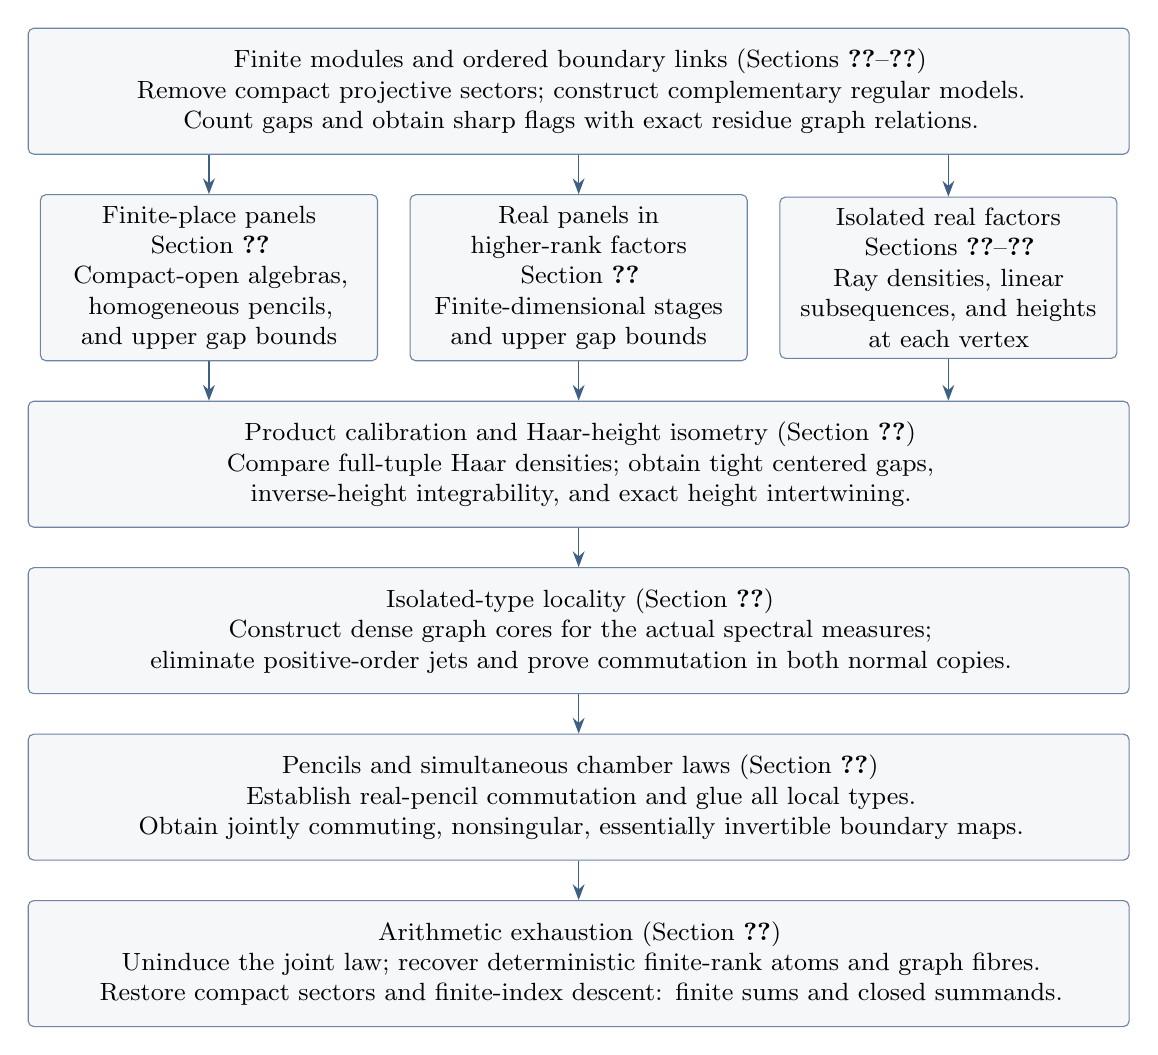
\begin{tikzpicture}[
  box/.style={draw=linkblue!65,rounded corners=2pt,fill=linkblue!4,
    align=center,text width=40mm,minimum height=16mm,inner sep=4pt,
    font=\small},
  wide/.style={box,text width=137mm},
  arrow/.style={-{Stealth[length=2mm]},draw=linkblue!85,line width=.6pt},
  node distance=5mm and 4mm]
\node[wide] (links) {Finite modules and ordered boundary links
  (Sections~\ref{sec:setup}--\ref{sec:transfer})\\
  Remove compact projective sectors; construct complementary regular models.\\
  Count gaps and obtain sharp flags with exact residue graph relations.};
\node[box,below=of links] (real) {Real panels in\\higher-rank factors\\
  Section~\ref{sec:panels}\\
  Finite-dimensional stages\\and upper gap bounds};
\node[box,left=of real] (finite) {Finite-place panels\\
  Section~\ref{sec:finite}\\
  Compact-open algebras,\\homogeneous pencils,\\and upper gap bounds};
\node[box,right=of real] (isolated) {Isolated real factors\\
  Sections~\ref{sec:ray}--\ref{sec:scale}\\
  Ray densities, linear\\subsequences, and heights\\at each vertex};
\node[wide,below=of real] (haar) {Product calibration and Haar-height isometry
  (Section~\ref{sec:heights})\\
  Compare full-tuple Haar densities; obtain tight centered gaps,\\
  inverse-height integrability, and exact height intertwining.};
\node[wide,below=of haar] (locality) {Isolated-type locality
  (Section~\ref{sec:locality})\\
  Construct dense graph cores for the actual spectral measures;\\
  eliminate positive-order jets and prove commutation in both normal copies.};
\node[wide,below=of locality] (gluing) {Pencils and simultaneous chamber laws
  (Section~\ref{sec:gluing})\\
  Establish real-pencil commutation and glue all local types.\\
  Obtain jointly commuting, nonsingular, essentially invertible boundary maps.};
\node[wide,below=of gluing] (arithmetic) {Arithmetic exhaustion
  (Section~\ref{sec:recovery})\\
  Uninduce the joint law; recover deterministic finite-rank atoms and graph fibres.\\
  Restore compact sectors and finite-index descent: finite sums and closed summands.};
\draw[arrow] (links.south) -- (real.north);
\draw[arrow] (links.south -| finite) -- (finite.north);
\draw[arrow] (links.south -| isolated) -- (isolated.north);
\draw[arrow] (real.south) -- (haar.north);
\draw[arrow] (finite.south) -- (haar.north -| finite);
\draw[arrow] (isolated.south) -- (haar.north -| isolated);
\draw[arrow] (haar) -- (locality);
\draw[arrow] (locality) -- (gluing);
\draw[arrow] (gluing) -- (arithmetic);
\end{tikzpicture}

 \caption{The geometric proof of arithmetic exhaustion. Each local branch
 enters product calibration with its own speed and domain statement;
 simultaneous commutation is established only afterwards.}
 \label{fig:proof-map}
\end{figure}

\subsection{Organization}
Section~\ref{sec:models} verifies the elementary arithmetic models.
Sections~\ref{sec:setup}--\ref{sec:transfer} construct the finite-module
framework and ordered sharp boundary links. The finite-place, isolated
real, and higher-component real arguments occupy
Sections~\ref{sec:finite}--\ref{sec:panels}; Table~\ref{tab:local-branches}
records their exact inputs to Section~\ref{sec:heights}.
Sections~\ref{sec:locality}--\ref{sec:gluing} prove locality and
simultaneous commutation. Section~\ref{sec:recovery} extracts the
arithmetic models and completes Theorem~\ref{thm:arithmetic-exhaustion}.
All geometric and analytic arguments needed for this theorem are given
in this article.

\FloatBarrier
\section{Elementary arithmetic correspondences}\label{sec:models}
The models in Theorem~\ref{thm:arithmetic-exhaustion} have an explicit
counting-space realization. We give the scalar transport and the
normality proof before beginning the geometric argument; neither depends
on arithmetic exhaustion. Projective induction is classical
\cite[Section~4]{Mackey1958}, and these coordinates also belong to the
finite-index bimodule calculus of \cite[Section~6.2]{Vaes2008}.

Throughout this section $\Gamma,\Lambda$ are arbitrary countably infinite
ICC groups, $M=L_\mu(\Gamma)$, and $N=L_\omega(\Lambda)$. Put
\[
 D=\Gamma\times\Lambda,\qquad
 \alpha((g,h),(g',h'))=\mu(g,g')\overline{\omega(h,h')}.
\]
For an isomorphism $\delta:A\to B$ of finite-index subgroups, its graph is
$C_\delta=\{(a,\delta(a)):a\in A\}\leq D$.

\subsection{Projective induction}
Let $C\leq D$ be a subgroup and let $\gamma$ be a normalized unitary
projective representation on a finite-dimensional space $V$, with
multiplier $\alpha|_{C\times C}$.  Write $X=D/C$ for left cosets.
Choose representatives $r_x\in D$, with $r_C=e$, and give each $x\in X$
a copy $V_x$ of $V$.  Set
$\mathcal H(C,\gamma)=\bigoplus_{x\in X}V_x$, with the counting
Hilbert norm.  For $s\in D$ put
\begin{equation}\label{eq:input-A1}
 \begin{split}
 c(s,x)&=r_{sx}^{-1}sr_x,\\
 U^X_s(x)&=
 \frac{\alpha(s,r_x)}{\alpha(r_{sx},c(s,x))}\,
 \gamma(c(s,x)):V_x\longrightarrow V_{sx}.
 \end{split}
\end{equation}

\begin{lemma}[Exact projective induction]
\label{lem:models-induction}
Equation~\eqref{eq:input-A1} defines a unitary projective representation
of $D$ with multiplier $\alpha$.  Changing the coset representatives
gives a unitarily equivalent bundle by unitary identifications of its
individual fibres.  If $C$ is the graph of a finite-index subgroup
isomorphism $A\to B$, the bundle has commuting normal $M$ and right
$N$ actions, and is bifinite.
\end{lemma}

\begin{proof}
The correction $c(s,x)$ belongs to $C$, and
\[
 c(s,tx)c(t,x)=c(st,x).
\]
Using the cocycle identity for $\alpha$ and the projective multiplication
of $\gamma$ in Equation~\eqref{eq:input-A1} gives
\begin{equation}\label{eq:calculus-transport-identity}
 U^X_s(tx)U^X_t(x)=\alpha(s,t)U^X_{st}(x).
\end{equation}
One can also check all the scalar factors at once in the central
extension with multiplication
$(z,s)(w,t)=(zw\alpha(s,t),st)$: the representation of its preimage
of $C$ is $(z,c)\mapsto z\gamma(c)$, and the equality
$sr_x=r_{sx}c(s,x)$ gives exactly the ratio in
Equation~\eqref{eq:input-A1}.  Thus this argument retains, rather than
discards, the fixed multiplier.

For explicit independence of representatives, suppose
$r'_x=r_xk_x$, where $k_x\in C$.  The identification from the new
coordinate copy of $V_x$ to the old one is
\[
 F_x=\alpha(r_x,k_x)^{-1}\gamma(k_x).
\]
Indeed identifying a fibre by $U_{r'_x}$ instead of $U_{r_x}$ has
precisely this effect.  Equation~\eqref{eq:calculus-transport-identity}
then gives $F_{sx}U'{}^X_s(x)=U^X_s(x)F_x$.

Now assume that $C$ is a graph.  Both coordinate groups act freely on
$X$.  For example, if $(g,e)r_xC=r_xC$, then
$r_x^{-1}(g,e)r_x\in C$ has second coordinate $e$, so $g=e$.
On an orbit of the first coordinate group choose a fibre $V_{x_0}$.
The unitary identification
\[
 \ell^2(\Gamma)\otimes V_{x_0}\longrightarrow
 \bigoplus_{g\in\Gamma}V_{(g,e)x_0},
 \qquad \delta_g\otimes\xi\longmapsto U^X_{(g,e)}\xi
\]
intertwines its action with $\lambda_\mu\otimes1$, since
$U_{(a,e)}U_{(g,e)}=\mu(a,g)U_{(ag,e)}$.  Hence it extends normally
to $L_\mu(\Gamma)$.  The same argument for the second coordinate
gives copies of $\lambda_{\bar\omega}$, which are the standard
normal representations of the generators acting by right adjoints
$\xi\mapsto\xi v_h^*$.  The two actions commute, because the product
cocycle has trivial mixed-coordinate factors.

The first coordinate orbits are indexed by $\Lambda/B$, and the
second coordinate orbits by $\Gamma/A$.  They are finite in number.
Each is a regular module with multiplicity $\dim_{\mathbb C}V$,
proving bifiniteness as well as the dimension formulas below.
\end{proof}

We next identify this construction with the Connes-product model in
Theorem~\ref{thm:arithmetic-exhaustion}.  This also supplies a direct normality
check of the subgroup action used to define that product.

\begin{lemma}[The graph-bundle unitary]
\label{lem:models-graph}
Let $\delta:A\to B$ be a finite-index subgroup isomorphism and let
$\sigma:A\to\mathcal U(V)$ have multiplier
$\beta=\mu|_{A\times A}/\delta^*\omega$.  Define
$\gamma(a,\delta(a))=\sigma(a)$.  Then
\[
 E(A,B,\delta,\sigma)=
 L^2(M)\mathbin{\bar\otimes}_{L_{\mu|A}(A)}
       (V\otimes L^2(N))
 \cong\mathcal H(C_\delta,\gamma).
\]
The unitary sends the vector $\xi$ in the fibre labelled by $x$ to
$U_{r_x}j\xi$, where
$j\xi=\widehat1\otimes(\xi\otimes\widehat1)$ in the displayed model.
\end{lemma}

\begin{proof}
On $V\otimes L^2(N)$ the subgroup action is
\[
 u_a(\xi\otimes\eta)=\sigma(a)\xi\otimes v_{\delta(a)}\eta.
\]
Its multiplier is $\beta(a,b)\omega(\delta(a),\delta(b))=\mu(a,b)$.
For normality, choose representatives $t$ for $B\backslash\Lambda$.
On the summand spanned by $\xi\otimes v_{\delta(a)}v_t$, the map
\begin{equation}\label{eq:calculus-absorption}
 \xi\otimes v_{\delta(a)}v_t
 \longmapsto\delta_a\otimes\sigma(a)^*\xi
 \quad\text{in }\ell^2(A)\otimes V
\end{equation}
is unitary and conjugates the subgroup action to
$\lambda_{\mu|A}\otimes1$.  To check the phase, applying $u_b$
before this map produces
\[
 \omega(\delta(b),\delta(a))
 \sigma(ba)^*\sigma(b)
 =\omega(\delta(b),\delta(a))\beta(b,a)\sigma(a)^*
 =\mu(b,a)\sigma(a)^*.
\]
Thus the left subgroup action is normal.  Its right $N$ action is
the standard action on the second factor and commutes with it.

Choose representatives $r$ for $\Gamma/A$.  As a right
$L_{\mu|A}(A)$ module, $L^2(M)$ has orthonormal free basis $u_r$;
the assertion follows directly from
$E_{L_{\mu|A}(A)}(u_r^*u_{r'})=\delta_{r,r'}1$.
The relative product therefore identifies with the orthogonal sum
\begin{equation}\label{eq:calculus-coset-model}
 E(A,B,\delta,\sigma)
 =\bigoplus_{r\in\Gamma/A}u_r\otimes(V\otimes L^2(N)).
\end{equation}
At its identity fibre the graph action is exactly
\[
 U_{(a,\delta(a))}j\xi
 =u_a\otimes(\xi\otimes v_{\delta(a)}^*)
 =j\sigma(a)\xi.
\]
For $g=ra$, balancing in Equation~\eqref{eq:calculus-coset-model}
gives the more explicit formula
\[
 U_{(g,h)}j\xi
 =\mu(r,a)^{-1}u_r\otimes
       \bigl(\sigma(a)\xi\otimes v_{\delta(a)}v_h^*\bigr).
\]
The last Fourier coordinate is $\delta(a)h^{-1}$, up to its displayed
unit scalar.  Thus two translated identity fibres are orthogonal
unless their labels in $D/C_\delta$ agree: equality of their first
cosets and last Fourier coordinates is exactly that coset equality.
Conversely these fibres exhaust every summand in
Equation~\eqref{eq:calculus-coset-model}.  They are an orthogonal,
transitive system with graph action $\gamma$ at the basepoint.
Finally
\[
 U_sU_{r_x}j
 =\frac{\alpha(s,r_x)}{\alpha(r_{sx},c(s,x))}
       U_{r_{sx}}j\gamma(c(s,x)),
\]
which proves that the stated unitary has exactly the transport
of Equation~\eqref{eq:input-A1}.
\end{proof}


\begin{corollary}[Elementary normality and dimensions]\label{cor:models-dimensions}
The correspondence $E(A,B,\delta,\sigma)$ is normal and bifinite. If
$n=\dim_{\mathbb C}V_\sigma$, then
\[
 \dim_M E(A,B,\delta,\sigma)=n[\Lambda:B],\qquad
 \dim E(A,B,\delta,\sigma)_N=n[\Gamma:A].
\]
\end{corollary}
\begin{proof}
Use Lemma~\ref{lem:models-graph} and the orbit decompositions in
Lemma~\ref{lem:models-induction}. Each free coordinate orbit gives $n$
regular copies, of module dimension $n$ with the unnormalized matrix
trace convention. The respective orbit counts are $[\Lambda:B]$ and
$[\Gamma:A]$.
\end{proof}

Finite direct sums and closed bimodule summands of these models remain
normal and bifinite: the two actions restrict normally to a reducing
subspace, and module dimension is additive and monotone under orthogonal
projections in the commutant
\cite[Theorem~10.2.1]{Jones2009}. The geometric problem is the converse:
starting from an arbitrary bifinite correspondence, recover enough
subgroup graphs to contain it. We now make the finite-index and compact
reductions needed for that construction.

\section{Finite-module realizations and local-field geometry}
\label{sec:setup}

The first analytic goal is to construct a finite regular realization
for each choice of an omitted left action on the tensor copies of the
correspondence. Each realization includes the other left actions and
the diagonal right action. These realizations supply the finite traces
used to construct boundary measurements in Section~\ref{sec:links}.
We first remove the compact part of one conjugation action, then form
the tensor copies and the induced transports for the omitted source
action. Conjugation by these transports gives a genuine action of its
ambient group on the finite algebra. The remaining subsections describe
the geometric data to be read from the source-lattice Fourier indices.

Fix a nonzero
bifinite $L_\mu(\Gamma)$--$L_\omega(\Lambda)$ correspondence $K$ as in
Theorem~\ref{thm:arithmetic-exhaustion}. A right action
of $L_\omega(\Lambda)$ is written as the projective representation
\[
 \rho(h)\xi=\xi v_h^*,\qquad
 \rho(h)\rho(k)=\overline{\omega(h,k)}\rho(hk).
\]
The left representation is denoted by $\pi(g)\xi=u_g\xi$.  Thus $\pi$
and $\rho$ commute, although their multipliers need not be trivial.
Conjugation by either representation is an ordinary group action.
All Hilbert spaces and von Neumann algebras considered below are
separable in the senses appropriate to their normal representations.


\subsection{Compact reduction and finite-index return}

We will prove the geometric reconstruction first for an actual ICC
lattice $\Gamma<G$ and under the condition
\begin{equation}
 \Ad\rho\ \text{on}\
 L^2\bigl(\pi(L_\mu(\Gamma))',\operatorname{tr}\bigr)
       \ominus\mathbb C1
 \quad\text{has no nonzero finite-dimensional subrepresentation}.
 \label{eq:setup-weak-mixing}
\end{equation}
Here the commutant is a finite factor, equipped with its normalized
trace.  The following reductions justify this choice.  Their final use,
after the geometric partition has been constructed, is made in
Section~\ref{sec:recovery}.

\begin{lemma}[Twisted regular absorption]
\label{lem:setup-twisted-absorption}
Let $\alpha,\nu$ be normalized scalar cocycles on a countable group
$L$, and let $v$ be a $\nu$-projective unitary representation on a
Hilbert space $V$.  Then
\[
 \lambda_\alpha\otimes v
       \simeq \lambda_{\alpha\nu}\otimes1_V.
\]
If $L$ is ICC and $V$ is finite-dimensional, tensoring a finite normal
$L_\alpha(L)$-module with $v$ gives a finite normal
$L_{\alpha\nu}(L)$-module.  Any additional operators commuting with
every $v_h$ are preserved by the absorption identification.
\end{lemma}

\begin{proof}
On $\ell^2(L)\otimes V$ use the unitary
\[
 T(\delta_g\otimes\xi)=\delta_g\otimes v_g^*\xi.
\]
Indeed,
\begin{align*}
 T(\lambda_\alpha(h)\otimes v_h)T^*
          (\delta_g\otimes\xi)
 &=\alpha(h,g)\delta_{hg}\otimes v_{hg}^*v_hv_g\xi\\
 &=\alpha(h,g)\nu(h,g)\delta_{hg}\otimes\xi.
\end{align*}
A finite normal module over a finite factor embeds in finitely many
copies of the regular module
\cite[Theorems~10.1.1 and~10.2.1]{Jones2009}.  When $L$ is ICC both twisted group
algebras are factors.  Applying this unitary to such an embedding proves the second
assertion.  The formula also proves the last assertion directly.
\end{proof}

\begin{lemma}[Compact commutant reduction]
\label{lem:setup-compact-reduction}
Let $K$ be a nonzero bifinite
$L_\mu(\Gamma)$--$L_\omega(\Lambda)$ correspondence, with both groups
ICC.  There is a finite-index subgroup $\Lambda_0\leq\Lambda$ such
that the restriction of $K$ to the right subgroup factor is a finite
orthogonal sum of blocks
\[
 K_c=V_c\otimes K'_c,
 \qquad
 \pi(g)|_{K_c}=1\otimes\pi'_c(g),
 \qquad
 \rho(h)|_{K_c}=v^c_h\otimes\rho'_c(h)
       \quad(h\in\Lambda_0).
\]
The spaces $V_c$ are finite-dimensional.  The $v^c_h$ are normalized
projective matrix representations, with multipliers $\nu_c$, and
\begin{equation}
 \rho'_c(h)\rho'_c(k)
  =\frac{\overline{\omega(h,k)}}{\nu_c(h,k)}\rho'_c(hk).
 \label{eq:setup-reduced-right-multiplier}
\end{equation}
Each $K'_c$ is a finite normal module on both sides and satisfies
Equation~\eqref{eq:setup-weak-mixing} for its reduced representations.
There is no assertion that any $v^c$ has finite image.
\end{lemma}

\begin{proof}
Put $M=L_\mu(\Gamma)$, $N=L_\omega(\Lambda)$, and
$P=\pi(M)'$.  Finite $M$-module dimension makes $P$ a finite factor.
Moreover $N^{\mathrm{op}}\subset P$ has finite index.  To see the
latter without assuming the endpoint actions are mutual commutants,
regard $K$ as the equivalence module for the mutually commuting factors
$\pi(M)$ and $P$.  It has finite nonzero $P$-dimension.  Finitely many
copies of it therefore contain $L^2(P)$ as a $P$-module.  Their
restrictions to $N^{\mathrm{op}}$ are finite, by the original right
finiteness of $K$.  Consequently $L^2(P)$ has finite
$N^{\mathrm{op}}$-dimension, which is the index assertion.  We use
the standard finite-module and index facts in this argument in the
normal, trace-preserving convention; see
\cite{Jones1983} and \cite[Proposition~2.1]{PimsnerPopa1986}.

Let $D_c$ be the bounded elements of $P$ whose $\Ad\rho$-orbits are
precompact in $L^2(P)$.  The compact vectors of a unitary representation
form its closed almost-periodic subspace: they are the closed span of
its finite-dimensional subrepresentations.  Bounded compact elements
are closed under adjoints and products, since
\[
 \|xy-x'y'\|_2
 \leq \|x\|_\infty\|y-y'\|_2
       +\|x-x'\|_2\|y'\|_\infty
\]
on uniformly bounded sets.  Their bounded balls are strongly closed,
because bounded strong convergence in a finite von Neumann algebra
implies $L^2$ convergence.  They therefore form a von Neumann
subalgebra.  They are dense in the compact Hilbert subspace: the
nearest-point projection in $L^2(P)$ onto each closed operator-norm
ball is equivariant and nonexpansive, so maps compact orbits to compact
orbits, and these projections approximate every $L^2$ vector.

Twisted conjugation on $L^2(N)\ominus\mathbb C1$ has no nonzero
finite-dimensional subrepresentation.  Indeed, the diagonal of a
finite-rank invariant orthogonal projection in the Fourier basis is
constant on conjugacy classes: scalar conjugation phases disappear
from the diagonal.  The diagonal is summable.  Every nonidentity
conjugacy class is infinite, so all its entries vanish.  Only the
identity vector remains.  The trace-preserving expectation
$E_{N^{\mathrm{op}}}:P\to N^{\mathrm{op}}$ is equivariant and
$L^2$-contractive.  It follows that
\[
 E_{N^{\mathrm{op}}}(x)=\operatorname{tr}(x)1
             \quad(x\in D_c).
\]
By the finite-index expectation inequality there is $\varepsilon>0$
such that $E_{N^{\mathrm{op}}}(x)\geq\varepsilon x$ for $x\geq0$.
Thus a nonzero projection $q\in D_c$ has
$\operatorname{tr}(q)\geq\varepsilon$.  A finite algebra with such a
lower bound has only finitely many orthogonal nonzero projections,
and is finite-dimensional.

Restrict $\Lambda$ to the finite-index subgroup $\Lambda_0$ fixing
all the central blocks of $D_c$.  A central block $z$ now reduces both
endpoint actions.  Write
\[
 zK=V_c\otimes K'_c,
 \qquad zD_c=\mathcal B(V_c)\otimes1.
\]
The left action commutes with $D_c$, hence is $1\otimes\pi'_c$.
Choose normalized matrix implementers $v^c_h$ for
$\Ad\rho(h)|_{zD_c}$.  Uniqueness of an implementer up to scalar
gives
$v^c_hv^c_k=\nu_c(h,k)v^c_{hk}$, with $\nu_c$ a normalized cocycle.
After removing these implementers, $\rho(h)$ belongs to the
commutant of $\mathcal B(V_c)$ and therefore has the asserted tensor
form.  Multiplication gives
Equation~\eqref{eq:setup-reduced-right-multiplier}.

Normality and finiteness of $\pi'_c$ follow by taking a matrix corner
of the finite normal left module.  For the right action, first embed
the original restricted $\rho$ in a finite multiple of the
$\overline\omega|_{\Lambda_0}$-regular representation.  This is
possible because finite-index restriction preserves finite module
dimension.  Tensor with $\overline{v^c}$.  Lemma~
\ref{lem:setup-twisted-absorption} gives a finite normal module with
multiplier $\overline{\nu_c}\,\overline\omega$.  In
$\overline V_c\otimes V_c$ the vector corresponding to the identity
matrix is fixed by $\overline{v^c_h}\otimes v^c_h$.  Tensoring that
line with $K'_c$ exhibits $\rho'_c$ as a summand of the preceding
normal finite representation.  This proves its normality for exactly
the multiplier in Equation~\eqref{eq:setup-reduced-right-multiplier}.
Equivalently, its right factor has cocycle
$\omega|_{\Lambda_0}\nu_c$.

Finally, a compact vector in the reduced commutant embeds as
$1_{V_c}\otimes\xi$ on $zK$ and as zero on the other blocks.  It is
compact for $\Lambda_0$, and hence for $\Lambda$: the latter orbit
is contained in a finite union of translates of the former compact
orbit closure.  It therefore belongs to $L^2(D_c)$.  Its intersection
with the reduced commutant on this block is scalar.  This proves
Equation~\eqref{eq:setup-weak-mixing}.
\end{proof}

\begin{lemma}[Finite-index restriction and return]
\label{lem:setup-finite-index-induction}
Let $\Gamma_0\leq\Gamma$ and $\Lambda_0\leq\Lambda$ have finite
index, and restrict both cocycles literally to these subgroups.  Every
$M$--$N$ correspondence is a summand of the two-sided induction of
its restriction.  The inclusions are given, on the respective sides,
by
\begin{align}
 J_L\xi&=[\Gamma:\Gamma_0]^{-1/2}
       \sum_{r\Gamma_0\in\Gamma/\Gamma_0}
              u_r\otimes\pi(u_r)^*\xi,
       \label{eq:setup-left-induction}\\
 J_R\xi&=[\Lambda:\Lambda_0]^{-1/2}
       \sum_{\Lambda_0s\in\Lambda_0\backslash\Lambda}
              (\xi v_s^*)\otimes v_s.
       \label{eq:setup-right-induction}
\end{align}
These are bimodular isometries, with all scalar cocycles included.
Restriction and induction preserve bifiniteness.  An ICC group stays
ICC on finite-index restriction.
\end{lemma}

\begin{proof}
The $u_r$ in Equation~\eqref{eq:setup-left-induction} are an
orthonormal right basis for $L^2(M)$ over the subgroup factor, because
\[
 E_{L_{\mu|\Gamma_0}(\Gamma_0)}(u_r^*u_{r'})
   =\delta_{r,r'}1.
\]
The analogous left-basis identity for the $v_s$ is
$E_{L_{\omega|\Lambda_0}(\Lambda_0)}(v_sv_{s'}^*)
=\delta_{s,s'}1$.  The relative tensor-product inner products give
the asserted isometries.

For explicit left equivariance, if $gr=r'a$ with $a\in\Gamma_0$,
then
\[
 u_gu_r=\frac{\mu(g,r)}{\mu(r',a)}u_{r'}u_a.
\]
Move $u_a$ across the balanced tensor product.  The identity
$u_{r'}^*u_g=(\mu(g,r)/\mu(r',a))u_au_r^*$ shows that the term is
exactly the $r'$-term of $J_L(\pi(u_g)\xi)$.  The right calculation
is the same calculation in the opposite algebra.  Explicitly, when
$sh=at$ with $a\in\Lambda_0$, one has
\[
 v_sv_h=\frac{\omega(s,h)}{\omega(a,t)}v_av_t,
 \qquad
 v_hv_t^*=\frac{\omega(s,h)}{\omega(a,t)}v_s^*v_a.
\]
Balancing $v_a$ proves right equivariance of
Equation~\eqref{eq:setup-right-induction}.  The other endpoint action
commutes with every operation.  Thus the two maps compose to a
bimodular isometry into two-sided induction, whose range is a closed
summand.  The finite basis formulas also show preservation of finite
module dimensions.

If an element of $\Gamma_0$ has finite conjugacy class in
$\Gamma_0$, its conjugacy class in $\Gamma$ is a finite union of
translates of that class.  ICC of $\Gamma$ forces the element to be
the identity.  This proves the last assertion.
\end{proof}

For a source in $\mathscr K$, choose the actual isomorphism of
finite-index subgroups in Definition~\ref{def:class}.  Its image is
a finite-index subgroup of a reference lattice, hence itself a lattice
in the same ambient group.  Pull the scalar cocycle through that
isomorphism, without modifying it by a finite kernel.  The restrictions
retain property~(T) and ICC, as well as bifiniteness; property~(T)
permanence is used in its usual finite-covolume and finite-index forms
\cite[Theorem~1.7.1]{BHV2008}; see also the original finite-covolume
statement in \cite[Theorem~3]{DelarocheKirillov1968}.  Lemmas~\ref{lem:setup-compact-reduction} and
\ref{lem:setup-finite-index-induction} now reduce the geometric work
to the actual-lattice, weakly mixing setting.  Restoring $V_c$ after a
partition of $K'_c$ tensors every atom with $V_c$ and restores the
original exact right multiplier.  It changes neither the atom
permutations nor their freeness.  This observation will be used only
after that partition is proved.


\subsection{Tensor copies and complementary regular realizations}

From now until Section~\ref{sec:recovery}, let $\Gamma<G$ be an
actual ICC lattice and impose Equation~\eqref{eq:setup-weak-mixing}.
For a comparison of two source copies we use two copies of $K$; for
two comparisons sharing their first copy we use three. The right
comparison group acts diagonally. We omit one left source action from
the regular model so that its induced transports remain available on
$G/\Gamma$.


Take $m=1$ or $2$, and put
\[
 H=K^{\otimes(m+1)},\qquad
 R=\Gamma_1\times\cdots\times\Gamma_m\times\Lambda.
\]
The slots of $H$ are numbered $0,\ldots,m$; $\pi_j$ denotes the
left representation in slot $j$.  Let $W$ be the representation of
$R$ given by the $\pi_j$, $j\geq1$, and diagonal $\rho$.  Its split
multiplier is
\begin{equation}
 \alpha_R\bigl((g_1,\ldots,g_m,h),(g'_1,\ldots,g'_m,h')\bigr)
   =\prod_{j=1}^m\mu(g_j,g'_j)
        \overline{\omega(h,h')}^{\,m+1}.
 \label{eq:setup-tensor-multiplier}
\end{equation}

\begin{lemma}[Complementary regularity]
\label{lem:setup-normal-tensors}
The representation $W$ is normal and finite over the twisted factor
for $R$.  The same assertion holds with any one of the slots omitted
instead of slot zero.  The joint commutant of all $\pi_j(\Gamma)$,
$0\leq j\leq m$, and diagonal $\rho(\Lambda)$ is scalar.
\end{lemma}

\begin{proof}
Embed the omitted slot in a finite regular multiple for its
$\overline\omega$-projective right representation.  At that regular
index absorb the diagonal right actions of the remaining slots by
Lemma~\ref{lem:setup-twisted-absorption}.  This use of absorption
allows an infinite-dimensional auxiliary tensor space.  The
absorbing unitaries are formed from the other slots' $\rho(h)$ and
therefore commute with all their $\pi_j(g)$.  After absorption,
the $\Lambda$ action is regular with multiplier
$\overline\omega^{\,m+1}$, and each remaining $\pi_j$ can
independently be embedded in a finite regular multiple for
$L_\mu(\Gamma_j)$.  The resulting whole representation is a
subrepresentation of a finite regular multiple for exactly
Equation~\eqref{eq:setup-tensor-multiplier}.  The construction is
symmetric in the omitted slot.

Write $P=\pi(M)'$.  The final joint commutant is
$(P^{\overline\otimes(m+1)})^{\Ad\rho^{\otimes(m+1)}}$.
Condition~\eqref{eq:setup-weak-mixing} makes this fixed algebra
scalar.  For completeness, an invariant tensor with a factor in
$L^2(P)\ominus\mathbb C1$ gives a Hilbert--Schmidt intertwiner
between that factor's representation and another unitary
representation.  The positive compact operator obtained by composing
with its adjoint has a nonzero finite-dimensional invariant spectral
space, contrary to weak mixing.  Decompose each tensor factor as
$\mathbb C1\oplus(L^2(P)\ominus\mathbb C1)$ to apply this
argument to every nonconstant summand.
\end{proof}

Choose a column realization
\[
 H=eL^2(B)^k,\qquad e\in M_k(B),\qquad
 d=(\Tr_k\otimes\tau_B)(e)>0.
\]
Here $B$ is the opposite of the $\alpha_R$-twisted factor of $R$.
Using the adjoints of the opposite canonical generators identifies
it with the $\overline{\alpha_R}$-twisted group factor: write these
generators as $w_r$.  Thus $W_r$ is right multiplication by $w_r^*$,
which indeed has multiplier $\alpha_R$.

Set
\begin{equation}
 Y=G/\Gamma,\qquad
 \mathcal H=L^2(Y;H),\qquad
 \mathcal N=L^\infty(Y)\overline\otimes eM_k(B)e.
 \label{eq:setup-induced-model}
\end{equation}
Give $Y$ its invariant probability measure.  The trace on
$\mathcal N$ is
\[
 \operatorname{tr}_{\mathcal N}(A)
    =d^{-1}\int_Y(\Tr_k\otimes\tau_B)(A(y))\,dy,
\]
whereas the Hilbert norm of a column uses the unnormalized entrywise
trace sum.  All finite-matrix estimates permit rectangular products.
Whenever a family of coefficient algebras is varied, coefficient
traces are normalized and matrix sizes are fixed, or the corresponding
Hilbert-norm factors are retained explicitly.  An operator-norm bound
alone is not a bound independent of arbitrary trace rescaling.

Choose a Borel section $d_0:Y\to G$ and write
\[
 c(a,y)=d_0(ay)^{-1}ad_0(y),\qquad
 X_a(y)=\pi_0(c(a,y)),\qquad
 (U_af)(ay)=X_a(y)f(y).
\]
These transports compose up to a scalar function of modulus one on
the base.  More explicitly,
\[
 X_a(by)X_b(y)
   =\mu\bigl(c(a,by),c(b,y)\bigr)X_{ab}(y).
\]
Conjugation on base-decomposable operators is therefore a genuine
action, denoted by $\sigma=\Ad U$.

\begin{proposition}[Induced finite algebras]
\label{prop:setup-induced-algebras}
The transports $U_a$ are strongly continuous in $a$, and $\sigma$
preserves the trace on $\mathcal N$.  For $1\leq j\leq m$, let
$R'_j$ be $R$ with $\Gamma_j$ omitted, put
$\beta_j=\Ad W_{\Gamma_j}$, and let $\mathcal A_j$ be the
commutant of the base multipliers and $W|_{R'_j}$.  Then
\[
 (\mathcal A_j)^{\beta_j}=\mathcal N,
 \qquad
 (\mathcal A_j)^\sigma
 \ \text{has a faithful finite $\beta_j$-invariant trace},
 \qquad
 \mathcal N^G=\mathbb C1.
\]
\end{proposition}

\begin{proof}
Translation is continuous in measure on measurable maps on the
finite-measure quotient.  Applied to the Borel section, this shows
that $c(a,y)$ varies continuously in measure as a discrete-valued
map.  One can verify the assertion first on compact sets where the
section is continuous, by Lusin approximation, and then remove sets
of arbitrarily small measure.  The corresponding projective
unitaries are bounded, so their multiplication operators, together
with the base translations, vary strongly on $\mathcal H$.
Conjugation of the corner is inner at each fibre and translation
preserves base probability.  Thus $\sigma$ preserves the displayed
trace.  The first fixed-algebra identity is simply the commutant of
all of $W$ in the decomposable algebra.

For the second identity, undo induction.  If $A(y)$ is a
$\sigma$-invariant decomposable field, lift it, for
$g=d_0(y)\gamma$, as
\[
 \widetilde A(g)=\pi_0(\gamma)^*A(y)\pi_0(\gamma).
\]
The cocycle covariance makes this field left $G$-invariant.  It is
therefore almost everywhere constant, with value $T$, and right
$\Gamma$-covariance says that $T$ commutes with $\pi_0(\Gamma)$.
It also commutes with $W|_{R'_j}$.  Conversely every such $T$ gives
a fixed field.  Consequently $(\mathcal A_j)^\sigma$ is the
commutant of the complementary regular representation obtained by
omitting slot $j$.  Lemma~\ref{lem:setup-normal-tensors} makes this
commutant finite; its normalized trace is $\beta_j$-invariant,
since the remaining slot acts by unitaries in that commutant.
Including all the slots and using the last assertion of that Lemma
gives $\mathcal N^G=\mathbb C1$.
\end{proof}


\subsection{The source groups and full versus partial mixing}

The induced algebra has only scalar whole-group invariants. To turn
that fact into limits along Cartan paths, we need the mixing theorem
for the actual root-generated groups. We record the group conventions
here; the length and matrix coordinates are introduced afterwards.
We use the standard parabolic and root-group structure,
Cartan--Iwasawa decompositions, central-cover facts, root-generated
simplicity, and highest-weight theory
\cite{Borel1991,BT1965,BruhatTits1972,BruhatTits1984,Tits1964,Humphreys1972}.

\begin{convention}[Factors and panel groups]
\label{conv:setup-panels}
At a complex place the local group is regarded as a real Lie group.
The noncompact property-(T) archimedean factors are the higher-rank
ones and the groups locally isomorphic to $Sp(n,1)$, $n\geq2$, or
$F_{4(-20)}$.  At a finite place the factors have relative rank at
least two. For higher-rank property~(T), see
\cite[Theorem~6]{DelarocheKirillov1968}; the real rank-one
classification and its Kostant attribution are recalled in
\cite[Section~3.3 and Theorem~3.5.4]{BHV2008}. Relative rank one
at a finite place gives an unbounded action on the Bruhat--Tits tree
and is incompatible with property~(T) \cite[Remark~1.6.3]{BHV2008}.

In a rank-one semisimple Levi position exactly one almost simple
factor is isotropic.  Its minimal boundary is the full panel residue.
The compact and toric normal factors of the Levi act trivially on
this boundary.  Source transports use its root-generated group.
When an algebraic central cover is needed, use the subgroup generated
by its lifted unipotent radicals.  The root-group isomorphisms below
map this subgroup onto the effective root-generated group with finite
central kernel.  Every application of Howe--Moore takes invariants
for this root-generated group or lift.
Projectivities use the effective adjoint group; the adjoint point
group is allowed for changes of frame.  We never replace a full flag
by an oriented or topological covering flag.
\end{convention}

To check these conventions, take two opposite parabolics.  Their
refinement spaces identify with the flags of the common Levi.  On
the transverse open cell, the radical is removed by projection, and
Levi transport acts by its inner algebraic automorphisms.  The
anisotropic normal factors are compact and have no flag coordinate
in the relative building; the central torus acts trivially there as
well.  Simply connected covers have finite central kernel, contain
the root-generated groups in their images on points, and have image
of at most finite index in the adjoint point group.  They have the
same Bruhat flag orbits.  At real places any remaining ineffective
or component extension is compact or finite.

For the cover assertion, a central covering induces an isomorphism
on the corresponding relative root groups, so its image contains
the subgroup generated by the unipotent radicals
\cite[Theorem~2.20(iii) and Proposition~2.24(ii)]{BT1972Complements}.
Its kernel on local points is finite.  For a central kernel $C$,
the rational-point quotient injects into $H^1(k,C)$, which is finite
over the present local fields
\cite[Propositions~1.12 and~1.17, Theorem~6.1]{BorelSerre1964}.
This proves the finite-index assertion directly; no stronger
identification of all rational points with the root-generated
group is needed.


\begin{lemma}[Product mixing and partial escape]
\label{lem:setup-product-mixing}
For the action on $L^2(\mathcal N)$, escape in every simple factor
gives weak operator convergence to the projection onto constants.
If a path is the identity outside a subproduct $G_0$ and escapes in
every factor of $G_0$, its weak limit is the projection onto
$L^2(\mathcal N)^{G_0}$, equivalently the conditional expectation
onto $\mathcal N^{G_0}$.  On the orthogonal complement of a simple
factor's invariants, its matrix-coefficient decay remains uniform
after composition with arbitrary commuting group unitaries.
\end{lemma}

\begin{proof}
Use the Howe--Moore theorem for the noncompact isotropic almost
simple root-generated groups and their root-generated lifts from
Convention~\ref{conv:setup-panels} \cite{HoweMoore1979}; an independent proof with this root-generated group convention is given in \cite[Theorem~1.1 and Definition~4.23]{Ciobotaru2015}.
We first justify the type-I
input for these actual groups.  For an isotropic simple factor
$\mathbf H$ over $k$, choose a nonzero parabolic unipotent radical
$\mathbf U$.  The $k$-span of the $\mathbf H(k)$-conjugates of
$\operatorname{Lie}(\mathbf U)$ is a nonzero invariant Lie ideal,
hence all of $\operatorname{Lie}(\mathbf H)$.  Choose a basis
$X_1,\ldots,X_d$ from these conjugate subspaces.  The map
\[
 (t_1,\ldots,t_d)\longmapsto\prod_{j=1}^d\exp(t_jX_j)
\]
has invertible differential at zero and takes values in
$\mathbf H(k)^+$.  The local-field inverse function theorem makes
this subgroup open; at finite places see
\cite[Proposition~1.11]{Gloeckner2008}.  The same proof applies to
the root-generated subgroup of an algebraic simply connected cover.
At an archimedean place, the generating unipotent groups are connected,
so the root-generated group is connected.  Being open as well, it is
the identity component of the ambient real algebraic group; for a
complex group, use restriction of scalars to $\mathbb R$.  The same
applies to its algebraic lift.  These groups are therefore type~I by
\cite[Theorem~1]{Dixmier1957}.  At a finite place, the ambient reductive
group of local points is type~I \cite{Bernstein1974}, and type~I passes
to its open root-generated subgroup
\cite[Proposition~6.E.21(1)]{BekkaHarpe2019}.

Restrict a separable unitary representation $\pi$ to one simple
factor $S$.  Its type-I decomposition with multiplicity is
\[
 \mathcal H=\int_{\widehat S}^{\oplus}
       (H_\xi\otimes M_\xi)\,d\eta(\xi),\qquad
 \pi(s)=\int_{\widehat S}^{\oplus}(\xi(s)\otimes1)\,d\eta(\xi).
\]
In this central decomposition, every unitary commuting with $S$
acts fibrewise as $1\otimes V_\xi$
\cite[Propositions~5.4.7 and~8.6.4, Theorem~8.6.6]{Dixmier1977};
see also \cite[Theorem~7.32]{Folland2015}.  This is the decomposition
of the restriction to $S$, so no invariance of a finer decomposition
of the other factors is required.  For finite tensor sums in a
nontrivial fibre, uniformly over the unitaries $V_\xi$,
\[
 \left|\left\langle(\xi(s)\otimes V_\xi)
       \sum_j e_j\otimes u_j,\sum_k f_k\otimes v_k\right\rangle\right|
 \leq\sum_{j,k}|\langle\xi(s)e_j,f_k\rangle|
                    \|u_j\|\,\|v_k\|.
\]
Howe--Moore makes the right side tend to zero along escape.
Approximation by finite tensor sums is uniform because all operators
have norm one.  For arbitrary fixed fibre vectors the bound
$\|a_\xi\|\,\|b_\xi\|$ is integrable.  Dominated convergence
therefore proves the stated uniform decay off the $S$-invariants.

Let $P_i$ project onto the invariants of the $i$th simple factor.
These projections commute with every group action and with each
other.  Expand the identity as the finite sum of the mutually
orthogonal products obtained from $\prod_i(P_i+(1-P_i))$.
In every sector containing $1-P_i$, the uniform decay just proved
kills its coefficients when that factor escapes, even while all
other factor translations vary.  Thus for all-factor escape the
weak limit is $\prod_iP_i$, which is the projection onto constants
by Proposition~\ref{prop:setup-induced-algebras}.  For partial escape,
expand only over the factors of $G_0$; the other translations are the
identity.  The limit is the projection onto
$L^2(\mathcal N)^{G_0}$, namely the trace-preserving conditional
expectation.  The same argument applies to the simple Levi factors
used later.
\end{proof}


\subsection{Panel groups, Cartan coordinates, and Haar volumes}

The following geometric facts will specify the Fourier-index data used
by the boundary measurements. At a panel, only one noncompact rank-one
Levi factor acts on the residue; on a Cartan path, exact root coordinates
will determine which flag coordinates survive.

An archimedean panel inside a higher-rank component cannot have
noncompact Lie algebra $\mathfrak f_{4(-20)}$: its complexification
would have to occur as a component of a proper absolute Dynkin
subdiagram, and the Dynkin list has no such occurrence.  At a finite
place the effective rank-one Lie algebra is simple also over
$\mathbb Q_p$.  Indeed after restriction of scalars its absolutely
simple factors form one Galois orbit, so a $\mathbb Q_p$-ideal is
either zero or the whole algebra.  An adjoint automorphism centralizing
an open subgroup centralizes all sufficiently small inner
exponentials, and hence this Lie algebra; it is therefore the
identity.  These assertions concern the ambient local groups, not a
discreteness assumption on a lattice projection.

Let $\Pi$ be the union of the simple \emph{indivisible} relative
roots of the factors.  A face of type $I\subset\Pi$ has strictly
positive simple coordinates exactly in $I$; opposition of types
is denoted by a star.  Choose a special maximal compact in each
factor.  Cartan and Iwasawa decompositions can first be made on the
simply connected covers and then descended.  Write $\mu(g)$ for the
Cartan vector only when its argument is a local-group element; this
use of $\mu$ is distinct from the scalar two-cocycle
$\mu(g,h)$.  For a positive root $\alpha$, put
\[
 m_\alpha=\dim_{k}\mathfrak g_\alpha
     \quad\hbox{at a finite place},
 \qquad
 2\rho=\sum_{\alpha>0}m_\alpha\alpha,
\]
and use the analogous real restricted-root multiplicities at
archimedean places.  Double roots are included in this sum.  The
fundamental coweight rays $e_i$ are dual to the simple indivisible
roots.

\begin{convention}[Exact finite-place translation coordinates]
\label{conv:setup-exact-lengths}
At a finite place use the module absolute value, with
$|\varpi|=q^{-1}$.  The Cartan vector is the actual dominant
translation vector of a Cartan representative in the split
centralizer: its pairing with every centralizer character is the
exact logarithm of that character's module.  We do not replace this
by a coarsely equivalent length in identities involving heights.
All displacements and offsets along $e_i$ range on a sufficiently
divisible mesh in this logarithmic translation lattice.  Cocharacter
rationality and common multiples of relative coroot translations
and central isogenies ensure that these elements and their
semisimple projections to every standard Levi have lifts in the
corresponding root-generated covering groups.  There are only finitely
many standard Levis, so one divisible mesh suffices.  At real places
the corresponding split exponentials lie in the generated identity
lift.  No argument at a finite place requires every real
parameter to be an actual split displacement.
\end{convention}

Bounded parts of the centralizer act equicontinuously, with bounded
inverse, on the relevant weight spaces.  This permits compact frames
while keeping the character normalization exact.

\begin{lemma}[Haar size of Cartan shells]
\label{lem:setup-haar-shells}
For a bounded-thickness shell about a dominant vector $L$, its Haar
measure is at most $C\exp(2\rho(L))$.  For one fixed sufficiently
large thickness, there is also a lower bound
$c\exp(2\rho(L))$.  The constants are independent of $L$ on the
permissible Cartan mesh.  The analogous assertions hold for the
finite product, with the sum of the factors' $2\rho$.
\end{lemma}

\begin{proof}
At a real place use the Cartan density, a product of the appropriate
powers of $\sinh\alpha(L)$.  The upper bound follows on every fixed
bounded neighborhood.  For the lower bound, even when $L$ lies on a
wall, choose inside the shell one fixed bounded offset box whose
simple coordinates are bounded away from zero.  On this box every
positive-root factor is bounded below by a fixed multiple of its
exponential.  The box has fixed positive Euclidean volume.

At a finite place the Cartan double coset has measure
$[K:K\cap aKa^{-1}]$ times the fixed compact measure.  This index is
comparable to $\exp(2\rho(L))$.  One can see the uniform comparison
in compact root charts: a sufficiently small analytic compact open
subgroup has product coordinates in negative-root, centralizer, and
positive-root directions.  Under conjugation by the dominant
translation, its intersection is obtained by shrinking the expanding
root lattices.  The index is the product of their module indices,
with exponent $\sum_{\alpha>0}m_\alpha\alpha(L)$.  Equivariant
exponentials on small root lattices and parabolic product uniqueness
give this calculation; changing the compact frame changes the small
subgroups by a uniformly bounded index.  Other Cartan representatives
are within bounded distance of the chosen split mesh.  This proves
both bounds there.  Multiplication of Haar measures gives the product
assertion.
\end{proof}

Fixed left or right multiplication changes vector distances by a
bounded amount.  We use ordinary compact-rotation probabilities on
flags, or equivalently the Haar measure classes in their root
coordinates.  Proper algebraic incidence degeneracies have measure
zero.  All incidence and Weyl positions are those of the relative
spherical building.  A prescribed reduced longest gallery from a
chamber parametrizes its open opposition cell by successive panel
coordinates, with both measure-null directions preserved; this is
the ordered unipotent factorization of the Bruhat cell.  The same
statement holds at finite places.


\subsection{Compactified matrices and admissible scalar tests}

The measured geometric index will always lie in a copy $\Gamma_j$ of
the source lattice, inside its known ambient local group. We now give
a compact matrix description of the flags and residual projectivities
that can survive as that index escapes. This description is algebraic
at finite places; only its scalar observables will act on our complex
Hilbert spaces.


For each relative vertex type choose a highest-line representation
as follows.  Take the determinant line of the relevant parabolic
nilradical in an exterior power and the cyclic submodule it generates.
Over a splitting field, choose a compatible positive system.  This
line is a highest line, with a weight strictly positive on the omitted
absolute nodes and zero on the complementary coroots.  Its relative
weight is a positive multiple of the relevant fundamental weight.
The cyclic highest-weight module is absolutely irreducible and its
top split space is one-dimensional.  Lowering along an omitted
absolute simple root produces a weight separated by a positive
multiple of just the corresponding relative simple root.  Every
other weight drops by a nonnegative combination involving that root.
Consequently a normalized Cartan matrix has rank-one limit exactly
when that simple gap diverges.

At a finite place these are $k$-rational modules, used only to form
compact projective matrix data.  Use compact-invariant lattice norms
and compact sup-norm frames, recording both the matrix and its inverse
up to projective normalization.  At an archimedean target, for Hilbert
highest-line amplifications use a real proximal module irreducible
on complexification, with a compact-invariant inner product.  Taking
higher tensor weights is allowed.  No Hilbert space is tensored with
a vector space over a nonarchimedean field.

\begin{lemma}[Face blocks and residual projectivities]
\label{lem:setup-face-blocks}
Let a sequence have diverging simple gaps of types $D$, and keep its
complementary gaps in a bounded window.  Its compactified matrix data
determine an image $D$-flag, a reverse $D^*$-flag, and an invertible
residual Levi transport between their transverse refinement spaces.
These data are independent of compact frame choices.  On a deeper
stratum the already determined image vertices persist.  On compact
transverse windows the residual rank-one panel lengths differ by
bounded amounts from the actual omitted Cartan gaps.
\end{lemma}

\begin{proof}
Pass to convergent compact Cartan frames.  In each highest-weight
module, precisely the weights with maximal value on the open face
survive projective normalization.  They are the submodule generated
from the highest line by the complementary Levi.  Bounded
complementary gaps keep the surviving block and its inverse bounded
in those frames.  Thus the surviving block acts by an invertible Levi
transformation.  The same analysis of the inverse matrix identifies
the reverse face.

Equivalently, write an ordinary flag in the open Bruhat cell
transverse to the reverse face.  Conjugating its radical coordinates
by the Cartan translation contracts the coordinates belonging to the
diverging gaps; the complementary Levi coordinates remain.  First
project to the reverse refinement space, then apply the surviving
Levi transformation.  This is the intrinsic residual projectivity.
A change of compact frame conjugates these coordinates by the
corresponding compact Levi projectivity and leaves the intrinsic map
unchanged.  Passing to a deeper stratum preserves all preceding image
vertices.  In a face omitting one type in a higher-rank component,
the surviving rank-one split displacement is exactly that omitted
coordinate; bounded frames change its length by a uniformly bounded
amount.  The argument works simultaneously for one omitted type in
several components.

In an archimedean module the surviving top block contains the highest
lines of all incident flags, and those lines span it by the Levi
action.  At a finite place this is an algebraic statement about the
$k$-module only; the later operator-algebra argument instead uses
scalar clopen ranges.  Exhausting buffered transverse patches gives
the assertions on the full stratum.
\end{proof}

Absolute growth on a highest line is measured with the compact-equivariant
norm.  Relative to the exact Cartan exponent, its correction is the
test on the input flag direction.  On a transverse cell the normalized
ratio converges to the corresponding absolute pairing.  At a finite
place the character valuations of the nonsplit centralizer give the
same statement with Convention~\ref{conv:setup-exact-lengths}; an
arbitrary bounded-error replacement of the character exponent is not
made.

\begin{convention}[Smooth and clopen symbols]
\label{conv:setup-symbols}
On real coordinate windows, a smooth symbol has the specified
uniformly bounded finite number of derivatives, increased whenever
a separated expansion is needed.  On finite-place coordinate boxes,
its scalar-test counterpart is locally constant at a uniformly fixed
clopen level.  The underlying coordinate maps themselves remain
analytic.  Uniformity means that normalized denominators are bounded
away from zero on a buffered larger window, so that all the chosen
clopen levels pull back to a common level.  In the bounded-width
case of Equation~\eqref{eq:input-2}, a test of one argument may
instead be an arbitrary bounded function of that argument.
\end{convention}

Here is the elementary expansion fact implicit in this convention.
On a fixed product of buffered real coordinate boxes, extend the
symbol smoothly to a product of tori.  Fourier coefficients, after
more differentiations than the total coordinate dimension, are
bounded by a fixed summable sequence.  On a finite-place box there
are only finitely many cells at the prescribed level.  Combining
Fourier characters with their cell indicators expresses a joint
symbol as an absolutely summable sum of products of unary symbols.
For a uniformly bounded family of smooth seminorms the coefficient
bound is the stronger uniform bound
\[
       \sum_n\sup_\theta |c_n(\theta)|<\infty,
\]
where $\theta$ denotes any additional parameter.  This is the bound
needed for the Gram-sequence estimates later.

On a buffered transverse matrix-product window, projective
normalization has a uniformly nonzero denominator.  Matrix
multiplication and its inverse-coordinate version therefore have
uniform smooth bounds at real places and uniform clopen levels at
finite places.  At a finite place the logarithm of a weight-matrix
product is the sum of its two entry logarithms and a bounded locally
constant correction of uniform level.  Additional logarithmic phases
are kept as unary factors on the two entries; only the correction is
expanded in the compact coordinates.  Growing radial cutoffs are
used in the unshifted regimes specified in
Section~\ref{sec:heights}.  In particular this convention makes no
claim that an arbitrarily translated radial cutoff confines a
rescaled logarithm to a fixed compact box.

Common panel equalities will be used as exact substitutions by finite
clopen partitions in the finite-place slots, followed by regular
smooth division in the real slots.  Countably many determining
window and angular identities are established before multiplying by
arbitrary Borel output projections.  One need not assume a uniform
transverse estimate for arbitrary discontinuous joint masks.

\begin{lemma}[Interpolation in an affine building]
\label{lem:setup-building-interpolation}
Fix an endpoint $x$ in one of the affine buildings above.  In an
apartment containing $x,y$, multiply the dominant simple coordinates
of $y-x$ by independent numbers $t_i\in[0,1]$.  The resulting point
is independent of the apartment and depends on $y$ with a uniform
Lipschitz constant.  The same uniform assertion holds for variation
of $x$, after opposition and replacement of the fractions by their
complements.  Constants for a finite product depend only on its root
systems.
\end{lemma}

\begin{proof}
Write $L_i=\alpha_i(y-x)\geq0$ and let $T_t$ denote the linear map
with simple coordinates $t_iL_i$.  For every positive root
$\alpha=\sum_i n_i\alpha_i$, where $n_i\geq0$,
\[
 0\leq\alpha(T_t(y-x))
      =\sum_i n_it_iL_i
      \leq\sum_i n_iL_i=\alpha(y-x).
\]
Thus the new point belongs to every affine root half-apartment
containing both endpoints: it lies in their root enclosure.
Apartment intersections are enclosed.  The apartment transition
maps agree on this enclosure, and the Weyl stabilizer of a wall
displacement also fixes its transformed displacement, since its zero
simple coordinates stay zero.  This proves independence.

On any apartment and Weyl sector, $T_t$ has a uniformly bounded
Euclidean operator norm, independent of the fractions.  Subdivide
a segment of varying endpoints into cells and Weyl sectors relative
to $x$, and choose apartments containing $x$ and those cells.
Local finiteness makes this a finite subdivision on a compact
segment.  Sum the Euclidean bounds and use apartment independence
at the interfaces.  Reversing the endpoints applies opposition and
the complementary fractions, proving the other Lipschitz bound.
\end{proof}

We use successive limits along sequences, realized by free
ultrafilters when convenient.  A faster time is always sent to
infinity with all slower parameters fixed.  Contracted-radical
estimates are invoked only in that order.  Noncompact isotropic Levi
factors contain discrete nonabelian free subgroups: choose two
rank-one translations with separated attracting and repelling data
and sufficiently large powers.  The usual ping-pong domains, in the
rank-one symmetric space or the locally finite tree, give a discrete
Schottky subgroup.  The full chamber action is a topologically
amenable homogeneous-space action because its minimal parabolic is
amenable; the anisotropic part is compact modulo the central torus.
Restriction to a closed subgroup preserves this amenability
\cite[Propositions~2.2 and~2.5, Example~2.7(5)]{AnantharamanDelaroche2002}.  These facts are used for the
source local group and its lattice, not for an action of the unknown
comparison group on a building.


\begin{convention}[Operators and Fourier coordinates]
\label{conv:setup-operators}
An invariance under $U$ is always a conjugation invariance of
decomposable operators, so base scalar phases do not change it.
An ``other group'' in a commutant includes $\Lambda$ unless
$\Lambda$ is explicitly the measured group.  A target Fourier arrow
in the geometric arguments records $w_{(h,\cdot)}$ and the Cartan
or flag data of $h\in\Gamma$ in a measured source-lattice copy;
it does not record geometric data of the $\Lambda$ index.  A bounded
column is an operator-bounded tracial matrix column, essentially
uniformly bounded when it depends on $y$.  The closed range of a
positive effect means its support space when a range inclusion is
asserted.
\end{convention}

\section{Boundary obstructions, links, and strict gap growth}
\label{sec:links}

An escaping source translation acts on a finite regular array. We will
record the limiting flags of its measured Fourier index and compare the
measurements seen from the two ends of the translation. The first task is
to construct these measurements and their input forms. The second is to
prove that a vertex translation produces exactly one divergent target
gap, and that successively completing such a vertex-origin path
adds exactly one target gap at each stage.

We retain the regular realizations and induced actions of
Section~\ref{sec:setup}. In particular,
\(H=eL^2(B)^k\), \(\mathcal H=L^2(Y;H)\), and
\(d=(\Tr\otimes\tau_B)(e)\). For an integrable corner field write
\[
 \mathsf T(C)=\int_Y(\Tr\otimes\tau_B)(C(y))\,dy,
 \qquad \tau_{\mathcal N}(C)=d^{-1}\mathsf T(C).
\]
Thus \(\tau_{\mathcal N}\) is a probability trace, whereas the Hilbert
norm of a column satisfies \(\|f\|_2^2=\mathsf T(ff^*)\).
All matrix sizes in this section are fixed and finite. An
operator-bounded column means an essentially bounded field of bounded
tracial columns. Such columns form a dense subspace of \(\mathcal H\).
The constant corner frame will be denoted by
\[
 b_r=e\varepsilon_r,\qquad 1\leq r\leq k,
 \qquad \sum_{r=1}^k b_rb_r^*=e.
\]
Here and below a constant column can still have entries in \(B\).

\subsection{Compact matrix data and the surviving flags}

Write \(\Pi\) for the indivisible relative simple roots, over all
components. A face of type \(I\subset\Pi\) has strictly positive
simple coordinates exactly in \(I\); opposition of types is denoted
by a star. The Cartan projection is written \(\mu(h)\) in this
geometric discussion, and is distinct from a scalar cocycle. Partial
flags are transverse when they are in the open relative position of
subfaces of opposite chambers. Incidence means containment in one
chamber.

\begin{lemma}[Matrix compactification and residual projectivities]
\label{lem:links-matrix-data}
There is a finite family of projectively normalized matrix coordinates,
including coordinates of the inverse, with the following properties.
\begin{enumerate}[label=(\roman*)]
\item The set \(D\subset\Pi\) of diverging simple gaps is detected
by rank one in the fundamental highest-line coordinates. A stratum
with gap set \(D\) carries an image \(D\)-flag, a reverse
\(D^*\)-flag, and a residual projectivity between their Levi
refinement spaces. Its closure has only gap sets containing \(D\).
\item On a bounded complementary-gap window, the residual blocks are
invertible in compact frames. They send a full flag transverse to the
reverse face, by transverse parabolic projection followed by Levi
transport, to a full flag incident with the image face.
\item Fixed left and right group multiplications preserve gap sets.
Right multiplication leaves the image flag unchanged; left
multiplication transports it by the usual target action. Reverse data
obey the opposite rule, and residual projectivities change by the
corresponding compositions.
\item In an archimedean highest-line module, each surviving top face
space is spanned by the highest lines of flags incident with the
observed face. A rank-one Levi pencil has the effective rank-one
projectivity group and its omitted simple gap, up to the bounded
changes made by compact endpoint frames.
\end{enumerate}
The matrix coordinates are real smooth coordinates at archimedean
places and projective local-field coordinates at finite places.
\end{lemma}

\begin{proof}
Use the highest-line modules, their normalized matrices and their inverses
from Section~\ref{sec:setup}. At archimedean places normalize by the
Hilbert--Schmidt norm; at finite places use projective ratio charts
with a maximal coordinate. Lemma~\ref{lem:setup-face-blocks} identifies
the surviving Levi blocks when the gap set is $D$, proves their
invertibility on a bounded complementary-gap window, and describes the
intrinsic transverse projection followed by residual transport. In each
fundamental highest-line coordinate, rank one detects divergence of the
corresponding simple gap. These finitely many coordinates therefore
record the gap set, its image and reverse flags, and the residual maps.
If an additional gap diverges, the previous image vertices persist by
that lemma. This proves the stratum and closure assertions in
\textup{(i)}, and the residual-map assertion in \textup{(ii)}.

We verify the fixed-multiplication rule that will be used on Fourier
indices. For a fixed matrix $a$, both $a$ and $a^{-1}$ have finite norm.
Thus projectively normalized multiplication by $a$ has a denominator
bounded away from zero. Applying this to every chosen module and its
inverse shows that fixed multiplication changes each simple Cartan gap
by a bounded amount. Left multiplication carries the image top space
by $a$, whereas right multiplication leaves it unchanged. Applying the
same calculation to inverse matrices gives the reverse-flag rule.
The residual map transforms by the corresponding compositions, since
its description by transverse projection and surviving Levi transport
is intrinsic. This proves \textup{(iii)}.

The last assertion is the spanning and length statement of
Lemma~\ref{lem:setup-face-blocks}: the Levi orbit of the highest line
spans its surviving top space, and on a panel the only noncompact
isotropic factor supplies the omitted simple gap. Compact changes of
endpoint frame change that length by a bounded amount. At a finite
place the modules remain vector spaces over the local field; no
Hilbert-space amplification by them is involved.
\end{proof}

Compact windows in a stratum are exhausted by bounds on its
complementary gaps and by compact transverse projective charts.
Their tests may be chosen with slack: a slightly larger window
retains the same large-gap separation and the same lower bounds for
the invertible residual blocks. At real places these tests are
smooth functions of matrix coordinates. At finite places they are
locally constant on compact boxes at a fixed level. Increasing a
highest weight by tensor powers in later polynomial tests does not
change the scalar projective multiplier of the original Hilbert
representation.

\subsection{Fourier transport before compression}

The Fourier tests in this section act on the full regular arrays.
They are not followed by a corner projection before the next
operation. This distinction allows us to use a diagonal spectral
calculus without claiming that an angular Fourier cutoff preserves
the operator norm of a column.

Choose a path \(a\) with \(a^{-1}\) split toward a source face
\(F\) of type \(I\), with its coordinates in \(I\) tending to
infinity. Conjugate split frames are allowed. A \emph{lexicographic
face path} starts with a vertex translation and adds one new simple
coordinate at each successively slower scale. Its fastest parameter
is taken to its limit first, while all slower parameters are fixed;
the next limit is then taken, and so on. A general face path may
instead have several coordinates tending to infinity simultaneously.
The general gap upper bound below applies to these paths as well;
its exact successive count is asserted for the specified
vertex-origin chains. Finite-place parameters range on the divisible
cocharacter meshes fixed in Section~\ref{sec:setup}.

The measured label is the compact matrix data of $h^{-1}$, where $h$
is the Fourier index in the chosen copy $\Gamma_j$. The other group
indices remain coefficient indices. On the full regular arrays, a scalar
test of this label is a diagonal Hilbert-space multiplier. These tests
are not followed by corner compression before another array operation.

There are two input maps. The one-column map is
\[
 (V_a f)(y)=X_a(y)f(y).
\]
It is an isometry with the integrated tracial Hilbert norm. Its Hilbert
ultralimit $V$ is therefore an isometry. On the minimal spectral span
generated by $V\mathcal H$, the continuous diagonal tests give a
projection-valued measure $E^{(1)}$. Its compression
\[
 \Phi(A)=V^*E^{(1)}(A)V
\]
is a positive effect on the original input. When $A$ records only a gap
stratum and its image flag, this is the image measurement. It need not
be a projection.

The two-column map, initially on operator-bounded columns, is
\begin{equation}
 J(\overline b,f)
  =\sqrt d\,\bigl(b(ay)^*X_a(y)f(y)\bigr)^{\lim}.
 \label{eq:input-1}
\end{equation}
Its output has its own diagonal spectral measure, denoted by $E$.
The link identities below determine the norm of this map and the
Hilbert inputs to which it extends. Thus the symbol $J$ at this point
specifies a map on bounded column pairs, not a tensor-product isometry.

In both constructions, iterated ultraproducts realize the specified
successive limits. Restrict to the minimal closed spectral span generated
by the input ranges and a countable determining algebra of continuous
tests; these spaces are separable. A Borel stratum always denotes a
projection of the limiting spectral measure, rather than a discontinuous
cutoff applied pointwise before taking the limit.

\begin{lemma}[Fourier--Gram transport]
\label{lem:links-gram-transport}
On the limiting arrays, a fixed left or right Fourier shift
transports continuous compact matrix tests by its limiting geometric
map, and hence transports the associated Borel spectral projections.
For a stratum and its image flag, a left Fourier matrix multiplier
can be removed from a quadratic form through its uncut Gram factor.
This remains true for bounded base-dependent multipliers and for
compact families of fixed source translations reindexed at the end
base. All projective defects cancel in these sesquilinear identities.
\end{lemma}

\begin{proof}
For a fixed shift, normalized matrix multiplication and the inverse
formula have denominators bounded away from zero by
Lemma~\ref{lem:links-matrix-data}. Their action on the compact label
space is continuous. A diagonal continuous test therefore
intertwines the shift in the ultralimit. Equality of the two
representations on continuous functions implies equality of their
spectral measures, so the assertion extends to Borel projections of
the limiting variables. Base multiplication and the reindexing of
the base commute with diagonal Fourier tests.

If a Fourier index \(h\) is changed to \(rh\) by a left
multiplier, the recorded inverse is changed to \(h^{-1}r^{-1}\).
Thus its gap set and image flag are unchanged in the limit. Let
\(D\) be a bounded test of those data and \(T\) a bounded left
Fourier matrix multiplier. Choose uniformly bounded finite Fourier
approximants \(T_l\to T\) in trace \(L^2\). In a form tested on
uncut operator-bounded columns, replacing either occurrence of
\(T\) by \(T_l\) before moving \(D\) has error bounded by
\[
 C\|D\|\,\|T-T_l\|_2,
\]
where \(C\) depends only on the fixed column bounds and matrix
sizes. For each finite Fourier sum, move \(D\) through its
individual shifts by the already proved limiting identity. The
remaining product is the uncut Gram factor \(T_l^*T_l\). Replacing
this by \(T^*T\) costs another quantity tending to zero, since
\[
 \|T_l^*T_l-T^*T\|_2
 \leq (\|T_l\|_\infty+\|T\|_\infty)\|T_l-T\|_2.
\]
All these errors are estimated before applying the cutoff to the
columns. In particular the argument applies to a partial unitary
with \(T^*T=e\) and does not assign an operator bound to \(Df\).

For a field reindexed at \(ay\), invariant probability on \(Y\)
gives
\(\int\|T(ay)-T_l(ay)\|_2^2dy=\|T-T_l\|_2^2\).
The same estimates therefore apply after path transport. For a
compact family of fixed translations, the cocycle formula and
continuity of translations in measure make their matrix fields a
compact family in trace \(L^2\). To verify this assertion directly,
approximate the Borel section by continuous data on sets of large
measure; along a convergent sequence of translations the discrete
cocycle labels then agree eventually off sets of small measure.
Unitarity bounds the remaining error. A finite net gives uniform
finite-Fourier approximation of the compact family. No common
finite-Fourier approximation of the escaping paths themselves is
used.

Finally, the group-valued section cocycle satisfies its exact
composition identity. Applying the projective source representation
gives only a scalar function of the base in each composition
formula. Pulling a fixed source translation from one end of an
array to the other thus multiplies the \emph{whole} array by one
scalar of modulus one. It commutes with diagonal Fourier tests and
cancels between the two entries of every sesquilinear form. The
same observation applies to a quotient-path calculation: after
base reindexing, \(X_tX_a^*\) is the transporter for \(ta^{-1}\)
times a common scalar, so its localized Fourier norm is unchanged.
Products in these identities are the actual twisted matrix
products; their coefficient phases cannot be replaced by absolute
values of untwisted convolutions.
\end{proof}

When there is one measured coordinate, the other group indices,
finite matrix factors, and base algebra may be left in the
coefficient algebra. The multiplier splits across these group
factors, so the proof just given applies without an additional
commutation assumption on coefficient entries.

\subsection{Link forms, scalar masses, and the finite frame}

We first compute the input norm and the covariances of the measurements.
For a stratum of positive scalar mass $m_D$, divide its image measurement
by $m_D$ to obtain a unital measurement. Scalarity is part of the next
proposition, rather than an assumption on the construction.

\begin{proposition}[Link identities]
\label{prop:links-link}
The one-column measurements and the forms
\eqref{eq:input-1} have the following properties.
\begin{enumerate}[label=(\roman*)]
\item The image measurement in one measured copy lies in
\(\mathcal A_j\), is \(\beta_j\)-equivariant, and is invariant
under the source face parabolic. Its gap-stratum masses belong to
\(\mathcal N\) and are scalar. Conjugating the source split frame
transports the measurement by \(\sigma\).
\item If the path escapes in every simple component, the link is
an isometry
\(\overline{\mathcal H}\otimes\mathcal H\to\mathcal K\).
Its output forms are decomposable at the two bases, covariant under
the two independent target shifts, invariant under the independently
contracted source radicals, and invariant under simultaneous source
centralizers. An image-and-stratum effect depends only on the start
input and is \(1\otimes\Phi(A)\); the reverse rule is symmetric.
\item If the path is active precisely in a subproduct \(G_0\),
put \(N_0=\mathcal N^{G_0}\), and let
\(E_{N_0}:\mathcal N\to N_0\) be the trace-preserving conditional
expectation. On bounded columns the link instead has the form
\begin{equation}
 \|J(\overline b,f)\|^2
  =d^2\tau_{\mathcal N}
       \bigl(E_{N_0}(ff^*)E_{N_0}(bb^*)\bigr).
 \label{eq:links-relative-form}
\end{equation}
Its polarized extension on finite sums is a positive semidefinite
form. The same Gram covariances hold on this form space; they do
not assert a tensor-product isometry. The precise Hilbert-input
extensions are given in Lemma~\ref{lem:links-relative-boundedness}.
\item For any Borel event \(A\) determined by a gap stratum and
its image flag, the finite-frame identity is
\begin{equation}
 \langle f,\Phi(A)f\rangle
  =\frac1d\sum_{r=1}^k
       \|E(A)J(\overline{b_r},f)\|^2.
 \label{eq:links-frame}
\end{equation}
It holds on mixed and nonmixed paths. More generally it holds for
events in additional limiting coordinates which are unchanged by
the ignored left Fourier shifts. When a proof starts with windows
that also constrain the reverse flag or residual projectivity,
those windows must first be exhausted to such an invariant event.
\item The image measurements are independent of the finite regular
embedding. Adding another original tensor slot gives their normal
copies, tensored with the identity on that slot. This assertion
concerns these compressed measurements and operators determined by
their stated one-ended covariance and uniqueness.
\end{enumerate}
All statements use the specified order of successive limits. A
contracted translate must tend to the identity in that order.
\end{proposition}

\begin{proof}
\emph{(i) One-ended covariance.}
Base multipliers and the companion actions commute with the relevant
diagonal tests and intertwine the input column map. The compressed
image effects therefore lie in \(\mathcal A_j\). A measured target
shift changes the inverse Fourier label by the corresponding left
geometric action. Lemma~\ref{lem:links-gram-transport} consequently
gives \(\beta_j\)-equivariance, with the action on functions given
by composition with the inverse target element.

Let \(n\) be in the radical contracted by the path. Sliding
\(U_n\) through \(U_a\) puts \(U_{ana^{-1}}\) at the far end,
up to a common base phase. This translation tends strongly to the
identity. In the section model its discrete cocycle is the identity
off a set of measure tending to zero, after its pure base shift has
been undone. On bounded inputs both descriptions give a vanishing
Hilbert error, even with a bounded diagonal test inserted. This
proves radical invariance of the full limiting data.

For a fixed centralizing source element \(s\), the corresponding
identity slides \(U_s\) to the far end with the same \(s\).
Its base reindexing has no effect on an integrated form, and its
left corner multiplier can be removed for image-and-stratum tests
by Lemma~\ref{lem:links-gram-transport}. Its uncut Gram factor is
the corner identity. Thus the image measurement is centralizer
invariant. The radical and this Levi centralizer generate the face
parabolic. The same calculation for a conjugated split path removes
the end conjugation and leaves precisely source transport of its
image marginal.

The mass of a gap stratum is target invariant, hence belongs to
\(\mathcal N\). It is invariant under the entire source face
parabolic. Every inactive simple factor is in the centralizer. In
an active factor the contracted radical contains an escaping
sequence. Apply Howe--Moore to the representation of that factor
on \(L^2(\mathcal N)\): a radical-invariant vector orthogonal to
the factor-invariant subspace would have a matrix coefficient both
constant and tending to zero. It must therefore be factor invariant.
The mass is invariant under all simple factors and so is scalar,
because \(\mathcal N^G=\mathbb C\). This argument applies to a
pure vertex path as well as to a mixed path.

\emph{(ii) The mixed norm and its polarization.}
For bounded \(b,f\), tracial cyclicity and the definition of the
induced action give
\[
 \|J(\overline b,f)\|^2
  =d\lim_a\mathsf T\bigl(ff^*\sigma_{a^{-1}}(bb^*)\bigr).
\]
On a mixed path, trace mixing makes the last expression
\[
 d^2\tau_{\mathcal N}(ff^*)\tau_{\mathcal N}(bb^*)
       =\|f\|_2^2\|b\|_2^2.
\]
Polarization, or the same calculation on finite sums, gives
\[
 \left\|\sum_iJ(\overline{b_i},f_i)\right\|^2
  =d^2\sum_{i,l}
      \tau_{\mathcal N}(f_lf_i^*)
      \tau_{\mathcal N}(b_ib_l^*).
\]
This is exactly the norm on
\(\overline{\mathcal H}\otimes\mathcal H\). The factor
\(\sqrt d\) in \eqref{eq:input-1} is essential for this
normalization.

Multiplication of an input by a start base function is represented
on arrays by that function at \(y\); an end base function is
represented by its value at \(ay\). The diagonal tests commute
with both. Their limiting forms are therefore decomposable at the
two bases. Moving an independent target shift in either input
uses the left or right Fourier transport formula and proves the
two covariances. A source radical in either input is slid to its
contracted translate in the other input, as above. The fixed
translated input converges strongly, its column bound is preserved,
and the common phase cancels. Simultaneous centralizing translations
use the same exact precomposition and finite-Fourier Gram argument.

For an image-and-stratum event, the ignored end Fourier shifts put
each end slice of the compressed effect in
\(\overline{\mathcal N}\). Independent reverse-radical
invariance makes this slice scalar by the factorwise Howe--Moore
argument, since every factor is active. Thus the compressed effect
has the form \(1\otimes C\). The frame computation below
identifies \(C=\Phi(A)\). Reversing the two inputs proves the
reverse statement.

\emph{(iii) The nonmixed form.}
For an escape in \(G_0\), the weak limit of the trace-preserving
action on \(L^2(\mathcal N)\) is the projection onto
\(L^2(N_0)\). Repeating the norm computation gives
\eqref{eq:links-relative-form}. For a finite sum the formula is
\begin{equation}
 \left\|\sum_iJ(\overline{b_i},f_i)\right\|^2
 =d^2\sum_{i,l}\tau_{\mathcal N}
       \bigl(E_{N_0}(f_lf_i^*)E_{N_0}(b_ib_l^*)\bigr).
 \label{eq:links-polarized-relative}
\end{equation}
It is positive because it is the limit of squared norms. Quotient
by its null space and complete when a Hilbert form space is needed.
Every covariance proved before the mixed norm calculation remains
an equality of these Gram forms. In particular it can be used on
the relative-boundedness domains below. The mass calculation in
the first part of the proof is separate from this formula and
does not replace \(N_0\) by the scalars.

\emph{(iv) Frame recovery.}
For a continuous test of the image and stratum, approximate each
left multiplier \(b_r(ay)^*\) by bounded finite Fourier matrices.
The inverse-index convention makes the test invariant under their
left Fourier shifts. Lemma~\ref{lem:links-gram-transport} therefore
moves the test past these multipliers. Summing their uncut Gram
factors gives
\(\sum_r b_r(ay)b_r(ay)^*=e\). The two-column normalization
contributes exactly \(d\), proving
\eqref{eq:links-frame}. Equality of the limiting spectral measures
extends it to invariant Borel events. The proof used neither
factorization of the end variable nor mixed trace mixing.

For a window involving residual or reverse data the left shifts
may change the window, so that argument does not apply to the
individual window. Suppose instead that all end vectors have been
annihilated on each member of an exhaustion of the desired
image-and-stratum event. Monotone spectral convergence first gives
annihilation on that event, and only then may the finite frame be
inserted. This proves the stated order of operations. The same
proof covers extra limiting coordinates whenever they too are
unchanged by the ignored shifts.

\emph{(v) Embedding independence and normal copies.}
An intertwiner between two regular embeddings is a bounded Fourier
matrix on the relevant finite modules. For the image-and-stratum
tests, its uncut Gram factor is the appropriate input corner
identity. Lemma~\ref{lem:links-gram-transport} consequently
identifies the two compressed measurements.

For the normal-copy assertion, begin with a regular-multiple
embedding for the first two slots and enlarge it by the entire
extra slot. At the regular \(\Lambda\)-index \(h\), conjugate
the extra slot by the projective inverse of its simultaneous
\(\rho(h)\) action. Projective absorption transfers its
multiplier to the regular \(\Lambda\) multiplier. This conjugation
commutes with the extra \(\Gamma\)-action, which can now be
embedded in its own finite regular multiple. Both operations
commute with scalar Fourier cutoffs on the original measured
\(\Gamma_j\)-coordinate. In the original input coordinates,
the one-ended path acts only in the zeroth slot. Its compressed
one-ended tests are therefore the original tests tensored with
identity on the added slot. The embedding-independence just proved
identifies this realization with any subsequent one. This proves
the assertion for the measurements, and hence for the normal
algebras and uniquely determined operators constructed from them.
It makes no assertion that all uncompressed spectral arrays are
embedding independent.
\end{proof}

The two norm formulas give different input spaces. On an all-factor
path, $J$ extends to the ordinary Hilbert tensor product. On a partial
path its norm still contains $E_{N_0}(ff^*)$, which can be unbounded for
a Hilbert column. The useful replacement is to bound this conditional
expectation for one input. Such a bound lets the other input vary through
its whole Hilbert space and survives the image effects used later.

\begin{lemma}[Relative boundedness and Hilbert inputs]
\label{lem:links-relative-boundedness}
For a path supported in \(G_0\), call a column \(f\) relatively
bounded if the positive affiliated operator
\(E_{N_0}(ff^*)\) is bounded. Then:
\begin{enumerate}[label=(\roman*)]
\item for fixed relatively bounded \(f\), the link extends
continuously to every Hilbert end column \(b\), and conversely
with the inputs reversed;
\item the image measurements of paths in factors contained in
\(G_0\) commute with \(N_0\); their generated algebra, matrix
effects, and support projections preserve relative boundedness;
\item a closed \(N_0\)-invariant subspace has a dense relatively
bounded part, and a relatively bounded column has operator-bounded
approximants with the same bound on its conditional expectation;
\item the link covariances hold on relatively bounded pairs and
when one input is operator-bounded and the other is a Hilbert
column. A one-column gap inclusion valid for all inputs also holds
for bounded pairs in \eqref{eq:input-1}.
\end{enumerate}
\end{lemma}

\begin{proof}
Conditional expectation extends to positive \(L^1\) elements.
Put \(A=E_{N_0}(ff^*)\). If \(A\) is bounded,
\eqref{eq:links-relative-form} gives
\begin{equation}
 \|J(\overline b,f)\|^2
       \leq d\|A\|_\infty\|b\|_2^2.
 \label{eq:links-relative-bound}
\end{equation}
This proves the first continuous extension from bounded \(b\).
The construction always takes the link limit before this extension;
it does not define a finite-time product of two arbitrary Hilbert
columns.

Let \(c\in N_0\). Along a path in \(G_0\), \(c\) is a fixed
source-invariant left multiplier. It can be moved from the input
to the end and removed from an image test by the same finite
Fourier--Gram argument as a centralizer multiplier. Polarization
shows that every such image effect commutes with \(c\). If a
bounded operator \(Q\) commutes with \(N_0\), then, for positive
\(c\in N_0\),
\[
 \langle Qf,cQf\rangle
   \leq\|Q\|^2\langle f,cf\rangle.
\]
The characterization of conditional expectation by these tests
implies
\[
 E_{N_0}\bigl((Qf)(Qf)^*\bigr)
        \leq\|Q\|^2E_{N_0}(ff^*).
\]
This applies to the generated algebra and its support projections,
and also after any fixed finite matrix amplification.

If a closed subspace is invariant under \(N_0\), the spectral
projections \(p_n=1_{[0,n]}(E_{N_0}(ff^*))\) preserve it. The
columns \(p_nf\) are relatively bounded and converge to \(f\),
because
\[
 \|(1-p_n)f\|_2^2
  =d\tau_{\mathcal N}
        \bigl((1-p_n)E_{N_0}(ff^*)\bigr)\longrightarrow0.
\]
For a relatively bounded \(f\), ordinary left spectral truncation
\(f_n=1_{[0,n]}(ff^*)f\) gives operator-bounded columns converging
in Hilbert norm, with
\(E_{N_0}(f_nf_n^*)\leq E_{N_0}(ff^*)\).

These approximants converge in the link form against a fixed
Hilbert \(b\). Indeed first replace \(b\) by a bounded \(b_l\).
For that bounded input, \eqref{eq:links-relative-form} bounds the
error by \(d\|b_l\|_\infty^2\|f_n-f\|_2^2\).
The tails \(b-b_l\) are uniformly controlled by
\eqref{eq:links-relative-bound}, since
\[
 E_{N_0}\bigl((f_n-f)(f_n-f)^*\bigr)
       \leq 4E_{N_0}(ff^*).
\]
Take \(n\to\infty\) first and then \(l\to\infty\).
This argument, and its version with the two inputs reversed,
extends all the bounded-input Gram identities to the stated
domains.

Finally, suppose a gap event annihilates every one-column input.
For a bounded end column in the two-column link, first approximate
its left multiplier by a finite Fourier sum. Each fixed shift
preserves the gap event in the limit, so each resulting term
vanishes. The approximation error is estimated on the uncut
bounded columns by Lemma~\ref{lem:links-gram-transport}. Taking
the approximation limit proves the same inclusion for bounded
pairs, with no use of a mixed tensor decomposition.
\end{proof}

\begin{lemma}[Additional invariant limiting variables]
\label{lem:links-invariant-variables}
Adjoin to the compact spectral data any bounded limiting tests which
are asymptotically unchanged by fixed left and right Fourier shifts.
The corresponding limiting effects retain base decomposability and
the measured equivariance established above. If a one-column effect
is also source face-parabolic invariant, including its inactive
simple factors, and its event or test is invariant under the
measured target shifts, that effect is scalar. For a mixed
two-ended effect, independent target-shift invariance and
independent contracted-radical invariance make its mass scalar
on both inputs. These assertions apply to invariant Borel events
of the limiting variables.
\end{lemma}

\begin{proof}
For a fixed Fourier shift, the assumed asymptotic identity of
bounded tests gives precisely the limiting intertwining identity
used in Lemma~\ref{lem:links-gram-transport}. Its finite-Fourier
approximation proof is unchanged. Base decomposability and
commutation with companions follow before taking limits. An
invariant one-column test therefore gives an element of
\(\mathcal N\). The source face-parabolic invariance, followed
by the active-factor radical argument and the inactive-factor
centralizer argument in Proposition~\ref{prop:links-link}, puts
this element in \(\mathcal N^G=\mathbb C\).

For mixed links, independent target invariance puts the respective
slices in \(\overline{\mathcal N}\) and \(\mathcal N\).
Independent contracted-radical invariance makes each slice scalar;
polarization and normal slice separation give the scalar joint
effect. This reasoning works for a submeasurement with additional
spectral slots when its indicated event has these invariances.

For example, fixed left and right multiplications change Cartan
coordinates by bounded amounts. If a radial variable is divided
by a scale tending to infinity, bounded continuous tests in its
chosen compactification are asymptotically unchanged whenever this
bounded displacement tends uniformly to zero in that compactified
coordinate. For the measurements obtained by adjoining such
rescaled radial coordinates to the original face data, the needed
source face-parabolic invariance also follows from the construction.
A contracted radical preserves the entire enlarged data law: after
sliding it to the far end, the near-identity transporter changes
the uncut bounded input by a Hilbert-small error, uniformly against
all bounded diagonal tests. A fixed centralizer element, including
an element of an inactive simple factor, can be slid to that same
end. Its base reindexing is removed by invariant probability, and
its left multiplier is removed by the finite-Fourier Gram argument.
The additional radial test causes no extra term in this argument,
because each fixed Fourier shift changes its limiting coordinate
by zero. Thus image-and-stratum tests together with these radial
coordinates are automatically face-parabolic invariant. In
particular their target-invariant masses are scalar even on a
pure vertex ray. This conclusion does not require that the
nonmixed link norm factor through scalars.

The argument supplies the required invariant limiting tests; no
derivative estimate for an arbitrary finite-scale discontinuous
mask is asserted. Establish the continuous determining identities
first. Their spectral measures then transport identically, giving
the assertion for invariant Borel events of the limiting
variables.
\end{proof}

\subsection{Ordering and genuine source actions}

There are two separate kinds of spectral operation. A single
limiting compact variable has its usual Borel functional calculus.
For several possibly noncommuting compressed effects, an ordered
integral initially means a product of single-slot continuous tests.
Smooth joint functions on compact real charts can be inserted by
absolutely summable separated expansions, and fixed-level
finite-place functions by finite separated partitions. The
coefficient bounds make these operations converge in norm. Support
of an ordered product on a closed relation means that it vanishes
on open rectangles disjoint from that relation; support alone does
not supply a general ideal of discontinuous joint functions.

On a buffered transverse projective box, normalized matrix
multiplication has denominators bounded below. Over a finite local
field choose ratio charts with a maximal coordinate. Matrix
operations on these compact charts are equicontinuous, so a clopen
test at a fixed level pulls back to tests at one uniformly bounded
level. Units and choices of a projective representative do not
alter this conclusion. At real places the corresponding maps have
bounded derivatives of each fixed order. The geometric estimates
for the variable shifts that occur in transverse products are
proved in Section~\ref{sec:transfer}; bounded shifts there are
counted in a compact subset of the \emph{whole} ambient product,
whose intersection with the lattice is finite.

The order of factors also matters in incidence arguments. Homogeneous
local sections let one shrink a violation neighborhood so that its
nearby flags admit the required incident values in fixed test
patches. Off a closed position relation, it is enough first to
prove vanishing on such rectangles. For a graph substitution in
totally disconnected slots, refine to finite clopen partitions
and insert the projection of the shared panel at the two
consecutive slots. Their locally constant factors then agree
exactly. At real slots, the corresponding substitution uses the
regular smooth graph equations established in the transfer
argument. This prescription retains the stated product order
throughout.

\begin{lemma}[Cancelling source multipliers]
\label{lem:links-genuine-source}
After establishing the decomposable link forms, one may enlarge
their source actions to genuine strongly continuous group
representations by an opposite-multiplier regular factor at each
used input base. The compressed effects become their pointwise
normal ampliations. This enlargement imposes no new mixing or
scalar-commutant assertion.
\end{lemma}

\begin{proof}
Write the projective source multiplier as \(\eta\). The regular
representation with multiplier \(\overline\eta\), induced with
the same section, has the conjugate of the scalar defect of
\(X_a(y)=\pi_0(c(a,y))\). The product of these two fibre
transporters consequently satisfies the exact group composition
law. The section continuity-in-measure argument gives strong
continuity of the resulting induced representation.

The added coordinate is unmeasured. At one base, its two
transported vectors have exactly their original inner product,
so a base-decomposable compressed form is tensored pointwise with
the identity. For a two-ended form the two base algebras commute
with its effect, and the same construction is performed
independently at the two inputs. The generator identification of
minimal spectral dilations gives the corresponding enlarged
dilation. In particular a face spectral measure already invariant
under the projective transport now commutes with a genuine source
representation and can be disintegrated with that representation.
All mixing and scalarity statements continue to refer to the
original finite algebra \(\mathcal N\); none is transferred to
the enlarged commutant.
\end{proof}

\subsection{Escape from bounded target coordinates}

\begin{lemma}[No all-bounded stratum]
\label{lem:links-no-bounded-stratum}
On every escaping source face path, the all-bounded gap stratum
has zero mass in a single measured lattice copy. This holds for
the one-column measurement and for bounded pairs in the link.
\end{lemma}

\begin{proof}
We first record the finite-module Bessel estimate used here. For
a bounded column \(b\in eL^2(B)^k\) and a Hilbert column \(\xi\),
Parseval in the regular coordinates gives
\[
 \sum_{h\in R}|\langle b w_h^*,\xi\rangle|^2
       =\|b^*\xi\|_2^2
       \leq\|b\|_\infty^2\|\xi\|_2^2.
\]
The harmless projective phases do not change the squared absolute
values. The same bound holds for a subset of translates, in
particular the \(R'_j\)-translates. In finite matrix versions one
sums this identity over the fixed row and column indices.

For bounded end and start columns, the squared norm of a coefficient
at a fixed measured index \(g\in\Gamma_j\) in
\(b(ay)^*X_a(y)f(y)\) is the sum over \(R'_j\) of squared
frame coefficients of the pair. Equivalently these are inner
products of \(X_a(y)f(y)\) with the corresponding partial
translates of \(b(ay)\), with \(g\) absorbed into one of the
columns. This is just Parseval in the remaining group coordinates,
and remains true with their twisted coefficient phases.

Use now the complementary regular realization for
\(\Gamma_0\times R'_j\). Project each column to a finite
\(\Gamma_0\)-coordinate window. These projections commute with
the partial \(R'_j\)-translates, so the Bessel bounds are
preserved. Source transport is unitary and commutes with those
partial translates, and the fixed measured shift likewise
preserves their bounds. Both projected columns converge in
integrated Hilbert norm to the original columns as the finite
windows increase. The Bessel estimate on the other column bounds
the sum of squared coefficient errors by that Hilbert error.
Interchanging the two columns gives the estimate for the second
error. Thus the finite-window approximation is uniform in the
path parameter. Reindexing the end column at \(ay\) does not
change its averaged Hilbert error.

For fixed finite windows, the translated supports are disjoint
unless the source cocycle \(c(a,y)\) belongs to a fixed finite
subset of \(\Gamma_0\). That exceptional event has measure
tending to zero. Indeed, for any \(\delta>0\), choose a compact
set containing the section values \(d_0(y)\) outside a set of
measure \(\delta\). Invariance of quotient probability gives
the same assertion for \(d_0(ay)\). On the intersection of the
two good sets, if \(c(a,y)\) belongs to a fixed finite set
\(L\), then
\[
 a=d_0(ay)c(a,y)d_0(y)^{-1}
\]
belongs to one fixed compact subset of \(G\). This is impossible
eventually on an escaping path. The exceptional measure is at
most \(2\delta\), and \(\delta\) is arbitrary.

Off that exceptional set, every partial-translate coefficient of
the finite-window pair is zero. On it, their summed squares are
uniformly bounded by the Bessel estimate and the column bounds.
Integration gives convergence to zero. Remove the finite-window
approximation afterward. We have proved vanishing of the norm
at every fixed measured \(\Gamma_j\)-index.

A bounded Cartan set is compact in the whole ambient product, so
contains only finitely many elements of the discrete lattice.
Summing the preceding conclusion gives zero link mass on each
bounded Cartan window. Increasing those windows removes the
all-bounded stratum. This is a count in the whole lattice and
requires no discreteness of a projection to a proper subproduct.
Finally apply \eqref{eq:links-frame}, with its finite corner
frame, to obtain the one-column assertion.
\end{proof}

\subsection{An amenable-boundary obstruction}

The measured target boundary in the following argument is the full flag
space of the copy \(\Gamma_j\). The arbitrary comparison group
\(\Lambda\) is among the commuting companion actions.

\begin{lemma}[Full-flag obstruction]
\label{lem:links-obstruction}
Let \(S\) be the root-generated group of a noncompact isotropic
almost simple component of a semisimple source Levi subgroup, using
its root-generated lift from Convention~\ref{conv:setup-panels} when
the ambient action requires it. There is no nonzero positive map from the
continuous functions on the full target flag space to
\(\mathcal A_j\) which is target-equivariant and fixed by the source
action \(\sigma|_S\).
\end{lemma}

\begin{proof}
Write \(Z=G/P\) for the full target flag space. Suppose that
\(\Phi:C(Z)\to\mathcal A_j\) is such a map. Its mass
\(a=\Phi(1)\) belongs to \(\mathcal N^S\): target equivariance makes
it commute with the measured target action, and membership in
\(\mathcal A_j\) gives the remaining commutations. Choose
\(\epsilon>0\) such that
\(p=1_{[\epsilon,\infty)}(a)\ne0\). On the reducing space
\(p\mathcal H\), the formula
\[
 \Psi(u)=p a^{-1/2}\Phi(u)a^{-1/2}p
\]
defines a unital completely positive map with the same covariances.
A positive map from the commutative algebra \(C(Z)\) is completely
positive. The displayed normalization does not require \(a\) to
commute with \(\Phi(u)\).

Choose a discrete free subgroup \(F\cong\mathbb F_2\) in \(S\).
One obtains it from two sufficiently strong rank-one contractions with
disjoint attracting and repelling neighborhoods; at a finite place the
same construction uses translations in the rank-one tree. Passing
through a finite central cover leaves a free subgroup after choosing
the generators in that cover. Let \(\mathcal D\) be the concrete
\(C^*\)-algebra on \(p\mathcal H\) generated by the cut base
multipliers, the companion actions \(W|_{R'_j}\), and
\(U_f\), \(f\in F\). These operators commute with both the measured
target action and every value of \(\Psi\).

We first obtain a completely contractive minimum-tensor-norm estimate.
We use the minimal Stinespring construction and its commutant lifting
\cite{Stinespring1955} and \cite[Theorems~1.1.1 and~1.3.1]{Arveson1969}.
In the minimal construction of \(\Psi\), the algebraic
vectors are \(u\otimes\xi\), with form
\[
 \left\langle\sum_i u_i\otimes\xi_i,
                  \sum_l v_l\otimes\eta_l\right\rangle
 =\sum_{i,l}\langle\xi_i,\Psi(\overline{u_i}v_l)\eta_l\rangle.
\]
The lift of \(D\in\mathcal D\) is
\(\widehat D(u\otimes\xi)=u\otimes D\xi\).
Commutation with the matrix of values of \(\Psi\) gives
\(\|\widehat D\|\leq\|D\|\), with the concrete input norm on
the right. Thus the companion representation is controlled before
dilation; no larger norm on a newly presented companion algebra is
introduced. If \(W_gW_h=\zeta(g,h)W_{gh}\) in the measured copy,
the covariant lift
\[
 T_g(u\otimes\xi)=(g\cdot u)\otimes W_g\xi
\]
has the same multiplier \(\zeta\).

The action of \(\Gamma_j\) on \(Z\) is topologically amenable.
By \cite[Proposition~2.5]{AnantharamanDelaroche2002}, choose continuous
fields \(\eta_i:Z\to\ell^2(\Gamma_j)\) with finite coordinate support,
whose norms tend to one and whose equivariance errors tend to zero
uniformly on \(Z\) for each fixed \(g\in\Gamma_j\).
Compactness of \(Z\) makes these norms uniformly positive eventually;
normalizing pointwise gives continuous unit fields
\(\xi_i(z)=\eta_i(z)/\|\eta_i(z)\|\) with the same uniform
asymptotic equivariance. If \(\pi_Z\) is the
spectral representation of \(C(Z)\) in the dilation, set
\[
 Q_i\eta=\sum_{t\in\Gamma_j}\delta_t\otimes
                    \pi_Z(\xi_i(\cdot)_t)\eta.
\]
The maps \(Q_i\) are isometries. They intertwine the companion
algebra exactly, and
\(Q_iT_g-(\lambda_g\otimes T_g)Q_i\) tends to zero in operator
norm for each fixed \(g\). Projective absorption is explicit:
the unitary
\[
 A(\delta_t\otimes\eta)=\delta_t\otimes T_t^*\eta
\]
conjugates \(\lambda_g\otimes T_g\) to
\(\lambda_{\zeta}(g)\otimes1\). It leaves the companion
representation on the second factor unchanged. Taking limits and
restricting to the original input proves, at every finite matrix level,
\begin{equation}
 \left\|\sum_g W_gD_g\right\|
 \leq
 \left\|\sum_g\lambda_{\zeta}(g)\otimes D_g\right\|_{
                  C^*_{r,\zeta}(\Gamma_j)\otimes_{\min}\mathcal D}.
 \label{eq:links-min-bound}
\end{equation}
This also fixes the multiplier convention: the multiplier in this
formula is that of \(W\), and is conjugated if one instead writes the
right action with the adjoint generators of \(B\).

Complementary regularity makes
\(H\) a subrepresentation of a finite regular multiple for
\(\Gamma_0\times R'_j\), with split multiplier. On inducing the
\(\Gamma_0\) coordinate, the identification
\[
 (y,h)\longmapsto d_0(y)h
\]
turns it into the \(G\) coordinate. In these coordinates \(U_f\)
acts as left translation on \(G\), times a scalar function of modulus
one; the projective regular multiplication only contributes that
scalar. The companions \(W|_{R'_j}\) use a separate twisted regular
coordinate. Tensoring with the separate measured regular
representation in \eqref{eq:links-min-bound}, a simple-base finite
Fourier matrix field from the full split group algebra of \(R\) acts
fibrewise with its original matrix norm.

Consequently, for contraction fields \(C_f\), scalar phases
\(\theta_f\), and a finitely supported probability \(\nu\) on
\(F\), the operator in this spatial model satisfies
\[
 \left\|\sum_{f\in F}\nu(f)C_f\theta_f L_f\right\|
       \leq\|\lambda_F(\nu)\|.
\]
Indeed, pointwise Hilbert norms are bounded by
\(\sum_f\nu(f)\|\eta(f^{-1}g)\|\). Disintegrating Haar measure
along the left \(F\)-orbits in \(G\) gives the ordinary positive
regular convolution bound on each orbit. There is no commutation
assumption between \(C_f\) and \(L_f\). For the concrete cut
representation this reasoning is applied to the indicated generator
polynomials and then restricted to their invariant input subspace; it
does not require an extension of every abstract element of the cut
companion algebra to the enlarged regular space.

We contradict this estimate on one matrix vector. Regard the matrix
\(E(y)=p(y)\) as \(k\) columns, and put, with \(x=f^{-1}y\),
\[
 T_f(y)=p(x)X_f(x)^*p(y).
\]
This is a contraction. Since \(p\) is \(\sigma_f\)-invariant,
\(X_f(x)p(x)X_f(x)^*=p(y)\), and right multiplication after the
shift gives
\[
 (R_{T_f}U_f^{(k)}E)(y)
   =X_f(x)p(x)\,p(x)X_f(x)^*p(y)=p(y).
\]
Right matrix multiplication has the opposite convention
\((R_T)_{\beta\alpha}=R_{T_{\alpha\beta}}\); the transpose of
matrix indices implements
\(M_k(B)^{\mathrm{op}}\cong M_k(B^{\mathrm{op}})\).
In particular it preserves the contraction norm required by the
spatial estimate.

For the finitely many \(f\) in the support of \(\nu\), choose
contraction fields \(T_{f,n}\), simple in the base and finite in
Fourier support, with \(T_{f,n}\to T_f\) in integrated tracial
\(L^2\). To see the contractive approximation directly, first
approximate in the unit ball by simple-base fields, use Kaplansky
density of the reduced group algebra in its group von Neumann algebra,
then approximate each reduced-algebra entry in operator norm by a
Fourier polynomial and rescale by its at most \(1+o(1)\) norm.
On the bounded matrix vector just used,
\[
 \|(R_{T_{f,n}}-R_{T_f})U_f^{(k)}E\|_2
       \leq\|T_{f,n}-T_f\|_2.
\]
Thus \(S_n=\sum_f\nu(f)R_{T_{f,n}}U_f^{(k)}\) satisfies
\(S_nE\to E\ne0\). On the other hand,
\eqref{eq:links-min-bound} and the spatial estimate give
\(\|S_n\|\leq\|\lambda_F(\nu)\|\).
For the uniform walk on two free generators and their inverses this
norm is at most \(\sqrt3/2<1\), the classical free-group estimate of \cite[Theorem~3]{Kesten1959}. For the needed upper bound, the weight
\(3^{-|h|/2}\) on the four-regular tree gives this bound by the
weighted Schur estimate. The two conclusions are incompatible because
\(0<\|E\|_2^2=\mathsf T(p)<\infty\).
\end{proof}

\subsection{Strict growth under a slower Levi translation}

The next argument follows one positive stratum through an outer
limit. It uses invariance of its image marginal, but does not
assume invariance of its reverse data or residual projectivity.

\begin{lemma}[A slower Levi translation removes every compact window]
\label{lem:links-strict-growth}
Let an inner source face path have a positive target gap stratum
\(\Omega_D\). After the inner limit, append a slower commuting
split translation whose projection escapes in a noncompact simple
component \(S\) of the remaining source Levi. Additional split
parts commuting with \(S\) are allowed. Every fixed compact
window in \(\Omega_D\) has mass tending to zero in the outer
limit. The entire positive contribution of \(\Omega_D\) then
passes to strata \(\Omega_{D'}\) with \(D'\supsetneq D\).
\end{lemma}

\begin{proof}
Its scalar mass is some \(m_D>0\), by
Proposition~\ref{prop:links-link}. Divide the stratum measurement
by \(m_D\), and denote the resulting unital full-data measurement
by \(\Psi\). If \(D=\Pi\), its image measurement is a
nonzero full-flag map fixed by the remaining source component
\(S\), contradicting Lemma~\ref{lem:links-obstruction}.
Thus in the situation under consideration \(D\ne\Pi\).

\emph{The marginal inclusion.}
Let
\(\Psi(F)=V_\Omega^*M_FV_\Omega\) be a minimal full-data
dilation, and let \(x:\Omega_D\to X_D\) be its image-flag map.
Write \(V:\mathcal H\to\mathcal K_X\) for the minimal image
dilation. The generator assignment
\[
 M_uVf\longmapsto M_{u\circ x}V_\Omega f
\]
preserves inner products. It extends to an isometric inclusion
\(i:\mathcal K_X\to\mathcal K_\Omega\), with
\(iV=V_\Omega\). This inclusion intertwines the image spectral
measure, base multiplication, all companions, and the canonical
target lifts. Disintegrating over the image variable gives
\(\mathcal K_X=\int^\oplus K_x\,d\vartheta(x)\) and
isometric fibre inclusions \(i_x\). The base variables and their
commuting decompositions are retained in this notation.

\emph{Positive density forms.}
Let \(\mathcal F_x\) be the compact full-refinement space of the
image face \(x\), with compact-rotation probability \(\eta_x\).
The residual projectivity of a full datum \(\omega\in\Omega_D\)
transports the compact-rotation probability on its reverse
refinement space to a probability on \(\mathcal F_x\). Write
this probability as
\[
 k_\omega(l)\,d\eta_x(l),\qquad
 k_\omega(l)>0,\qquad
 \int_{\mathcal F_x}k_\omega(l)\,d\eta_x(l)=1.
\]
On a compact data window \(C\subset\Omega_D\), the density
has bounds \(0<c_C\leq k_\omega(l)\leq C_C<\infty\), uniformly
in \(\omega\in C\) and \(l\in\mathcal F_x\).
Indeed the residual transformations and their inverses range in
a compact set on such a window. Their Jacobians against the
compact-rotation measures are positive and uniformly bounded.
At a finite place the same conclusion uses the analytic Haar
densities in finitely many compact-open charts and bounded
absolute Jacobians. No real differential operator is used there.

For fixed \((x,l)\), define bounded increasing operators
\[
 D_{n,x}(l)=i_x^*M_{\min(k_\omega(l),n)}i_x.
\]
Their limiting quadratic form is
\[
 q_{x,l}(v)=\|M_{\sqrt{k_\omega(l)}}i_xv\|^2.
\]
This form is closed: multiplication by
\(\sqrt{k_\omega(l)}\) is closed and its composition with the
isometric inclusion \(i_x\) is closed. Its domain is dense for
almost every \((x,l)\). To see this, choose countably many
input vectors \(f_r\) such that the sections \(Vf_r(x)\) are
total in \(K_x\) almost everywhere. Indeed, the measurable projection
onto their fibrewise orthogonal complement kills every angular
multiple of \(V\mathcal H\); minimality of the image dilation makes
that projection zero.
Tonelli and the normalization of \(k\) give
\[
 \int_{X_D}\int_{\mathcal F_x}
        q_{x,l}(Vf_r(x))\,d\eta_x(l)d\vartheta(x)
          =\|f_r\|^2.
\]
Thus their span lies in the form domain almost everywhere, on
one common conull set. Let \(D_x(l)\) be the associated positive
self-adjoint operator. The bounded measurable approximating
forms above, equivalently their resolvents, give its measurable
dependence. For every \(v\in K_x\), integration of the
nonnegative form yields
\[
 \int_{\mathcal F_x}q_{x,l}(v)\,d\eta_x(l)=\|v\|^2.
\]
Consequently
\begin{equation}
 (Tf)(x,l)=D_x(l)^{1/2}(Vf)(x)
 \label{eq:links-density-isometry}
\end{equation}
is a bounded isometry from \(\mathcal H\) to
\[
 \mathcal R=
 \int_{X_D}^{\oplus}L^2(\mathcal F_x,\eta_x;K_x)\,d\vartheta(x).
\]

\emph{Equivariance and source lifts.}
For a target element \(\gamma\), set
\[
 r_{\gamma,x}(l')=
       \frac{d(\gamma_*\eta_x)}{d\eta_{\gamma x}}(l').
\]
Transport of the residual probability gives
\(k_{\gamma\omega}(\gamma l)
  =r_{\gamma,x}(\gamma l)k_\omega(l)\).
Since \(i\) intertwines the canonical target lifts, the
compressed density forms have the same covariance. If
\(u_{\gamma,x}:K_x\to K_{\gamma x}\) is the fibre-unitary
part of the image lift, their operator form is
\[
 D_{\gamma x}(\gamma l)
   =r_{\gamma,x}(\gamma l)\,
            u_{\gamma,x}D_x(l)u_{\gamma,x}^*.
\]
The target lift on \(\mathcal R\) includes the half-density
\(r_{\gamma,x}^{1/2}\), in addition to any factor already
present in the image direct integral. Taking square roots proves
that \(T\) intertwines the target action. Base and companion
operators commute with full-data multiplication and intertwine
\(i\), so \(T\) intertwines them as well. Thus \(T\)
intertwines base multiplication and all of \(W_R\).

For a source centralizer element \(s\), invariance of the image
marginal gives a canonical lift on its minimal dilation, defined
on generators by
\[
 U_s^X(M_uVf)=M_uVU_sf.
\]
It fixes the image coordinate and is strongly continuous, first
on these generators and then by density. Extend it to
\(\widetilde U_s\) on \(\mathcal R\) by its action on the
\(K_x\) fibre, with the induced base reindexing, and the identity
on \(l\). It commutes with multiplication by the full
refinement flag. These lifts use only the image marginal; no
lift preserving the full-data law is being assumed.

\emph{The finite-trace intertwiner space.}
Let \(\mathscr E_0\) be the bounded intertwiners from
\(\mathcal H\) to \(\mathcal R\) for base multiplication and
all target actions \(W_R\). For \(B,C\in\mathscr E_0\),
\(B^*C\in\mathcal N\), so define
\[
 \langle B,C\rangle_{\mathscr E}
       =\tau_{\mathcal N}(B^*C)
\]
and take the Hilbert completion \(\mathscr E\). There are two
useful exact finite-trace estimates:
\begin{equation}
 \|B\|_{\mathscr E}^2
       =\frac1d\sum_{r=1}^k\|Bb_r\|^2,
 \qquad
 \|Bf\|^2\leq d\|f\|_\infty^2\|B\|_{\mathscr E}^2
 \quad(f\text{ operator-bounded}).
 \label{eq:links-intertwiner-frame}
\end{equation}
Both follow by testing \(B^*B\) against the corner frame, or
against the bounded positive matrix \(ff^*\), respectively.

Source conjugation
\(\mathscr U_sB=\widetilde U_sBU_s^*\) is isometric for this
norm, because \(\sigma_s\) preserves
\(\tau_{\mathcal N}\). Its base-valued projective defects
cancel since \(B\) intertwines the base algebra. Hence it is a
genuine unitary representation on \(\mathscr E\).
Strong continuity follows from the frame equality in
\eqref{eq:links-intertwiner-frame}, strong continuity of the two
source lifts, and boundedness of \(B\), then extends by density
to the completion.

Here \(S\) is the root-generated Levi group, or its root-generated
lift from Convention~\ref{conv:setup-panels}; invariant spaces are
taken for that group.  This representation has no \(S\)-invariant
vector. If it did,
choose a bounded intertwiner \(B\) whose orthogonal projection
onto the invariant subspace is nonzero. The closed convex hull
of its orbit contains that projection. Finite convex combinations
\(B_n\) therefore converge to it in \(\mathscr E\), and
\(\|B_n\|_{\mathrm{op}}\leq\|B\|_{\mathrm{op}}\).
The bounded-column estimate in
\eqref{eq:links-intertwiner-frame} gives strong convergence on
bounded columns. Their density and the common operator bound
give a bounded limiting operator \(B_\infty\). It still
intertwines the base and target actions, represents the nonzero
invariant vector, and is \(S\)-fixed. The map
\[
 u\longmapsto B_\infty^*M_{u(l)}B_\infty
\]
is then a nonzero positive full-flag map into \(\mathcal A_j\),
target-equivariant and \(S\)-invariant. This contradicts
Lemma~\ref{lem:links-obstruction}.

Howe--Moore now gives weak decay of translates of \(T\) along
escape in \(S\), also when multiplied by the additional
commuting translations. For precision, disintegrate the
representation into type-I irreducibles of \(S\) with
multiplicity. There is no trivial summand. Commuting unitaries
act on the multiplicity spaces. Approximation by finite tensor
sums reduces the assertion to finitely many matrix coefficients
of the irreducible \(S\)-representations, which tend to zero
uniformly over the multiplicity unitaries. Dominated convergence
finishes the argument.

\emph{The positive compact-window comparison.}
For a compact window \(C\subset\Omega_D\), let
\(L_C=i^*M_{1_C}i\). This is a decomposable positive contraction
on \(\mathcal K_X\), and
\(V^*L_CV=\Psi(C)\). Its density lower bound gives
\(D_x(l)\geq c_C L_C(x)\) in form order. Operator monotonicity
of the square root, followed by
\(L_C^{1/2}\geq L_C\), yields
\begin{equation}
 D_x(l)^{1/2}\geq\sqrt{c_C}\,L_C(x).
 \label{eq:links-positive-window}
\end{equation}
One may obtain this inequality directly from the bounded
\(D_{n,x}(l)\) for \(n\geq c_C\) and then pass to their
closed-form limit.

Write the extended path as \(a_t b_s\), with the inner
\(t\)-limit first. The exact cocycle formula and the change of
base variable \(z=b_sy\) show that the inner full-data law is
precomposed by \(U_{b_s}\):
\[
 \Psi_s(F)=U_{b_s}^*\Psi(F)U_{b_s}.
\]
Its image marginal is unchanged. The appropriate translated
intertwiner is therefore
\(T^{(s)}=\widetilde U_{b_s}^*TU_{b_s}\).
Because the marginal lift fixes \(x,l\), its fibre expression
is the positive operator
\((U_{b_s}^X)^*D_x(l)^{1/2}U_{b_s}^X\) applied to \(Vf\),
with base reindexing understood. Inequality
\eqref{eq:links-positive-window} remains valid after this
conjugation and bounds the correspondingly translated \(L_C\).

Put \((J_0f)(x,l)=Vf(x)\), the constant-refinement section.
For bounded \(f\), the functional
\(B\mapsto\langle Bf,J_0f\rangle\) is continuous on
\(\mathscr E\), by \eqref{eq:links-intertwiner-frame}.
It is unnecessary that \(J_0\) itself intertwine the target
action. Weak decay and the positive inequality give
\[
 0\leq\sqrt{c_C}\,\langle f,\Psi_s(C)f\rangle
       \leq\langle T^{(s)}f,J_0f\rangle\longrightarrow0.
\]
The right side is real and nonnegative by its positive fibre
expression. Density of bounded columns and
\(0\leq\Psi_s(C)\leq1\) extend the vanishing to every input.
This proves disappearance of the actual translated window mass,
rather than merely weak convergence of an unrelated auxiliary
operator.

\emph{The entire stratum contribution.}
Each precomposed law \(\Psi_s\) has mass one and takes values on
\(\Omega_D\). Take its outer limit on
\(\overline{\Omega_D}\). Every continuous test compactly
supported in \(\Omega_D\) has zero limiting effect by the
window estimate. A countable compact-window exhaustion therefore
shows that the outer law gives no mass to \(\Omega_D\).
Lemma~\ref{lem:links-matrix-data} places its remaining support in
\[
 \overline{\Omega_D}\setminus\Omega_D
       \subseteq\bigcup_{D'\supsetneq D}\Omega_{D'}.
\]
Restoring the scalar factor \(m_D\) proves the assertion for
the entire original positive contribution. There are only
finitely many gap sets, so the same outer limit tracks all of
their contributions. Further subpieces are dominated by these
positive total measurements. At the next stage the covariance
and scalar-mass statements apply anew to each positive total
stratum of the enlarged source face; invariance of the original
full-data law was never needed.
\end{proof}

\begin{proposition}[Gap count and vertex quotients]
\label{prop:links-gap-count}
In one measured copy, every positive stratum of a source path
toward a face of type \(I\) has at most \(|I|\) infinite gaps.
A vertex path has exactly one infinite gap. In a successive
single-gap lex chain starting at a vertex, the stage with
\(k\) source gaps has exactly \(k\) target gaps; in particular
each such extension adds exactly one.

For a quotient of a faster and a slower vertex translation in a
common apartment, there is exactly one target gap if the two
source vertices are coaxial, and at least two if they are not.
Here coaxial means equal or opposite vertices on the same
translation axis.
\end{proposition}

\begin{proof}
Put \(r=|\Pi|\), and start with a positive target stratum \(D\)
on a source face of type \(I\). Append the \(r-|I|\) missing
source coordinates at successively slower scales. At each stage
the fundamental split vector for a missing root has a nonzero
projection to the remaining-Levi component containing that root;
its other split parts commute with that component. Thus
Lemma~\ref{lem:links-strict-growth} applies at each stage. If a
full target stratum were reached before the source face were
complete, the obstruction in that lemma would already give a
contradiction. Otherwise the tracked positive contribution must
pass through a strictly increasing chain of gap sets of length
\(r-|I|\). Since a target has only \(r\) simple types,
\[
 |D|+r-|I|\leq r,
\]
which proves \(|D|\leq|I|\). If \(I=\Pi\), this is just the
automatic ceiling \(|D|\leq r\), and no remaining-Levi
obstruction is invoked.

For a vertex, Lemma~\ref{lem:links-no-bounded-stratum} excludes
zero gaps and the upper bound excludes two or more. The same
strict-growth argument, applied successively from that vertex,
gives at least \(k\) gaps at stage \(k\), whereas the upper
bound gives at most \(k\). This proves the exact lex counts.
More generally, an extension from a stage already attaining its
upper bound has an exact increment of one. No exact-increment
claim from an arbitrary unsaturated simultaneous multi-gap
initial path is needed.

Finally choose the common apartment for the two vertex
translations and make the faster vertex a dominant fundamental
ray \(v\), of type \(j\). If the slower vertex is coaxial,
their quotient is again a vertex translation at the faster
scale, possibly with the opposed orientation, so the vertex
conclusion applies. If its vector is \(w\) and is not coaxial,
then it has a nonzero projection to a simple factor of the
remaining Levi. Indeed the common kernel of the remaining simple
roots \(\Pi\setminus\{j\}\) is precisely \(\mathbb Rv\).
Thus a zero projection would force \(w\) to lie on that line,
which is the coaxial case. After choosing a dominant chamber
inside the remaining Levi, the slower quotient component
therefore escapes in a noncompact simple factor; the other
split components commute with it. Strict growth from the
one-gap faster limit forces at least one additional target gap.
All these statements retain the faster-first order of limits.
\end{proof}

\section{Transverse Fourier products and geometric transfer}
\label{sec:transfer}

We continue with the induced finite-module realization of
Section~\ref{sec:links}. All target indices in this section are indices
of a measured copy of the source lattice $\Gamma$. The comparison group
$\Lambda$ is retained in the coefficient algebra. In particular, none of
the flag spaces used below is assigned an action of $\Lambda$.

Our objective is a sharp flag measurement at each source flag, together
with an exact equation for the residual projectivity on a missing panel.
The Fourier product estimate first compares vertex paths and identifies
their target types. Isolated types then require a separation argument for
angular forms; in higher-rank components, incidence range containments
propagate sharpness through the building. The resulting ordered gallery
identities supply the residue equation used by the local panel arguments.

\subsection{A transverse product estimate}

We first state the estimate with its trace dependence visible. A finite
coefficient algebra has a fixed faithful finite trace. Matrix sizes are
fixed during every limit. We may normalize the coefficient trace for the
proof; returning to a trace of mass $t$ multiplies an operator-norm-only
$L^2$ bound by $\sqrt t$. More generally, the homogeneous estimate below
uses the actual Hilbert norms and does not require a normalization.
Rectangular matrices are included by embedding them in one fixed square
matrix algebra and using the corresponding corners.

For a scalar function $f$ of the measured Fourier index, let $D_f$
denote diagonal multiplication of the Fourier array. It is an $L^2$
operator, and we do not assume that it preserves operator-bounded
columns. Consider
\begin{equation}
 (D_g B_0)(D_f A_0),\qquad\text{with index product }qp.
 \label{eq:input-2}
\end{equation}
Here $A_0,B_0$ are operator bounded, $p$ is an index of $A_0$, and $q$
is an index of $B_0$. Write their Fourier expansions as
$A_0=\sum_p a_pw_p$ and $B_0=\sum_q b_qw_q$, with
operator-valued coefficients in the unmeasured algebra.

\begin{proposition}[Transverse products]
\label{prop:transfer-transverse}
Fix face types, a thickness bound, and sufficiently small compact
transverse face patches at the basepoint $o$. Suppose the supports of
$f$ and $g$ lie within that thickness of the respective positive cones,
with all specified positive gaps sufficiently large, and that the
ideal directions of $po$ and $q^{-1}o$ belong to the fixed transverse
patches. Then
\[
 \mu(qp)=\mu(q)+\mu(p)+O(1),
\]
where the error is uniform on the supports. The product in
\eqref{eq:input-2} has a uniform tracial $L^2$ bound in either of the
following situations:
\begin{enumerate}[label=\textup{(\roman*)}]
\item For each coordinate contributed by both cones, one of its two
supports is restricted to a moving interval of a fixed bounded width.
The separate cutoff factors may be arbitrary uniformly bounded
functions.
\item One of the face types is a single vertex. The cutoff factors are
smooth with uniformly bounded sufficiently high seminorms in fixed
compact normalized matrix charts; at finite places this means locally
constant with a uniformly bounded level.
\end{enumerate}
To specify the retained cutoffs in the estimate, write
$f=h_Af_1$ and $g=h_Bg_1$. In case~\textup{(i)}, these four
factors may be arbitrary uniformly bounded scalar functions. In
case~\textup{(ii)}, each factor has the smooth seminorm bounds or
fixed clopen level just specified. Then
\begin{equation}
 \big\|(D_gB_0)(D_fA_0)\big\|_2^2
 \leq C\|A_0\|_\infty\|B_0\|_\infty
       \|D_{h_A}A_0\|_2\|D_{h_B}B_0\|_2.
 \label{eq:transfer-homogeneous}
\end{equation}
The constant includes the stated bounds on the scalar factors.
The same estimate holds for a joint symbol, meaning the bilinear
Fourier sum
\[
 \sum_{q,p}h_B(q)h_A(p)m(q,p)b_qa_p\,w_qw_p,
\]
where $w_qw_p$ is the actual twisted monomial product and $m$ is a
smooth joint function on the fixed compact normalized charts, with
sufficiently many uniformly bounded derivatives. At finite places use
a fixed clopen level. The support and transverse restrictions remain
in force. Consequently an
additional smooth cutoff factor whose one-column Hilbert norm tends
to zero makes the product tend to zero, provided the other bounds and
the other cut Hilbert norm remain bounded. In particular, for a fixed
finite trace of mass $t$,
\[
 \big\|(D_gB_0)(D_fA_0)\big\|_2
 \leq C\sqrt t\,\|A_0\|_\infty\|B_0\|_\infty.
\]
\end{proposition}

\begin{proof}
We separate the geometric and Fourier parts of the argument.

\emph{Common apartments and addition.}
On compact transverse patches, the two ideal faces admit common
apartment or common flat sections whose origins remain in a bounded
set. After erasing the bounded thickness, write the two endpoints in
such coordinates as
\[
 po=z+A+O(1),\qquad q^{-1}o=z-B+O(1),
\]
with $A,B$ in the specified positive faces and $z$ uniformly bounded.
The vector distance between these endpoints is $A+B+O(1)$.
The vector-distance inequality under bounded endpoint perturbations
therefore proves the Cartan addition assertion. This argument is made
in the whole ambient product; it uses no discreteness of a proper
projection of the lattice.

We need the following stability of interpolation. From a fixed
endpoint, multiply the simple coordinates $L_i$ of a dominant vector
by arbitrary fractions $t_i\in[0,1]$. The resulting interpolation is
uniformly Lipschitz in both endpoints. In an archimedean polar chart,
the angular differential in a positive-root direction is multiplied by
\[
 \frac{\sinh\bigl(\alpha(t\cdot L)\bigr)}
      {\sinh\bigl(\alpha(L)\bigr)}\leq 1,
\]
and the radial differential is the uniformly bounded linear map
$L\mapsto t\cdot L$. A wall stabilizer fixes the interpolated vector
because zero simple coordinates remain zero. Thus the map extends
continuously across the walls; approximation of paths by regular paths
gives the same Lipschitz bound there. Reversing the endpoints uses
opposition and the complementary fractions.

For a finite-place building, the corresponding apartment-independent
interpolation and its uniform Lipschitz bounds in both endpoints are
Lemma~\ref{lem:setup-building-interpolation}. The product of these
real and finite-place bounds gives the assertion for the whole ambient
space.

\emph{The common shift.}
Suppose $qp=q'p'$ and set $k=p(p')^{-1}$. Then $k$ sends the primed
endpoint pair to the unprimed pair. Write the primed coordinates as
$z'+A',z'-B'$, with the same bounded errors. Cartan addition gives
\[
 A+B=A'+B'+O(1).
\]
Interpolate from the negative endpoint using the fractions
\[
 t_i=\frac{B_i'}{A_i'+B_i'},
\]
with any choice in $[0,1]$ when the denominator vanishes. These
fractions return $z'$ in the primed model. The Lipschitz bound and
equivariance of interpolation yield
\begin{equation}
 ko=z+B'-B+O(1).
 \label{eq:transfer-common-shift}
\end{equation}
There is no small-denominator loss: the fractions are bounded and are
held fixed when applying the Lipschitz estimate.

In case~\textup{(i)}, every overlapping coordinate has bounded variation
on at least one side. The relation between $A+B$ and $A'+B'$ then bounds
the corresponding coordinate of $B'-B$. Outside the overlap, one side
is bounded by the thickness, so those coordinates are bounded as well.
Thus $k$ belongs to a fixed compact subset of the whole product $G$.
Its intersection with $\Gamma$ is finite, uniformly in the locations
of the moving width intervals.

In case~\textup{(ii)}, an unbounded difference can occur only in
the single overlap coordinate $i$; if there is no overlap we are
already in the bounded-shift case. Put $\delta=B'_i-B_i$.
All other coordinates of $B'-B$ are bounded, and
$A_i-A'_i=\delta+O(1)$. The collision identity gives
\[
 p=kp',\qquad q'=qk,\qquad (q')^{-1}=k^{-1}q^{-1}.
\]
Apply Equation~\eqref{eq:transfer-common-shift} also to the reversed
pair. In the unprimed and primed apartments, respectively, it gives
\[
 ko=z+\delta e_i+O(1),\qquad
 k^{-1}o=z'-\delta e_i+O(1).
\]
The origins and both errors are uniformly bounded. Let $U$ be the
patch of type-$i$ vertices incident to the positive endpoint patch,
and $V$ the patch of type-$i^*$ vertices incident to the negative
endpoint patch. Choose buffered larger patches $U^+,V^+$ whose
every pair is opposite. For sufficiently large positive $\delta$,
the forward vertex of $k$ lies in $U^+$ and its reverse vertex,
the forward vertex of $k^{-1}$, lies in $V^+$. These conclusions
follow uniformly from the bounded-distance ray formulas. For large
negative $\delta$ the memberships reverse. The larger patches can
be chosen disjoint in the visual boundary, so a fixed sufficiently
large $k$ cannot have both orientations. Bounded $\delta$ gives
bounded $k$, already treated above. The negative ray has the opposed
type $i^*$; the two types need not coincide.

In the positive orientation the shorter arguments are $p'$ and
$q^{-1}$, and the length-increasing substitutions are
\[
 p'\longmapsto kp',\qquad
 q^{-1}\longmapsto k^{-1}q^{-1}.
\]
The reverse vertex of the first multiplier is in $V^+$, transverse
to the entire buffered positive input patch. The reverse vertex of
the second is in $U^+$, transverse to the entire negative input
patch. Thus the witness for $k$ gives uniform transversality on
both whole input patches. The negative orientation interchanges the
primed and unprimed indices and replaces $k$ by $k^{-1}$.

For clarity, let $R$ be one of the fixed finite-dimensional
representations and put $S(g)=R(g)/\|R(g)\|$. On either substitution $r\mapsto ur$, the
transverse Cartan-addition estimate applies to every $r$ in the
buffered initial patch. Highest-weight norm comparison gives
\[
 \|S(u)S(r)\|\geq c>0,\qquad
 \|S(r^{-1})S(u^{-1})\|\geq c>0,
\]
uniformly in the supported $u,r$. The second bound applies
opposition to Cartan addition and uses $(ur)^{-1}=r^{-1}u^{-1}$.
The inverse coordinates are the separately normalized matrices of
$g^{-1}$, so no inverse of a possibly singular limiting matrix is
being taken. There are finitely many chosen modules, and the buffer
preserves a common lower bound on fixed larger coordinate boxes.
Normalized multiplication consequently has uniformly bounded
smooth derivatives on those boxes. At a finite place, maximal-coordinate
ratio charts have uniformly nonzero denominators; the analytic
substitutions pull a fixed clopen test back to a common bounded level.

\emph{Gram coefficients and twists.}
Expand the squared norm in \eqref{eq:input-2} and group the pairs of
indices with $qp=q'p'$ by $k=p(p')^{-1}$. After trace cyclicity, the
summand is the pairing of two Gram coefficients, one made from
$a_{p'}a_p^*$ and the other from $b_q^*b_{q'}$, with adjoints changed
if the opposite orientation is used. Here the lower-case letters are
the operator-valued Fourier coefficients. The cocycle factors are
exactly the factors in these two actual adjoint products: this follows
by associativity of the twisted Fourier monomials, or directly by the
scalar cocycle identity. In particular, we do not replace the
operator-valued convolution by an absolute-value convolution.

For the finitely many bounded shifts, row and column
Cauchy--Schwarz bound each weighted Gram coefficient in operator norm
by the appropriate uncut column norm squared. Its trace norm is
bounded by the relevant cut Hilbert norm squared. Combining the two
bounds symmetrically and then applying tracial Cauchy--Schwarz gives
\eqref{eq:transfer-homogeneous}, with a factor equal to the uniformly
bounded number of shifts. Arbitrary separate bounded cutoffs cause
no problem in this part.

For the unbounded shifts, use the orientation just described.
When $p=kp'$ is the length-increased side, the first Gram weight is
\[
 f(kp')\overline{f(p')}
 =\overline{h_A(p')}\,
       f(kp')\overline{f_1(p')}.
\]
Retain $\overline{h_A(p')}$ and expand the remaining factor in
the shorter argument $p'$. On the other side, retain $h_B(q)$ in
\[
 g(q)\overline{g(qk)}
 =h_B(q)\,g_1(q)\overline{g(qk)};
\]
its shorter geometric argument is $q^{-1}$. Conjugating a Gram
coefficient may conjugate these formulas, with no effect on the cut
Hilbert norm. In the opposite orientation interchange primes, retaining
$h_A(p)$ and $h_B(q')$. The longer-argument occurrence of each retained
factor remains inside the expanded expression; its uniform substitution
bounds are therefore still required in case~\textup{(ii)}.

Extend each remaining expression using an initial-patch cutoff with
slack. For the first Gram sequence, choose conjugated basis functions
so that its full weight has the form
\begin{equation}
 w_k(r)=\sum_n c_n(k)\overline{h(r)u_n(r)},\qquad
 \|u_n\|_\infty\leq1,\qquad
 \sum_n\sup_k|c_n(k)|<\infty.
 \label{eq:transfer-unary-expansion}
\end{equation}
The last, stronger, order of sum and supremum is essential. It follows
from Fourier expansion on a slightly larger real coordinate box and
uniform bounds on sufficiently many derivatives. At finite places
there is instead a finite basis of fixed-level clopen masks. Products
of these constructions cover mixed charts. The other Gram sequence
has the same form after the indicated adjunction.

For example, when $p=kp'$ is the length-increased side, $h=h_A$
and the first Gram
sequence is a sum of coefficients of
$A_0(D_{hu_n}A_0)^*$ with scalar weights $c_n(k)$. Minkowski,
Plancherel, and the Hilbert ideal inequality give
\[
 \left\|\left(\sum_n c_n(k)
      [A_0(D_{hu_n}A_0)^*]_k\right)_k\right\|_{\ell^2(L^2)}
 \leq
 \left(\sum_n\sup_k|c_n(k)|\right)
 \|A_0\|_\infty\|D_hA_0\|_2.
\]
On the other side, use the shorter of $q^{-1},(q')^{-1}$ to obtain
the analogous bound for $B_0^*B_0$. If $B'-B$ is large and positive,
the initial arguments are $p'$ and $q^{-1}$; the negative orientation
is symmetric. Cauchy--Schwarz in the shift variable proves
\eqref{eq:transfer-homogeneous}. The estimate also proves the
small-factor assertion; a square-root rate for the product norm is
sufficient.

Smooth joint symbols are handled by summably separated expansions,
retaining the thickness and transverse restrictions with slack in
every term. Finally approximate general bounded columns by uniformly
bounded Fourier polynomials. Unary products converge in $L^1$, and
lower semicontinuity gives the asserted $L^2$ bound. No step requires
operator-norm control of an angularly cut column.
\end{proof}

\begin{remark}[Uniformity used below]
\label{rem:transfer-uniformity}
In case~\textup{(i)}, the constant is insensitive to the locations of
the bounded-width intervals and to arbitrary bounded separate masks.
In case~\textup{(ii)}, all smooth seminorms and all finite-place clopen
levels must be held fixed during a use of the estimate. A gap threshold
may be fixed first and exhausted only after the relevant inner limit.
For the fixed matrix amplifications below, the cut Hilbert norms in
\eqref{eq:transfer-homogeneous} are uniformly bounded. Thus no estimate
independent of an unbounded unnormalized matrix trace is needed.
\end{remark}

\subsection{Fullness and the permutation of types}

For an archimedean target vertex module $V$, let $n(v)$ be a unit
representative of its highest line; the rank-one projector
$n(v)n(v)^*$ is independent of the choice of phase. We also allow the
trivial one-dimensional module. At a finite target place only this
trivial-module version is used in the next lemma.

\begin{lemma}[Fullness of open patches]
\label{lem:transfer-fullness}
Let $\Phi_z$ be a nonzero family of image measurements constructed in
Proposition~\ref{prop:links-link}, transported over its source label
space and normalized by its positive scalar stratum mass to be unital. For every
nonempty open target patch $O$, the closed sum, over conull source
labels $z$, of the ranges of
\begin{equation}
 \int_O n(v)n(v)^*\otimes\Phi_z(dv)
 \label{eq:transfer-line-effect}
\end{equation}
is the full amplified input space. For the trivial module this is the
ordinary patch-fullness assertion. The assertion passes to the normal
copies of the measurements in the three-slot system.
\end{lemma}

\begin{proof}
First omit $O$. Source covariance makes the uncut range join a
projection over the finite algebra $(\mathcal A_1)^\sigma$. Target
covariance transports its range by the finite-dimensional linear
target matrices; positive changes in the normalization of $n(v)$ do
not change that range. Induce the target lattice action, with its
finite invariant trace, to the ambient group. The induced range field
then intertwines a trace-isometric ambient action with the inverse
linear transport on $V$.

We spell out the finite-module fact used here. Let a positive matrix
$A$ have weight spaces $V_1,\ldots,V_s$ with strictly increasing
eigenvalues, and let $P$ be a projection over a finite algebra. Filter
$\ran P$ by its intersections with $V_1\oplus\cdots\oplus V_j$.
Take the closures of the leading projections of these intersections
onto $V_j$. Polar decomposition shows that their dimensions are the
successive differences of the filtration dimensions, so their
orthogonal sum $Q$ has the same trace as $P$. If a vector belongs to
the $j$th filtered intersection, its image under $A^n$, divided by the
$j$th eigenvalue to the power $n$, converges to its leading projection.
Consequently vectors in $\ran Q$ are strongly approximated by vectors
in $A^n\ran P$. Since the latter range projections all have the same
finite trace, they converge to $Q$ in trace $L^2$, equivalently in
trace norm for projections.

Apply this pointwise to the induced field and integrate, using the
finite trace. A convergent orbit of a trace-isometric action is fixed:
the distance between two consecutive orbit points is constant and
also tends to zero. The field is therefore invariant under every
positive split matrix and its conjugates. These generate the relevant
connected simple group. Irreducibility of the complexified real
module forces the range to split off the whole matrix factor. The
remaining projection descends to the scalar joint fixed algebra, so
the uncut join is full. For an amplified real module in a product,
use the matrix representation only in that archimedean component and
the trivial representation in all others; the same argument applies.

Now restore $O$. The finite trace dimension of the patch join is
constant along target lattice translates, because the transporting
linear matrices are invertible. Given any finite scalar test measure
on the target flags, choose a regular contracting direction whose
attractor is in $O$ and whose repeller is transverse to almost every
point of that measure. Such a repeller exists by the nullity of the
proper incidence loci. All-factor mixing on the lattice quotient
supplies lattice elements whose two compact frames approximate the
chosen frames along increasingly long regular translations: two
fixed open frame neighborhoods have positive translated intersection
in the quotient, and the neighborhoods may subsequently be shrunk.
Contraction away from the repeller implies that suitable translates
of $O$ exhaust the test measure.

Apply this to a faithful scalarization of a countable total family of
label-averaged effects. The complements of the translated patch joins
then have trace tending to zero. One way to see the last implication
is to take a faithful positive element generated by that total family
and truncate it spectrally away from zero. The constant trace
dimension of the translated joins must therefore be the full trace.
This proves patch fullness. The normal-copy assertion follows from
the normal ampliation statement in Proposition~\ref{prop:links-link}.
\end{proof}

A normalized image branch of a pure vertex path will be called a
\emph{candidate}. Its label $z$ is a source vertex, whereas its values
are target vertices. Different candidate choices initially include
different paths, limits, and positive strata. Each such choice at a
fixed source vertex gives a transported family by
Proposition~\ref{prop:links-link}. Face-parabolic invariance makes
this transport well defined on the vertex space. Strong continuity of
$U$ and local sections of the homogeneous quotient then make its
effects strongly continuous in the source label for each fixed target
test. This continuity is used only for these constructed families.

\begin{proposition}[Type comparison]
\label{prop:transfer-types}
There is a unique permutation $p$ of the full relative type list
$\Pi$ such that every candidate at source type $i$ takes values in
target type $p(i)$. It preserves opposition:
$p(i^*)=p(i)^*$. For noncoaxial source vertices of dual types, all
ordered products of candidates vanish on transverse target patches.
The permutation preserves the collection of isolated types.
\end{proposition}

\begin{proof}
Choose paths $t,a$ whose inverses tend to the two source vertices in a
common apartment, using parabolic invariance to choose the split
frames. Take successive limits, with $t$ faster. Pairing their ordered
cut effects between bounded columns and using trace cyclicity gives
a pairing of
\[
 (D_AX_t f)(D_BX_a f')^*
\]
with the quotient-path matrix $X_tX_a^*$, after the appropriate base
reindexing. The latter is the transporter of $ta^{-1}$ up to a common
scalar base phase. Its index product is $pq^{-1}$, and the intermediate
ideal directions are $p^{-1}o,q^{-1}o$, in accordance with the inverse
Fourier convention.

If the source vertices are coaxial, the quotient path has exactly
one target gap by Proposition~\ref{prop:links-gap-count}. Nondual
transverse target types would force two distinct large gaps in the
cut product. The bounded-overlap version of
Proposition~\ref{prop:transfer-transverse} bounds its norm uniformly
at fixed angular patches and thickness, independently of the large-gap
thresholds. The localized norm of the uncut quotient matrix tends
to zero on the forbidden gap strata; this is checked on the finite
frame columns. Cauchy--Schwarz therefore makes the pairing zero.

If the source vertices are noncoaxial, the quotient has at least two
gaps. Dual transverse target vertex cones put the cut product in a
fixed thickened single-vertex cone. The smooth version of
Proposition~\ref{prop:transfer-transverse}, with fixed smooth cuts,
again compares it with a forbidden localized quotient norm and gives
zero. Fix the smooth thickness and angular cuts first, then exhaust
the large-gap and thickness windows. This proves the stated ordered
vanishing without a claim about uncut operator norms.

Fullness supplies a nonzero ordered cut product for generic source
pairs: successively apply Lemma~\ref{lem:transfer-fullness} to the two
families. Generic dual source vertices are opposite and hence
coaxial, whereas generic nondual source types are noncoaxial. Thus
any candidate choices at dual source types have dual target types,
and choices at nondual source types have nondual target types.
If $T_i$ is the set of possible target types at source type $i$, every
$j\in T_i$ and $k\in T_{i^*}$ satisfy $k=j^*$. Since the sets are
nonempty, each $T_i$ is a singleton. Preservation of both duality and
nonduality makes the resulting map injective, and the finite common
type list makes it a permutation.

At equality of higher-rank self-opposite source vertices, the
nonopposition exclusion extends by continuity. Indeed such a pair is
a limit of distinct nonopposite pairs, obtained by varying a chamber
across an adjacent panel in the connected diagram. If the image type
were isolated, nonopposition would mean equality. Diagonal support of
two unital effects would then make them sharp and equal. The same
argument applies along the adjacent chamber changes, and gallery
connectivity would make the candidate family constant. It would lie
in the finite source-fixed algebra and be target equivariant. Taking
its invariant trace would give an invariant target flag probability,
contradicting flag contraction as in Lemma~\ref{lem:transfer-fullness}.
Thus a higher-rank self-opposite type cannot map to an isolated type.
A non-self-opposite type cannot do so either, by opposition
preservation. Since $p$ is a permutation, it permutes the isolated
types.
\end{proof}

\subsection{Equality at isolated types}

All isolated types under consideration are archimedean. Fix one such
source type and its matched target boundary $Z$. The sharpness argument will produce a scalar functional bounded by
the angular norms at two independently moved source labels. We first
show that such a nonzero functional cannot exist. The proof encodes
equivariant positive maps by frame functionals, uses double ergodicity
to separate them, and returns from dominated maps to angular forms.
Neither candidate family is assumed sharp.

\begin{lemma}[Disjoint angular forms]
\label{lem:transfer-disjointness}
For almost every independent pair of source labels, possibly taken
from two different candidate families at the fixed isolated type,
there is no common nonzero target-equivariant positive map dominated
by the two candidate maps, where domination is complete-positive
domination. After induction, there is no common nonzero linear or
conjugate-linear functional on
$C^\infty(Z)\odot\mathcal H$ bounded by both angular form norms
\begin{equation}
 b\longmapsto
 \left(\int_Z\langle b(v),\Phi_x(dv)b(v)\rangle\right)^{1/2}.
 \label{eq:input-3}
\end{equation}
The generic conclusion holds throughout the transverse source orbit
by source covariance.
\end{lemma}

\begin{proof}
Undo source induction. Simultaneous covariance of the base and source
label yields measurable unital completely positive maps
\[
 F_x:C(Z)\longrightarrow B(H),\qquad
 F_{\gamma x}=\pi_0(\gamma)F_x\pi_0(\gamma)^*.
\]
They are equivariant for $R$, where the designated measured Gamma
factor acts on $Z$ and the other factors act trivially. The assertion
follows either from the lattice cocycle formula or from Haar
disintegration on the source homogeneous space. Scalar projective
phases disappear in conjugation. The source lattice action on pairs
of this boundary is ergodic: the open-pair stabilizer contains a split
subgroup escaping in the active factor and all complementary ambient
factors, so all-factor mixing on the finite-volume quotient applies.

Let $\mathfrak C$ be the separable matrix-amplified full twisted
crossed product associated with $C(Z)$ and $R$. Encode $F_x$ by its
minimal covariant Stinespring dilation~\cite{Stinespring1955} and by the vector obtained from the
embedded columns of $e$, arranged as the matrix $e$. The resulting
positive functional $\phi_x$ on $\mathfrak C$ has norm $d$.
The group and matrix operators act on these embedded columns by right
multiplication. The regular-normal central summand of the group
algebra bidual, mapped normally into the crossed-product bidual,
therefore supplies canonical right multipliers by matrices over the
regular group von Neumann algebra. The vector functional is supported
on the corresponding right-$e$ corner. This support assertion concerns
the embedded matrix frame; angular multiples generating the dilation
need not themselves have regular group support.

Source translation acts on $\phi_x$ by an inner automorphism of this
fixed corner. Indeed, in the vector formula for the translated map,
$e$ is replaced by
\[
 \pi_0(\gamma)^*e=e\pi_0(\gamma)^*.
\]
The right side uses the same canonical right corner unitary for every
label and every dilation. Equality on crossed-product polynomials
extends normally to the bidual. Extending that corner unitary by the
identity on its complementary projection, if desired, gives a unitary
of the bidual. In particular every central summand is preserved by
these inner automorphisms.

The positive subfunctionals of $\phi_x$ encode exactly the
corresponding equivariant subordinate maps. To verify this, note that
the matrix vector is cyclic: its group and matrix translates span the
embedded input, and applying angular functions generates the minimal
dilation. A dominated positive functional is represented by a
positive contraction in this cyclic commutant. It commutes with the
matrix index and group representation; compressing weighted angular
multiplication gives a subordinate equivariant map on the original
input. Conversely, a subordinate map gives the dominated form in the
same dilation. This is the covariant form of the CP domination
correspondence \cite[Theorem~1.4.2]{Arveson1969}. Its coefficients between group and matrix translates
of the cyclic vector give uniqueness. This correspondence also
intertwines source conjugation by the corner unitaries just described.

Fix the central support $z$ of one functional representation from the
second family. The summand $z\mathfrak C^{**}$ has separable predual,
because that cyclic representation acts on a separable Hilbert space.
The components $\phi_x^z$ form a measurable norm-separable family.
Here is the measurable-selection detail. In the Polish norm topology
of the positive normal ball of $z\mathfrak C^{**}$ of radius $d$,
the condition $0\leq\theta\leq\phi_x$ is Borel: test it on a
countable norm-dense family of positive elements of $\mathfrak C$.
Put $n(x)=\sup\{\|\theta\|:0\leq\theta\leq\phi_x,
\ \theta\text{ is }z\text{-normal}\}$. This function is upper
semianalytic. For each rational $q$, the Jankov--von Neumann selection
theorem gives, on $\{n>q\}$, a universally measurable dominated
normal functional $\theta_q(x)$ with norm greater than $q$
\cite{Kechris1995}. Choose measurable rational
$q_m(x)<n(x)$ with $n(x)-q_m(x)<1/m$, treating $n=0$ separately.
The maximal normal component $\phi_x^z$ dominates each such selection,
so positivity gives
\[
 \|\phi_x^z-\theta_{q_m(x)}(x)\|
 =n(x)-\|\theta_{q_m(x)}(x)\|<1/m.
\]
Thus $\phi_x^z$ is norm measurable on the completed boundary
probability space. No simultaneous measurable choice of the second
family's central supports is required.

The distance between $\phi_x^z$ and $\phi_y^z$ is invariant under the
diagonal source action, since both are conjugated by the same corner
unitary. Double ergodicity makes this distance essentially constant.
A measurable map into a separable metric space cannot have a strictly
positive constant distance at almost every pair: cover its range by
countably many balls of diameter smaller than that constant and take
one with positive preimage measure. Thus $\phi_x^z$ is constant almost
everywhere. If it were nonzero, the encoding would give a nonzero
source-invariant, target-equivariant positive map into the uninduced
finite complementary commutant. Its invariant finite trace would
produce an invariant flag probability, which is impossible by target
contraction. Hence $\phi_x^z=0$ almost everywhere.

For each fixed label of the second family, the two functionals are
therefore disjoint at almost every first label. Orthogonality is the
Borel condition that the distance equals the sum of the norms; the
norm is tested on a countable dense set in the separable algebra.
Fubini gives the first assertion for almost every independent pair.

Now reinduce and consider the two seminorms in
\eqref{eq:input-3}. If a nonzero scalar functional were bounded by both,
the parallel sum of the two squared forms would be nonzero. Construct
it by taking the direct sum of the two form completions and quotienting
by the closed span of pairs $(h,-h)$ coming from the common algebraic
domain. This subspace is reducing for smooth angular multiplication,
base multipliers, and the common target covariances, including their
adjoints. Angular multiplication descends, and compression at constant
input vectors gives a decomposable equivariant CP map dominated by
both original maps. It is nonzero: if every constant input vanished,
its angular multiples would vanish, although those vectors generate
the quotient. Disintegration gives forbidden subordinate maps on a
positive-measure set of base points. This contradiction proves the
form assertion. Finally, source covariance transports the generic
conclusion over the single transverse orbit.
\end{proof}

\begin{remark}[A consequence for sharp measurements]
\label{rem:transfer-disjoint-ranges}
If the two measurements in Lemma~\ref{lem:transfer-disjointness} are
sharp, the ranges $P_x(U)P_y(V)\mathcal H$, for disjoint angular
patches $U,V$, have dense sum. A vector orthogonal to all these ranges
would, by regular approximation of the spectral measures, have the
same spectral vector for the two PVMs. Pairing with that vector gives
a common functional bounded by the two forms, contrary to the lemma.
\end{remark}

\begin{proposition}[Sharpness at isolated types]
\label{prop:transfer-isolated-sharpness}
At an isolated source vertex, every candidate is sharp, and all
candidate choices agree.
\end{proposition}

\begin{proof}
Take fast and slow paths towards the same source vertex $x$. Suppose
that two angular effects on disjoint matched target patches have a
nonzero ordered product. Choose smooth buffered angular cutoffs with
bounded complementary thickness. Write $A$ for the fast cutoff and
$L$ for its one-ended limiting effect. Let $B_1$ be the slow cutoff,
used on slow-link columns, with its start patch disjoint from that of
$A$. The finite corner-frame identity and exhaustion of fixed windows
then give bounded columns $f,f',b'$ for which the following
conjugate-linear functional is nonzero. For
$b(v)=\sum_i h_i(v)b_i$, with smooth $h_i$ and bounded columns $b_i$,
it is the slow limit of
\begin{equation}
 \sum_i\left\langle
 D_{h_i(q^+)B_1}
       [b'(ay)^*X_a(y)f'(y)],\,
 b_i(ay)^*X_a(y)(Lf)(y)
 \right\rangle.
 \label{eq:input-4}
\end{equation}
Here the inner product is linear in its second argument and $q^+$ is
the image of the ordinary index $q$, that is, the reverse angular
variable in the matched component. Smooth boundary tests on the
large-gap windows are extended through the simple top singular line
in the normalized proximal matrix chart.

We show that this functional is bounded by the fast uncut form at
$x$. At fixed slow time, replace $Lf$ by its defining fast weak limit
along $t$. Trace cyclicity pairs
$X_tX_a^*b_i(ay)$ with the transverse product of the cut fast column
$D_AX_tf$ and the adjoint of the first column of
\eqref{eq:input-4}. Its indices are $p,q^{-1}$. Transfer $h_i$ to the
pairing column by evaluating it at the image of the inverse product
$qp^{-1}$, which approaches $q^+$.

The transfer error has a uniform quantitative form. Normalized
product formulas are smooth with bounded derivatives on the buffered
patches, by Proposition~\ref{prop:transfer-transverse}. Replace the
normalized matrix of $q$ by its rank-one top truncation. The two
angular tests agree exactly on that truncation. Smooth division, or
the first-order Taylor formula in a matrix chart, writes their
difference as a finite sum of entries of the rank-one defect times
symbols with uniformly bounded seminorms, with the original cutoffs
retained. The slow cut column multiplied by this defect tends to zero
in Hilbert norm, since the slow path has a unique vertex type and the
complementary thickness is fixed. The small-factor assertion of
Proposition~\ref{prop:transfer-transverse} makes the product error tend
to zero.

After transfer, the remaining cut product has a uniform Hilbert norm.
The squared norm of the summed pairing column has fast limit equal
to the fast uncut angular form on
$\sum_i h_i U_a^*b_i$. The split element $a$ fixes $x$, so parabolic
invariance identifies this with the form on $b$ at $x$. Extensions of
the transferred symbols away from the tested windows can be chosen
to have exactly the prescribed boundary values on every rank-one
limit. Cauchy--Schwarz therefore gives the desired form bound.

Independent contracted invariance at the slow reverse end permits
simultaneously replacing $b'$ and every $b_i$ by $U_n b'$ and
$U_n b_i$, for a reverse-radical element $n$. The functional itself
is unchanged. The bound just obtained is then the fast form on
$\sum_i h_iU_n b_i$, hence the form on $b$ at $n^{-1}x$; the slow
translation may be removed because it fixes $x$. These opposite
radical moves cover an open Bruhat cell. All constants may depend on
the fixed move, which is harmless. The form bounds extend to
arbitrary Hilbert coefficient columns by continuity. If the slow
path is nonmixed, $Lf$ is merely Hilbert, but every end column used
before the link limit is operator bounded; the one-bounded-input
extension in Lemma~\ref{lem:links-relative-boundedness} is exactly what is used.

Choose two generic moved labels in that cell. The same nonzero
functional is bounded by both of their forms, contradicting
Lemma~\ref{lem:transfer-disjointness}. Thus candidate products at the
same source vertex are supported on equality of target values.
For two unital POVMs $E,F$ with this property, regular approximation
gives $E(S)F(T)=0$ for disjoint Borel sets. Unitality then gives
$E(S)=E(S)F(S)=F(S)$ and $E(S)^2=E(S)$. Hence the candidates are equal
PVMs, as asserted.
\end{proof}

\subsection{Incidence range containments}

Let $F$ be a source face, let $z\sim F$ mean that $z$ is incident to
$F$, and fix a positive stratum of a mixed source face path towards $F$, or
of a pure vertex path $F$. Denote its normalized image-face marginal
by $\Psi_F$. The scalar mass of the unnormalized stratum is denoted
$c_F>0$. For an open patch $O$ of target type $p(i)$, let
\[
 \mathcal I_i(O)=\{x:\text{the target face }x
       \text{ admits an incident type-}p(i)\text{ vertex in }O\}.
\]
For an archimedean highest-line module $V$, put
\[
 R_x=\text{the orthogonal projector onto }
       \operatorname{span}\{n(v):v\sim x,\ \operatorname{type}(v)=p(i)\},
\]
and define
\begin{equation}
 L_z=\overline{\ran}\int n(v)n(v)^*\otimes\Phi_z(dv).
 \label{eq:transfer-Lz}
\end{equation}

\begin{proposition}[Incidence containment]
\label{prop:transfer-incidence}
The following inclusions hold:
\begin{enumerate}[label=\textup{(\roman*)}]
\item The support space of $\Psi_F(\mathcal I_i(O))$ is contained in
$\overline{\sum_{z\sim F}\ran\Phi_z(O)}$.
\item If the path is mixed and $p(i)$ is archimedean, in every even
highest power the support of
$\int R_x\otimes\Psi_F(dx)$ is contained in
$\overline{\sum_{z\sim F}L_z}$.
\end{enumerate}
In the proof of \textup{(i)}, a stronger individual-pair statement
holds. On a compact full-data window that sends a buffered transverse
end patch $V_1$ into $O$, if $f\in\ker\Phi_z(O)$ and
$b\in\overline{\ran}\Phi_z(V_1)$, then
$E(\mathrm{window})J(\bar b,f)=0$. On a mixed path $f$ may be any Hilbert column; on a nonmixed path
$f$ is required to be relatively bounded in the sense of
Lemma~\ref{lem:links-relative-boundedness}. In both cases $b$ may
be any vector in the stated closed end range.
\end{proposition}

\begin{proof}
We prove \textup{(i)} by annihilating the common kernel
\[
 \mathcal C=\bigcap_{z\sim F}\ker\Phi_z(O).
\]
First choose the domain on which this calculation will be made.  If the
path is mixed, take any $f\in\mathcal C$ and operator-bounded columns
$f_l\to f$ in Hilbert norm.  If it is a nonmixed vertex path supported
in $G_0$, put $N_0=\mathcal N^{G_0}$.  When $i$ lies in another
component, every type-$i$ label is incident to $F$, and ordinary
fullness gives $\mathcal C=0$, proving the inclusion.  Otherwise
Lemma~\ref{lem:links-relative-boundedness}\textup{(ii)} makes
$\mathcal C$ invariant under $N_0$.  Take $f$ in its dense relatively
bounded part and, by part~\textup{(iii)} of that lemma, choose
operator-bounded $f_l\to f$ satisfying
\[
 E_{N_0}(f_lf_l^*)\leq E_{N_0}(ff^*)\in N_0.
\]
The approximants need not belong to $\mathcal C$.  In either case,
for each $z\sim F$,
$\langle f_l,\Phi_z(O)f_l\rangle\to0$.

Fix a compact full-data window that sends a buffered transverse end
patch $V_1$ into $O$.  Such windows cover the image event in
\textup{(i)}.  Fix also $z\sim F$ and an operator-bounded column
$b_0$.  A vertex path $s^{-1}$ toward $z$, with a smooth angular cut
in $V_1$ and fixed complementary thickness, realizes its cut end
effect by an auxiliary weak limit.  Exhausting these cuts and
varying $b_0$ gives a total set in
$\overline{\ran}\Phi_z(V_1)$.

Keep the window, angular cuts, thickness, and bounded testing columns
$b'',f''$ fixed.  For each fixed main time $a$ and approximation
index $l$, insert the auxiliary $s$-limit.  Trace cyclicity pairs
\begin{equation}
 X_s(ay)X_a(y)f_l(y)
 \label{eq:transfer-incidence-pairing}
\end{equation}
with the product of cut versions of
\[
 X_s(ay)b_0(ay),\qquad
 b''(ay)^*X_a(y)f''(y).
\]
If the two product indices are $q,h$, their observed inverse product
is $h^{-1}q^{-1}$.  Transversality and the buffer put its pertinent
image in $O$ once the auxiliary gap is sufficiently large.
The effective norm of the pairing column in this inner limit is
therefore at most
\[
 \langle f_l,\Phi_z(O)f_l\rangle^{1/2}.
\]
The main split translation fixes $z$, because it acts trivially on
the Levi chamber refinements incident to $F$.  The bound is thus
independent of the main time.

Proposition~\ref{prop:transfer-transverse} gives a uniform Hilbert
bound for the other, cut product.  Its constant depends on the fixed
window, thickness, buffered patches, and the bounded columns
$b_0,b'',f''$.  It does not depend on $\|f_l\|_\infty$: $f_l$
appears only in the pairing column.  For each fixed auxiliary cut
and $b_0$, its limiting end vector is fixed.  Take the required
main-link limits with $l$ fixed, then let $l\to\infty$ against
that vector.  On a mixed path the tensor isometry justifies this
passage.  On a nonmixed path, the common conditional-expectation
bound on $f_l$ justifies it by
Lemma~\ref{lem:links-relative-boundedness}.  The displayed pairing
bound tends to zero.

Now keep $f$ fixed, exhaust the auxiliary thickness and angular
cuts, and take the closed span of the resulting end ranges.  The
same lemma gives continuity in the entire Hilbert end variable on
a nonmixed path; the mixed tensor isometry gives it on a mixed
path.  Consequently
\[
 E(\mathrm{window})J(\bar b,f)=0
       \qquad
       (b\in\overline{\ran}\Phi_z(V_1)).
\]
At the fixed-time auxiliary insertion the approximating input $f_l$
was operator bounded.  The subsequent Hilbert-input passages are
extensions of the limiting link; no finite-time product of two
arbitrary Hilbert columns is used.

For the individual-pair assertion, fix a single $z$ and repeat the
calculation with $f\in\ker\Phi_z(O)$.  In the nonmixed case take
$f$ relatively bounded.  Its bounded truncations still have the
same expectation bound and need not remain in the kernel; thus
this argument applies even when $i$ is outside the active component.
Kernel invariance was needed only for density in the range-inclusion
argument.  This proves the individual-pair assertion for every
Hilbert $f$ on a mixed path, and every relatively bounded $f$ on a
nonmixed path, with $b$ any vector in the stated closed end range.

Move the end occurrence also by the independent reverse radical.
As $z\sim F$ and these moves vary, the resulting labels cover a
transverse open cell, which is conull. Fullness and strong continuity
on fixed input vectors make these end ranges total. The link is
therefore annihilated on the window for every end vector.

We make the final frame step explicit, because the nonmixed case
cannot use tensor independence. First exhaust the compact full-data
windows to the event $A$ consisting only of the chosen gap stratum
and the image condition $\mathcal I_i(O)$. Monotone spectral
continuity gives $E(A)J(\bar b,f)=0$ for every end vector $b$.
This exhausted event is invariant under the ignored fixed left
Fourier shifts; the residual and reverse-window restrictions have
been removed. For the finite constant column frame $b_r$ of $e$,
the frame identity of Proposition~\ref{prop:links-link} is
\[
 c_F\langle f,\Psi_F(\mathcal I_i(O))f\rangle
   =\frac1d\sum_r\|E(A)J(\overline{b_r},f)\|^2=0.
\]
Divide by $c_F>0$, use positivity, and extend from the relatively
bounded common-kernel part by density. Orthogonal complements prove
\textup{(i)}. An arbitrary Borel output subprojection may be imposed
after the buffered ambient tests; no uniform estimate for a
discontinuous unexhausted window has been asserted.

For \textup{(ii)}, write $S(h)$ for the Hilbert-normalized real module
matrix at $h^{-1}$. If $(f_i)\perp L_z$ and $(b_j)$ belongs to the
amplified line range on a patch transverse to the output reverse
window, the same computation gives
\begin{equation}
 E(\mathrm{window})\sum_{ij}E(S_{ij}(h))J(\overline{b_j},f_i)=0.
 \label{eq:input-5}
\end{equation}
Indeed, the auxiliary fast symbol is $S(q)S(q)^*$ with its cutoffs,
and
\[
 S(h)S(q)S(q)^*=\rho(h,q)S(qh)S(q)^*,
\]
where the normalization ratio $\rho$ and its needed derivatives are
bounded on the transverse supports. Move $S(qh)^*$ to the full
pairing column. Its squared symbol tends in the auxiliary limit to
the line-projector effect defining $L_z$, with the same exact
stabilizer translation as above. It therefore vanishes on the
approximating kernel input in the limit.

The reverse radical may again move the end occurrence. Amplified
fullness now makes the resulting end columns span the whole amplified
end space. On a compact stratum window the surviving top block of
$S(h)$ has range containing every incident highest line, by
Lemma~\ref{lem:links-matrix-data}. Bounded local right inverses on its
constant-rank image, or finite local spanning columns followed by
output matrix multiplication, transfer the annihilation in
\eqref{eq:input-5} to the projector $R_x$. Compressing and using the
mixed input independence from Proposition~\ref{prop:links-link}
proves \textup{(ii)}. This amplified argument is used only for real
Hilbert modules; its finite-place replacement is given below.
\end{proof}

\subsection{Sharp flags and Coxeter compatibility}

We next explain why the range containments force the measurements to
be classical at each individual source flag. We do not yet claim
commutation at arbitrary different source labels.

\begin{lemma}[Propagation of incidence words]
\label{lem:transfer-incidence-words}
Consider a finite word of operations, each replacing either one of a
pair of vertices by an incident vertex of a prescribed type, and
ending with dual types. Call the word successful if some sequence of
choices ends at opposite vertices. Success is increasing in the
initial Bruhat position. If a word fails at a source pair, the ordered
candidate product at that pair is supported on target pairs for
which the permuted word fails. The sets of words successful at the
least position are unchanged by the type permutation $p$.
\end{lemma}

\begin{proof}
The base failure rule is nonopposition of dual types, supplied by
Proposition~\ref{prop:transfer-types}; at equal self-opposite vertices
it follows by its continuity argument. Suppose all incident
replacements of one or both source vertices satisfy a previously
proved failure rule. If an incident pair at the target violates that
rule, choose small neighborhoods of the violating vertices.
Proposition~\ref{prop:transfer-incidence} puts the corresponding output
ranges inside sums of the incident source-label ranges. The prior
failure rule makes those product ranges orthogonal. Local homogeneous
sections ensure that nearby base faces still admit incident values
in the chosen neighborhoods. Thus the original ordered product is
supported where every such incident target pair obeys the rule.
Induction on the word proves failure propagation. This argument uses
ordered products and range sums, not a simultaneous Borel calculus
for noncommuting measurements.

For the combinatorics, extend a vertex to a chamber in an apartment.
Changing that chamber without changing the vertex permits its maximal
parabolic Weyl subgroup. An incidence move permits the corresponding
successive maximal-parabolic blocks. The largest attainable Bruhat
positions are obtained by successive ascent to block maxima, that
is, by Demazure multiplication. They are increasing in the initial
position by the Coxeter subword rule, and the apartment realizes the
maxima. Ending opposite at dual vertex types is equivalent to
reaching the longest chamber position after the endpoint extensions.
These are the apartment and Bruhat descriptions of parabolic
incidence~\cite{Borel1991,Tits1964}, and prove monotonicity of success.

If a word is successful at the least target position, it is successful
at every target position. Were its inverse-permuted word to fail at
a least source pair, failure propagation would force the unital
ordered source product to have empty support. Its total product is
the identity, so that is impossible. This gives inclusion of the
least-position success languages in one direction. Iterating $p$,
which has finite order on the type list, gives the cyclic chain of
inclusions back to the original language. They are therefore all
equalities.
\end{proof}

\begin{lemma}[An inequality-detecting word]
\label{lem:transfer-inequality-word}
Every higher-rank component has a vertex type $j$ and an incidence
word that fails exactly when two initial type-$j$ vertices are equal.
\end{lemma}

\begin{proof}
For type $A$, take an end node. Move the second vertex to an incident
vertex of the opposite end type. The word succeeds precisely when a
hyperplane containing the second point can avoid the first point,
which is equivalent to inequality; the apartment point--hyperplane
test gives the same assertion in the building language.

In every other crystallographic diagram choose a self-opposite leaf
$j$. Let $k$ be its neighbor, write $W_{\widehat j}$ for the subgroup
omitting $s_j$, and consider round trips from type $j$ to type $k$
and back. Omitting $k$ isolates $j$, so each round trip permits
exactly the Weyl block
\[
 W_{\widehat j}\{1,s_j\}W_{\widehat j}.
\]
Let $r$ be the minimum number of occurrences of $s_j$ in a reduced
word for the longest element of this component. Starting at equality,
$r-1$ round trips cannot end opposite: an expression so obtained has
at most $r-1$ occurrences of $s_j$, and a reduced subword reaching the
longest element would contradict the definition of $r$.

Starting instead at the least nontrivial double coset
$W_{\widehat j}s_jW_{\widehat j}$, the first such block is already
available. Choose a reduced longest word with exactly $r$ occurrences
of $s_j$ and separate it into the intervening
$W_{\widehat j}$ blocks. The remaining $r-1$ round trips realize it.
Every unequal position is above that least nontrivial double coset,
so success at all unequal pairs follows from
Lemma~\ref{lem:transfer-incidence-words}. The self-opposite leaf exists
in the non-$A$ crystallographic list, including the nonreduced cases
through their underlying Weyl diagram.
\end{proof}

\begin{proposition}[Sharp flag system]
\label{prop:transfer-sharp-flags}
All candidates are sharp and independent of every candidate choice.
For each source vertex $z$, face $F$, and chamber $C$, write the
resulting PVMs as $P_z,P_F,P_C$. Incident source vertex measurements
commute and are supported on incidence of their target values. Every
lexicographic face path, and every mixed face path, towards $F$
observes exactly the vertices of $p(F)$ with these measurements.
Incident source labels also commute across the
two normal measured copies.
\end{proposition}

\begin{proof}
Apply Lemma~\ref{lem:transfer-inequality-word} in a target higher-rank
component, and pull the least-position language back by
Lemma~\ref{lem:transfer-incidence-words}. The inverse-permuted word
fails at equality of source type $p^{-1}(j)$. Failure propagation
therefore puts every ordered product of two candidates at that same
source label on the target diagonal. The unital-POVM argument at the
end of Proposition~\ref{prop:transfer-isolated-sharpness} makes them
equal projections. Together with that proposition, this supplies at
least one sharp type in every target component.

Extend any vertex path lexicographically to a full chamber path. Its
original marginal is retained. If an already sharp vertex label is
incident to that chamber, Proposition~\ref{prop:transfer-incidence}
puts the corresponding full-path marginal ranges inside that sharp
PVM's ranges. Unitality and the same assertion for complements make
the marginal equal to the sharp PVM. A sharp marginal intertwines
the minimal dilation: equality in the CP Schwarz inequality on its
projections gives the intertwining directly. Thus the tested candidate
commutes with the sharp incident measurement, and their ordered
product is supported on target incidence.

Let a remaining target type lie in the component of a sharp type.
For two candidates at the same source label, suppose their target
values $u,v$ have different incidence families of the sharp type.
Choose a sharp-type vertex $w$ incident to $u$ but not to $v$, with
small buffered neighborhoods. The first range containment puts the
ranges near $u$ in the sum of the incident source sharp-label ranges
near $w$. Every one of those ranges is orthogonal to the ranges near
$v$, by the full-path incidence rule just proved. This works with
two independent full-path choices for the tested candidate. Hence
its self-product, and products between choices, are supported where
the two sharp-type incidence families agree.

Those families determine the vertex. Their stabilizer contains its
maximal parabolic and is proper, because the connected apartment
contains nonincident pairs of the relevant types. Bruhat maximality
of the maximal parabolic makes that stabilizer precisely the original
vertex parabolic. Thus equal families imply $u=v$. Diagonal support
again proves sharpness and uniqueness. Repeating in each component
makes all candidates sharp.

We now treat an arbitrary mixed face path of source type $I$.
Fix a positive target stratum with normalized image measurement
$\Psi_F$. For $i\in I$, the type-$i$ source vertex $z_i$ incident
to $F$ is unique. Proposition~\ref{prop:transfer-incidence}\textup{(i)}
puts the support of $\Psi_F(\mathcal I_i(O))$ inside $P_{z_i}(O)$.
A target face omitting $p(i)$ admits two distinct incident vertices
of that type. Choose disjoint basic open patches $O,O'$ around them.
The effect $\Psi_F(\mathcal I_i(O)\cap\mathcal I_i(O'))$ is
supported in both orthogonal projections $P_{z_i}(O),P_{z_i}(O')$,
and hence is zero. Countably many such pairs exhaust the omitted-type
event. Thus every $p(i)$, $i\in I$, occurs. The general upper bound
of Proposition~\ref{prop:links-gap-count} forces the stratum type
to equal $p(I)$. On this stratum $\mathcal I_i(O)$ is precisely
the event that its type-$p(i)$ vertex lies in $O$. The same support
containment and unitality identify its marginal with $P_{z_i}$.
These sharp marginals put the joint face measurement in their
common multiplicative domain, giving $P_F$. This argument uses
mixing, but no order among the diverging coordinates.

For lexicographic paths, the full-path marginals are now uniquely identified and commute by
the sharp-marginal argument. Their joint laws give $P_F,P_C$ and the
stated incidence support. We also verify that a lexicographic path towards $F$ has
no additional observed vertex type. Extend it to a full path and use
persistence and the gap count. An additional sharp marginal would be
invariant under the source face parabolic of $F$ as well as under its
own maximal parabolic. These generate the entire relevant simple
factor, because the extra source type is not retained by $F$.
For a positive subpiece, its scalar mass times the sharp marginal is
its entire angular effect: a POVM dominated by a PVM and having scalar
mass $cI$ equals $c$ times that PVM, by restriction to a projection
and its complement. Normalizing the positive subpiece would therefore
produce a source-invariant boundary measurement. Its finite invariant
trace is forbidden by flag contraction. Thus precisely $p(F)$ is
observed. In the three-slot system, the two normal copies are
marginals of one common full-path dilation. Their sharp incident
marginals therefore commute as well.
\end{proof}

\begin{proposition}[Coxeter compatibility and ordered galleries]
\label{prop:transfer-galleries}
The permutation $p$ preserves the Coxeter matrix. Along a source
chamber gallery, the ordered product of the chamber PVMs is supported
on target galleries of the permuted type, allowing stutters. More
precisely, smooth functions vanishing on that target gallery manifold
annihilate the ordered product, with arbitrary smooth multipliers.
At finite places the corresponding assertion holds for locally
constant tests by compact clopen partitions.
\end{proposition}

\begin{proof}
Adjacent source chambers share their sharp common panel. Insert its
projection between the corresponding consecutive spectral slots.
Differences of the two common-panel coordinates therefore annihilate
the ordered product, including after multiplication by arbitrary
smooth functions expressed by summably separated expansions. The
common-panel equations define the gallery space regularly: it is a
successive fibre product of the submersions from chambers to panels.
They consequently generate its local smooth vanishing ideal, including
at stutters. Smooth partitions of unity prove the asserted
annihilation. In totally disconnected coordinates, finite clopen
partitions insert the common panel projection exactly and give the
same conclusion for locally constant tests.

Fullness gives a nonzero opposite-target restriction of the product
at some generic, hence opposite, source chamber pair. Source covariance
transports this assertion over the opposite orbit. Insert all
intermediate PVM identities along any reduced longest source gallery,
and use compact partitions of the intermediate target chamber spaces.
Nonzero opposite endpoint support requires a gallery of the permuted
type connecting opposite target chambers. Both ends use the full
spherical Weyl system of the fixed ambient group $G$. Their longest
elements therefore have the same Coxeter length. The permuted word must
therefore itself be a reduced
longest word; no stutter or nonminimal step is possible.

An alternating rank-two word of Coxeter length $m_{ij}$ is reduced
and extends to a reduced longest word. Its permuted segment is also
reduced, so $m_{ij}\leq m_{p(i)p(j)}$. Cycling the finite permutation
$p$ gives equality. This proves Coxeter compatibility.
\end{proof}

\subsection{Exact residue links}

Take a mixed lex face path missing one type in a higher-rank
component, or one type in each of several higher-rank components.
Fix one such component. Its source rank-one Levi boundary parametrizes
matched opposite-panel completions at the two source ends. Denote
this common Levi flag by $z$. Refining each of the two opposite
source faces by that same flag of their common Levi gives its
start and ordinary-end missing vertices. This is the transverse
parabolic identification of the residues, with the ordinary-end
types relabeled by opposition. Write $P_z$ and $Q_z$ for the sharp
missing-vertex PVMs at these start and ordinary-end vertices,
respectively. Their common source parameter is transported by
$z\mapsto sz$ under the simultaneous Levi action. Frame the two sharp endpoint
faces separately by compact transports, and identify the reference
opposite panels by transverse projection. The residual output
coordinate $g$ is then a rank-one target projectivity from the end
pencil to the start pencil.

\begin{proposition}[Residue graph equation]
\label{prop:transfer-residue-graph}
On compact output windows the mixed link satisfies
\begin{equation}
 E(dg)J\bigl(\overline{Q_z}(dq)\otimes P_z(du)\bigr)
 \quad\text{is supported on}\quad u=gq.
 \label{eq:input-6}
\end{equation}
The equation means annihilation by smooth joint tests vanishing on
the graph, with locally constant tests in finite-place angular
variables; conjugate spectral measures conjugate their projections.
It holds with bounded Borel output parameters after the angular
identities have been established. The joint law is invariant under
simultaneous source Levi transport, and exact input translations may
be made before any further limit.
\end{proposition}

\begin{proof}
We first work with an archimedean target component. There are two
steps, both using ordered spectral slots.

\emph{Projection onto the reverse pencil.}
On the ordinary-end Hilbert space, use the slots in the order:
reverse panel, end missing vertex at $z$, and the observation at the
start label, possibly moved by the reverse radical. Denote the value
in the last slot by $v$. A source gallery shortened from the longest
by the missing reflection connects the matched chambers. Its target
gallery has the same shortened type by
Proposition~\ref{prop:transfer-galleries}. The shortened Weyl position
is $s_iw_0=w_0s_{i^*}$; it has all the other respective left and right
descents, so saturation by the parabolics omitting those missing
reflections cannot reach $w_0$. Thus the missing vertices are
nonopposite.

A vertex transverse to a panel of the dual missing type has exactly
one incident completion of that panel whose missing vertex is
nonopposite to it. This is the ordinary rank-one parabolic projection.
The ordered gallery equation therefore says that the end missing
vertex is exactly $\operatorname{pr}(v)$ on a transverse window.
Integrating the intermediate gallery slots by their identity
projections preserves the equation. Other components can be completed
arbitrarily.

\emph{The line equation.}
Use \eqref{eq:input-5} at the single start vertex $z$ and move only its
end occurrence by the independent reverse radical. Sharpness permits
taking the start column to be the projector
$1-n(P_z)n(P_z)^*$ applied to an arbitrary column, and the end column
to be the moved line projector on a transverse patch. Thus, after
bounded output localization, the link is annihilated by
\[
 (1-n(u)n(u)^*)S(h)n(v).
\]
Its two angular inputs commute because they act on the two separate
input tensor slots. The identity consequently holds with arbitrary
smooth joint angular multipliers, by summable separation. On the
stratum, the matrix action is the residual projectivity after
transverse projection, so the equations are precisely the line graph
$u=g\operatorname{pr}(v)$. They generate its smooth vanishing ideal
on compact transverse windows: the highest-line embedding is
immersive, so the derivative in the image-vertex argument has full
injective rank. Smooth division is uniform on such windows. Output
coordinates may be Borel parameters with locally uniform angular
derivative bounds, since separation is performed only in the angular
variables.

We now combine the two steps in their necessary order. Preapply at
the end a reverse-panel cut followed by a moved-vertex cut, on a
buffered transverse rectangle, and leave the start vector arbitrary.
Insert the $Q_z$ spectral slot next to the reverse-panel slot; they
commute. The shortened-gallery equation replaces its value by
$\operatorname{pr}(v)$, including after smooth multiplication in the
independent start and output variables. Integrate out that slot.
Pull the sharp reverse-panel projection through $J$, using
Proposition~\ref{prop:links-link}. The line equation then supplies
$u=g\operatorname{pr}(v)=gq$. This proves
\eqref{eq:input-6} on those ordered ranges. In particular, we have not
applied a discontinuous joint symbol to an arbitrary pair of
noncommuting end measurements.

These ordered ranges are total. Their closed join is target
invariant. It is fixed by a split source subgroup escaping in every
ambient component, fixing the two panels and their respective
completions, and normalizing the reverse-radical moves. Its projection
is therefore scalar by the invariant-mass and mixing rule of
Proposition~\ref{prop:links-link}. Some such ranges are nonzero when
also varying $z$: moved start labels then cover generic vertices, and
patch fullness applies to a nonzero reverse-panel projection on a
uniform transverse target patch. Source Levi transitivity on the
completion parameter transports nonzeroness to every $z$. Hence the
join is the whole end space, and the equation holds everywhere.

\emph{Finite target places.}
At a finite target place, replace the Hilbert line argument by the
individual-pair assertion of
Proposition~\ref{prop:transfer-incidence}. Choose scalar clopen start
and end patches. On a buffered output window carrying the end patch
strictly inside the start image patch, a start vector in the kernel
of the corresponding $P_z$ projection and an end vector in the cut
range of the same start-label measurement give zero. Since $P_z$ is
sharp, finite clopen partitions imply the exact transverse image
substitution. Move the end occurrence by the reverse radical as
before. The action on transverse values is the residual projectivity
after projection to the reverse pencil.

The shortened-gallery substitution holds in this component by compact
clopen partitions and insertion of the common sharp panel projection.
Thus the reverse-panel cut followed by the moved-vertex cut again
imposes $u=gq$, including arbitrary locally constant angular
multipliers. The same total-range argument applies. This proves the
finite-place equation without tensoring the complex Hilbert input
with a representation over a nonarchimedean field.

For mixed target coordinates, use finite partitions in the clopen
slots and summable smooth separated expansions in the real slots.
Individual stratum restrictions are made by Borel output projections
after buffered tests in the ambient compactification; no uniform
transverse estimate for an arbitrary discontinuous mask in an
unbounded-overlap problem is required.

Finally, a source Levi element centralizes the chosen face path.
Exact cocycle composition, made before limiting, shows that its
simultaneous action at the two inputs changes the array only by base
reindexing and a common scalar phase. The tested forms are therefore
invariant. If a genuine action is needed, use the conjugate-multiplier
regular amplification from Section~\ref{sec:links}. It tensors the
forms by identity and cancels the phase defect at each input, without
altering any finite-trace mixing assertion. This proves the stated
transport properties.
\end{proof}

\begin{corollary}[Fibrewise links and polynomial fullness]
\label{cor:transfer-fibre-links}
Disintegrate over the two sharp endpoint faces and use genuine source
amplifications if necessary. For product-almost every pair of endpoint
fibres, the mixed isometry \eqref{eq:input-1}, the graph equation
\eqref{eq:input-6}, simultaneous source Levi invariance, and exact
input translations hold. On almost every individual fibre, for every
even highest power in an archimedean target module, the line ranges
over $z$ span at least the Hilbert fibre tensored with the span of all
ordinary incident highest lines.

Consequently, a homogeneous polynomial relation with linear
Hilbert-vector coefficients that holds spectrally at every residue
label holds at every ordinary residue value. The assertion includes
algebraic subspace membership expressed by Pluecker equations and
chartwise relations after the denominator procedure in the proof.
\end{corollary}

\begin{proof}
The sharp face marginals intertwine the link dilation, so its spectral
span disintegrates over the product of the two endpoint spectral
measures. The strongly continuous source Levi representations commute
with those face PVMs and therefore disintegrate as well. One may obtain
continuous fibre representations by disintegrating a countable dense
convolution algebra of the group and then using its nondegenerate
integrated representations, as in the standard direct-integral
construction~\cite[Theorem~1.G.6]{BekkaHarpe2019}.

Before removing a null set, choose countably many dense residue
labels, compact windows, local graph generators, angular Fourier
tests in real charts, fixed-level clopen tests in finite charts, and
total input vectors. All the corresponding identities then hold on
one conull set. Strong source transport and the uniform angular
bounds extend them to every residue label and smooth or locally
constant angular test there. The stabilizer invariance at a standard
label also disintegrates, first on a countable dense subgroup and
then by strong continuity, so the transported family is well defined
on the residue quotient. Once a vector identity holds on an individual
fibre, any bounded Borel output multiplier is applied directly through
that fibre's spectral calculus. Uniformly summable angular expansions
then give tests with Borel output parameters. No countable norm-dense
class of all bounded Borel functions is used.

Disintegrate the amplified incidence containment of
Proposition~\ref{prop:transfer-incidence} on the same determining
family. On almost every fibre its closed span contains the Hilbert
fibre tensored with the span of all ordinary incident highest lines,
and this holds separately for every even highest power. A polynomial
with linear Hilbert-vector coefficients that vanishes on all spectral
line ranges is orthogonal to their span. It is therefore orthogonal
to each ordinary incident highest line, proving polynomial fullness.
Norm powers homogenize different even degrees.

For a relation known only on a chart $\{\Delta\ne0\}$, first clear a
common homogeneous denominator and call the resulting numerator
$F_{\mathrm{num}}$. Apply global polynomial fullness to
$\Delta F_{\mathrm{num}}$: it vanishes spectrally on the chart by the
relation, and on $\{\Delta=0\}$ by the extra factor. Divide by
$\Delta$ on the original chart to recover the relation there.
Pluecker equations and common local denominators put the stated
algebraic membership tests in this form.
\end{proof}

\section{Reconstruction at finite-place panels}
\label{sec:finite}

The exact residue link relates the two endpoint observations at each
source label.  When the target panel is nonarchimedean, we show that these
relations force each endpoint family to be a commuting law of homogeneous
analytic boundary maps.  The same maps then describe translated links and
give the upper-speed estimate.  The proof uses compact-open fixed algebras
and Lie algebras over the prime local field; it will also show that the
source panel has the same residue characteristic as the target.

\subsection{The exact link and the frame algebra}

Fix a mixed lexicographic face path missing one type in a non-isolated
component.  The same
construction will subsequently be used with one missing type in each of
several components.  Write $B_S,B_T$ for the source and target panel
boundaries.  Let $S$ be the effective root-generated source panel group,
and let $T$ be the effective target adjoint point group, including
the finite-index overgroup needed for changes of frame in
Convention~\ref{conv:setup-panels}.
In this section $T$ is a group over a finite extension of a prime local
field.  Its prime-field Lie algebra is simple.  The group $S$ is simple
after its ineffective center has been removed, and $T$ embeds faithfully
in the automorphism group of its prime-field Lie algebra.  In particular,
the centralizer in $T$ of an open subgroup of its root-generated group is
trivial.

We first retain the whole ordinary endpoint Hilbert spaces, denoted by
$H'$ at the start and $I$ at the end.  They include the genuine source
amplification of Lemma~\ref{lem:links-genuine-source}, when that amplification is
needed.  The sharp endpoint-face observations and their decompositions
are retained.  Separate compact frames, chosen measurably from these
observations, identify the two target residues with $B_T$.
For $z\in B_S$, the missing-vertex observations in these frames are PVMs
$P_z$ on $H'$ and $Q_z$ on $I$.  We have an isometry
\begin{equation}
 J:\overline I\otimes H'\longrightarrow\mathcal K
 \label{eq:finite-link}
\end{equation}
and an output projectivity PVM $E$ on $T$.  Equation~\eqref{eq:input-6}
says precisely that
\[
 E(dg)J\bigl(\overline{Q_z}(dq)\otimes P_z(du)\bigr)
 \quad\hbox{is supported on }u=gq.
\]
We use here its exact ordered-test meaning established in
Section~\ref{sec:transfer}: clopen graph substitutions are valid on
compact projectivity windows, with bounded output cuts retained.
This is stronger than a relation between the supports of two marginals.

There is an actual source Levi cover $\widetilde S\to S$ acting strongly
continuously on the ordinary endpoint spaces.  It commutes with the
sharp endpoint-face observations, fixes their frame calculi, and moves
the residue labels by $z\mapsto sz$.  Its ineffective finite center
therefore acts trivially on the algebras generated by the residue
observations, even if it acts nontrivially on the Hilbert spaces.
Only this algebra action is asserted to descend to $S$.
All these properties, including the exact input reindexing before a
further limit, are properties of the link already proved in
Sections~\ref{sec:links} and~\ref{sec:transfer}.

Our goal is to recover a fixed homogeneous analytic homeomorphism
$\tau:B_S\to B_T$ such that, on their respective spectral spaces, the
endpoint families are evaluations of maps
\[
 z\longmapsto a\tau(z),\qquad z\longmapsto b\tau(z),
\]
with measurable target projectivity values $a,b$.  The graph equation will
then identify the output projectivity as $ab^{-1}$.  Both commutation of
the endpoint families and this homogeneous form are conclusions to be
proved.

We put all external target frames into one algebra.  For a locally
constant scalar function $f$ on the compact space $B_T$, define the paired
decomposable operator
\begin{equation}
 F_{z,f}(t)=\bigl(f(tP_z),f(tQ_z)\bigr),\qquad t\in T,
 \label{eq:finite-generators}
\end{equation}
on $L^2(T;H')\oplus L^2(T;I)$.  The notation means spectral evaluation:
$f(tP_z)=\int f(tu)P_z(du)$, and likewise at the end.
Let $D_*$ be the von Neumann algebra generated by these operators.
A countable dense set of source labels and countable determining clopen
tests suffice, since the original observations are continuous in the
label on each fixed test.  Thus $D_*$ has separable predual.

In the intended ordinary-map model, the start test in
Equation~\eqref{eq:finite-generators} would be $f(ta\tau(z))$; its frame
and projectivity variables occur only through $x=ta$.  We will prove
that the actual paired algebra has precisely one such intrinsic
$T$-coordinate: $D_*$ is $L^\infty(T)$ with the frame action given by
left translation.  This will establish commutation and reduce the
homogeneous form of the endpoint maps to source equivariance.

Left frame translation defines a continuous action $\alpha$ of $T$:
\[
 (\alpha_a d)(t)=d(a^{-1}t),\qquad
 \alpha_a(F_{z,f})=F_{z,f\circ a^{-1}}.
\]
The actual source transport defines a continuous action $\beta$ of $S$
on $D_*$ with
\[
 \beta_s(F_{z,f})=F_{sz,f}.
\]
These actions commute.  Continuity is in the point-ultraweak topology;
the spatial implementations and boundedness of the generators also
give the corresponding strong continuity on fixed vectors.

The first step is to understand the fixed algebra of a compact open
subgroup of $T$.  The graph equation produces Hilbert--Schmidt
intertwiners between its frame evaluations.  The nonzero eigenspaces
of their compact positive products supply enough finite-dimensional
representations to give the following atomic decomposition.

\begin{proposition}[Compact-open fixed algebras]
\label{prop:finite-frame}
For every compact open subgroup $U<T$, the algebra $D_*^U$ is a
countable product of finite matrix algebras.  Moreover,
\begin{equation}
 D_*^T=\mathbb C1,
 \label{eq:finite-fixed}
\end{equation}
and the source action $\beta$ is nontrivial.
\end{proposition}

\begin{proof}
A decomposable operator fixed by left translation by $U$ is essentially
constant on each left coset.  Thus there are normal evaluations
\[
 \pi_t^+(d)=d_t^+\in B(H'),\qquad
 \pi_r^-(d)=d_r^-\in B(I),\qquad Ut,Ur\in U\backslash T,
 \quad d\in D_*^U.
\]
They are restrictions of the normal coordinate evaluations on
\[
 \ell^\infty\bigl(U\backslash T;
                  B(H')\oplus B(I)\bigr).
\]
They are jointly faithful, and $U\backslash T$ is countable.

Identify $\overline I\otimes H'$ with $\operatorname{HS}(I,H')$ by
$\overline\xi\otimes\eta\mapsto |\eta\rangle\langle\xi|$.
For fixed $Ut,Ur$, put
\[
 \Omega_{t,r}=\{g\in T:Utg=Ur\}.
\]
For every $\zeta\in\mathcal K$, the Hilbert--Schmidt operator
$K=J^*E(\Omega_{t,r})\zeta$ satisfies
\begin{equation}
 d_t^+K=Kd_r^-,\qquad d\in D_*^U.
 \label{eq:finite-hs-intertwining}
\end{equation}

Here is the word-transfer justification of
Equation~\eqref{eq:finite-hs-intertwining}.  First take a word in
generators with real-valued clopen tests and average that word over
$U$.  At frame $u_0t$, the adjoint of the exact graph identity transfers
each start test to the corresponding end test at frame $u_0tg$.
On a compact $g$-window, take a finite partition into relatively clopen
pieces such that each end function $q\mapsto f(u_0tgq)$ in this finite
list is independent of $g$ within a piece, uniformly for $u_0\in U$.
Indeed the action and the tests are
continuous on the compact set of parameters, while a clopen test has
finite image.  Within a piece every factor therefore intertwines
simultaneously.  Transferring a word successively gives the reversed
order on the conjugate Hilbert space, which under the Hilbert--Schmidt
identification is right multiplication by the end word in its ordinary
order.  All the output cuts remain in place.

On $\Omega_{t,r}$, write $tg=u_g r$ with $u_g\in U$.  Haar averaging in
$u_0$ absorbs $u_g$, so the averaged end word has value $d_r^-$ and the
averaged start word has value $d_t^+$.  This proves
Equation~\eqref{eq:finite-hs-intertwining} for averaged words on compact
windows.  Linear combinations and adjoints treat complex tests.
Kaplansky density approximates a bounded element of $D_*$ by bounded
generator polynomials, with arbitrarily small norm slack.  Normal Haar
averaging approximates every element of $D_*^U$ ultraweakly.
The evaluations on this fixed algebra are normal, and multiplication
by a fixed Hilbert--Schmidt operator is weakly continuous on bounded
sets.  Thus the identity extends to all $d\in D_*^U$.
Exhausting $T$ by compact windows removes the temporary localization.
The endpoint frames cause no extra evaluation step: their sharp
decompositions are retained throughout this calculation.

For fixed $t$, the sets $\Omega_{t,r}$ partition the output variable as
$Ur$ varies.  Since $J$ is an isometry, $J^*$ maps onto
$\operatorname{HS}(I,H')$.  The linear span of all the resulting $K$
is therefore dense in Hilbert--Schmidt norm.  The same statement holds
with $r$ fixed and $t$ varying, because right multiplication by a fixed
$g$ permutes the left cosets.
Equation~\eqref{eq:finite-hs-intertwining} and its adjoint give
\[
 KK^*\in\pi_t^+(D_*^U)',\qquad
 K^*K\in\pi_r^-(D_*^U)'.
\]
The nonzero eigenspaces of these compact positive operators are
finite-dimensional reducing spaces for the indicated representations.
Together they span the ordinary evaluation spaces.  For example, a
vector orthogonal to all the ranges of the $K$ would be orthogonal to
the ranges of a Hilbert--Schmidt dense family, and hence would vanish.

Restriction to these reducing spaces supplies a jointly faithful
family of normal finite-dimensional representations of $D_*^U$.
The central support of each such representation is a finite sum of
central atoms, and its algebra on those atoms is a finite sum of finite
matrix algebras.  Joint faithfulness makes the join of these supports
equal to one.  Separability of the predual makes the resulting product
countable.  This proves the first assertion without any restriction
on the endpoint Hilbert-space multiplicities.

If $d\in D_*^T$, its two evaluations are independent of $t,r$.
Equation~\eqref{eq:finite-hs-intertwining} then holds across every
Hilbert--Schmidt operator.  If $AK=KB$ for every rank-one map
$K:I\to H'$ on nonzero Hilbert spaces, testing
$K=|\eta\rangle\langle\xi|$ gives $A=\lambda1$ and $B=\lambda1$
with the same scalar.  This proves Equation~\eqref{eq:finite-fixed}.

Finally suppose that $S$ acted trivially on $D_*$.  Source covariance
and transitivity on $B_S$ would make $F_{z,f}$ independent of $z$.
For countably many labels and tests, evaluate these explicit
decomposable identities at one common generic external frame; the
transformed tests still generate $C(B_T)$.  Continuity in the source
label then makes the original framed $P_z$ independent of $z$ on the
whole start space.  The actual source Levi cover commutes with the
sharp base observation and its frame calculus, so unframing gives the
same statement for the original missing vertex.

Choose a chamber completing the source face, fixing completions in
the other components.  Its full observation is the commuting product
of its canonical vertex observations.  The retained vertices are
fixed by the actual source Levi factor, and the missing vertex has
just been shown fixed.  Hence the full chamber observation is fixed
by this Levi factor as well as by the minimal source parabolic.
These groups generate the larger parabolic allowing the omitted
simple root.  The resulting unital target-equivariant full-boundary
observation contradicts Lemma~\ref{lem:links-obstruction}.
The assertion concerns the original
observations and so descends through the identity amplification.
In a many-panel link, adjoin the other fixed chamber completions
before applying the same argument.  Thus the source action is
nontrivial in every case used here.
\end{proof}

\begin{corollary}[Separation of archimedean types]
\label{cor:finite-arch-separation}
A connected noncompact simple real source cannot be matched to a
finite-place target panel.  Consequently the type permutation preserves
the archimedean and nonarchimedean subsets of the type list.
\end{corollary}

\begin{proof}
A continuous action of a connected group fixes every central atom of
an atomic von Neumann algebra.  To see the relevant discreteness,
a normal state supported on one atom takes values zero and one on
its distinct translates, so that atom has an open stabilizer.
On each finite matrix block the action is a continuous homomorphism
into a projective unitary group.  A noncompact simple real Lie algebra
has no nonzero homomorphism into a compact Lie algebra: simplicity
would make it injective, and a positive definite invariant inner
product would then make the source Lie algebra compact.  A
homomorphism with zero differential from a connected Lie group is
trivial.  Thus the source would fix every $D_*^U$ pointwise.
As compact open $U$ decreases to the identity, the normal averages
$\int_U\alpha_u(d)\,du$ converge ultraweakly to $d$.  Their ranges
therefore generate $D_*$.  This contradicts
Proposition~\ref{prop:finite-frame}.
The archimedean subset of the finite type list is mapped into itself;
finiteness and bijectivity of the type permutation give the assertion
for both subsets.
\end{proof}

\subsection{Faithful corners and finite block actions}

Both panel groups are now nonarchimedean.  The preceding fixed algebras
may have infinitely many matrix blocks.  Passing to a minimal corner
will instead give a sequence of finite-dimensional fixed algebras.  We
will show that their block stabilizers shrink uniformly; this will
identify the corner with the translation algebra of a compact open
subgroup of $T$.  Recovering the full frame algebra will then require
identifying its center and removing its remaining matrix fibres.

Denote the residue characteristics temporarily by $p_S,p_T$.  Choose
small torsion-free logarithmic compact open subgroups $V<S$ and $U<T$,
respectively pro-$p_S$ and pro-$p_T$, in faithful adjoint matrix
coordinates.  Choose a minimal projection $e\in D_*^U$.
We may shrink $V$ to fix $e$.  In fact an atomic central block has an
open stabilizer, by the normal-state test in the preceding proof.
The image of that compact profinite stabilizer in the automorphism
group of its finite matrix block is both profinite and a closed Lie
subgroup, and hence is finite.  Its open kernel fixes the entire
block.  Choose a still smaller logarithmic subgroup inside that kernel.
Put
\begin{equation}
 D_0=eD_*e,\qquad D_0^U=\mathbb Ce.
 \label{eq:finite-corner}
\end{equation}

\begin{lemma}[Automorphisms fixing a covering family of corners]
\label{lem:finite-corner-automorphisms}
Let $A$ be a von Neumann algebra and let $(r_j)$ be projections with
join one.  The group of automorphisms fixing every $r_jAr_j$
pointwise is abelian.
\end{lemma}

\begin{proof}
An automorphism in question fixes $r_i,r_j$ and their central
supports.  Work on the common central support of these two
projections.  The rectangular space $X=r_iAr_j$ is the full selfdual
equivalence bimodule between its endpoint corners: the ultraweak
spans of $XX^*$ and $X^*X$ are those corners on this support.
The restriction of the automorphism to $X$ is right linear, preserves
the right inner product $x^*y$, and has its inverse as adjoint.
It is also left linear.

Adjointable right-module operators on this equivalence bimodule are
left multipliers by the left corner.  One can verify this directly:
finite sums of the rank-one maps $x\mapsto yz^*x$ approximate its
identity strongly; applying an adjointable operator to these sums
produces left multipliers, and their bounded strong limit remains in
the left corner.  Left linearity forces the resulting multiplier to
be central.  Preservation of the inner product makes it unitary.
Thus the automorphisms act on every $r_iAr_j$ by commuting central
unitary multipliers.  These multipliers are themselves in corners
fixed pointwise by every automorphism in the group, so composition
of the actions on each rectangular space is commutative.

It follows that the commutator $\theta$ of any two such automorphisms
fixes every $r_iAr_j$.  For $a\in A$,
$r_i(\theta(a)-a)r_j=0$ for all $i,j$.  Since the ranges of the $r_j$
span the representation space, this gives $\theta(a)=a$.
\end{proof}

\begin{lemma}[Kernel on the corner]
\label{lem:finite-corner-kernel}
The kernel of the $V$-action on $D_0$ has zero Lie algebra.
\end{lemma}

\begin{proof}
This kernel is a closed normal subgroup of $V$, so its Lie algebra
is an ideal in the simple prime-field algebra $\mathfrak s$.
If it were nonzero, it would be all of $\mathfrak s$, and an open
subgroup $V_0<V$ would fix $D_0$ pointwise.
The source and target actions commute, so $V_0$ would also fix
$\alpha_t(e)D_*\alpha_t(e)$ pointwise for every $t\in T$.
The join of the projections $\alpha_t(e)$ is nonzero and $T$-fixed;
it is one by Proposition~\ref{prop:finite-frame}.  A countable
subfamily has the same join.
Lemma~\ref{lem:finite-corner-automorphisms} now shows that every
commutator from $V_0$ acts trivially on $D_*$.  There is a nonidentity
such commutator because $\Lie(V_0)=\mathfrak s$ is nonabelian.
The kernel of the $S$-action is normal in the effective simple group
$S$.  It would therefore be all of $S$, contrary to
Proposition~\ref{prop:finite-frame}.
\end{proof}

Choose a decreasing sequence of compact open normal subgroups
$U_n\triangleleft U$ with intersection $\{1\}$, and set
\[
 D_n=D_0^{U_n}.
\]
The union of these increasing algebras generates $D_0$ ultraweakly,
by normal averaging and continuity of the $U$-action.
The finite group $U/U_n$ acts ergodically on $D_n$.
For a nonzero projection $a\in D_n$, its average is $\lambda_a e$ and
\[
 a\leq [U:U_n]\lambda_a e,\qquad \lambda_a\geq [U:U_n]^{-1}.
\]
An orthogonal family of nonzero projections consequently has at
most $[U:U_n]$ members.  A von Neumann algebra with such a bound is
finite-dimensional: otherwise repeated splitting of nonminimal
projections or its infinite family of atoms gives arbitrarily large
orthogonal families.  Thus every $D_n$ is finite-dimensional.

\begin{lemma}[Block stabilizers]
\label{lem:finite-blocks}
The simple blocks of $D_n$ form a transitive $U$-set.  The stabilizer
$L_n<U$ of a chosen block acts on it by an irreducible projective
unitary representation.  If $G_n<V\times U$ is the stabilizer of the
same block for the commuting source and target actions, then $G_n$
is closed, its projection onto $V$ is surjective, and
\begin{equation}
 [K_n,K_n]\text{ acts trivially on }D_n,\qquad
 K_n=\{v\in V:(v,1)\in G_n\}.
 \label{eq:finite-block-commutators}
\end{equation}
\end{lemma}

\begin{proof}
A union of block orbits would give an invariant central projection,
so ergodicity gives transitivity.  An element of the chosen block
fixed by $L_n$ extends, by $U$-transport, to an invariant element of
$D_n$.  Therefore the fixed algebra of $L_n$ on that block is
scalar.  In a matrix algebra its automorphism action is implemented
projectively, and this scalar-commutant condition is precisely
irreducibility.  The action on the finite set of blocks is
continuous, so $G_n$ is closed.  For each $v\in V$, transitivity
supplies $u\in U$ carrying the block moved by $v$ back to the chosen
one.  Hence $G_n\to V$ is onto.

An element of $K_n$ fixes every block label: its permutation commutes
with the transitive $U$-action and fixes one label.  On the chosen
block its projective implementer centralizes the projective
representation of $L_n$.  Such a projective centralizer is abelian.
Indeed, for an implementer $A$ and projective representation
implementers $W_l$, write
\[
 AW_lA^*=\chi_A(l)W_l.
\]
The representation multipliers cancel, making $\chi_A$ a scalar
character.  The map $[A]\mapsto\chi_A$ is a homomorphism into the
abelian character group.  Its kernel is trivial by Schur's lemma.
Thus commutators of $K_n$ act trivially on this block.  Commutation
with $U$ and transitivity give the assertion on all blocks.
\end{proof}

\begin{corollary}[Separation of residue characteristics]
\label{cor:finite-primes}
The source and target residue characteristics are equal.  The type
permutation preserves each residue-characteristic subset of the type
list.
\end{corollary}

\begin{proof}
If $p_S\ne p_T$, a closed subgroup of the product of a pro-$p_S$
group and a pro-$p_T$ group is the product of its projections.
Pass to finite quotients: a subgroup of a finite $p_S$-group times
a finite $p_T$-group has projected groups with no common nontrivial
quotient, so is their product.  The assertion for closed subgroups
follows by inverse limits.  Consequently $V\times1\subset G_n$ for
every $n$.  Lemma~\ref{lem:finite-blocks} makes $[V,V]$ act
trivially on all $D_n$ and hence on $D_0$.
The closure of this commutator subgroup has full Lie algebra
$[\mathfrak s,\mathfrak s]=\mathfrak s$; for example, take the
Lie algebra of the compact abelian quotient by its closure.
This contradicts Lemma~\ref{lem:finite-corner-kernel}.
Applying the assertion at every type proves the last statement.
\end{proof}

\subsection{A uniform logarithm lemma}

From now on both prime-field Lie algebras $\mathfrak s,\mathfrak t$
are over the same $\mathbb Q_p$.  The finite-level block stabilizers
vary with $n$, so a subgroup-dependent logarithm constant would not
suffice.  We prove the needed uniform statement.

\begin{lemma}[Uniform saturation in a logarithm chart]
\label{lem:finite-uniform-log}
Let $W$ be a sufficiently small logarithmic compact open subgroup
of a linear $p$-adic Lie group.  There is an integer $c\geq0$,
depending only on $W$, such that for every closed subgroup $H<W$,
\begin{equation}
 \exp(p^cM_H)\subset H,\qquad
 M_H=\operatorname{span}_{\mathbb Z_p}\{\log h:h\in H\}.
 \label{eq:finite-uniform-log}
\end{equation}
The assertion includes $p=2$ and subgroups of smaller Lie dimension.
\end{lemma}

\begin{proof}
In dimension zero, a sufficiently small $W$ is trivial and $c=0$
suffices.  Assume henceforth that the ambient Lie algebra has positive
dimension.  Choose a lattice $\Lambda$ in that Lie algebra $\mathfrak w$
on which matrix exponential and logarithm are inverse, with
$W=\exp\Lambda$.  Shrink it so that
\[
 (\Ad(w)-1)\Lambda\subset p\Lambda\qquad(w\in W).
\]
Write $N=\dim_{\mathbb Q_p}\mathfrak w$ and $M=M_H$.
As a submodule of the finite free $\mathbb Z_p$-module $\Lambda$,
$M$ is finitely generated, free, and closed in its rational span.
Choose finitely many $h_1,\ldots,h_a\in H$ whose logarithms generate
$M$.  Such a subfamily exists because $\mathbb Z_p$ is Noetherian.

For $h\in H$, conjugation by $h$ and $h^{-1}$ preserves $M$.
Thus $A=\Ad(h)-1$ is an endomorphism of $M$.  Its characteristic
polynomial on the fixed ambient space has the form
\[
 x^N+a_{N-1}x^{N-1}+\cdots+a_0,\qquad a_j\in p\mathbb Z_p.
\]
Cayley--Hamilton applied on $M$, rather than just on the ambient
lattice, gives
\begin{equation}
 A^NM\subset pM,\qquad
 A^kM\subset p^{\lfloor k/N\rfloor}M.
 \label{eq:finite-cayley-lattice}
\end{equation}
Set
\[
 b=\max\left(0,\sup_{k\geq1}
                    \{v_p(k)-\lfloor k/N\rfloor\}\right)<\infty.
\]
The logarithm series and Equation~\eqref{eq:finite-cayley-lattice}
give
\[
 \log(1+A)M\subset p^{-b}M.
\]
In the fixed matrix logarithm chart,
$\log\Ad(h)=\operatorname{ad}(\log h)$.
Extending over the chosen generators of $M$ therefore proves
\[
 [M,M]\subset p^{-b}M.
\]
Choose $c\geq b+2$ and put $L=p^cM$.  Then
$[L,L]\subset p^2L$.

We check the BCH estimate at every prime.  In Dynkin's formula a
homogeneous term of degree $m$ has a denominator of the form
$km\prod_i r_i!s_i!$, where the $k$ blocks are nonempty and
$\sum_i(r_i+s_i)=m$.  Its $p$-valuation is at most
$m-1+v_p(m)$: the factorial terms contribute at most $m-k$, and
$v_p(k)\leq k-1$.  A bracket of length $m$ in $L$ lies in
$p^{2(m-1)}L$.  For $m\geq3$ the resulting term therefore lies in
$p^{m-1-v_p(m)}L\subset pL$, with its exponent tending to infinity.
The degree-two term is $[X,Y]/2\in pL$, including when $p=2$.
Thus BCH converges, preserves $L$, and satisfies
\begin{equation}
 \operatorname{BCH}(X,Y)\equiv X+Y\pmod{pL}.
 \label{eq:finite-bch}
\end{equation}
Every nonlinear term contains both variables.  The same estimates
therefore give, for $r,s\geq0$,
\[
 \operatorname{BCH}(X,Y)-X-Y\in p^{r+s+1}L
 \quad(X\in p^rL, Y\in p^sL).
\]
In particular $\exp L$ and $\exp(p^jL)$ are groups.

At level $j$, the elements $h_i^{p^{c+j}}\in H$ have logarithms
$p^{c+j}\log h_i$ spanning $p^jL/p^{j+1}L$.
Given $x\in L$, choose a product of these powers at level zero
whose logarithm agrees with $x$ modulo $pL$.  Its inverse times
$\exp x$ has logarithm in $pL$.
Correct this error with a product at level one, and continue.
Equation~\eqref{eq:finite-bch} and its refined estimate improve the
error by one level at every step.  The correcting factors tend to
one, and their successive products in $H$ converge to $\exp x$.
Closedness of $H$ proves Equation~\eqref{eq:finite-uniform-log}.
Every constant was chosen before $H$, as required.
\end{proof}

We use the usual analytic structures on closed subgroups and
quotients of $p$-adic Lie groups, and the fact that continuous
homomorphisms between them are analytic; see
\cite[Propositions~2.2--2.3]{Gloeckner2008}.
In particular a surjective homomorphism between compact $p$-adic
Lie groups has surjective differential.  Indeed, the image of a
sufficiently small exponential open subgroup is a compact
finite-index subgroup of the target and is therefore open.
Naturality of exponential puts its logarithm in the differential
image, which consequently spans the target Lie algebra.

\subsection{Hausdorff limits and equality of panel dimensions}

We now use the uniform logarithm estimate to control the block
stabilizers.  The compact metrizable group $V\times U$ has a compact
space of closed subgroups in the Hausdorff topology.  Every limit
$G_\infty$ of the $G_n$ still projects onto $V$: for fixed $v\in V$,
choose $(v,u_n)\in G_n$ and pass to a convergent subsequence of $(u_n)$.
The key point is that a nonzero source-only Lie kernel in such a limit
would force one fixed open source subgroup into all sufficiently late
stabilizers.  Its commutators would then fix the whole corner, contrary
to Lemma~\ref{lem:finite-corner-kernel}.  The next argument applies to
every choice of a block at every level.

\begin{lemma}[The limiting source-only kernel]
\label{lem:finite-limit-kernel}
For any sequence of levels tending to infinity, any choices of
blocks at those levels, and any Hausdorff limit $G_\infty$ of their
stabilizers, the subgroup $G_\infty\cap(V\times1)$ has zero Lie
algebra.
\end{lemma}

\begin{proof}
Its Lie algebra is invariant under $\Ad(V)$, because
$G_\infty\to V$ is onto.  It is thus an ideal of the simple algebra
$\mathfrak s$.  If nonzero it equals $\mathfrak s$, and
$G_\infty$ contains $V_0\times1$ for an open subgroup $V_0<V$.
Set $d=\dim_{\mathbb Q_p}\mathfrak t$.
Choose finitely many $v_1,\ldots,v_a\in V_0$ such that
\begin{equation}
 \sum_{i=1}^a
   \ran\bigl((\Ad(v_i)-1)^d\bigr)=\mathfrak s.
 \label{eq:finite-spanning}
\end{equation}
For this choice, start with a noncentral sufficiently small element
of a split torus inside $V_0$.  Its adjoint action is semisimple
over a splitting field, so the nonzero image of $\Ad(v)-1$ is
unchanged upon taking a positive power.  The span of its conjugates
by $V_0$ is invariant under this open subgroup, hence under
$\mathfrak s$.  It is a nonzero ideal and equals $\mathfrak s$.
Finitely many conjugates suffice and give
Equation~\eqref{eq:finite-spanning}.

Pass to the chosen convergent subsequence, denoting its levels again
by $n$.  Hausdorff convergence gives
\[
 (v_{i,n},w_{i,n})\in G_n,\qquad
 (v_{i,n},w_{i,n})\longrightarrow(v_i,1).
\]
Let
\[
 M_n=\operatorname{span}_{\mathbb Z_p}\log G_n,\qquad
 M_V=\operatorname{span}_{\mathbb Z_p}\log V.
\]
Surjectivity of $G_n\to V$ gives the exact equality
$\operatorname{pr}_{\mathfrak s}M_n=M_V$.
All these modules lie in fixed logarithm lattices.
Put
\[
 \chi_{i,n}(X)=\det\bigl(X1-(\Ad(w_{i,n})-1)|_{\mathfrak t}\bigr),
 \qquad
 B_{i,n}=\chi_{i,n}(\Ad(v_{i,n})-1).
\]
The polynomials $\chi_{i,n}$ have integral coefficients and converge
coefficientwise to $X^d$.  Conjugation by $(v_{i,n},w_{i,n})$
preserves $M_n$.  Therefore
$\chi_{i,n}(\Ad(v_{i,n},w_{i,n})-1)$ preserves $M_n$, and
Cayley--Hamilton annihilates its target component exactly.
For every $x\in M_V$ choose a lift $(x,y)\in M_n$ and apply this
polynomial.  It follows that
\begin{equation}
 \left(\sum_i B_{i,n}M_V\right)\times\{0\}\subset M_n,\qquad
 B_{i,n}\longrightarrow(\Ad(v_i)-1)^d.
 \label{eq:finite-polynomial-lattice}
\end{equation}

Choose a basis of the fixed lattice $M_V$ and concatenate the
matrices $B_{i,n}$.  Equation~\eqref{eq:finite-spanning} gives a
nonzero full-rank square minor in the limiting concatenation.
The corresponding integral determinants at all sufficiently late
levels have one fixed finite valuation, say $a$.
The adjugate identity then yields
\[
 p^aM_V\times\{0\}
 \subset\left(\sum_iB_{i,n}M_V\right)\times\{0\}
 \subset M_n
\]
uniformly at those levels.
Apply Lemma~\ref{lem:finite-uniform-log} in the fixed product
logarithm group $V\times U$.  With a constant $c$ independent of
$n$, it follows that
\[
 \exp(p^{c+a}M_V)\times1\subset G_n.
\]
After increasing $a$ if needed, the displayed source exponential
is a fixed open subgroup $V_1<V$.
Equation~\eqref{eq:finite-block-commutators} says that $[V_1,V_1]$
fixes $D_n$ at every sufficiently late level of this subsequence.
These levels tend to infinity and their algebras exhaust $D_0$.
Thus $[V_1,V_1]$ fixes $D_0$.
Its closure has full Lie algebra
$[\mathfrak s,\mathfrak s]=\mathfrak s$, contradicting
Lemma~\ref{lem:finite-corner-kernel}.
\end{proof}

\begin{proposition}[Dimensions and shrinking stabilizers]
\label{prop:finite-dimensions}
Matched finite-place panel groups have equal Lie dimension over
their common prime field.  The target stabilizers of the blocks of
$D_n$ shrink to the identity uniformly over all choices of blocks.
The corner $D_0$ is abelian and, as a $U$-algebra, is
$L^\infty(U)$ with translation and Haar probability.
\end{proposition}

\begin{proof}
Let $G_\infty$ be any limit.  Its Lie projection onto
$\mathfrak s$ is surjective.  By
Lemma~\ref{lem:finite-limit-kernel}, its Lie projection into
$\mathfrak t$ is injective.  Consequently
\begin{equation}
 \dim_{\mathbb Q_p}\mathfrak s
 \leq\dim_{\mathbb Q_p}\mathfrak t.
 \label{eq:finite-dimension-inequality}
\end{equation}
Use the same missing-root construction at every type.
Source and target panel dimensions come from the same finite list,
and Corollaries~\ref{cor:finite-arch-separation}
and~\ref{cor:finite-primes} keep each type cycle over a single
prime field.  Iterating
Equation~\eqref{eq:finite-dimension-inequality} around that cycle
forces equality at every step.  Only effective prime-field Lie
dimensions enter this argument; no ineffective compact factor or
complex Hilbert-space dimension is counted.

Both projections of $\Lie(G_\infty)$ are now isomorphisms.
The target-only subgroup $G_\infty\cap(1\times U)$ has dimension
zero.  A compact zero-dimensional analytic subgroup is finite,
and $U$ is torsion-free, so
\begin{equation}
 G_\infty\cap(1\times U)=\{1\}.
 \label{eq:finite-target-kernel}
\end{equation}
Suppose a neighborhood of one failed to contain every sufficiently
late target block stabilizer.  Choose a smaller clopen neighborhood,
levels tending to infinity, offending blocks, and stabilizer
elements $u_n$ outside it.  Along a subsequence their $G_n$ converge
to $G_\infty$ and $u_n\to u\ne1$.
Then $(1,u)\in G_\infty$, contradicting
Equation~\eqref{eq:finite-target-kernel}.
This proves uniform shrinking for arbitrary block choices.

Fix $m$.  For all sufficiently large $n$, the stabilizer of every
block of $D_n$ lies in $U_m$.  It therefore fixes the image of
$D_m$ in that block pointwise.  Its projective representation is
irreducible by Lemma~\ref{lem:finite-blocks}, so that image is
scalar.  The block representations are jointly faithful, and
therefore $D_m$ is abelian.  Exhaustion makes $D_0$ abelian.

Write the spectrum of $D_n$ as the finite transitive $U$-space
$X_n$.  The inclusions give surjective equivariant maps
$X_{n+1}\to X_n$.  Averaging a faithful normal state of $D_0$
over $U$ gives a faithful invariant state whose restriction to
each $X_n$ is the uniform probability.  Thus
\[
 D_0=L^\infty(X,\nu),\qquad X=\varprojlim X_n,
\]
with these uniform marginals.  The compact group $U$ acts
transitively on $X$: the sets of elements carrying the first $n$
coordinates of one point to those of another are nonempty nested
closed subsets of $U$.  Their intersection is nonempty.
The stabilizer of a point belongs to all its finite-level
stabilizers, so uniform shrinking makes it trivial.  Hence $X$
is the translation $U$-torsor, and $\nu$ is Haar probability.
\end{proof}

\subsection{The homogeneous center and elimination of matrix fibres}

\begin{proposition}[The full frame algebra]
\label{prop:finite-torsor}
There is a $T$-equivariant normal isomorphism
\[
 D_*\cong L^\infty(T)
\]
with the left translation action.  In these coordinates the
commuting source action has the form
\begin{equation}
 (\beta_s f)(x)=f(x\eta(s)),\qquad
 \eta:S\longrightarrow T,
 \label{eq:finite-right-action}
\end{equation}
where $\eta$ is a continuous homomorphism with isomorphic
$\mathbb Q_p$-differential.
\end{proposition}

\begin{proof}
By Proposition~\ref{prop:finite-dimensions}, $e$ is an abelian
projection.  On its central support $z_e$ the algebra is type I,
and the map
\begin{equation}
 Z(D_*)z_e\longrightarrow eD_*e,\qquad a\longmapsto ae
 \label{eq:finite-center-corner}
\end{equation}
is a normal isomorphism.  In the type I decomposition of this
central summand, $e$ has rank one in every factor, and full central
support makes the scalar field faithful, which proves the assertion.
The map is $U$-equivariant because $U$ fixes $e$.
Countably many $T$-translates of $e$ have join one, so their central
supports cover one and $D_*$ is type I.
Its center has a positive-measure $U$-invariant chart isomorphic
to the translation space $U$.  Its $T$-action is ergodic by
Equation~\eqref{eq:finite-fixed}.

Use the standard Borel point realization for a continuous action
of a locally compact second countable group on a separable measure
algebra~\cite{Mackey1962}.  Let $X$ realize the center, and let
$\varphi:U\to X$ be the measurable isomorphism onto the chart.
Equivariance holds almost everywhere for each group element.
Fubini in the two Haar variables gives a point $x_0\in X$ with
\[
 \varphi(u)=ux_0\quad\hbox{for Haar-almost every }u\in U.
\]
Explicitly, choose a generic $u_0$ such that
$\varphi(vu_0)=v\varphi(u_0)$ for almost every $v$, and put
$x_0=u_0^{-1}\varphi(u_0)$.
Let $L=\operatorname{Stab}_T(x_0)$.
If $h\in L\cap U$, compare $u$ and $uh$ in a common conull
injectivity set of $\varphi$; their images agree, so $h=1$.
A subgroup meeting a neighborhood of one only at one is discrete
and closed.  The orbit map $T/L\to X$ is a Borel injection and
has a Borel inverse on its image.  Countably many translates of
the chart cover the center modulo null sets, so this orbit is
conull.  The measure class is quotient Haar class, as follows on
the chart and its translates.  We have obtained
\[
 Z(D_*)\cong L^\infty(T/L).
\]

The measurable automorphisms of $T/L$ commuting with left
translation are exactly right translations from $N_T(L)/L$.
For such an automorphism $F$, the function
$g\mapsto g^{-1}F(gL)$ is essentially left invariant and is
therefore essentially constant, say $nL$.
Thus $F(gL)=gnL$ almost everywhere.  Right-$L$ consistency gives
$n^{-1}Ln\subset L$, and the same argument applied to $F^{-1}$
gives equality.  Conversely a normalizer coset defines such an
automorphism.  The injection from $N_T(L)/L$ into the
measure-class automorphism group is Borel, with Borel inverse
onto its image.  Indeed its action is measurable on a countable
determining collection of sets, and the Borel inverse follows
from injectivity between standard Borel spaces.
The commuting source action consequently gives a measurable
homomorphism
\[
 \eta:S\longrightarrow N_T(L)/L,
\]
where the point action uses inverse right translation so that
the algebra convention is Equation~\eqref{eq:finite-right-action}.
The normalizer is closed.  Measurable homomorphisms between
locally compact second countable groups are continuous, so
$\eta$ is continuous and analytic over $\mathbb Q_p$.

Its differential is injective.  Otherwise its kernel has
positive Lie dimension; a corresponding small subgroup of $V$
acts trivially on the center.  Since $V$ fixes $e$,
Equation~\eqref{eq:finite-center-corner} would make that subgroup
act trivially on $eD_*e$, contradicting
Lemma~\ref{lem:finite-corner-kernel}.
Because $L$ is discrete and
$\dim\mathfrak s=\dim\mathfrak t$, the closed Lie subgroup
$N_T(L)$ has the full dimension of $T$ and is open.
For each $l\in L$, conjugation from $N_T(L)$ into the discrete
group $L$ is continuous.  The element $l$ therefore centralizes
an open subgroup.  The effective open-centralizer assertion from
Section~\ref{sec:setup} forces $l=1$.
Thus $L=\{1\}$, the center is the $T$-torsor, and $d\eta$ is an
isomorphism.

It remains to remove matrix fibres.  The type I decomposition
and ergodicity of the center give
\[
 D_*\cong L^\infty(T;B(\mathcal V))
\]
with one separable Hilbert space $\mathcal V$ of constant
dimension.  In a measurable trivialization the action is
\[
 (\alpha_a d)(x)=c(a,x)\bigl(d(a^{-1}x)\bigr),\qquad
 c(ab,x)=c(a,x)c(b,a^{-1}x),
\]
where $c$ takes values in $\operatorname{Aut}(B(\mathcal V))$.
No unitary lift of this automorphism cocycle is needed.
Changing variables in its cocycle identity and applying Fubini
allows one to freeze a generic starting point $x_0$ and define
\[
 b(x)=c(xx_0^{-1},x).
\]
The identity becomes
\[
 c(a,x)=b(x)b(a^{-1}x)^{-1}
 \quad\hbox{for almost every }(a,x).
\]
Changing the fibre trivialization by $b$ removes the cocycle.
Continuity of the action extends the equality from almost every
$a$ to every $a$.  Pure translation has fixed algebra the
constant fields $B(\mathcal V)$.  Equation~\eqref{eq:finite-fixed}
therefore forces $\dim\mathcal V=1$.
\end{proof}

\subsection{Ordinary homogeneous panel maps}

\begin{proposition}[Recovery of the original panel observations]
\label{prop:finite-maps}
The family $(P_z)_{z\in B_S}$ commutes on the original start
space, and the family $(Q_z)_{z\in B_S}$ commutes on the original
end space.  There is a homogeneous analytic homeomorphism
$\tau:B_S\to B_T$ and measurable target projectivity observations
$a,b$ on their respective spectra such that these families are
evaluations of
\begin{equation}
 z\longmapsto a\tau(z),\qquad
 z\longmapsto b\tau(z).
 \label{eq:finite-panel-laws}
\end{equation}
In the independent input tensor product, the output projectivity
is sharp and equals $ab^{-1}$:
\begin{equation}
 E(W)J=J\,1_W(ab^{-1})
 \quad\hbox{for every Borel }W\subset T.
 \label{eq:finite-projectivity-sharp}
\end{equation}
The assertions hold coordinatewise on many-panel links.
\end{proposition}

\begin{proof}
The commutativity of $D_*$ makes the commutators of its paired
generators vanish at almost every external frame.  Use a common
conull frame set for countably many labels and clopen tests.
At one such frame the transformed tests still generate
$C(B_T)$, so the original $P_z$ commute, as do the $Q_z$, for
the determining labels.  Continuity in the source label extends
commutation to every fixed pair of labels.

In the intrinsic coordinates $D_*=L^\infty(T)$ of
Proposition~\ref{prop:finite-torsor}, the spectral values of the
generators give a boundary-valued measurable function $F(x,z)$.
Countable determining observations and continuity in measure
give a jointly measurable version.  More explicitly, use a
faithful probability in the Haar class and approximate the compact
label space by finite simple label choices whose errors in measure
are summable.  The almost-everywhere limit of the resulting
jointly measurable approximations represents each fixed label;
the countable boundary tests determine the boundary value.
Frame covariance yields
\[
 F(ax,z)=aF(x,z)
\]
almost everywhere, and Fubini gives $F(x,z)=xF_0(z)$.
The commuting source action then gives
\begin{equation}
 F_0(sz)=\eta(s)F_0(z)
 \label{eq:finite-equivariant-map}
\end{equation}
in the ordinary measure class on the source boundary.

We explain why $d\eta$ identifies the original boundaries.
Regard each effective adjoint group over its coefficient field
as its restriction of scalars to $\mathbb Q_p$.
The resulting Lie algebra is the prime-field Lie algebra used
above.  In characteristic zero, all derivations of a semisimple
Lie algebra are inner, and the identity component of its
algebraic automorphism group is the corresponding adjoint
algebraic group.  Conjugation by $A=d\eta$ therefore gives an
isomorphism of these adjoint algebraic groups over $\mathbb Q_p$.
Differentiating the homomorphism identity gives
\begin{equation}
 A\Ad(s)=\Ad(\eta(s))A,\qquad s\in S.
 \label{eq:finite-adjoint-intertwining}
\end{equation}
In faithful adjoint coordinates the algebraic isomorphism on
the root-generated point groups is consequently exactly $\eta$.

An algebraic group isomorphism carries rational parabolics and
their unipotent radicals to the corresponding groups.
The rational parabolics of a restriction of scalars are precisely
the restrictions of the original rational parabolics.
For completeness, after a finite separable splitting extension
the restriction of scalars is a product indexed by the
embeddings of the coefficient field.  A parabolic of a product
is a product of parabolics; descent permutes the conjugate
factors.  Choosing one factor identifies the descent condition
with a parabolic over the original field.  The same argument
applies if the effective almost-simple group itself has several
absolutely simple factors in one Galois orbit.  Minimal rational
parabolics thus recover the original rank-one boundary, with
no splitness assumption and no prior equality of coefficient
fields.  This produces a homogeneous analytic homeomorphism
$\tau:B_S\to B_T$ intertwining $S$ with $\eta(S)$.

Write $B_S=S/P$.  By
Equation~\eqref{eq:finite-equivariant-map}, the measurable lift
\[
 s\longmapsto\eta(s)^{-1}F_0(sP)
\]
is essentially left invariant, hence essentially constant.
Right-$P$ consistency makes this constant fixed by $\eta(P)$.
A minimal parabolic fixes exactly its own point on a rank-one
boundary: its unipotent radical fixes that point and acts
transitively on the complementary open Bruhat cell, which has
more than one point.  Therefore this constant is the parabolic
point defining $\tau$, and $F_0=\tau$ almost everywhere.
Both the original generators and the functions
$x\mapsto f(x\tau(z))$ are continuous in measure in $z$.
The generator identity consequently holds in $D_*$ for every
fixed label, not only for almost every label.

We now remove the external frame without using point evaluation
on arbitrary elements of a diffuse $L^\infty$ algebra.
Let $\Omega^+$ be a standard spectrum of the commutative algebra
of the original start observations, with a faithful normal
probability class.  The normal representation of
$D_*=L^\infty(T)$ by its start decomposable fields takes values
in $L^\infty(T_{\mathrm{ext}}\times\Omega^+)$.
It is pullback by a measurable map $h(t,\omega)$ into the
intrinsic $T$ variable.  The explicit generator identities read
\[
 t\,p_z(\omega)=h(t,\omega)\tau(z)
\]
for almost every $(t,\omega)$, simultaneously for countably
many labels and tests.  Choose one generic external frame $t_0$
and put $a(\omega)=t_0^{-1}h(t_0,\omega)$.
Then $p_z(\omega)=a(\omega)\tau(z)$ for the determining labels.
Each map $a(\omega)\tau$ is continuous on the compact source
boundary.  Bounded convergence of its spectral evaluations and
the original label continuity extend the equality to every
fixed label.  The end representation gives $b$ in the same way.
Only these countably many measurable generator identities were
evaluated at $t_0$; no normal evaluation on all of
$L^\infty(T)$ is asserted.

On the independent input tensor product, $a$ and $b$ commute.
Substitution of Equation~\eqref{eq:finite-panel-laws} in the
exact graph link gives
\[
 a\tau(z)=g\,b\tau(z)
\]
for countably densely many labels simultaneously.  Products of
the input spectral restrictions for these labels are now
legitimate, since all these input observations commute.
The map $\tau$ is onto and the target action is faithful, so
the common zero set of these equations is exactly $g=ab^{-1}$.
On compact sets in $T^3$, finite clopen partitions and successively
more determining labels give the corresponding graph
substitution.  Exhausting the compact sets and then using normal
spectral calculus gives
Equation~\eqref{eq:finite-projectivity-sharp}.
Equivalently, for a clopen output cut its range annihilates the
complementary input graph cut and conversely; the two identities
give the displayed intertwining, and monotone approximation
extends it to Borel cuts.

The map from target projectivities to continuous homogeneous
boundary maps is continuous and injective, and its inverse onto
its image is Borel.  Thus the recovered homeomorphism
observations and their inverses are measurable in the usual
map spaces.  The argument uses just the selected coordinate of
the link.  Other measured coordinates remain in the coefficient
spaces, so the same conclusion holds separately on each
coordinate of a many-panel link.  Commutation between different
coordinates or different measured copies will be established in
Section~\ref{sec:gluing}; it has not been used here.
\end{proof}

\subsection{Exact translated laws and uniform upper speed}

For each finite-place effective panel group $R$ in the fixed type
list, choose a norm on its prime-field adjoint Lie algebra, with
$|p|=p^{-1}$ on $\mathbb Q_p$.  Let $\ell_R$ be its nonnegative
rank-one Cartan gap in the module-absolute-value convention of
Section~\ref{sec:setup}.  There is a constant $d_R>0$, depending
only on this rooted panel type, such that
\begin{equation}
 \log\|\Ad(r)\|=d_R\ell_R(r)+O(1),\qquad r\in R,
 \label{eq:finite-adjoint-growth}
\end{equation}
with uniform error.  On a dominant split translation the largest
adjoint eigenvalue has logarithm a fixed positive multiple of the
single simple-root coordinate.  The conversion from the module
absolute value over the coefficient field to the prime-field
norm changes this fixed multiple. More explicitly, if $k$ is the
coefficient field and $r_{\max}\in\{1,2\}$ is the largest relative
root multiple in this rank-one group, then
\[ d_R=\frac{r_{\max}}{[k:\mathbb Q_p]}. \]
Indeed $|a|_k=|a|_p^{[k:\mathbb Q_p]}$. This prime-field
conversion is distinct from the $k$-root multiplicities in the Haar
character $2\rho$. Bounded centralizer parts and
the compact Cartan factors change operator norms by bounded
factors, proving Equation~\eqref{eq:finite-adjoint-growth} for
all representatives.  The symmetry of the adjoint roots makes
$d_R$ unchanged by inversion or opposition.  These constants
belong to one list on source and target types.

\begin{proposition}[Uniform finite-place upper speed]
\label{prop:finite-speed}
After the inner limit of a translated panel link, let $t\geq0$
be the total missing-root coordinate of the source translation,
including all slower offsets in that coordinate.  The translation
is taken on the permissible cocharacter mesh of
Section~\ref{sec:setup}.  If $g$ is the target residual
projectivity, then
\begin{equation}
 d_T\ell_T(g)\leq d_St+O_{\mathrm{tight}}(1).
 \label{eq:finite-speed}
\end{equation}
Here tightness is on each fixed ordinary input vector, uniformly
in the slower translations with this total coordinate as center.
The assertion holds coordinatewise, and simultaneously as an
upper-tail estimate, on many-panel links.
\end{proposition}

\begin{proof}
Use the convention in which the translated start observation is
$P_z^{(t)}=P_{s_tz}$ on its original input space and the end observation
is $Q_z$.  Thus $s_t$ is the effective start-label transport; it may be
the inverse of the actual completing displacement, and
$\ell_S(s_t)=t$ in either orientation.
The permissible mesh ensures that $s_t$ belongs to the
root-generated group $S$, so $\eta(s_t)$ is defined.
The exact translated-input identity of
Proposition~\ref{prop:transfer-residue-graph} and
Proposition~\ref{prop:finite-maps} now give
\[
 a\tau(s_tz)=g\,b\tau(z).
\]
Since $\tau(s_tz)=\eta(s_t)\tau(z)$, this identifies
\begin{equation}
 g=a\eta(s_t)b^{-1},
 \label{eq:finite-translated-law}
\end{equation}
where $s_t$ is deterministic with total missing gap $t$.
The Hilbert-space transport uses the actual source element or
its actual cover; only its effective label action occurs in
Equation~\eqref{eq:finite-translated-law}.

Crucially, $a$ and $b$ in this equation are the observations on
the original independent input spaces.  Source covariance moves
the entire translation dependence into the middle factor.
All slower translations with nonzero missing coordinate have
already been combined in $s_t$; replacing a completing time
$t_0$ by $t_0+u$ replaces this factor by $\eta(s_{t_0+u})$.
Other split translations have zero coordinate in this residue
and act trivially on its observations.  Any remaining bounded
effective actions range in a fixed compact set and can be
included in the compact multipliers.  The sharp endpoint bases
and their compact frame functions retain their fixed input laws
throughout these translations.  These statements hold after
the inner limit for each fixed choice of the slower parameters.

With $A=d\eta$, Equation~\eqref{eq:finite-adjoint-intertwining}
gives
\[
 \Ad(\eta(s_t))=A\Ad(s_t)A^{-1},\qquad
 \log\|\Ad(\eta(s_t))\|\leq d_St+C.
\]
The same estimate holds for $s_t^{-1}$.
Fix an input vector $\xi\in\overline I\otimes H'$ and
$\varepsilon>0$.  The commuting map observations $a,b$ have
a joint scalar spectral measure on this vector.
Choose compact sets containing both observations except for
squared input norm at most $\varepsilon\|\xi\|^2$.
On that joint cut, $\|\Ad(a)\|$ and $\|\Ad(b^{-1})\|$ have
fixed bounds independent of $t$ and all slower parameters.
Submultiplicativity, Equation~\eqref{eq:finite-translated-law},
and Equation~\eqref{eq:finite-adjoint-growth} yield
\[
 d_T\ell_T(g)\leq d_St+C_{\xi,\varepsilon}
\]
on this cut, with a constant independent of those parameters.
The exact graph intertwining and the isometry of the link show
that the excluded output squared norm is at most the excluded
input squared norm.  This proves
Equation~\eqref{eq:finite-speed}, including for input vectors
that are not simple tensors.

For finitely many panel coordinates, apply the same argument
to each coordinate's ordinary input laws and sum their
exceptional output masses; no commutation of the different
input map systems is needed for this upper-tail union bound.
All constants are independent of the slower parameters.
Consequently the estimate persists through further prescribed
iterated limits with nonnegative total coordinate centers.
\end{proof}

At a finite-place non-isolated type $i$, define the comparison
constant $s_i=d_S/d_T$.  Opposition leaves it unchanged, and
its product around every type cycle is one, because the $d_R$
are drawn from a single type list.  Proposition~\ref{prop:finite-speed}
is the finite-place upper-speed input for the simultaneous height
calculation.  The isolated types left by
Corollary~\ref{cor:finite-arch-separation} are archimedean and
will be treated by the separate estimates below.

\section{Length multipliers and ray lifts}\label{sec:ray}

This section supplies the length estimate needed for the isolated
boundary factors. We construct ray lifts with uniform density and
intertwining bounds (Proposition~\ref{prop:ray-lift}), then combine them
with property~$(T)$ averaging to prove addition of rescaled spherical
length laws (Proposition~\ref{prop:ray-addition}). Addition will let us
compare repeated source segments in Section~\ref{sec:scale}, where it
rules out total superlinear growth and supplies the length window used
to construct the isolated heights.

The isolated components requiring the present estimate are real Lie
factors, as established in Sections~\ref{sec:transfer}
and~\ref{sec:finite}.  Their symmetric spaces are quaternionic
hyperbolic spaces of dimension at least two and the Cayley hyperbolic
plane.  Fix one such space \(X\).  Normalize its metric so that
\(r(g)=d(o,go)\) is the logarithm of the dilation in the indivisible
restricted root.  The argument uses an entire ambient factor; a
rank-one residue inside a larger factor does not supply this axis.

All other measured coordinates, including all finite places, remain
in the coefficient algebra.  Fourier indices remain distinct even
when their projections to \(\operatorname{Isom}(X)\) coincide.
The analytic estimates use only this real projection, whereas the
property-\((T)\) averaging below uses the whole ambient product or
its lattice.  No projected discreteness or one-factor counting
assumption enters these estimates.

Constants may depend on \(X\) and the specified smooth functions,
but not on the number of Fourier indices, scalar twists, or
coefficient-algebra dimensions.  The analytic estimates are stated
homogeneously in the operator and Hilbert norms, so arbitrary finite
coefficient traces are allowed there.  When an assertion is stated
uniformly along a sequence, every displayed Hilbert bound is part of
its hypotheses.  For a fixed finite algebra and fixed matrix size,
an operator bound implies the corresponding Hilbert bound.  All
varying finite factors used for spherical laws below have normalized
trace, and the quotient base has probability measure.

\subsection{Coordinates and a uniform smooth calculus}

Write the horospherical group as \(N_b=V\times Z\), with multiplication
\[
 (v,z)(v',z')=(v+v',z+z'+\tfrac12[v,v']),\qquad
 \delta_R(v,z)=(Rv,R^2z).
\]
The inner products can be chosen so that
\(\langle J_zv,w\rangle=\langle z,[v,w]\rangle\) and
\(J_z^2=-|z|^2\id\).  The horizontal layer is bracket-generating:
if \(z\) is orthogonal to all brackets, then \(J_z=0\), and the
displayed identity forces \(z=0\).  Set \(Q=\dim V+2\dim Z\).
In half-space coordinates \((n,\lambda)\in N_b\times(0,\infty)\), the
metric and volume, with a fixed normalization of Haar measure, are
\begin{equation}\label{eq:ray-metric}
 ds_X^2=\frac{d\lambda^2}{\lambda^2}
       +\frac{|dv|^2}{4\lambda^2}
       +\frac{|dz-\tfrac12[v,dv]|^2}{4\lambda^4},
 \qquad dp=\frac{dn\,d\lambda}{\lambda^{Q+1}}.
\end{equation}
These are the Iwasawa coordinates for the indicated symmetric spaces;
their two root spaces are precisely \(V\) and \(Z\). In the conventions
of \cite[Section~1, Proposition~1]{DamekRicci1992}, set $a=\lambda^2$
and divide the metric tensor by four to obtain
Equation~\eqref{eq:ray-metric}. In particular a vertical dilation has
length \(|\log R|\). The H-type description and the boundary geometry
are developed in \cite{CDKR1991,CDKR1998,Pansu1989}.

The horizontal term in \eqref{eq:ray-metric} determines the canonical
horizontal conformal class on \(\partial X\). The chart changes induced
by isometries preserve this class \cite[Lemma~9.6]{Pansu1989}; the metric
comparison in Lemma~\ref{lem:ray-geometry} below verifies this directly
in coordinates. Choose a smooth global
representative and average its pullbacks over the maximal compact
stabilizer of \(o\). All the averaged metrics lie in the same conformal
class, so their average is a metric in that class and is compact-invariant.
We use this metric throughout and let \(d_{\partial X}\) be its
Carnot--Carath\'eodory distance. In a buffered horospherical chart this
distance is comparable to \((|v|^4/16+|z|^2)^{1/4}\), where
\((v,z)=\log(n^{-1}n')\).

Here and below a scale box means a translate of the dilation by \(R\) of
a fixed bounded box in exponential coordinates, with a fixed larger box
available for smooth cutoffs.  On the compact boundary we use finitely
many such coordinate charts.  Bounded overlap and bounded adjacency refer
to constants for these fixed larger boxes.  A normalized \(C^m\) bound
is the ordinary \(C^m\) bound after translation and dilation to the fixed
box.  Auxiliary variables ranging in a fixed compact set may be appended.

\begin{lemma}[Distance and changes of scale]\label{lem:ray-geometry}
The following assertions hold with constants uniform on buffered compact
coordinate charts and, for every integer \(m\ge0\), in normalized
\(C^m\) norms.
\begin{enumerate}[label=(\roman*)]
\item If \((v,z)=\log(n^{-1}n')\), then
\begin{equation}\label{eq:ray-distance}
 \cosh d((n,\lambda),(n',\lambda'))
 =\frac{\sqrt{(\lambda^2+\lambda'^2+|v|^2/4)^2+|z|^2}}
 {2\lambda\lambda'}.
\end{equation}
\item Changes between the chosen compactly rotated horospherical
boundary charts preserve normalized bounds on boxes of every scale
\(0<R\le1\).  The same assertion holds in the
adjoined height variable \(0\le\lambda\le CR\).  The conversion between
the outward endpoint and \(e^{-r}\), and finite half-space coordinates,
has the form
\begin{equation}\label{eq:ray-collar}
 n=n_0\bigl(e^{-2r}U,e^{-4r}W\bigr),\qquad
 \lambda=e^{-r}b,
\end{equation}
where \(U,W,b\) are smooth in the endpoint and \(e^{-r}\), and \(b\)
is bounded above and below by positive constants.
\item Let \(g\) have length \(L\), with pole \(g^-\) and image endpoint
\(g^+\).  An input annulus of size \(q=e^{-u}\), where size includes
height, maps to an output annulus of size \(q'=e^{-L+u}\), for
\(0\le u\le L\).  On these annuli its normalized derivatives are
bounded.  A smaller boundary box of radius \(\delta\le cq\), whose
height is at most \(c\delta\), has image radius at most
\(C e^{2u-L}\delta\).  After normalization at input scale \(\delta\)
and output scale \(e^{2u-L}\delta\), all prescribed derivatives,
including the height derivatives, are uniformly bounded.  Exterior pieces
\(q\ge c\) have an output upper bound \(Ce^{-L}\).
\end{enumerate}
\end{lemma}

\begin{proof}
For completeness, the distance formula can be checked directly from the
metric.  Translate and dilate the first point to \((0,1)\), put
\(A=\lambda^2+1+|v|^2/4\), \(C=A^2+|z|^2\), and
\(c=\sqrt C/(2\lambda)\).  In the orthonormal frame of
\eqref{eq:ray-metric}, the three components of the gradient of
\(c\) are
\[
 \frac{\lambda A}{\sqrt C}-\frac{\sqrt C}{2\lambda},\qquad
 \frac{Av+J_zv}{2\sqrt C},\qquad
 \frac{\lambda z}{\sqrt C}.
\]
Since \(J_zv\perp v\) and \(|J_zv|^2=|z|^2|v|^2\), the sum of their
squared norms is \(c^2-1\).  Thus \(\operatorname{arcosh}c\) has gradient norm one
away from its unique zero \((0,1)\).  It is proper.  Its negative
gradient curves reach that zero in time \(\operatorname{arcosh}c\); conversely its
gradient bound bounds its variation by the length of any curve.  It is
therefore the distance from \((0,1)\), proving (i).

One convenient Weyl inversion, in these coordinates \cite[Section~2.4]{Pohl2010}, is
\begin{equation}\label{eq:ray-inversion}
 j(v,z,\lambda)=
 \left(\frac{(-A_0+J_z)v}{B_0},-\frac z{B_0},
             \frac\lambda{\sqrt{B_0}}\right),\quad
 A_0=\lambda^2+|v|^2/4,\quad B_0=A_0^2+|z|^2.
\end{equation}
The identity \(j\delta_R=\delta_{R^{-1}}j\) follows by substitution.
On a compact annulus defined by
\((|v|^4/16+|z|^2)^{1/4}+\lambda\asymp1\), the denominator is bounded
away from zero.  All derivatives of the displayed formula are therefore
bounded, including at height zero, and its height ratio is positive and
bounded.  These statements apply to the Iwasawa groups of the symmetric
spaces under consideration; the inversion is their Weyl action.  No
assertion about arbitrary nonsymmetric two-step groups is needed.

We spell out the coordinate issue in (ii).  In a finite Bruhat cell the
Gauss factors of a compact rotation times a horospherical translation
are smooth, with bounded derivatives on buffered compact sets.  Write
them as \(n'ma_b\bar n\).  Passing \(\bar n\) across \(a_{\log\lambda}\)
replaces its negative-root coordinates by \(\lambda Y_{-1}\) and
\(\lambda^2Y_{-2}\).  At \(o\) the first of these tangent directions
has no component in the central horospherical tangent space.  Taylor's
formula consequently gives horizontal coordinate \(O(\lambda)\) and
central coordinate \(O(\lambda^2)\), with smooth quotients, before the
outer dilation by \(b\lambda\).  After that dilation the two errors are
\(\lambda^2U\) and \(\lambda^4W\).  This proves
\eqref{eq:ray-collar}, including bounded derivatives and a
positive height ratio.

Boundary transitions are contact maps: a nonzero central image of a
horizontal tangent would, by \eqref{eq:ray-metric}, turn growth
of order \(\lambda^{-2}\) for the squared metric into growth of order
\(\lambda^{-4}\), contradicting invariance of the metric.  After
the contact conclusion, comparison of the leading
\(\lambda^{-2}\) terms shows that the horizontal derivative is a
positive dilation followed by an orthogonal map.  Thus the boundary
action is horizontal conformal.  After
recentring both charts, their central component therefore has no linear
horizontal term.  Substitute \((v,z,\lambda)=(RV,R^2Z,Rh)\) in Taylor's
formula.  The horizontal component is divisible by \(R\), the central
component by \(R^2\), and the height by \(R\), with bounded derivatives
of every prescribed order.  The same argument applied to the inverse
gives (ii).  The stronger errors in \eqref{eq:ray-collar} also
remain bounded after this substitution.

In compactly rotated pole and image charts, \(g\) is
\(\delta_{e^{-L}}j\), up to compact isotropy.  Rescale the input annulus
by \(q^{-1}\) and the output by \((q')^{-1}\).  The resulting map is
exactly the restriction of \(j\) to a fixed buffered annulus.
The derivative and height-ratio conclusions follow from
\eqref{eq:ray-inversion}.  Applying (ii) to a box of relative
radius \(\delta/q\) gives the last assertion of (iii).  A finite cover
away from the pole proves the exterior assertion.
\end{proof}

The horizontal metric also fixes the exact volume convention used
later. Let \(\mathcal V\) be the horizontal bundle and give
\(T\partial X/\mathcal V\) the quotient metric induced by the surjective
bracket map
\[
 \bigwedge^2\mathcal V\longrightarrow T\partial X/\mathcal V.
\]
The product of the horizontal and quotient volume densities is a smooth
density on \(\partial X\), independent of a splitting of its tangent
bundle. An isometry of \(X\) acts on \(\mathcal V_x\) by a dilation
\(d>0\) followed by an isometry. Naturality of the bracket makes its
induced map on the quotient a dilation \(d^2\) followed by an isometry.
Its Jacobian for this density is consequently
\[
 d^{\dim V}d^{2\dim Z}=d^Q.
\]
The density is compact-invariant. Since the maximal compact group is
transitive on the boundary, its normalization to mass one is exactly
the compact angular probability. Thus the horizontal dilation has
angular Jacobian equal to its \(Q\)th power. Here \(Q=\dim V+2\dim Z\)
is the homogeneous dimension; the ordinary boundary dimension is
\(\dim V+\dim Z\).

\begin{lemma}[Triangle defect]\label{lem:ray-defect}
There is a constant \(C\) such that, if \(x,y\in X\) and
\(b=d(o,x)+d(o,y)-d(x,y)>0\), their outward endpoints satisfy
\[
                   d_{\partial X}(x^+,y^+)\le Ce^{-b/2}.
\]
Consequently, if \(r(g)+r(h)-r(gh)\ge b>0\), then
\(d_{\partial X}(g^-,h^+)\le Ce^{-b/2}\).
\end{lemma}

\begin{proof}
Both radii are at least \(b/2\), by the triangle inequality.
Choose a compactly rotated finite chart containing both endpoints
in its buffered interior.  Finitely many such choices cover the
compact space of endpoint pairs, so their constants are uniform.
Let \(\delta=d_{\partial X}(x^+,y^+)\).  The heights of \(x,y\)
are comparable to their radial exponentials, and their boundary
coordinate errors are at most \(Ce^{-\min(d(o,x),d(o,y))}\), by
\eqref{eq:ray-collar}.  If \(\delta\) is at most a fixed
multiple of this quantity the assertion follows.  Otherwise the
homogeneous separation of their current-point horizontal coordinates
is comparable to \(\delta\), and
\eqref{eq:ray-distance} gives
\[
 d(x,y)\ge d(o,x)+d(o,y)+2\log\delta-C.
\]
Rearranging proves the assertion.  For the last statement apply it
to \(x=g^{-1}o\), \(y=ho\).
\end{proof}

\begin{lemma}[Smooth separation and cells]\label{lem:ray-cells}
Fix the dimensions of the row and column coordinate spaces and a bound
on the number of auxiliary compact variables.  For every prescribed
summable power \(N\), there are an integer \(m\) and a constant \(C\)
with the following properties.
\begin{enumerate}[label=(\roman*)]
\item A smooth symbol on the product of two fixed buffered coordinate
boxes, with \(C^m\) norm at most \(A\), has a separated Fourier
expansion with coefficients bounded by
\(CA(1+|\nu|+|\nu'|)^{-N}\).  Unary factors have absolute value at
most one and are supported in the respective larger boxes.  This also
holds for unary symbols, with an arbitrary external parameter in their
coefficients.
\item If the pairs of boxes supporting a kernel form a graph of degree
at most \(b\), and the normalized extensions in (i) have bounds \(A\),
the kernel is a Schur multiplier of norm at most \(C_b A\).
Its matrix amplifications have the same bound.  The number of boxes is
irrelevant.
\end{enumerate}
\end{lemma}

\begin{proof}
Multiply an extension by fixed cutoffs and view it as a smooth function
on a fixed torus.  Integration by parts with
\((1-\Delta)^k\) gives (i) whenever \(2k\ge N\); choose \(N\) larger
than the dimension plus two.  At a later use requiring derivatives of
the unary factors, increase \(N\) by the required derivative order.
Thus every assertion here uses a finite, specified number of
derivatives, chosen before any scale tends to infinity.

For a fixed Fourier term and a matching of row and column boxes, the
kernel is a sum of disjoint rectangular rank-one kernels and has Schur
norm bounded by the coefficient bound times the overlap constant.
A graph of degree \(b\) is the union of at most \(2b-1\) matchings:
greedily color its edges, first for finite subgraphs and then pass to a
subsequence of the finite colorings.  Split boundedly overlapping
supports by assigning each point to one of its boundedly many boxes;
the assignment is a row or column multiplier of norm one.  Summing the
matchings and the absolutely convergent Fourier series proves (ii).
Each rank-one estimate is a factorization estimate and is unchanged
under matrix amplification.
\end{proof}

\subsection{Uniform radial multipliers}

Completely bounded radial approximations on these rank-one groups are
classical \cite{CowlingHaagerup1989}. The fixed profiles and uniform
coefficient-algebra estimates used below require the explicit smooth
separation argument that follows.
The search for a uniform fixed-profile radial Schur estimate was
motivated in part by Ozawa's bounded-degree hyperbolic-graph estimates
\cite[Theorem~1]{Ozawa2008}. Those graph-metric estimates are not
applied here; the exact continuous kernel is treated by the Carnot-cell
argument below.

\begin{proposition}[Radial cutoffs]\label{prop:ray-radial}
Let \(f\in C^\infty([0,\infty))\) be constant on a neighborhood of zero
and on a neighborhood of infinity.  There are \(R_f,C_f>0\) such that
the kernel
\[
 (x,x')\longmapsto f(d(x,x')/R)
\]
has Schur multiplier norm at most \(C_f\) for every \(R\ge R_f\).
Consequently, if a countable group \(\Gamma\) has any homomorphism into
\(\operatorname{Isom}(X)\), \(\eta\) is a normalized scalar cocycle,
and \(B\) is a finite tracial von Neumann algebra, then
\[
 D_{f(r/R)}:\ B\,\bar\otimes L_\eta(\Gamma)\longrightarrow
 B\,\bar\otimes L_\eta(\Gamma),\qquad
 \sum_hY_hu_h\longmapsto\sum_h f(r(h)/R)Y_hu_h
\]
has completely bounded norm at most \(C_f\).  The constants are
independent of \(\Gamma,\eta,B\) and of the homomorphism.
\end{proposition}

\begin{proof}
Subtract the constant value of \(f\) near infinity.  Choose \(0<a<b\)
such that \(f\) is constant on \([0,2a]\) and vanishes on \([b,\infty)\).
Write \(s=-\log\lambda\), \(s'=-\log\lambda'\).  Since
\(|s-s'|\le d(x,x')\), only a fixed number of offset bands between
height blocks of length \(R\) can contribute.  At a fixed offset the
block pairs are a matching.  Simultaneous dilation permits us to work
with \(|s|,|s'|\le C_bR\) in each pair.

Take smooth radial cutoffs \(\chi_j(n^{-1}n')\) at radii
\(\epsilon_j=e^{-j}\), equal to one on a smaller ball, and choose
\(J=\lceil C'_bR\rceil\), with \(C'_b>C_b+b/2+2\).  Formula~\eqref{eq:ray-distance}
then implies that \(\chi_{-J}=1\) throughout the support of
\(f(d/R)\).  The annuli
\(\chi_j-\chi_{j+1}\), \(-J\le j<J\), and the innermost ball
\(\chi_J\) cover the support of the kernel.  On each annulus set
\[
 H_j=\log\frac{\max(\epsilon_j,\lambda,\lambda')^2}
                         {\lambda\lambda'}.
\]
The following estimates are uniform in \(j,R\): the kernel
\(f(d/R)-f(H_j/R)\), restricted to that annulus, has Schur norm
\(O(R^{-1})\); the same holds on the innermost ball; and the height
kernel \(f(H_j/R)-f(H_{j-1}/R)\) has Schur norm \(O(R^{-1})\).
We verify the details, since an uncontrolled height transition would
invalidate the assertion.

Put \((v,z)=\delta_{\epsilon_j}(V,Z)\).  On an annulus \((V,Z)\)
lies in a fixed compact set separated from zero.  Each ratio involving
only one height and the fixed scale \(\epsilon_j\) is adjoined as an
independent compact unary coordinate before Fourier separation;
derivatives in \(s/R,s'/R\) keep these auxiliary coordinates fixed.  If
\(\lambda,\lambda'\le\epsilon_j\), put
\(\alpha=\lambda/\epsilon_j\), \(\beta=\lambda'/\epsilon_j\).
Equation~\eqref{eq:ray-distance} gives
\[
 2\cosh d=e^{H_j}\sqrt P,\qquad
 P=(\alpha^2+\beta^2+|V|^2/4)^2+|Z|^2.
\]
Here \(P\) is bounded above and below by positive constants.  If
\(\lambda\ge\epsilon_j\ge\lambda'\), instead put
\(\alpha=\epsilon_j/\lambda\), \(\beta=\lambda'/\epsilon_j\);
the same formula holds with
\[
 H_j=\log(\lambda/\lambda'),\qquad
 P=(1+(\alpha\beta)^2+\alpha^2|V|^2/4)^2+\alpha^4|Z|^2.
\]
Again \(P\) and all its derivatives are bounded and \(P\ge1\).
The reversed mixed case is identical.  The four cuts made so far are
rectangular height cuts; their Schur norms are one.

If both heights exceed \(\epsilon_j\), distance differs by a bounded
amount from \(|s-s'|\).  Where \(|s-s'|\le aR\), both arguments of
\(f\) are in its constant interval for sufficiently large \(R\).
Outside this interval use smooth sign cutoffs in \((s-s')/R\).
On the positive piece, for example, take the larger height as the
normalizing scale.  The formula for \(P\) is the preceding one with
the ratio of the smaller height to the larger height in place of
\(\alpha\beta\).  In the bounded variables \(s/R,s'/R\) that ratio
is \(e^{-R|s/R-s'/R|}\), separated from its nonsmooth transition at
zero.  Every fixed derivative is uniformly bounded, because
\(R^m e^{-aR}\) is bounded.  The sign cutoffs themselves have uniformly
bounded derivatives and hence bounded Schur norm by smooth separation.

In each of these cases, when \(H_j\ge aR\), write explicitly
\[
 d-H_j=\tfrac12\log P+
 \log\left(\frac{1+\sqrt{1-4e^{-2H_j}/P}}2\right).
\]
The last function is evaluated in a compact interval strictly inside
its domain of smoothness.  It has bounded derivatives in the compact
ratio variables just described and in \(s/R,s'/R\).  Where \(H_j\)
is smaller the multiplier difference is zero, after a smooth
transition still inside the constant interval of \(f\).  Thus
\[
 f(d/R)-f(H_j/R)
 =\frac{d-H_j}{R}\int_0^1
             f'\bigl(H_j/R+t(d-H_j)/R\bigr)\,dt
\]
has normalized \(C^m\) norm at most \(C_m/R\).  Use adjacent
\(\epsilon_j\)-cells for \(n,n'\).  Their relative coordinates
\((V,Z)\) have uniform bounds.  Lemma~\ref{lem:ray-cells}
gives the required Schur estimate.  The innermost ball requires only
the large-height cases: \(J\) was chosen larger than all the height
exponents.  Past the exterior cutoff the distance is at least \(bR\).

For the height increments use
\[
 H_j=s+s'-2\min(j,s,s').
\]
Split each of \(s,s'\) into \(( -\infty,j-1]\), \([j-1,j]\),
and \([j,\infty)\).  If either is in the first interval, the
increment vanishes.  If both are in the last interval, \(H_j\)
and \(H_{j-1}\) differ by exactly two; their scaled \(f\)-difference
has \(C^m\) norm \(O(R^{-1})\) in \(s/R,s'/R\).  If exactly one
variable lies in the middle interval, use its unit-scale coordinate
and the other variable divided by \(R\), with the same conclusion.
If both lie in the middle interval, both arguments of \(f\) are in
its constant interval and the difference is zero.  These are
rectangles, so no triangular projection on height indices occurs.

Finally write \(\phi_j=f(H_j/R)\).  The exact telescoping identity is
\[
 \sum_{j=-J}^{J-1}\phi_j(\chi_j-\chi_{j+1})+\phi_J\chi_J
 =\phi_{-J}\chi_{-J}
       +\sum_{j=-J+1}^J(\phi_j-\phi_{j-1})\chi_j.
\]
Our choice of \(C'_b\) also gives \(H_{-J}>bR\), so
\(\phi_{-J}=0\).  Each ball kernel has uniformly bounded Schur norm:
its two horizontal entries belong to adjacent scale cells and its
normalized symbol is smooth.  There are \(O(R)\) increments and
\(O(R)\) annular errors, each costing \(O(R^{-1})\).  Summing the
fixed number of height-block bands proves the Schur bound.

Restrict the kernel to the orbit points \(h^{-1}o\).  The regular
matrix of the Fourier multiplier is its entrywise multiplication
kernel, up to the scalar phases already present in the twisted
regular representation.  The factorization proof of the Schur bound
is unchanged by these phases or by tensoring with \(B\).
Coincident orbit points cause no difficulty.  This proves the last
assertion, including complete boundedness.
\end{proof}

\subsection{One-sided localization}

Let \(D=B\bar\otimes L_\eta(\Gamma)\), with its product trace \(\tau\).
Write \(Y_h\in L^2(B)\) for the Fourier coefficients of \(Y\).  For a
bounded scalar function \(\varphi\) on \(\Gamma\), \(D_\varphi\) denotes
coefficient multiplication on \(L^2(D)\); it need not be bounded on
\(D\).  Phases in the coefficient formula for \(YY^*\) have absolute
value one.  For finite Fourier sums that formula is
\[
 (YY^*)_g=\sum_h
 \eta(gh,h^{-1})\overline{\eta(h,h^{-1})}\,Y_{gh}Y_h^*.
\]
All coefficient identities below are first understood for such sums.

\begin{lemma}[Unary Plancherel estimate]\label{lem:ray-unary}
Suppose \(\varphi_{i,\nu}:\Gamma\to\mathbb C\), with \(i\) in a
countable set, satisfy
\[
 \sup_h\sum_i|\varphi_{i,\nu}(h)|^2\le b
\]
for every \(\nu\).  Let \(T_g\) be an arbitrary family of indices, and
associate \(i(g,t)\) to each \(t\in T_g\), with at most \(b\) occurrences
of any given \(i\) for a fixed \(g\).  Suppose
\[
 z_{g,t}=\sum_\nu c_{g,t,\nu}
       [Y(D_{\varphi_{i(g,t),\nu}}Y)^*]_g,
 \qquad |c_{g,t,\nu}|\le A a_\nu,
 \qquad \sum_\nu a_\nu<\infty.
\]
Then
\begin{equation}\label{eq:ray-unary}
 \left(\sum_g\sum_{t\in T_g}\|z_{g,t}\|_{2,B}^2\right)^{1/2}
 \le b A\left(\sum_\nu a_\nu\right)
               \|Y\|_\infty\|Y\|_2.
\end{equation}
There is an identical estimate when the localized factor is the first
factor of \(YY^*\).  In particular coefficients, admissibility of a
cell, and the choice of finitely many companion cells may depend on
\(g\) without affecting the estimate.
\end{lemma}

\begin{proof}
For one \(\nu\), discard the admissibility restriction after using
the multiplicity bound.  Plancherel and the operator norm bound for
the uncut factor give
\[
 \begin{split}
 \sum_{g,t}\|[Y(D_{\varphi_{i(g,t),\nu}}Y)^*]_g\|_2^2
 &\le b\sum_i\|Y(D_{\varphi_{i,\nu}}Y)^*\|_2^2\\
 &\le b\|Y\|_\infty^2
                   \sum_i\|D_{\varphi_{i,\nu}}Y\|_2^2
 \le b^2\|Y\|_\infty^2\|Y\|_2^2.
 \end{split}
\]
Minkowski's inequality sums the absolutely summable frequencies.  Taking
adjoints proves the other orientation.  Notice that no operator norm
for a localized column was used.
\end{proof}

\begin{lemma}[Angular column estimate]\label{lem:ray-angular}
There are constants \(c,C>0\) and an integer \(m\), depending only on
\(X\), with the following property.  Put \(\delta=e^{-s}\), \(s\ge1\).
Let \((f_C)_C\) be smooth masks supported on buffered boundary boxes of
radius \(\delta\), with fixed overlap and normalized \(C^m\) bounds.
If \(Y\in D\) has Fourier support in \(\{r\ge l\}\), where
\(l\ge Cs+C\), then, with \(A_C=D_{f_C(h^+)}Y\),
\begin{equation}\label{eq:input-7}
 \sum_{C,D'}\|A_CA_{D'}^*\|_2^2
 =\left\|\sum_C A_C^*A_C\right\|_2^2
 \le C\|Y\|_\infty^2\|Y\|_2^2.
\end{equation}
The constants can depend on the stated mask bounds, but not on their
number.  The assertion holds with arbitrary finite tracial coefficient
algebras and with any scalar twist.
\end{lemma}

\begin{proof}
We estimate the coefficients of \(A_CA_{D'}^*\) at a fixed shift \(g\).
Put \(L=r(g)\).  Their weights in the coefficient formula for \(YY^*\)
are
\begin{equation}\label{eq:ray-pair-mask}
             f_C((gh)^+)\overline{f_{D'}(h^+)}.
\end{equation}
Only pairs with both \(h\) and \(gh\) in the long support matter.
Their polar heights are at most \(e^{-l}\).  We describe the smooth
extensions of these weights; all coordinate boxes below come from
fixed covers independent of \(g\).

First suppose that the input box is separated from \(g^-\) by at
least a sufficiently large multiple of \(\delta\), and its pole
distance is \(q=e^{-u}\).  If \(2u\le L+C_1\),
Lemma~\ref{lem:ray-geometry}(iii) says that the map from this
box to the output boundary, including the extra coordinate
\(e^{-r(h)}/\delta\), has normalized derivatives bounded by a constant.
Its image meets only boundedly many output boxes.  Extend on a fixed
larger box, multiply by its buffered cutoff, and Fourier-expand there.
The weight in \eqref{eq:ray-pair-mask} is now a unary expansion
in \(h\), with coefficients decaying faster than any prescribed fixed
power.  The basis functions depend on \(D'\), the fixed coordinate
chart, and the frequency, and not on \(g\) or \(C\).  If
\(2u>L+C_1\), inversion gives output pole distance
\(e^{-L+u}\); unless the output box is itself a pole box, the inverse
map has the same bounded-magnification property.  Use the reversed
unary estimate in that case.  A box intersecting the transition
\(2u=L+O(1)\) admits either construction, with a larger fixed buffer.
Starting from an output box gives the same alternatives.  Bounded
\(L\) is included by increasing the constants.

Thus every pair except pairs of boxes lying within \(C_2\delta\)
of the two respective poles is handled by
Lemma~\ref{lem:ray-unary}.  To justify the multiplicity used
there, a map with bounded magnification sends one buffered
\(\delta\)-box into a ball of radius \(C\delta\), which meets a
bounded number of reference boxes.  The height variable changes this
radius by at most \(Ce^{-l}\).  This proves the required multiplicity
for each \(g\) and initial box, without a restriction on the number of
group elements in it.

There remain only boundedly many exceptional pairs for each \(g\).
If such a pair is compatible with the long supports, the two
current-point pole sizes have product comparable to \(e^{-L}\), by
\eqref{eq:ray-inversion}, whereas each is at most
\(C\delta\).  Consequently
\begin{equation}\label{eq:ray-long-shift}
                         L\ge2s-C_3.
\end{equation}
Expand each mask as its value at its pole plus its difference from
that value.  The constant term costs at most
\(C\|YY^*\|_2\).  Terms with just one nonconstant mask are covered
by Lemma~\ref{lem:ray-unary}; any additional constant term
created by this expansion is treated with the first term.

For the product of the two differences, partition the input
current-point pole coordinate, including height, into smooth
unit-width annuli with size \(e^{-u}\),
\(0\le u\le L/2+C_4\).  Use the analogous output annuli on the
remaining part.  A smooth transition at the scale \(e^{-L/2}\)
has bounded normalized derivatives on both descriptions, by
\eqref{eq:ray-inversion}.  Exterior annuli mean a fixed
finite cover away from the pole.

On an input annulus, the two differences, after substitution, have
product seminorm bounded by
\begin{equation}\label{eq:ray-annular-decay}
 C_m\min(1,e^{s-u})\min(1,e^{s-L+u})
                         \le C'_m e^{-|s-u|}.
\end{equation}
Here is the derivative justification for both factors.  On scales
smaller than a mask box, its difference from its pole value is
bounded by the relative scale, by Taylor's formula; the same bound
holds for every normalized derivative on the smaller box.  On scales
larger than the mask box by a fixed factor, the mask is zero on the
long support, because its current-point height is much smaller than
\(\delta\).  It can therefore be replaced by zero on that part before
subtracting its pole value, giving a bounded constant symbol.  At
comparable scales its given seminorm bound suffices.  The output
factor has exactly the same three descriptions after the normalized
inversion, with scale \(e^{-L+u}\).  The collar substitutions have
bounded derivatives including the normalized height by
Lemma~\ref{lem:ray-geometry}(ii).  These constructions give
smooth extensions on buffered boxes; equality is required only on
the two long supports.  Finally, if \(u\le s\), use
\eqref{eq:ray-long-shift} in the second minimum; if \(u\ge s\),
use the first minimum.  This proves the last inequality in
\eqref{eq:ray-annular-decay}.

At a fixed integer depth \(u\), use the reference boundary boxes of
radius \(e^{-u}\), and append the height divided by \(e^{-u}\) as
an auxiliary unary variable.  Only boundedly many such boxes meet
the annulus about the given pole.  Their basis functions are chosen
before \(g\); the coordinates of the pole merely change the
expansion coefficients.  The number of original exceptional pairs
is also bounded.  Lemmas~\ref{lem:ray-cells} and
\ref{lem:ray-unary} therefore give a bound
\(Ce^{-|s-u|}\|Y\|_\infty\|Y\|_2\) in the square sum of all
coefficients using this depth.  Sum over \(u\) in norm; the geometric
series has a uniform sum.  The reversed annuli give the same bound.
Combining the nonexceptional and exceptional estimates proves the
inequality in \eqref{eq:input-7}.  Its equality is the trace
identity
\(\tau(A_CA_{D'}^*A_{D'}A_C^*)
=\tau(A_C^*A_CA_{D'}^*A_{D'})\), summed over the masks.

For general \(Y\), choose bounded Fourier-polynomial approximations
in the strong-star topology and apply a smooth radial cutoff equal
to one on \(\{r\ge l\}\) and zero on \(\{r\le l/2\}\).
Proposition~\ref{prop:ray-radial} bounds these approximants
uniformly.  Increase the constant in the hypothesis on \(l\) to
allow this slack.  Each masked column converges in \(L^2\), so each
product of two masked columns converges in \(L^1\), by tracial
Cauchy--Schwarz.  For a fixed finite family of pairs, the preceding
estimate bounds their products in the Hilbert direct sum of
\(L^2(D)\).  Weak compactness gives a weak \(L^2\) limit, and the
\(L^1\) convergence identifies it with the desired products.
Lower semicontinuity proves the bound for this finite family;
exhaustion proves it for all pairs.  In particular the diagonal
terms put every masked column in \(L^4\), so the trace identity in
\eqref{eq:input-7} remains valid.  This also explains why neither infinite
Fourier support nor a nondiscrete projected group changes the proof.
\end{proof}

\subsection{The ray lift and its densities}

Let \(\mathcal K_X=L^2(X,dp)\), and let \(T_g\) be translation on
\(\mathcal K_X\).  Define
\[
 \Delta:D\longrightarrow B(\mathcal K_X)\bar\otimes D,
 \qquad \Delta(bu_h)=T_h\otimes bu_h.
\]
This is a normal unital homomorphism.  Indeed the unitary on
\(\mathcal K_X\otimes\ell^2\Gamma\) that sends
\(\zeta\otimes\delta_h\) to \(T_h^{-1}\zeta\otimes\delta_h\)
conjugates \(T_g\otimes u_g\) to \(1\otimes u_g\), with the same
scalar twist.  Tensoring with the coefficient representation proves
normality in the displayed algebra.
The right action of \(D\) on \(\mathcal K_X\otimes L^2(D)\) acts on its
second factor.  Choose real smooth functions \(\psi\) and \(F\), with
\(\supp\psi\Subset(1,2)\), \(F\) compactly supported on \(N_b\) and
invariant under the compact isotropy of a ray, such that
\(\int\psi^2=\int F^2=1\).  For \({d_1}\ge1\), a basepoint \(x\), and an
ideal endpoint \(v\), use a chart sending \(v\) to infinity and put
\begin{equation}\label{eq:ray-function}
 \theta_{x,d_1}(p,v)={d_1}^{-1/2}
 \psi\left(\frac{\log(\lambda_p/\lambda_x)}{d_1}\right)
 F\bigl(\delta_{\lambda_p^{-1}}(n_x^{-1}n_p)\bigr).
\end{equation}
Changing that chart by a horospherical translation, dilation, or
compact ray isotropy leaves the formula unchanged.  It is therefore
equivariant in \(x,p,v\).  The substitution
\(n_p=n_x\delta_{\lambda_p}q\), \(t=\log(\lambda_p/\lambda_x)/{d_1}\)
shows that \(\int\theta_{x,d_1}(p,v)^2dp=1\).
Its support stays a bounded distance from the ray from \(x\) to
\(v\), at depths between \({d_1}-O(1)\) and \(2{d_1}+O(1)\).
The coefficient isometry is
\[
 \mathbb V_{d_1}Y=\sum_h\theta_{o,d_1}(\,\cdot\,,h^+)\otimes Y_hu_h.
\]
At a zero-displacement index choose any fixed direction; none of the
long-support assertions below depends on that choice.

For a column \(\xi\in\mathcal K_X\otimes L^2(D)\), its left and
right densities are the positive \(L^1(D)\) elements representing
the vector functionals for the actions \(\Delta(D)\) and
\(D^{\mathrm{op}}\), respectively.  Thus
\[
 \langle\xi,\Delta(x)\xi\rangle=\tau(\rho^L_\xi x),\qquad
 \langle\xi,\xi x\rangle=\tau(\rho^R_\xi x),\qquad
 \rho^R_\xi=\xi^*\xi.
\]
The density on the whole amplified left algebra is \(\xi\xi^*\),
with its product semifinite trace.  The following proposition puts
all three densities in trace \(L^2\).

\begin{proposition}[Ray lift]\label{prop:ray-lift}
Consider any sequence of finite tracial coefficient algebras, twists,
and countable group homomorphisms into \(\operatorname{Isom}(X)\).
Let \({d_1}\to\infty\), \(l/{d_1}\to\infty\), and let \(Y\in D\) have Fourier
support in \(\{r\ge l\}\).  Then the following statements hold.
For \textup{(ii)}, assume that
\(\|x\|_\infty,\|x\|_2,\|Y\|_\infty,\|Y\|_2\) remain bounded;
its convergence is uniform under these bounds.
For \textup{(iii)}, assume only the three norm bounds stated there.
\begin{enumerate}[label=(\roman*)]
\item For all sufficiently large indices, the vector \(\mathbb V_{d_1}Y\)
has left density on \(D\), for the
action \(\Delta\), and right density on \(D^{\mathrm{op}}\), both in
\(L^2\).  Their norms are at most
\(C\|Y\|_\infty\|Y\|_2\).  Also
\(\|\mathbb V_{d_1}Y(\mathbb V_{d_1}Y)^*\|_{2,\Tr\otimes\tau}\)
has this bound.
\item If \(\supp\widehat x\subset\{r\le a\}\), \(a/{d_1}\to0\), then
\[
 \|\mathbb V_{d_1}(xY)-\Delta(x)\mathbb V_{d_1}Y\|_2\longrightarrow0,
 \qquad
 \|\mathbb V_{d_1}(Yx)-(\mathbb V_{d_1}Y)x\|_2\longrightarrow0.
\]
The lift in these formulas uses the same \({d_1}\); the products have
support in \(\{r\ge l-a\}\).
\item Suppose \(Z\in L^2(D)\) is another column with Fourier support
in \(\{r\geq l\}\), and \(x\in D\) is bounded.
Suppose that for every contributing triple
\(h\in\supp\widehat Y\), \(hk\in\supp\widehat Z\),
\(k\in\supp\widehat x\), one has
\[
 d_{\partial X}(h^+,(hk)^+)\le e^{-c l'},
 \qquad c>0,\qquad l'/{d_1}\longrightarrow\infty.
\]
Then
\begin{equation}\label{eq:ray-close-pairing}
 \langle\mathbb V_{d_1}Z,(\mathbb V_{d_1}Y)x\rangle
                         -\langle Z,Yx\rangle\longrightarrow0.
\end{equation}
The assertion holds uniformly with
\(\|x\|_\infty,\|Y\|_2,\|Z\|_2\) bounded.
\end{enumerate}
All assertions remain valid for finite matrix versions and for
measurable fields, with the indicated operator bounds uniform and the
indicated Hilbert bounds taken in the integrated tracial norms.
\end{proposition}

We first prove the right-density bound in (i), then establish the overlap
estimate and the left-density bound, and finally prove (iii) followed by
(ii).

\begin{proof}[Proof of the right-density assertion]
Write
\(K_{d_1}(v,w)=\int\theta_{o,d_1}(p,v)\theta_{o,d_1}(p,w)\,dp\).
Disintegrate this integral at radial depth \(s=d(o,p)\).  Its range
is \([{d_1}-C,2{d_1}+C]\).  With measure \(ds/{d_1}\), the resulting kernels
\(k_{d_1,s}(v,w)\) are supported on adjacent boundary boxes of radius
\(e^{-s}\), with normalized \(C^m\) bounds independent of \({d_1},s\),
for every fixed \(m\).

Here are the normalization details.  The polar volume is
\(J(s)\,ds\,d\nu\), where
\(J(s)=c(\sinh s)^{\dim V}(\sinh2s)^{\dim Z}\asymp e^{Qs}\)
for \(s\ge1\).  The shadow of one ray has angular volume
\(O(e^{-Qs})\).  Formula~\eqref{eq:ray-function} contributes
\({d_1}^{-1}\), removed by the choice of \(ds/{d_1}\).  Thus no volume
factor remains.  To check derivatives, choose smooth compact frames
near one endpoint, translate back along its ray by depth \(s\), and
rescale neighboring directions by \(e^{-s}\).  Their negative-root
coordinates have sizes \(e^{-s}\) and \(e^{-2s}\); conjugation by
the split translation makes both bounded.  The positive-root
coordinates contract and the remaining factors stay compact.
Lemma~\ref{lem:ray-geometry}(ii), followed by
\eqref{eq:ray-function} on this fixed bounded set, therefore
bounds every prescribed normalized derivative.  The same argument
applies to the polar Jacobian after its factor \(e^{Qs}\) is removed.

Separate \(k_{d_1,s}\) on adjacent boxes.  At each frequency the right
density is a sum \(\sum_{C,D'}t_{C,D'}A_C^*B_{D'}\), where
\((t_{C,D'})\) is a scalar matrix of bounded degree and bounded
operator norm, and both mask families satisfy the hypotheses of
Lemma~\ref{lem:ray-angular}.  The column form of tracial
H\"older gives
\[
 \left\|\sum_{C,D'}t_{C,D'}A_C^*B_{D'}\right\|_2
 \le \|t\|
 \left\|\sum_C A_C^*A_C\right\|_2^{1/2}
 \left\|\sum_{D'}B_{D'}^*B_{D'}\right\|_2^{1/2}.
\]
Equation~\eqref{eq:input-7} bounds this by
\(C\|Y\|_\infty\|Y\|_2\).  Fourier coefficients are summable;
choose their decay order larger than the polynomial derivative
growth of the masks.  Integration in \(ds/{d_1}\), over an interval of
bounded total mass, proves the right-density bound.  Finally
\[
 \|\mathbb V_{d_1}Y(\mathbb V_{d_1}Y)^*\|_2^2
 =\| (\mathbb V_{d_1}Y)^*\mathbb V_{d_1}Y\|_2^2
\]
by the semifinite trace, first for finite-rank columns and then by
monotone approximation.  This proves the additional assertion in (i).
\end{proof}

\begin{lemma}[Common-endpoint overlap]\label{lem:ray-overlap}
For a displacement \(g\) of length \(L\), put
\[
 w_{d_1}(g,v)=\int_X\theta_{o,d_1}(p,v)\theta_{go,d_1}(p,v)\,dp.
\]
There are smooth annular partitions about \(g^+\), at integer depths
\(0\le j\le L\), with an exterior piece and an innermost ball,
such that on each piece
\begin{equation}\label{eq:ray-overlap-step}
 \begin{aligned}
 \|w_{d_1}(g,\cdot)-a_{d_1}(j,L)\|_{C^m_{\rm normalized}}
 &\le C_m/{d_1},\\
 a_{d_1}(j,L)&=\frac1{d_1}\int_{s>j}\psi(s/{d_1})
                  \psi((s-2j+L)/{d_1})\,ds.
 \end{aligned}
\end{equation}
The constants are uniform in \(L,{d_1}\ge1\).  Further,
\begin{equation}\label{eq:ray-overlap-increments}
 |\partial_j a_{d_1}(j,L)|\le C/{d_1},\qquad
 a_{d_1}(0,L)=1+O\bigl(\min(1,L/{d_1})\bigr).
\end{equation}
Noninteger endpoints of the last annulus are absorbed in its fixed
buffer.  When \(L\) is bounded, a fixed finite cover suffices.
\end{lemma}

\begin{proof}
We first prove uniformity in all angular derivatives, including
at the two ends of the annular decomposition.  By a compact rotation
put \(go=(0,\epsilon)\), \(\epsilon=e^{-L}\), and \(g^+=0\).
For a finite endpoint \(v=(V,W)\), define
\[
 p(v)=|V|^2/4,\quad D_h(v)=(h^2+p(v))^2+|W|^2,\quad
 P_h(v)=\left(\frac{(h^2+p(v)+J_W)V}{D_h(v)},
                         \frac W{D_h(v)}\right).
\]
Formula~\eqref{eq:ray-inversion} shows that
\(\delta_{\sqrt{D_1(v)}}L_{P_1(v)^{-1}}jL_{v^{-1}}\) fixes \(o\)
and sends \(v\) to infinity.  In this chart the displaced point is
\((n,e^\beta)\), with
\begin{equation}\label{eq:ray-endpoint-coordinates}
 n=\delta_{\sqrt{D_1(v)}}(P_1(v)^{-1}P_\epsilon(v)),
 \qquad e^\beta=\epsilon\sqrt{D_1(v)/D_\epsilon(v)}.
\end{equation}
All products in this formula are products in the real two-step
group \(N_b\); no nonassociative scalar multiplication is used.

Put \(v=\delta_Ru\), \(R=e^{-j}\), \(t=\epsilon/R\), on a fixed
buffered annulus for \(u=(V,W)\), and write
\[
 \begin{split}
 \Delta_R(u)&=(1+R^2p(u))^2+R^4|W|^2,\\
 Q_R(u)&=\left(
 \frac{R^2(1+R^2p(u)+R^2J_W)V}{\Delta_R(u)},
 \frac{R^4W}{\Delta_R(u)}\right).
 \end{split}
\]
Direct substitution in \eqref{eq:ray-endpoint-coordinates}
gives
\begin{equation}\label{eq:ray-endpoint-scaled}
 \beta=2j-L+B(R,t,u),\quad
 B=\tfrac12\log(\Delta_R/D_t),\quad
 \delta_Rn=m(R,t,u)
   =\delta_{\sqrt{\Delta_R}}(Q_R^{-1}P_t).
\end{equation}
For \(R,t\in[0,1]\), the denominator \(D_t\) is bounded away from
zero on the buffered annulus, and \(\Delta_R\ge1\).  Thus \(B,m\)
have bounded derivatives of every fixed order.  As \(R,t\to0\),
\(m\to P_0(u)\), uniformly with derivatives; this limit stays away
from the identity.  Consequently \(m\) is uniformly separated
from the identity if both \(j\) and \(L-j\) exceed a fixed constant.
For the innermost ball take \(j=L,t=1\): \(D_1\ge1\), so all upper
bounds remain valid, including at \(u=0\).  The exterior follows
from finitely many compact charts away from the pole, with
\(\beta=-L+O_{C^m}(1)\), \(n=O_{C^m}(1)\).

Let \(H(m)=\int F(q)F(m^{-1}q)\,dq\).  Then \(H\) is smooth and
compactly supported, and \(H(e)=1\).  Haar substitution in
\eqref{eq:ray-function} gives the exact formula
\begin{equation}\label{eq:ray-overlap-exact}
 w_{d_1}(g,v)=\int\psi(t)\psi(t-\beta/{d_1})
                         H(\delta_{e^{-t d_1}}n)\,dt.
\end{equation}
On a normalized annulus it becomes
\[
 \frac1{d_1}\int\psi(s/{d_1})\psi((s-2j+L-B(u))/{d_1})
                         H(\delta_{e^{j-s}}m(u))\,ds.
\]
Replace \(B\) by zero using the mean-value formula.  This costs
\(O_m({d_1}^{-1})\) after angular differentiation: the extra factor
is \({d_1}^{-1}\), and all derivatives of the accompanying \(H\)
factor are bounded on the relevant support.  Indeed, in the interior
annuli, compact support of \(H\) and separation of \(m\) from the
identity force \(s-j\ge-C\); near \(j=0\), the first \(\psi\)
forces \(s-j\ge {d_1}-C\); near \(j=L\), either of the shifted
\(\psi\)'s in the mean-value formula forces the same inequality.
The interval of integration has length \(O({d_1})\).

It remains to replace \(H(\delta_{e^{j-s}}m(u))\) by
\(\mathbf1_{s>j}\).  On the interior annuli, with \(r=s-j\),
every angular derivative satisfies the integrable bound
\[
 \left|\partial_u^\gamma
 \left(H(\delta_{e^{-r}}m(u))-\mathbf1_{r>0}\right)\right|
 \le C_\gamma\left(
       \mathbf1_{[-C,0]}(r)+e^{-r}\mathbf1_{[0,\infty)}(r)\right).
\]
For negative \(r\) this follows from the support of \(H\); for
positive \(r\) it follows from Taylor's formula at the identity,
because horizontal and central coordinates and all their
\(u\)-derivatives acquire factors \(e^{-r}\) and \(e^{-2r}\).
Integration against \(ds/{d_1}\) gives \(O_m({d_1}^{-1})\).  In the two
end bands the \(\psi\) supports already imply \(r\ge {d_1}-C\), so
the same conclusion follows without a lower bound on \(m\).
This proves \eqref{eq:ray-overlap-step} on all pieces.

Finally differentiation under the integral gives
\[
 \partial_ja_{d_1}(j,L)=-\frac1{d_1}\psi(j/{d_1})\psi((L-j)/{d_1})
 -\frac2{{d_1}^2}\int_j^\infty\psi(s/{d_1})
                              \psi'((s-2j+L)/{d_1})\,ds.
\]
This is \(O({d_1}^{-1})\).  At \(j=0\) the integral is
\(\int\psi(t)\psi(t+L/{d_1})\,dt\); the fundamental theorem of
calculus in \(L^2\) proves the last assertion.
\end{proof}

\begin{proof}[Proof of the left-density assertion in
Proposition~\ref{prop:ray-lift}]
At a shift \(g\), the left density has the coefficients of \(YY^*\)
weighted, term by term, by the overlap of the two rays based at
\(o,go\), towards \((gh)^+,gh^+\).  There are no such coefficients
unless \(L=r(g)\le4{d_1}+C\): both ray functions are supported within
distance \(2{d_1}+C\) of their basepoints.

We may replace the second endpoint by \((gh)^+\), with an error
whose coefficient \(L^2\) norm is at most
\begin{equation}\label{eq:ray-endpoint-error}
 C e^{C'{d_1}-l}\|Y\|_\infty\|Y\|_2.
\end{equation}
To verify this uniform bound, regard \(h\) in compact polar coordinates
with the additional unary variable \(e^{l-r(h)}\in[0,1]\).
Equation~\eqref{eq:ray-collar} gives smooth agreement of its
current-point direction and ideal endpoint at height zero.
Acting by \(g\), whose length is at most \(4{d_1}+C\), preserves this
vanishing and multiplies each fixed derivative bound by at most
\(e^{C_m {d_1}}\).  One way to see the latter bound directly is to
compose at most \(4{d_1}+C+1\) isometries of length at most one and
differentiate a fixed finite number of times; compact coordinate
transitions have bounded derivatives, and the resulting bounds grow
at most exponentially.  The half-space charts needed at interior
depth at most \(C d_1\) have denominators bounded below by
\(e^{-C_m {d_1}}\), as is also explicit in
\eqref{eq:ray-inversion}.  Formula~\eqref{eq:ray-function}
and the volume on its support have the same fixed-order exponential
bounds.  The overlap difference therefore has a unary smooth
extension with seminorm at most \(C_m e^{C_m {d_1}-l}\), on each of a
fixed finite set of angular charts and the normalized height
interval.  Fourier separation and
Lemma~\ref{lem:ray-unary}, with the other factor uncut,
give \eqref{eq:ray-endpoint-error}.  There is no summation
over the number of shifts in \(\{r\le4{d_1}+C\}\).

For the resulting common-endpoint coefficients, apply
Lemma~\ref{lem:ray-overlap}.  At each annular depth, the
error is a unary symbol of seminorm \(O({d_1}^{-1})\) on a bounded
number of reference boxes around the pole for that \(g\).  Thus its
coefficient \(L^2\) norm is at most
\(C{d_1}^{-1}\|Y\|_\infty\|Y\|_2\), by
Lemma~\ref{lem:ray-unary}.  Telescope the constants
\(a_{d_1}(j,L)\) against single smooth balls.  Their increments have
the same \(O({d_1}^{-1})\) bound and are treated by the same unary
estimate.  The baseline simply multiplies the uncut coefficient by
a bounded scalar.  There are at most \(C(1+{d_1})\) levels because
\(L\le4{d_1}+C\).  Summing these norms and
\eqref{eq:ray-endpoint-error} proves the asserted uniform
bound for the left density.

We record the stronger short-coefficient conclusion needed below.
If \(a=o({d_1})\), then on the shifts \(r(g)\le a\) the baseline
differs from one by \(O(a/{d_1})\), and only \(C(1+a)\) levels occur.
The left-density coefficients restricted to these shifts therefore
differ from those of \(YY^*\) by a quantity bounded in \(L^2\) by
\begin{equation}\label{eq:ray-short-density}
 C\left(\frac{1+a}{d_1}+e^{C'{d_1}-l}\right)
                        \|Y\|_\infty\|Y\|_2.
\end{equation}
This tends to zero when both displayed norms remain bounded, in the
scale regime of Proposition~\ref{prop:ray-lift}.
For cross densities of two bounded long columns the corresponding
statement follows by polarization; the sums and differences of
the columns retain the same long support.  In particular,
\begin{equation}\label{eq:ray-left-pairing}
 \langle\mathbb V_{d_1}Z,\Delta(x)\mathbb V_{d_1}Y\rangle
                               -\langle Z,xY\rangle\longrightarrow0
\end{equation}
uniformly when the operator and Hilbert norms of the long columns
\(Y,Z\), and the Hilbert norm of \(x\), are bounded, with
\(\supp\widehat x\subset\{r\le a\}\).  Explicitly, polarization
and Cauchy--Schwarz bound the absolute value of the difference by
\[
 C\left(\frac{1+a}{d_1}+e^{C'd_1-l}\right)\|x\|_2
   (\|Y\|_\infty+\|Z\|_\infty)(\|Y\|_2+\|Z\|_2).
\]
The Cauchy--Schwarz step pairs the restricted density coefficients
with the Fourier coefficients of \(x\).  In particular it does not
replace \(\|x\|_2\) by an operator bound on an algebra whose trace
mass could vary.

For infinite Fourier support, the bounded approximants with slacked
radial cutoffs used after \eqref{eq:input-7} apply here as well.
The density bounds yield weakly convergent \(L^2\) subsequences,
whose trace pairings identify their limits with the vector densities.
This proves (i) in full generality.
\end{proof}

\begin{proof}[Proof of the pairing and intertwining assertions in
Proposition~\ref{prop:ray-lift}]
First prove (iii).  The kernel \(K_{d_1}(v,w)\) satisfies
\(K_{d_1}(v,v)=1\).  For each fixed derivative order \(m\), its
derivatives on fixed angular charts are bounded by
\(C_m e^{C_m {d_1}}\): use smooth compact frames, the depth restriction
\(d(o,p)\le2{d_1}+C\), and the same fixed-order coordinate and volume
bounds as in \eqref{eq:ray-endpoint-error}.  On a pair of
adjacent boxes of radius \(e^{-d_2}\), Taylor's formula on the
diagonal and the weighted coordinate scaling imply
\begin{equation}\label{eq:ray-kernel-near-one}
 \|K_{d_1}-1\|_{C^m_{\rm normalized}}
                  \le C_m e^{C_m {d_1}-d_2}.
\end{equation}
For derivatives of positive order, at least one normalized angular
derivative supplies a factor \(e^{-d_2}\); the zero-order estimate
uses the equality on the diagonal.  Central derivatives supply
the stronger factor \(e^{-2d_2}\).

Choose \(d_2\) with \({d_1}\ll d_2\ll l'\).  The assumed support
condition makes every contributing pair adjacent at scale
\(e^{-d_2}\).  Insert a smooth partition at that scale and separate
\(K_{d_1}-1\) on each adjacent pair.  At one frequency, Cauchy--Schwarz
for the columns of cut vectors gives
\[
 \left|\sum_{C,D'}t_{C,D'}\langle Z_C,Y_{D'}x\rangle\right|
 \le\|t\|\,\|x\|_\infty
       \left(\sum_C\|Z_C\|_2^2\right)^{1/2}
       \left(\sum_{D'}\|Y_{D'}\|_2^2\right)^{1/2}.
\]
The matrix norm is bounded by its degree times its largest
coefficient, which tends to zero by
\eqref{eq:ray-kernel-near-one}.  Overlap bounds control
the two sums by \(C\|Z\|_2^2,C\|Y\|_2^2\).
Choose the finite derivative order in advance sufficiently large
for a summable Fourier expansion.  Since \(d_2/{d_1}\to\infty\), the
sum of the frequency bounds still tends to zero.  This proves
\eqref{eq:ray-close-pairing}.  The proof only needs
\(Y,Z\in L^2\); Fourier truncation of those two vectors and
continuity extend it with \(x\) remaining bounded.

For right multiplication by a short element we verify the support
condition.  If \(r(h),r(hk)\ge l-a\) and \(r(k)\le a\), then
\(d(ho,hko)\le a\).  In a compact finite boundary chart the
heights of these two points are comparable to their radial
exponentials.  Their horizontal separation, measured by a
homogeneous gauge, either is of that small height order or, by
\eqref{eq:ray-distance}, satisfies
\[
 d(ho,hko)\ge r(h)+r(hk)
       +2\log d_{\partial X}(h^+,(hk)^+)-C.
\]
The collar errors are absorbed in the first alternative.  A finite
chart cover, or a compact rotation placing the pair in one such
chart, gives
\(d_{\partial X}(h^+,(hk)^+)\le Ce^{-c(l-2a)}\)
with fixed \(c>0\).  Since \(a/{d_1}\to0\) and \(l/{d_1}\to\infty\),
assertion (iii) applies.  It also applies with \(xx^*\), supported
in \(\{r\le2a\}\), and with the long column \(Yx\).
Expanding the square of
\(\mathbb V_{d_1}(Yx)-(\mathbb V_{d_1}Y)x\), its three terms tend respectively
to \(\|Yx\|_2^2,\|Yx\|_2^2,-2\|Yx\|_2^2\).
This proves the right assertion in (ii).

For the left assertion use
\eqref{eq:ray-left-pairing} first with \(x^*x\), then with
the cross pair \(Z=xY\) and \(x\).  The support of \(x^*x\) lies
in \(\{r\le2a\}\), and \(xY\) has support in
\(\{r\ge l-a\}\).  The same expansion of the squared norm now
proves \(\|\mathbb V_{d_1}(xY)-\Delta(x)\mathbb V_{d_1}Y\|_2\to0\).

All proofs used trace identities, Plancherel, and constants uniform
in the coefficient algebra.  They therefore apply to matrix
algebras and, after integration, to measurable fields.  To make
any support-preserving approximation needed here, first use bounded
Fourier-polynomial approximation and then smooth radial cutoffs
with fixed slack.  Proposition~\ref{prop:ray-radial} gives
uniform operator bounds; doubling a short support and halving a
long support preserves all scale separations in the statement.
\end{proof}

\begin{corollary}[Stability under Hilbert-small changes]
\label{cor:ray-small-change}
If \(Y\) is a long column as above with
\(\|Y\|_\infty\) and \(\|Y\|_2\) uniformly bounded and
\(x-x'\to0\) in \(L^2(D)\), with \(x,x'\) uniformly bounded, then
\[
 \|\Delta(x-x')\mathbb V_{d_1}Y\|_2\longrightarrow0,
 \qquad \|(\mathbb V_{d_1}Y)(x-x')\|_2\longrightarrow0.
\]
The analogous statement holds for bounded elements in the amplified
left algebra when their difference tends to zero in its semifinite
\(L^2\) norm.
\end{corollary}

\begin{proof}
Pair the appropriate density from Proposition~\ref{prop:ray-lift}
with \((x-x')^*(x-x')\), or with the reversed product on the right.
Tracial Cauchy--Schwarz and
\[
 \|(x-x')^*(x-x')\|_2
             \le\|x-x'\|_\infty\|x-x'\|_2
\]
give, with \(z=x-x'\), the homogeneous bound
\begin{equation}\label{eq:ray-small-change-bound}
 \max\{\|\Delta(z)\mathbb V_{d_1}Y\|_2^2,
              \|(\mathbb V_{d_1}Y)z\|_2^2\}
 \le C\|Y\|_\infty\|Y\|_2\|z\|_\infty\|z\|_2.
\end{equation}
In the amplified case use the density
\(\mathbb V_{d_1}Y(\mathbb V_{d_1}Y)^*\) and the same inequality
with the semifinite Hilbert norm of \(z\).
For measurable fields, integrate this inequality.  Uniform
operator bounds and Cauchy--Schwarz on the base give the product of
the integrated Hilbert norms of \(Y\) and \(z\).  Thus integrated
Hilbert-small changes suffice; no pointwise error bound is required.
\end{proof}

\subsection{Admissible representations and spherical laws}

Fix an isolated measured factor \(T\) of \(G\), its symmetric space
\(X_T\), and a base point \(o_T\).  Write
\[
 r_T(h)=d(o_T,h_T o_T),\qquad h\in\Gamma,
\]
with distance normalized by the indivisible simple root.  The
projection \(h\mapsto h_T\) need not have discrete image.  In this
Section \(D_f\) denotes the Fourier multiplier with symbol \(f\).
All finite factor traces are normalized.

\begin{definition}\label{def:ray-admissible}
An admissible representation for \(T\) consists of a finite factor
\[
 D=B\bar\otimes L_\eta(\Gamma)
\]
and a normalized projective representation
\(\Theta:\Gamma\to\mathcal U(D)\) such that
\[
 D\cap\Theta(\Gamma)'=\mathbb C1
\]
and the representation
\begin{equation}
 \gamma\longmapsto\Ad\Delta_T(\Theta(\gamma))
 \quad\hbox{on}\quad
 L^2\bigl(B(L^2(X_T))\bar\otimes D,\Tr\otimes\tau\bigr)
 \label{eq:ray-amplified-action}
\end{equation}
has no invariant vector.  Here
\(\Delta_T(u_h)=\lambda_{X_T}(h_T)\otimes u_h\), with the identity
action on \(B\).  The scalar multiplier of \(\Theta\) is not required
to equal \(\eta\).
\end{definition}

Keep the section \(d_0:Y=G/\Gamma\to G\) and cocycle \(c\) from
Section~\ref{sec:setup}.  For \(a\in G\), put
\[
 X^\Theta_a(y)=\Theta(c(a,y)).
\]
If \(S\) is an isolated source factor and \(a_t\in S\) is a positive
split translation of length \(t\), the spherical law at \(t\), on
scale \(R>0\), is the probability measure
\begin{equation}
 P_{\Theta,R}(t)(E)=
 \int_Y\bigl\|D_{1_{\{r_T/R\in E\}}}X^\Theta_{a_t}(y)\bigr\|_2^2\,dy
 \quad (E\subset[0,\infty]\text{ Borel}).
 \label{eq:ray-spherical-law}
\end{equation}
The value \(+\infty\) is used only in weak limits.  Addition on
\([0,\infty]\) is the usual extended addition.

\begin{lemma}[Uniform short approximation]\label{lem:ray-compactshort}
Let \(R_n\to\infty\), and let \(\Theta_n\) be projective
representations in finite tensors as above.  Suppose
\begin{equation}
 \|D_{1_{\{r_T>\varepsilon R_n\}}}\Theta_n(\gamma)\|_2\longrightarrow0
 \quad(\gamma\in\Gamma,\ \varepsilon>0).
 \label{eq:ray-short-fixed}
\end{equation}
There are \(a_n=o(R_n)\) and uniformly operator-bounded fields
\(Z_{n,s}\), with Fourier support in \(\{r_T\le a_n\}\), such that
\begin{equation}
 \sup_{s\in C}\|X^{\Theta_n}_s-Z_{n,s}\|_{L^2(Y;L^2(D_n))}
 \longrightarrow0
 \label{eq:ray-short-compact}
\end{equation}
for every compact \(C\subset G\).  Consequently a compact family of
source translations before or after a segment does not change any
limiting rescaled length law of that segment.
\end{lemma}

\begin{proof}
Choose a compact \(K\subset G\) for which
\(|\{y:d_0(y)\notin K\}|<\varepsilon\).
Uniformly for \(s\in C\), outside a set of measure at most
\(2\varepsilon\), both \(d_0(y)\) and \(d_0(sy)\) belong to \(K\).
There
\[
 c(s,y)\in \Gamma\cap K^{-1}CK,
\]
a finite set.  Apply \eqref{eq:ray-short-fixed} to this finite
set.  Diagonalization over compact exhaustions of \(G\), followed
by Proposition~\ref{prop:ray-radial}, gives
\eqref{eq:ray-short-compact}.  More explicitly, use a fixed
smooth function equal to one on \([0,1]\) and zero on \([2,\infty)\),
at a cutoff \(b_n=o(R_n)\) tending sufficiently slowly to infinity
relative to the required finite lists, and put \(a_n=2b_n\).
The completely bounded multiplier norm gives the uniform
operator bound.  The normalized factor traces also give
\(\|X_s^{\Theta_n}(y)\|_2=1\); Plancherel bounds the integrated
Hilbert norms of the short approximants by the supremum norm of
the fixed cutoff.  Thus both kinds of bounds required in
Proposition~\ref{prop:ray-lift} are uniform in these applications.

Here is the spectral assertion needed in the last sentence.
Multiplication by an element supported in \(\{r_T\le a_n\}\) sends
the Fourier support of a radial interval into its
\(a_n\)-neighborhood, on either side, because
\begin{equation}
 |r_T(gh)-r_T(h)|\le r_T(g),\qquad
 |r_T(hg)-r_T(h)|\le r_T(g).
 \label{eq:ray-triangle}
\end{equation}
Take two closed rescaled intervals at positive distance.  A short
multiplier cannot connect their radial cuts for large \(n\).
For smooth radial cuts of a uniformly bounded column the errors
from replacing an actual transporter by its short approximation
are Hilbert-small: one factor is Hilbert-small and the other is
uniformly operator-bounded.  The radial multiplier bound supplies
the latter bound for every cut used here.  Finite spectral
partitions therefore show that multiplication by the actual
unitary transporter intertwines the limiting rescaled length
measurement.  Approximation of continuous functions on
\([0,\infty]\) removes the partitions.  Reindexing \(Y\) preserves
its probability measure, and the scalar phases in a product of
transporters cancel from all these Gram forms.
\end{proof}

\begin{lemma}[Averaging with a uniform gap]\label{lem:ray-kazhdan}
There are a compactly supported, absolutely continuous, symmetric
probability \(m_0\) on \(G\) and \(0<c_0<1\) such that its
convolution operator is positive in every unitary representation
and has norm at most \(c_0\) on the orthogonal complement of the
invariant vectors.
\end{lemma}

\begin{proof}
Let \((C,\varepsilon)\) be a compact Kazhdan pair for the whole
locally compact product \(G\); property~\((T)\) provides such a
pair \cite{BHV2008}.  Choose a
relatively compact neighborhood \(V\) of the identity with positive
Haar measure, and a symmetric compactly supported probability
density \(\nu\) bounded below on \(V\cup CV\) and their inverses.
For a unit vector \(\xi\), writing \(g=(gv)v^{-1}\) and averaging
over \(v\in V\) bounds
\[
 \sup_{g\in C}\|\pi(g)\xi-\xi\|^2
 \le C_1\int_G\|\pi(h)\xi-\xi\|^2\,d\nu(h).
\]
Indeed the two terms in the triangle inequality are integrated
over \(CV\) and \(V^{-1}\), where the density has a uniform
positive lower bound.  The Kazhdan inequality thus gives a
uniform upper bound \(1-\delta\) for the self-adjoint averaging
operator \(\pi(\nu)\) on the complement of the invariant vectors.
The lazy average \((1+\pi(\nu))/2\) is positive and has norm at
most \(1-\delta/2\) there.  Convolve this probability on both sides
with a symmetric compactly supported probability density \(\chi\).
Its operator is
\[
 \pi(\chi)\frac{1+\pi(\nu)}2\pi(\chi),
\]
which is positive and has the same uniform upper bound.
The resulting probability \(m_0\) is absolutely continuous.
\end{proof}

\begin{proposition}[Addition in distribution]\label{prop:ray-addition}
Let \(R_n\to\infty\), let \(\Theta_n\) be admissible for \(T\), and suppose
\eqref{eq:ray-short-fixed} holds.  Fix an isolated source
factor and a positive split axis in it.  For any \(t_n,u_n\ge0\),
if the individual spherical laws converge weakly to \(P_t,P_u\),
then
\begin{equation}\label{eq:input-8}
 P_{\Theta_n,R_n}(t_n+u_n)\longrightarrow P_t*P_u .
\end{equation}
The same statement permits pre- and post-translations in fixed
compact subsets of \(G\).
\end{proposition}

\begin{proof}
\par\smallskip\noindent\textit{The inserted path and the order of limits.}\quad
First pass to a subsequence on which the sum laws converge.
Insert a fixed translation \(s\in G\) between the two positive
axial segments.  Away from the Bruhat wall corresponding to
backtracking, Cartan multiplication expresses
\(a_{t_n}s a_{u_n}\) as \(a_{t_n+u_n}\) with pre- and
post-translations in a compact set depending on \(s\).
This includes a segment whose length stays bounded.  To verify
the assertion when both lengths diverge, write \(s\) in the
open opposite-radical--Levi--radical cell for the axis: the two
radical factors contract at the respective ends, and the Levi
factor has a fixed split component.  The omitted wall is a
proper lower-dimensional Bruhat cell and has Haar measure zero.
The components of \(s\) outside the chosen source factor are
fixed compact displacements.  The exceptional wall in that factor
has Haar measure zero, also after taking its product with the
complementary factors.  Lemma~\ref{lem:ray-compactshort} therefore identifies the uncut law
of the inserted product with the limiting sum law, for almost
every \(s\).

\par\smallskip\noindent\textit{The Gram computation.}\quad
Write \(A_n(y)=X^{\Theta_n}_{a_{t_n}}(y)\) and
\(B_n(y)=X^{\Theta_n}_{a_{u_n}}(a_{u_n}^{-1}y)\).
For smooth radial functions \(f,g\), constant near the two
ends of the compactified interval, put
\begin{equation}
 A_{n,f}=D_{f(r_T/R_n)}A_n,\qquad
 B_{n,g}=D_{g(r_T/R_n)}B_n .
 \label{eq:ray-cut-columns}
\end{equation}
Consider the columns
\begin{equation}
 A_{n,f}(sy)X^{\Theta_n}_s(y)B_{n,g}(y).
 \label{eq:ray-inserted-columns}
\end{equation}
They are uniformly operator-bounded.  Their mixed Gram forms
are pairings between
\(A_{n,f'}^*A_{n,f}\) and the translate of
\(B_{n,g}B_{n,g'}^*\) under the induced trace action
\[
 F(y)\longmapsto
 \Ad\Theta_n(c(s,s^{-1}y))F(s^{-1}y).
\]
Its invariant space consists of constant scalar fields:
an invariant equivariant field lifts to a constant field on
\(G\), whose value commutes with \(\Theta_n(\Gamma)\).
More explicitly, the lifted field is left invariant, hence
essentially constant by Haar invariance; its residual right
\(\Gamma\)-equivariance imposes precisely that commutation
relation.  Conversely a scalar constant gives an invariant field.
The matrix products appearing in the Gram forms have uniformly
bounded integrated Hilbert norms, since each radial piece has
both a uniform operator bound and a uniform Hilbert bound.
Average \(s\) with \(m_0^{*k}\).  Lemma~\ref{lem:ray-kazhdan}
shows that the difference from the product of the scalar Gram
forms is \(O(c_0^k)\), uniformly in \(n\).

Take first a Hilbert limit in \(n\), for each fixed \(k\), and
then a Hilbert limit in \(k\).  Equivalently, form the two
successive Hilbert ultraproducts of the spaces with measures
\(dy\,dm_0^{*k}(s)\).  Polarization of the preceding calculation
gives an isometry
\begin{equation}
 J:L^2(P_t)\otimes L^2(P_u)\longrightarrow\mathcal K,\qquad
 f\otimes g\longmapsto
 \bigl(A_{n,f}(sy)X^{\Theta_n}_s(y)B_{n,g}(y)\bigr)^{\lim}.
 \label{eq:ray-convolution-link}
\end{equation}
The Fourier length in the output has its own spectral
measurement \(E\) on \(\mathcal K\).
For each fixed \(k\), the measure \(m_0^{*k}\) has compact support.
All short-approximation errors may therefore be sent to zero in
\(n\) before increasing \(k\).  Dominated convergence identifies
the uncut output law for that fixed average with the subsequential
sum law.  No uniform approximation over the growing supports of
all convolution powers is asserted or needed.

\par\smallskip\noindent\textit{Positive finite input windows.}\quad
We prove that its restriction to the range of \(J\) is addition.
An output interval strictly above the sum of two input
intervals is excluded by \eqref{eq:ray-triangle} and short
approximation of \(X^{\Theta_n}_s\).  It remains to exclude a
strict deficit.  Localize the two input lengths in smooth
windows bounded below by \(\varepsilon'R_n\), and localize the
output in a window shorter than their sum by
\(\varepsilon R_n\), with \(\varepsilon,\varepsilon'>0\).
All window boundaries may be enlarged slightly.  Write
\(A=A_{n,f}\), \(B=B_{n,g}\).  In testing the output cut,
trace cyclicity gives pairings of \(A(sy)^*\) against
\[
 X^{\Theta_n}_s(y)B(y)C(y,s),
\]
where \(C\) is uniformly operator-bounded and has the Fourier
support of the inverse shortened-output window.  In particular
one may take \(C\) to be the adjoint of the smooth squared output
cut of the product itself.

Choose, by Lemma~\ref{lem:ray-compactshort}, scales
\[
 a_n\ll d_n\ll R_n .
\]
On each compact set of \(s\)'s replace \(X^{\Theta_n}_s\) by
its short approximation.  Lemma~\ref{lem:ray-defect} implies that every contributing
pair of long indices has directions at distance at most
\(C e^{-c\varepsilon R_n}\).  Proposition~\ref{prop:ray-lift}
therefore permits insertion of the two ray lifts and then
intertwines the short left multiplication through the lift.
The result, with an error tending to zero, is
\begin{equation}
 \tau\bigl(\zeta_n(sy)^*
       \Delta_T(X^{\Theta_n}_s(y))\xi_n(y)C(y,s)\bigr),
 \quad
 \xi_n=\mathbb V_{d_n}B,\quad
 \zeta_n=\mathbb V_{d_n}(A^*).
 \label{eq:ray-shortening-test}
\end{equation}
The errors are uniform for \(s\) in a fixed compact set.
Replacing the short approximation by the actual transporter
on the lifted vector is legitimate because the left density
has uniformly bounded tracial \(L^2\)-norm: for a bounded
Hilbert-small change \(z\),
\begin{equation}
 \|\Delta_T(z)\xi_n\|^2
 \le \|z\|_\infty\|z\|_2\|\rho^{\,L}_{\xi_n}\|_2 .
 \label{eq:ray-density-error}
\end{equation}
The integrated version follows from Cauchy--Schwarz on \(Y\).

The exact trace inequality for \eqref{eq:ray-shortening-test}
is
\begin{align}
 &\left|\tau\bigl(\zeta_n(sy)^*
       \Delta_T(X^{\Theta_n}_s(y))\xi_n(y)C(y,s)\bigr)\right|^2
 \nonumber\\
 &\quad\le
 \|C(y,s)\|_2^2
 (\Tr\otimes\tau)\left[
 \zeta_n(sy)\zeta_n(sy)^*
 \Ad\Delta_T(X^{\Theta_n}_s(y))
             \bigl(\xi_n(y)\xi_n(y)^*\bigr)\right].
 \label{eq:ray-density-pairing}
\end{align}
Both density fields on the right have uniformly bounded
trace-Hilbert norm, by Proposition~\ref{prop:ray-lift};
they are independent of \(s\) apart from the displayed transport.
The induced amplified action has no invariant vector, by
admissibility and the same equivariant-field lifting argument.
Its \(m_0^{*k}\)-average is therefore bounded by \(C c_0^k\).
Integrate \eqref{eq:ray-density-pairing}, first let \(n\)
tend to infinity, and then let \(k\) tend to infinity.
The shortened-output cut vanishes.

\par\smallskip\noindent\textit{Zero and infinite input values.}\quad
Suppose first that one input value is zero and the other is a
finite value \(v\).  Restrict the first input to \([0,\delta]\)
and the second to \([v-\delta,v+\delta]\cap[0,\infty)\), on the
rescaled length axis.  The short intermediate transporter changes
length by \(o(1)\) on this scale.  The forward and reverse triangle
inequalities therefore restrict the output to
\([v-2\delta-o(1),v+2\delta+o(1)]\cap[0,\infty)\).
Every closed output window separated from \(v\) is excluded by
choosing \(\delta\) sufficiently small.  This includes \(v=0\),
where the upper triangle bound suffices.  The cut replacements have
the same Hilbert-small errors as before.

For an input value \(+\infty\), it suffices to exclude output
in a fixed finite interval \([0,M]\).  If the other input is
finite, choose a bounded neighborhood \([0,B]\) containing it
and restrict the infinite input to \([N,\infty]\), with
\(N>M+B+1\).  The reverse triangle inequality excludes the
output window, after the short intermediate replacement.  If
both input values are infinite, restrict both to
\([N,\infty]\), where \(2N>M+1\).  The connecting output index
then has a deficit at least \((2N-M-o(1))R_n\) from the sum of
the two long input lengths.  The lifted shortening argument just
proved applies: it used a positive lower length bound and a
uniform deficit, but no upper bound on either long input.
Use smooth tail cutoffs constant near infinity, whose multiplier
norms are bounded by Proposition~\ref{prop:ray-radial}.  Hold
\(N,M\) fixed through the limits in \(n\) and then \(k\);
afterward exhaust the finite output intervals and increase the
finite lower input cutoffs.  This excludes every finite output
value at an infinite sum.

\par\smallskip\noindent\textit{Identification of the output measurement.}\quad
We have proved that a product of supported smooth input functions
has no output in a closed window disjoint from the sums of its
input supports.  Characteristic functions of interval partitions
whose boundaries have zero input measure are obtained by Hilbert
approximation with such smooth functions.  The isometry \(J\)
preserves this approximation.

Here is an exact spectral argument that does not assume in advance
that \(E\) preserves the range of \(J\).  Write
\(a(s,t)=s+t\), a continuous map on the compact square, and let
\(P_{\rm in}\) be multiplication by Borel subsets of that square
on \(L^2(P_t)\otimes L^2(P_u)\).  Fix a closed output set \(F\).
Product test functions supported on rectangles whose closures lie
in the open set \(a^{-1}(F)^c\) have dense span in
\(\ran P_{\rm in}(a^{-1}(F)^c)\), by regularity of the product
measure and Hilbert approximation with smooth interval cutoffs.
For each such rectangle the compact sum support misses \(F\).
A finite cover of \(F\) by the excluded output windows and the
rectangle support conclusion therefore give
\[
 E(F)J P_{\rm in}(a^{-1}(F)^c)=0,
 \qquad
 E(F)J=E(F)J P_{\rm in}(a^{-1}(F)).
\]
Choose closed sets \(K_j\uparrow F^c\); for example use positive
distance at least \(1/j\) from \(F\) in a compatible compact
metric.  Apply the same conclusion to every \(K_j\).
Since \(a^{-1}(K_j)\) is disjoint from \(a^{-1}(F)\), it gives
\[
 E(K_j)J P_{\rm in}(a^{-1}(F))=0.
\]
Strong convergence of these spectral projections yields
\(E(F^c)J P_{\rm in}(a^{-1}(F))=0\).  Combining the two identities
proves
\[
                    E(F)J=J P_{\rm in}(a^{-1}(F)).
\]
The monotone-class theorem extends this equality to all Borel
sets, and spectral integration then gives
\[
 E(\varphi)J=J\,M_{\varphi(s+t)}
 \qquad(\varphi\in C([0,\infty])).
\]
On \(J(1\otimes1)\), the output law is the limiting sum law
identified in the first paragraph.  This proves
\eqref{eq:input-8}.  Compact pre- and post-translations
are covered by Lemma~\ref{lem:ray-compactshort}.  Every convergent
subsequence of the sum laws has the same limit, so compactness of
the space of probability measures on \([0,\infty]\) proves
convergence of the original sequence.
\end{proof}

\section{Linear subsequences and heights for isolated components}\label{sec:scale}

At an isolated type, Section~\ref{sec:transfer} has already supplied
sharp boundary measurements $x\mapsto P_x$. We now construct a height
at each source label: a positive injective self-adjoint operator that
commutes with $P_x$ and transforms by the inverse boundary Jacobians.
The construction will take an inverse power of the modulus of a
horizontal derivative of $x\mapsto P_x$. Its main analytic requirement
is a square-integrable derivative on a dense, invariant domain.

The first part of the section controls Fourier lengths. We prove that,
along a sequence of long source intervals, every fixed input retains a
positive amount of mass below a linear length bound. The addition theorem
of Section~\ref{sec:ray} and property~$(T)$ are used to rule out total
superlinear growth. This relatively weak upper-window conclusion is
sufficient: lattice packing costs one factor of the length, which is
canceled by averaging over a source stabilizer interval of comparable
length. The resulting estimate for ordered products at opposite source
labels controls small horizontal differences. We then construct the
closed derivative modulus and prove that its kernel is zero.

The source ray belongs to an entire simple factor. The isolated factors
are real and locally isomorphic to $\Sp(n,1)$, $n\ge2$, or
$F_{4(-20)}$. Complementary factors may be archimedean or nonarchimedean.
We retain a compact window in those complementary coordinates in each
lattice count. The horizontal metrics and angular probabilities are the
compatible compact-invariant choices made in Section~\ref{sec:ray}.

We use the admissibility and probability-law conventions of
Definition~\ref{def:ray-admissible} and Section~\ref{sec:ray}.  Thus all
varying finite factor traces are normalized, the base $Y=G/\Gamma$ has
probability measure, and extra finite matrices carry the unnormalized
matrix trace with fixed matrix size.  Every application of the ray
estimates below has both the stated operator bounds and bounded
integrated Hilbert norms.  A lower effect bound will always concern a
fixed Hilbert vector; it is not a bound uniform over a moving unit
ball.

Here are the precise earlier geometric conclusions used.  The
complementary regular realizations and all-factor mixing are supplied
by Lemma~\ref{lem:setup-normal-tensors},
Proposition~\ref{prop:setup-induced-algebras}, and
Lemma~\ref{lem:setup-product-mixing}. The gap count in
Proposition~\ref{prop:links-gap-count}
gives full-gap escape on complete vertex-origin lexicographic chains.
The angular conclusions of Propositions~\ref{prop:transfer-types},
\ref{prop:transfer-isolated-sharpness}, and~\ref{prop:transfer-sharp-flags}
give sharp, strongly continuous
pure-vertex measurements, their source and measured covariance,
nonconstancy, a permutation of isolated types, and tightness of every
complementary length on a pure isolated ray. We also use scalarity of
limiting rescaled one-column effects from
Lemma~\ref{lem:links-invariant-variables}: their measured invariance places
them in $\mathcal N$, and their face-parabolic and complementary source
invariances make them scalar by all-factor mixing.  The compact-change
argument for those effects uses bounded approximations of the fixed
transporters and has arbitrary fixed slack in radial windows.  These
are conclusions of the preceding constructions, not additional
assumptions on the lattice or its projected actions.

\subsection{An admissible model for the original module}

\begin{lemma}\label{lem:scale-original-model}
For the two-slot model of Section~\ref{sec:setup} there is a
finite tensor \(D=B\bar\otimes L_\eta(\Gamma)\), with \(B\)
diffuse, and an admissible representation
\(\delta:\Gamma\to\mathcal U(D)\) for each isolated measured
factor, obtained from the source action by a fixed finite
matrix corner equivalence.  It has a sequence \(\gamma_n\)
whose Fourier laws escape in every measured simple factor.
Rescaled continuous radial laws, scalar effects, and
complementary tightness are preserved by this corner equivalence.
\end{lemma}

\begin{proof}
The complementary \(\Lambda\)-factor in the two-slot regular
model is diffuse.  In a sufficiently large finite matrix
amplification choose a projection in that coefficient factor
with the same trace as the regular-model projection \(e\).
A partial isometry identifying the projections gives the
required unital tensor-coordinate representation.  Scalar
relative commutant follows from
Proposition~\ref{prop:setup-induced-algebras}.

Choose a full lexicographic chain starting at a vertex and adding
one new simple gap at each stage. By
Proposition~\ref{prop:links-gap-count}, all its target gaps diverge.
Apply this to the finite
matrix of unit columns, and choose successively finite path
times at which the integrated mass in successively larger
Cartan windows is small.  At each selected time, first make the sum of the errors for the
finite matrix and the finitely many prescribed windows smaller than a
number tending to zero. Choose a base point where that nonnegative
sum is no larger than its integrated bound. Each individual error is
then small at the same base point. The resulting lattice cocycle values
give \(\gamma_n\).

A fixed matrix corner equivalence preserves this escape.
Approximate its entries and their adjoints in trace Hilbert
norm by uniformly bounded finite Fourier matrices.  Errors
are uniformly small on the uncut unitary columns.  Each
fixed Fourier shift changes every Cartan coordinate by a
bounded amount.  It therefore preserves escape, and it
intertwines rescaled continuous radial tests in the limit.
After moving the test through the approximating matrix,
its uncut Gram factor converges to the Gram of the partial
isometry.  The same argument, with slack in an unscaled
window, preserves complementary tightness.

For amplified admissibility, finite-rank compressions of
\(\lambda_{X_T}(h_T)\) tend to zero when \(r_T(h)\to\infty\).
This is also seen by embedding \(L^2(X_T)\) into a multiple
of \(L^2(T)\), since the maximal compact stabilizer is compact,
and testing compactly supported vectors.  Compress
\(\Delta_T(\delta(\gamma_n))\) between finite-rank operators
in the translation coordinate.  Plancherel and the escaping
Fourier law make its tracial \(L^2\)-norm tend to zero.
Pairings for conjugation between finite-rank, bounded
trace-Hilbert tensors consequently tend to zero, by
Cauchy--Schwarz; approximation extends this to all
trace-Hilbert vectors.  An invariant vector would have
constant nonzero self-pairing along this sequence.
\end{proof}

\begin{lemma}[Entropy lower bound]\label{lem:scale-entropy}
Suppose an isolated source type \(i\), with factor \(S\),
is matched to the measured type \(p(i)\), with factor \(T\).
Let \(Q_S\) and \(Q_T\) be the homogeneous dimensions of their boundaries.
For the representation \(\delta\) of
Lemma~\ref{lem:scale-original-model}, complementary lengths
are uniformly tight on the pure source ray, and, for every
\(0<c<Q_S/Q_T\),
\begin{equation}
 P_{\delta,t}(t)([0,c])\longrightarrow0.
 \label{eq:scale-entropy}
\end{equation}
Both assertions hold uniformly under source pre- and
post-translations in compact sets.
\end{lemma}

\begin{proof}
Complementary tightness is the pure-ray conclusion of
Section~\ref{sec:transfer}, transported through the fixed corner
equivalence.  We prove the lower bound before
that equivalence.  Complementary regularity supplies a
nonzero constant frame column \(f\) for
\(\pi_0(\Gamma)\) together with \(W_\Lambda\).  If \(e_j\)
are the finitely many identity columns in the measured
regular model, the frame inequality, applied to \(W_h e_j\),
gives
\begin{equation}
 \sum_{\gamma\in\Gamma}
 \|D_{\{h\}}\pi_0(\gamma)f\|_2^2\le C_f
 \qquad(h\in\Gamma).
 \label{eq:scale-bessel-count}
\end{equation}
Indeed the left side is the sum, over \(\gamma\), \(\lambda\),
and the finite column index \(j\), of the squared coefficients
against \(W_hW_\lambda e_j\).  Summing first over
\((\gamma,\lambda)\) is exactly the complementary frame bound.

Let \(\Omega_t\) be a source Cartan shell of fixed positive
thickness about length \(t\) in \(S\), with all compact
rotations and with complementary coordinates in a fixed
compact neighborhood.  Cartan integration gives
\(|\Omega_t|\asymp e^{Q_S t}\).  Restrict both section values
to a compact set \(K\).  For fixed \(y\) and \(\gamma\),
the times with transporter \(\gamma\) lie in
\[
 K\gamma d_0(y)^{-1},
\]
so their Haar volume is at most \(|K|\).  Integrating
\eqref{eq:scale-bessel-count} therefore bounds the averaged
mass at each measured index by a constant independent of
that index and of \(t\).

For a fixed complementary compact window, the number of
measured lattice indices with \(r_T(h)\le c't\) is at most
\(C e^{Q_Tc't}\).  To see this without assuming a discrete
projection to \(T\), thicken the indices on the right by a
small lattice-disjoint neighborhood in the full ambient
group.  Cartan length changes by a bounded amount and the
complementary window remains compact; Haar integration
then gives the stated bound.  It follows that the restricted
low-length mass averaged over \(\Omega_t\), divided by
\(|\Omega_t|\), is at most
\begin{equation}
 C e^{(Q_Tc'-Q_S)t}.
 \label{eq:scale-volume-ratio}
\end{equation}

Choose \(c<c'<Q_S/Q_T\).  The lost section sets have
arbitrarily small measure, uniformly in the translating
time, and the norm of the uncut translated constant column
is unchanged.  Complementary tightness similarly removes
the restriction to the fixed measured compact window.
Finally Lemma~\ref{lem:links-invariant-variables} makes every
limiting low-length effect scalar, and the compact-change
argument identifies its value uniformly throughout the
thick shell, with slack from \(c\) to \(c'\).  A subsequence
violating \eqref{eq:scale-entropy} would thus have positive
averaged mass in \eqref{eq:scale-volume-ratio}, a
contradiction.  The corner-change argument of
Lemma~\ref{lem:scale-original-model} finishes the proof.
\end{proof}

\subsection{Tightening a Kazhdan window}

For a sequence of cutoffs \(L_n\ge1\), a bounded sequence
\(x_n\in D_n\) is called tight at scale \(L_n\) if
\begin{equation}
 \lim_{C\to\infty}\lim_{n\to\mathcal U}
 \|D_{1_{\{r_T>CL_n\}}}x_n\|_2=0,
 \label{eq:scale-tight-sequence}
\end{equation}
where \(\mathcal U\) is a free ultrafilter.  Ultraproducts in
this Subsection are tracial ultraproducts.  Passage to an
ordinary subsequence will be made after all countably many
requirements have been fixed.

\begin{lemma}\label{lem:scale-tight-factor}
The tight elements form a von Neumann subalgebra \(Q_0\)
of \(\prod_{\mathcal U}D_n\), and \(Q_0\) is a factor.
If each \(\Theta_n\) is relatively irreducible, the
ultraproduct representation \(\Theta\) also has scalar
relative commutant.
\end{lemma}

\begin{proof}
Smooth radial truncations have a uniform operator bound
by Proposition~\ref{prop:ray-radial}.  Thus tight
elements admit Hilbert approximation by bounded sequences
supported in \(r_T\le CL_n\).  The triangle inequalities
\eqref{eq:ray-triangle} prove closure under multiplication;
inversion preserves length and gives closure under adjoint.
The tightness condition is closed in Hilbert norm on every
bounded operator ball.  These facts prove von Neumann
closure.

All coefficient-unitary sequences belong to \(Q_0\).  If
\(z\) is central in \(Q_0\), its representing sequence
commutes asymptotically, uniformly, with those unitaries:
otherwise choose a violating unitary at each index.  The
Hilbert closed convex hull of the coefficient conjugation
orbit gives conditional expectation onto its commutant.
Consequently \(z\) is represented, up to a Hilbert-null
sequence, on the group factor alone.

All fixed group labels also belong to \(Q_0\), since
\(L_n\ge1\).  Conjugation by those labels acts on the
orthogonal complement of the identity Fourier coefficient
without invariant vectors.  In fact the squared moduli of
an invariant vector's coefficients would be constant on
conjugacy classes; ICC forces all nonidentity coefficients
to vanish.  Scalar cocycle phases do not change this
argument.  A fixed Kazhdan pair for \(\Gamma\) gives a
uniform spectral gap for all these conjugation
representations, even as the cocycles vary.  Approximate
commutation therefore forces \(z\) to be scalar.

Apply the same Kazhdan inequality to
\(\Ad\Theta_n\) on \(L^2(D_n)\ominus\mathbb C1\).
Relative irreducibility says exactly that this representation
has no invariant vector.  An ultraproduct element commuting
with every \(\Theta(\gamma)\) must accordingly be scalar.
\end{proof}

\begin{lemma}[Kazhdan tightening]\label{lem:scale-tightening}
Fix a finite Kazhdan set \(\mathcal F\subset\Gamma\).
For every \(\varepsilon>0\) there is
\(\varepsilon_K>0\) with the following property.
Suppose \(\Theta_n\) are admissible and
\begin{equation}
 \|D_{1_{\{r_T>L_n\}}}\Theta_n(\gamma)\|_2
 \le\varepsilon_K
 \quad(\gamma\in\mathcal F).
 \label{eq:scale-kazhdan-window}
\end{equation}
After passage to a subsequence there are unitaries \(u_n\)
with \(\limsup_n\|u_n-1\|_2<\varepsilon\) such that every
fixed element of \(u_n^*\Theta_n(\Gamma)u_n\) is tight at
scale \(L_n\).  Admissibility is preserved.
\end{lemma}

\begin{proof}
The Kazhdan gap first supplies an invariant finite right module close to
the original copy of the tight algebra. Its dimension is close to one,
but we need it to be exactly one in order to obtain a conjugating
unitary. We will exclude any excess dimension by applying the ray lift
to a column orthogonal to the tight algebra; the resulting almost
invariant amplified state contradicts admissibility. We then align the
unitary with the identity.

\emph{A nearby invariant module.}
Put \(D_\mathcal U=\prod_{\mathcal U}D_n\) and use
Lemma~\ref{lem:scale-tight-factor}.  In the Jones basic
construction \(\langle D_\mathcal U,e_{Q_0}\rangle\), with
canonical semifinite trace \cite{Jones1983}, one has
\begin{equation}
 \|\Theta(\gamma)e_{Q_0}\Theta(\gamma)^*-e_{Q_0}\|_2^2
 =2\|\Theta(\gamma)-E_{Q_0}\Theta(\gamma)\|_2^2 .
 \label{eq:scale-jones-movement}
\end{equation}
The right side is \(O(\varepsilon_K^2)\): a smooth cutoff
equal to one on \([0,L_n]\) produces a tight approximation.
Its outer radius may be a fixed larger multiple of \(L_n\),
chosen so that the multiplier scale always exceeds the
threshold in Proposition~\ref{prop:ray-radial}.
This does not increase the error beyond the tail in
\eqref{eq:scale-kazhdan-window}.
The Hilbert-space Kazhdan inequality \cite{BHV2008} makes the projection of \(e_{Q_0}\) to the
invariant Hilbert subspace \(O(\varepsilon_K)\)-close to it.
This projection is the Hilbert limit of convex combinations
of its conjugates, and is therefore a positive contraction
\(z\).  Put \(p_0=1_{[1/2,1]}(z)\).  Spectral rounding gives
\begin{equation}
 \|p_0-e_{Q_0}\|_2\le2\|z-e_{Q_0}\|_2=O(\varepsilon_K).
 \label{eq:scale-rounded-projection}
\end{equation}
For completeness, split the left squared norm into
\(\Tr(e_{Q_0}(1-p_0))+\Tr((1-e_{Q_0})p_0)\);
the two terms are bounded by four times the corresponding
terms with \((1-z)^2\) and \(z^2\).  This proves the
inequality without a commutation assumption.
The projection \(p_0\) commutes with \(\Theta(\Gamma)\), and
its trace \(d'\) is close to one.

Take \(\varepsilon_K\) small enough that \(d'<2\).
A right \(Q_0\)-module isometry onto \(p_0L^2(D_\mathcal U)\)
has initial projection \(q\in M_2(Q_0)\), of trace \(d'\).
Let its two basis entries be the row \(V\).
Initially these entries lie in \(L^2(D_\mathcal U)\), and
\begin{equation}
 Vq=V,\qquad E_{M_2(Q_0)}(V^*V)=q,\qquad
 \Theta(\gamma)V=Vb_\gamma ,
 \label{eq:scale-module-basis}
\end{equation}
where \(b_\gamma\) is a projective unitary representation
in \(qM_2(Q_0)q\).
The positive \(L^1\)-element \(VV^*=\sum_iV_iV_i^*\)
is invariant under \(\Theta\).  Its spectral projections
belong to the scalar relative commutant; hence
\begin{equation}
 VV^*=d'1.
 \label{eq:scale-bounded-basis}
\end{equation}
This also proves that every \(V_i\) is bounded.  Thus
\begin{equation}
 e_1=(d')^{-1}V^*V\le q
 \label{eq:scale-excess-projection}
\end{equation}
is a projection of trace one and commutes with all \(b_\gamma\).

\emph{Excluding excess module dimension.}
The projection $q$ has trace $d'$, whereas $e_1$ has trace one.
Thus $e_1=q$ will force $d'=1$ and turn the invariant module into
one unitary copy of $Q_0$. Suppose instead that $e_1\ne q$, and put
\[
 H_1=e_1-q/d'.
\]
Then $H_1\ne0$, $E_{M_2(Q_0)}H_1=0$, and $H_1$ commutes with
$b_\gamma$. This is the nonzero column whose long Fourier mass will
contradict the amplified gap.  Orthogonality to \(Q_0\) implies
that representing columns of \(H_1\) have vanishing Fourier
mass below every fixed multiple of \(L_n\).  Indeed test
orthogonality against the smooth positive radial cutoff
of the same bounded column; this cutoff belongs to \(Q_0\)
and is equal to one on the desired lower window.

Here and below the finite matrix trace only changes constants.
Choose bounded representatives \(G_n\) of \(H_1\) with exact
support \(r_T\ge l_n\), and short approximations to \(q,b_\gamma\)
with support \(r_T\le a_n\), so that
\begin{equation}
 L_n\ll a_n\ll d_n\ll l_n,\qquad
 \|G_n-H_{1,n}\|_2\longrightarrow0.
 \label{eq:scale-separated-scales}
\end{equation}
All approximations are uniformly operator-bounded.  Since these
are elements of fixed $2\times2$ matrix algebras over normalized
finite factors, they also satisfy
\[
 \|x_n\|_2\le\sqrt2\,\|x_n\|_\infty.
\]
Thus both norm bounds in Proposition~\ref{prop:ray-lift} and
Corollary~\ref{cor:ray-small-change} apply to every short or long
column used here.  One
explicit diagonal choice is as follows.  For the first \(j\)
group labels choose a fixed multiple \(M_jL_n\) that
approximates their tight columns within \(1/j\).  Require
the long column to have mass less than \(1/j\) below
\(j^2M_jL_n\), and pass to indices satisfying this and the
finitely many algebraic approximations.  Then use
\(a_n=M_jL_n\), \(d_n=jM_jL_n\),
\(l_n=j^2M_jL_n\), after harmless fixed slack in the cutoffs.
This construction produces an ordinary subsequence.

Lift the coisometric row \(V/\sqrt{d'}\) to exact
coisometric rows \(W_n\).  This is obtained by polar
decomposition, cutting a small spectral neighborhood of
zero, and filling the vanishing trace defects in the finite
factors.  The corrections tend to zero in Hilbert norm:
away from zero polar correction is uniformly continuous,
and the discarded support has trace tending to zero.
Put \(e_{1,n}=W_n^*W_n\) and
\[
 \Theta'_n(\gamma)=W_n^*\Theta_n(\gamma)W_n .
\]
These are exact projective representations in the
\(e_{1,n}\)-corners.  Choose projection lifts \(q_n\)
and corner-unitary lifts \(b_{\gamma,n}\).  The identities
in the ultraproduct give
\begin{equation}
 \|\Theta'_n(\gamma)-e_{1,n}b_{\gamma,n}\|_2\longrightarrow0.
 \label{eq:scale-corner-approximation}
\end{equation}
Neither the representatives \(b_{\gamma,n}\) nor their short
cuts need satisfy an exact representation law.

Let \(\xi_n=\mathbb V_{d_n}G_n\).
Proposition~\ref{prop:ray-lift}, first for short
approximations and then using the density error
\eqref{eq:ray-density-error}, gives
\begin{equation}
 \Delta_T(b_{\gamma,n})\xi_n-\xi_nb_{\gamma,n}\to0,\qquad
 \Delta_T(q_n)\xi_n-\xi_n\to0,\qquad
 \xi_nq_n-\xi_n\to0
 \label{eq:scale-lifted-intertwining}
\end{equation}
in Hilbert norm.  These statements use only the ordinary
identities \(b_\gamma H_1=H_1b_\gamma\) and \(qH_1=H_1q=H_1\).
Put \(\xi'_n=\Delta_T(e_{1,n})\xi_n\).
The left density of \(\xi_n\) has Fourier support in
\(\{r_T\le4d_n+C\}\), since the two ray tubes can overlap
only when their base points are at that distance.
Consequently
\[
 \langle\Delta_T(G_n)\xi_n,\xi_n\rangle=0
\]
for large \(n\).  The identity
\(e_{1,n}=G_n+q_n/d'+o_{L^2}(1)\) and the uniform density
bound now yield
\begin{equation}
 \|\xi'_n\|^2=(d')^{-1}\|\xi_n\|^2+o(1)
 \longrightarrow(d')^{-1}\|H_1\|_2^2>0 .
 \label{eq:scale-nonzero-lift}
\end{equation}
Using \eqref{eq:scale-corner-approximation} and
\eqref{eq:scale-lifted-intertwining}, we also obtain
\begin{equation}
 \Delta_T(\Theta'_n(\gamma))\xi'_n-\xi'_nb_{\gamma,n}\to0.
 \label{eq:scale-almost-intertwiner}
\end{equation}
Extend \(b_{\gamma,n}\) by the identity off \(q_n\).
This does not change the last assertion, since
\(\xi'_nq_n-\xi'_n\to0\).

The normalized left vector states defined by \(\xi'_n\)
on the semifinite corner with unit \(\Delta_T(e_{1,n})\)
are now almost invariant in predual norm.  Right
multiplication by the extended \(b_{\gamma,n}\) does not
change such a state; the error in
\eqref{eq:scale-almost-intertwiner} changes it by at most
twice the vector error times the vector norm.
Their positive density square roots are almost invariant
Hilbert unit vectors by the Powers--St\o rmer inequality
\cite{PowersStormer1970}, whose short trace proof we include:
\begin{equation}
 \|A^{1/2}-B^{1/2}\|_2^2\le\|A-B\|_1
 \quad(A,B\ge0).
 \label{eq:scale-square-root}
\end{equation}
To verify this inequality, put \(S=A^{1/2}\), \(T=B^{1/2}\),
and \(D=S-T\).  The trace duality inequality and cyclicity give
\[
 \|A-B\|_1\ge
 \Tr\bigl(\operatorname{sgn}(D)(S^2-T^2)\bigr)
 =\Tr\bigl(|D|(S+T)\bigr).
\]
Subtracting \(\Tr(D^2)\) from the last expression leaves
\(2\Tr(D_+T)+2\Tr(D_-S)\ge0\).
All products are trace-class by Hilbert--Schmidt
Cauchy--Schwarz; finite spectral truncation gives the same
calculation in the semifinite setting.
Conjugation on this corner is unitarily equivalent, via
\(\Delta_T(W_n)\), to the original amplified conjugation.
Admissibility and the fixed Kazhdan gap contradict these
almost invariant unit vectors.  This proves \(e_1=q\).

\emph{Recovering a near-identity unitary.}
Taking traces gives \(d'=1\). A matrix equivalence over
the factor \(Q_0\) reduces \(q\) to a single unit, and the
row \(V\) becomes an actual unitary \(u\) with
\(u^*\Theta(\Gamma)u\subset Q_0\) and
\(p_0=ue_{Q_0}u^*\).
Moreover
\begin{equation}
 \|E_{Q_0}u\|_2^2=\Tr(e_{Q_0}p_0).
 \label{eq:scale-jones-pairing}
\end{equation}
Align the polar part of \(E_{Q_0}u\) by a right unitary
from \(Q_0\); partial polar isometries extend to unitaries
in a finite factor.  Since \(E_{Q_0}u\) is a contraction,
the aligned unitary satisfies
\begin{equation}
 \|u-1\|_2^2
 \le2-2\|E_{Q_0}u\|_2^2
 =\|p_0-e_{Q_0}\|_2^2.
 \label{eq:scale-close-unitary}
\end{equation}
Lift \(u\) by unitaries and diagonalize the countably many
tightness conditions.  Choosing \(\varepsilon_K\) sufficiently
small gives the requested bound.  Inner conjugacy preserves
relative irreducibility; applying \(\Delta_T\) to the
conjugating unitary proves preservation of amplified
admissibility.
\end{proof}

\subsection{Composition of admissible kernels}

\begin{lemma}[Exact insertion]\label{lem:scale-insertion}
Let
\(\delta:L_\alpha(\Gamma)\to B_0\bar\otimes L_\beta(\Gamma)\)
be a trace-preserving embedding whose group representation is
relatively irreducible and has a sequence escaping in Fourier
probability in every ambient simple factor.  Let \(\Theta\)
be admissible for an isolated measured factor \(T\).
There is an admissible projective representation
\(\Theta\circledast\delta\), with source multiplier \(\alpha\),
whose spherical Fourier laws are the exact compositions of
the spherical Fourier kernels of \(\delta\) and \(\Theta\).
The final measured cocycle is the measured cocycle of \(\Theta\).
\end{lemma}

\begin{proof}
Write \(\xi\) for the source multiplier of \(\Theta\), and put
\[
 T_h(y)=\Theta(c(h,h^{-1}y)).
\]
The genuine section-cocycle identity gives
\begin{align*}
 T_g(y)T_h(g^{-1}y)
 &=\nu(g,h)(y)T_{gh}(y),\\
 \nu(g,h)(y)
 &=\xi\bigl(c(g,g^{-1}y),
           c(h,h^{-1}g^{-1}y)\bigr).
\end{align*}
Thus \(\nu\) is a normalized scalar-function-valued cocycle
for the action on \(Y\).  In the finite twisted crossed
product for this action use shift unitaries \(b_h\) with
multiplier \(\beta/\nu\).  Tensor this crossed product with
the final finite algebra \(D\).  Then
\begin{equation}\label{eq:scale-insertion}
 \Psi(w_h)=T_hb_h,\qquad
 \Psi(w_g)\Psi(w_h)=\beta(g,h)\Psi(w_{gh}).
\end{equation}
Orthogonality of the shifts makes \(\Psi\) trace-preserving
on the twisted group algebra.  It extends normally:
trace preservation gives equality of every even moment
of the absolute value of a group polynomial, hence equality
of its operator norm; the resulting trace-preserving
isometric map extends by bounded strong approximation.
Apply \(\id_{B_0}\otimes\Psi\) to \(\delta\).

Here is the kernel formula.  If
\(\delta(w_\gamma)=\sum_h a_{\gamma,h}\otimes w_h\), then,
for a Borel set \(E\) of final Fourier lengths, its mass
after insertion is
\begin{equation}\label{eq:scale-kernel-composition}
 \sum_{h\in\Gamma}\|a_{\gamma,h}\|_2^2
       \int_Y\bigl\|D_{1_{\{r_T\in E\}}}
                    \Theta(c(h,h^{-1}y))\bigr\|_2^2\,dy .
\end{equation}
Distinct \(h\)'s are orthogonal in the middle shift
coordinate.  Integration over a source spherical
transporter gives the same formula for spherical laws.
The change \(y\mapsto h^{-1}y\) identifies the inner
integral with the spherical kernel at the translation
\(h\in G\).  In particular all inserted kernels are
probability kernels.

It remains to prove admissibility and factoriality of
the coefficient tensor, rather than assume them.
Use \(\Psi(w_h)\) as a right Fourier basis for the middle
crossed product.  Its coefficient Hilbert space is
\[
 \mathcal E=L^2(Y;L^2(D)).
\]
Left multiplication by \(\Psi(w_g)\) acts on this coefficient
space by
\begin{equation}
 (\mathcal U_gk)(y)=\Ad T_g(y)\,k(g^{-1}y),
 \label{eq:scale-induced-coefficients}
\end{equation}
and shifts the basis from \(h\) to \(gh\), with multiplier
\(\beta(g,h)\).  Right multiplication only shifts the
basis from \(h\) to \(hg\), with multiplier
\(\beta(h,g)\).  The coefficient action is the restriction
of the \(G\)-induced trace action of \(\Ad\Theta\).
Its invariant space is \(\mathbb C1\).  On
\(\mathcal E\ominus\mathbb C1\), coefficients tend to zero
along sequences escaping in every simple factor, by
Howe--Moore and the product invariant-space decomposition
of Section~\ref{sec:setup}.

To apply this decay to Fourier-distributed unitaries, take
bounded finite basis tests \(b\,k\,\Psi(w_h)\) and
\(b'\,k'\,\Psi(w_{h'})\), and write
\(A=\sum_i a_iw_i\) for one of the escaping unitaries of
\(\delta\).  The conjugation pairing is bounded, up to
the fixed norms of \(b,b'\), by
\begin{equation}\label{eq:scale-composition-decay}
 \sum_{i,j:\,ih=h'j}
 \|a_i\|_2\|a_j\|_2
       |\langle k',\mathcal U_i k\rangle|.
\end{equation}
The relation determines \(j\) uniquely from \(i\).
Its sum without the last factor is at most
\(\sum_i\|a_i\|_2^2=1\), by Cauchy--Schwarz.
Outside fixed large compact windows in every factor,
the last coefficient is uniformly small.  The remaining
terms tend to zero by Fourier escape and Cauchy--Schwarz;
fixed shifts in the relation do not change escape.
Thus the conjugation pairing tends to zero on
the nonscalar coefficient summand.  On the scalar
coefficient summand it is precisely the conjugation
representation of \(\delta\), whose invariant space is
scalar.  Density proves scalar relative commutant for
the inserted representation.  The center of its ambient
finite tensor lies in that commutant, so the ambient
tensor is a factor.

For the amplified assertion replace \(\mathcal E\) by
\[
 \mathcal E_{\rm amp}=
 L^2\bigl(Y;
   L^2(B(L^2(X_T))\bar\otimes D,\Tr\otimes\tau)\bigr)
\]
and replace \(T_g\) by \(\Delta_T(T_g)\).
This induced coefficient representation has no invariant
vector, by admissibility of \(\Theta\).  Finite-rank
trace-Hilbert coefficient tests and the calculation
\eqref{eq:scale-composition-decay} now apply on the
entire amplified space.  They prove absence of invariant
vectors there.  The coefficient algebra of the resulting
tensor consists of \(B_0\), the middle finite crossed
product, and the coefficient factor of \(D\); its final
group factor is still the original measured factor of
\(\Theta\).  This proves all assertions.
\end{proof}

\subsection{A linear subsequence}

\begin{lemma}\label{lem:scale-many-increments}
Let \(\Theta_n\) satisfy the assumptions of
Proposition~\ref{prop:ray-addition}.  Suppose \(t_n\to\infty\)
and for some \(a,\alpha>0\),
\[
 P_{\Theta_n,R_n}(t_n)([a,\infty])\ge\alpha.
\]
If \(u_n/t_n\to\infty\), then
\begin{equation}
 P_{\Theta_n,R_n}(u_n)\longrightarrow\delta_\infty .
 \label{eq:scale-many-increments}
\end{equation}
This assertion is uniform under compact pre- and
post-translations.
\end{lemma}

\begin{proof}
Fix an integer \(m\).  For large \(n\),
\(u_n=mt_n+(u_n-mt_n)\) with nonnegative remainder.
Pass to a subsequence on which the laws of these
segments converge.  Repeated use of
Proposition~\ref{prop:ray-addition} makes the limit at
\(u_n\) equal to \(P^{*m}*Q\), where
\(P([a,\infty])\ge\alpha\) and \(Q\) is supported in
\([0,\infty]\).  For a finite \(M\),
\begin{equation}
 (P^{*m}*Q)([0,M])
 \le \mathbb P\{\operatorname{Bin}(m,\alpha)\le M/a\}.
 \label{eq:scale-binomial}
\end{equation}
The right side tends to zero as \(m\to\infty\).
Diagonal extraction over the countably many \(m\)'s
justifies taking them after the subsequential limit.
This proves \eqref{eq:scale-many-increments}.
Compact changes are covered by
Lemma~\ref{lem:ray-compactshort}; a failure of uniformity
would give a violating deterministic sequence.
\end{proof}

\begin{proposition}[Positive mass at linear speed]\label{prop:scale-linear-subsequence}
For each isolated source type \(i\), with matched measured
type \(p(i)\), there exist \(C<\infty\), \(\alpha>0\), and
\(T_n\to\infty\) such that, in the original regular module
model, every fixed \(\xi\in\mathcal H\) satisfies
\begin{equation}\label{eq:scale-linear-subsequence}
 \liminf_{n\to\infty}\ \inf_{T_n/2\le t\le T_n}
 \bigl\|D_{1_{\{r_{p(i)}\le CT_n\}}}U_{a_t}\xi\bigr\|^2
 \ge\alpha\|\xi\|^2 .
\end{equation}
The assertion also holds in normal Hilbert amplifications
and after compact source pre- and post-translations.
It makes no assertion uniform over a moving Hilbert unit
ball.
\end{proposition}

\begin{proof}
Use the representation \(\delta\) of
Lemma~\ref{lem:scale-original-model}.  Suppose first
that, on a pure isolated source type \(i\), its matched
length is totally superlinear:
\begin{equation}\label{eq:scale-superlinear-assumption}
 P_{\delta,t}(t)([0,C])\longrightarrow0
 \qquad(C<\infty).
\end{equation}
The contradiction will use the entire permutation cycle through $i$.
Composing the original representation around
\[
 i\longmapsto p(i)\longmapsto\cdots\longmapsto i
\]
returns to the same source and measured type. Under the assumption
\eqref{eq:scale-superlinear-assumption}, its first stage increases
length faster than linearly; the entropy bound prevents the later
stages from losing that increase. We will insert this cycle before
an admissible representation that reaches a large Fourier threshold
in nearly the least possible source time. The composition would
reach the same relative threshold in a strictly shorter time.

\emph{Choosing a nearly earliest witness.}
Fix numbers \(D'_n\to\infty\). For each \(n\), minimize
over all admissible representations with both source
and measured type equal to \(i\), all cutoffs \(L\ge1\),
and times \(t\ge1\), subject to
\begin{align}
 \|D_{1_{\{r_i>L\}}}\Theta(\gamma)\|_2
 &\le\varepsilon_K
       &&(\gamma\in\mathcal F),\label{eq:scale-minimal-first}\\
 P_{\Theta,D'_nL}(t)([1,\infty])
 &\ge\tfrac12 .&&\label{eq:scale-minimal-second}
\end{align}
Here $L$ controls the Fourier tails of the fixed Kazhdan set, and
$D'_nL$ is the output threshold to be reached. Choose a witness
\(t_n\) at most twice the infimum, and write its cutoff as
\(L_n\) and its output scale as \(R_n=D'_nL_n\).

The feasible set is nonempty.  Use the identity group
embedding into \(L_\eta(\Gamma)\), with any fixed cocycle,
and take \(L\) containing the finite Kazhdan set in the
measured length.  Relative irreducibility is ICC;
amplified admissibility follows from all-factor escape
of lattice elements and translation coefficient decay.
For this embedding the transporter length on a pure
axis differs from the source length by a bounded amount
outside arbitrarily small section sets.  Thus sufficiently
large \(t\) meets \eqref{eq:scale-minimal-second}.

\emph{Tightening the witness and repeating increments.}
Apply Lemma~\ref{lem:scale-tightening}, choosing
\(\varepsilon_K\) so small that the resulting conjugacies
preserve at least \(1/4\) mass in
\eqref{eq:scale-minimal-second}.  This preservation is
uniform on moving transporters: for every unitary \(x\),
\(\|u_n^*xu_n-x\|_2\le2\|u_n-1\|_2\), and the same
bound holds after integration over the section cocycle.
Rename the tightened representations \(\Theta_n\).
Each fixed element is tight at scale \(L_n\), hence
short on scale \(R_n\).

After extraction \(t_n\to\infty\).  Otherwise
Lemma~\ref{lem:ray-compactshort}, with its proof applied to
tightness on scale \(L_n\), would make all bounded-time
transporters short on scale \(R_n=D'_nL_n\), contradicting
the retained \(1/4\) mass.  Lemma~\ref{lem:scale-many-increments}
therefore gives
\begin{equation}\label{eq:scale-minimal-escape}
 u_n/t_n\to\infty
 \quad\Longrightarrow\quad
 P_{\Theta_n,R_n}(u_n)\longrightarrow\delta_\infty .
\end{equation}

\emph{Shortening the witness by a cycle of insertions.}
Now insert copies of \(\delta\) before \(\Theta_n\), once
for each step around the finite permutation cycle
through \(i\), using Lemma~\ref{lem:scale-insertion}.
The first insertion, viewed from the source, is the
totally superlinear one in
\eqref{eq:scale-superlinear-assumption}.  Choose
\(m_n\to\infty\) sufficiently slowly that
\begin{equation}
 t'_n=t_n/m_n\to\infty,\qquad
 P_{\delta,t_n}(t'_n)([m_n,\infty])\longrightarrow1 .
 \label{eq:scale-small-start}
\end{equation}
Such a choice follows directly from total superlinearity:
for each integer \(m\), choose a threshold after which
the ratio of measured length to source length exceeds
\(m^2\) with probability at least \(1-1/m\), and require
\(t_n/m\) to exceed that threshold.

Every subsequent insertion retains length much larger
than \(t_n\), by Lemma~\ref{lem:scale-entropy}.  Its
complementary coordinates remain tight.  To justify
this assertion for the random middle indices in
\eqref{eq:scale-kernel-composition}, first restrict
the complementary coordinates to a fixed compact
window with arbitrarily large probability.  Cartan
decomposition then writes those indices as pure
translations with compact pre- and post-factors.
The entropy estimate is uniform on these windows.
After the finitely many insertions, the terminal
kernel \(\Theta_n\) is tested on its source type \(i\)
at lengths divided by \(t_n\) tending to infinity in
probability.  Equation~\eqref{eq:scale-minimal-escape}
and its compact uniformity show that the final measured
length divided by \(R_n\) tends to infinity in probability.

For a fixed source group element the preceding finite
chain of kernels instead gives a fixed probability
measure on the countable set of terminal input labels.
Its mass can be restricted to a finite set with
arbitrarily small loss.  Tightness of the terminal
fixed-label laws at scale \(L_n\), and the uniform
section approximation for each such label, prove
tightness at scale \(L_n\) for every fixed group
element of the composite representation.  Hence,
for a fixed sufficiently large \(C_1\), and after
extraction, the composite satisfies
\eqref{eq:scale-minimal-first} with cutoff \(C_1L_n\).
Its final escape also gives
\eqref{eq:scale-minimal-second} with threshold
\(C_1R_n\), at time \(t'_n\).
The ratio of these new scales is still \(D'_n\).
Admissibility is preserved by every insertion.
Thus this is a feasible witness in the very same
minimization, and
\[
 t_n\le2\inf t\le2t'_n,
\]
contrary to \(t'_n/t_n\to0\).

\emph{From a scalar subsequence to the fixed-vector conclusion.}
Total superlinearity is therefore impossible. There
are \(C_0,\alpha_0>0\) and \(T_n\to\infty\) for which
the scalar law has mass at least \(\alpha_0\) below
\(C_0T_n\).  This is uniform for
\(t\in[T_n/2,T_n]\), after enlarging \(C_0\) slightly.
Indeed, a violating sequence \(t_n\) would, by
Proposition~\ref{prop:ray-addition} applied to the fixed
representation \(\delta\) on scale \(T_n\), give a
convolution limit for \(T_n=t_n+(T_n-t_n)\).
The mass of a nonnegative sum below \(C_0\) cannot
exceed the mass of either summand below \(C_0\).
Weak-limit boundary issues are removed by the stated
slack in the cutoff.

Lemma~\ref{lem:links-invariant-variables} identifies all
these limiting effects as scalar.  The corner transfer
in Lemma~\ref{lem:scale-original-model} identifies
their scalar values in the original regular model.
It follows that the same lower bound holds on every
fixed bounded column, uniformly over the indicated
times.  Effect boundedness and Hilbert density extend
it to every fixed \(\xi\), proving
\eqref{eq:scale-linear-subsequence}.  Tensor density
gives normal Hilbert amplifications.  The compact
perturbation statement follows from the same short
approximation and rescaled-effect argument.
\end{proof}

\subsection{Complementary localization and the opposite-pair estimate}

Fix an isolated source factor $S$ and its matched target factor $T$.
The two factors occur in copies of the same ambient group $G$; the
arbitrary right group $\Lambda$ supplies no geometric factor. Write
$\widehat G_S$ and $\widehat G_T$ for the respective complementary
products. We work first with one measured copy. Its pure-vertex
family is denoted by $x\mapsto P_x$, for $x\in B_S=\partial S$,
with values in the projection-valued measures on $B_T=\partial T$.
The sharpness and covariance from Section~\ref{sec:transfer} give
\[
 \sigma_sP_x=P_{sx},\qquad
 \beta_hP_x(f)=P_x(f\circ h^{-1}),
\]
and the complementary source factors fix this family. Let $d_S,d_T$
be the compact Carnot distances, let $dx$ be compact angular probability
on $B_S$, and let $Q_S,Q_T$ be the homogeneous dimensions.

Our next goal is to control how the measurements change when their source
labels approach one another. We will integrate the squared norms of
ordered products $P_y(g)P_x(f)$, where $f,g$ are smooth target functions
with separated supports.
Lattice packing gives a bound proportional to $1+L$ when measured Fourier
length is at most $L$. The stabilizer of an opposite source pair has a
split parameter. For suitable $T_n\to\infty$ and $A_0<\infty$, its
positive segment of length comparable to $T_n$ retains positive Fourier
mass below $L=A_0T_n$ for each fixed input vector, by
Proposition~\ref{prop:scale-linear-subsequence}. Averaging over that segment
and dividing by $T_n$ removes the length factor from the packing bound.
Unfolding then gives the integrated opposite-pair estimate used for
horizontal differences in the next subsection.

Every lattice count in this argument keeps a compact window in
$\widehat G_T$. The projection of $\Gamma$ to $T$ need not be discrete.
We first construct an isometry that permits this complementary window
while preserving the source action and the angular measurements.

\begin{lemma}[Complementary localization]
\label{lem:scale-complement-isometry}
There is a base-decomposable isometry
\[
 V:\mathcal H\longrightarrow
 \ell^2\otimes L^2(\widehat G_T)\otimes\mathcal H
\]
such that, for $s\in S$ and measured labels $(h,\lambda)$,
\begin{align*}
 VU_s&=(1\otimes1\otimes U_s)V,\\
 VP_x(f)&=(1\otimes1\otimes P_x(f))V,\\
 VW_{(h,\lambda)}
  &=(1\otimes L_{\hat h}\otimes W_{(h,\lambda)})V.
\end{align*}
Here $L_q\zeta(p)=\zeta(q^{-1}p)$, and $\hat h$ is the complementary
projection of $h$.  Consequently, for every compact
$C\subset\widehat G_T$, the positive contraction
\[
 W_C=V^*(1\otimes1_C\otimes1)V
\]
commutes with the base multipliers, $U_S$, $W_\Lambda$, and all the
$P_x(f)$.  For a compact exhaustion, $W_C\to1$ strongly.
\end{lemma}

\begin{proof}
Use the regular corner from the complementary regular realization in Section~\ref{sec:setup} and
amplify its left Fourier action by
$\widehat\Delta(w_{(h,\lambda)})=L_{\hat h}\otimes w_{(h,\lambda)}$.
In the rectangular trace Hilbert space with corners
$\widehat\Delta(e),e$, source transport acts by
\[
 Z(y)\longmapsto
 \widehat\Delta(X_s(s^{-1}y))Z(s^{-1}y)X_s(s^{-1}y)^*.
\]
The scalar projective phases cancel.  We show that every nonzero
projection $d_2\in\mathcal N^S$ contains the right support of a nonzero
invariant column.

Choose a unit vector $\psi\in L^2(\widehat G_T)$ with strictly positive
translation coefficient
$q\mapsto\langle L_q\psi,\psi\rangle$, bounded below on each compact
set.  For example, choose an everywhere positive square-integrable
function; its coefficient is positive and continuous.  Test the
preceding action on
$\widehat\Delta(d_2)(\psi\otimes d_2)$.  Reindexing the base and using
$X_s(y)d_2(y)X_s(y)^*=d_2(sy)$ expresses its overlap with its $s$-translate
as the sum of squared Fourier coefficients of $X_s(y)d_2(y)$ weighted
by $\langle L_{\hat h}\psi,\psi\rangle$.  The total unweighted mass is
$\|d_2\|_2^2$.  Complementary tightness for a pure isolated type makes
these overlaps bounded below by a positive constant, uniformly in
$s\in S$.  The uniformity follows first on a Cartan ray and then on
all of $S$ by Cartan decomposition and the compact-transport
approximation used above; bounded
Cartan parameters form a strongly continuous compact family.

The element of least norm in the closed convex hull of this orbit is
therefore nonzero and invariant.  Its right support is contained in
$d_2$.  Polar decomposition in the rectangular affiliated-operator
space gives an invariant partial-isometry column; its initial
projection belongs to $\mathcal N^S$.  Repeat in the orthogonal
complement of the initial projection.  Separability gives a countable
exhaustion.  Place the resulting columns in separate multiplicity
coordinates.  Their direct sum $V_\Delta$ satisfies
$V_\Delta^*V_\Delta=e$ and the source intertwining relation.  In
particular it is bounded, and its integrated rectangular trace
Hilbert norm squared is $(\Tr\otimes\tau)(e)=d$.

We now remove the left amplification.  For a Fourier output index
$k$ and parameter $P\in\widehat G_T$, use the unitary change of variables
\[
 F_k(P)\longmapsto \widetilde F_k(p)=F_k(\hat k p).
\]
Left multiplication by $\widehat\Delta(w_h)$ becomes ordinary left
multiplication, while right multiplication by $w_h^*$ acquires
$L_{\hat h}$ in the new variable.  This proves the source and right
action relations for the resulting isometry $V$.

The same change of variables leaves diagonal angular Fourier tests
unchanged.  To pass such a test through $V_\Delta$ on a defining pure
path, first trim the extra Hilbert coordinate to finite rank and
approximate the remaining column by bounded finite Fourier columns
in integrated trace Hilbert norm.  A fixed left Fourier shift does
not change the limiting image direction.  Moving each such shift
through the angular test leaves its uncut Gram factor.  The
approximation error tends to zero on bounded input columns because
$V_\Delta^*V_\Delta=e$; Hilbert density then handles every input.
Thus compression of the constant-amplified limiting angular measure
by $V$ is $P_x$.  Both measures are sharp.  For a spectral projection
$E$ with $V^*EV=P$, the equality
$\|(EV-VP)\xi\|^2=0$ proves exact intertwining.  This proves the
angular relation.  The assertions about $W_C$ now follow directly
from the displayed intertwinings and monotone exhaustion of
$L^2(\widehat G_T)$.
\end{proof}

\begin{definition}[Controlled angular masks]
\label{def:scale-mask-controls}
Fix an integer $m\ge1$ and positive constants specifying support
diameter, separation, and overlap.  A controlled family at scale
$0<\delta\le\delta_0$ consists of smooth functions
$\{f_A\}_A,\{g_D\}_D$ on $B_T$ and a set $\mathscr R$ of ordered pairs
$(A,D)$.  Each support lies in a ball of radius $a\delta$; each family
of centers has boundedly many points in every ball of radius
$b\delta$, for each fixed $b$; and
\[
 \operatorname{dist}_T(\supp f_A,\supp g_D)\ge c\delta
 \quad ((A,D)\in\mathscr R).
\]
After translation and graded dilation to a unit chart, derivatives
through order $m$ are bounded by one.  Changing this last bound only
changes the constants by scalar rescaling.  We permit any fixed
enlargement of the diameter, overlap, or separation parameters.
Set
\[
 p_\delta(x,y)
 =\sum_{(A,D)\in\mathscr R}
   P_x(f_A)^*P_y(|g_D|^2)P_x(f_A).
\]
This is a positive operator.  Bounded overlap and spectral calculus
give $0\le p_\delta(x,y)\le C_0 1$, with $C_0$ depending only on the
controls, without any commutation assumption between $P_x$ and $P_y$.
\end{definition}

\begin{lemma}[Packing with a complementary window]
\label{lem:scale-pair-packing}
There is an integer $m_0$, depending only on the fixed boundary
charts and the geometric support, separation, and overlap parameters, such that for each compact
$C\subset\widehat G_T$, controlled masks of order $m\ge m_0$ satisfy
\begin{equation}
 \sum_{\substack{h\in\Gamma:\ r_T(h)\le L,\ \hat h\in PC^{-1}}}
 W_h p_\delta(x,y)W_h^*
 \le C_C(1+L)\delta^{-Q_T}1
 \label{eq:input-9}
\end{equation}
for every $P\in\widehat G_T$, $L\ge1$, and source opposite pair
$(x,y)$.  The constant is independent of $P,L,\delta,x,y$ and the
number of masks.
\end{lemma}

\begin{proof}
We prove a bound $C_C\delta^{-Q_T}$ in each unit length shell.  Choose
a sufficiently small relatively compact identity neighborhood $U$
such that $hU$, $h\in\Gamma$, are disjoint.  Right thickening changes
$r_T(h)$ by a bounded amount and changes the forward direction $h^+$
by $O(e^{-r})$ in a shell $r\le r_T(h)<r+1$.  It enlarges
$PC^{-1}$ to a translate of a fixed compact set.  Cartan integration
therefore gives, for a ball of radius $R\ge e^{-r}$,
\begin{equation}
 \#\{h:r\le r_T(h)<r+1,\ \hat h\in PC^{-1},\ h^+\in B(z,R)\}
 \le C_C(1+Re^r)^{Q_T}.
 \label{eq:scale-shell-count}
\end{equation}
Indeed the angular ball has measure at most
$C(R+e^{-r})^{Q_T}$, the radial shell has Jacobian at most $Ce^{Q_Tr}$,
and the complementary factor has bounded Haar volume independent of
its left translate $P$.  This argument counts full lattice points,
not points in a possibly nondiscrete projection.

We record the two boundary estimates used below.  Put
$R_0=C'e^{-r}/\delta$.  A set at distance at least $c\delta/2$ from
$h^-$ has image under $h$ contained in $B(h^+,R_0)$.  Moreover, if
$\supp f_A$ is within $c\delta/2$ of $h^-$, then on an annulus at
distance $\rho\ge R_0$ from $h^+$,
\begin{equation}
 \|f_A\circ h^{-1}-f_A(h^-)\|_{C^m(\rho\text{-normalized charts})}
 \le C_m\frac{R_0}{\rho}.
 \label{eq:scale-pole-remainder}
\end{equation}
Here one may enlarge $C'$ by a fixed factor.  Use the normalized
Carnot charts of Lemma~\ref{lem:ray-geometry}.  To see these estimates,
put the two polar endpoints at zero and infinity.  The Cartan element
is a graded dilation of ratio $e^{-r}$ in the chart at the attracting
endpoint.  Chart inversion sends an annulus of radius $\rho$ to an
annulus of radius comparable to $\rho^{-1}$, with uniformly bounded
derivatives after graded normalization.  Thus the inverse image of
the annulus is within $O(e^{-r}/\rho)$ of the repelling endpoint.
Taylor's formula for a mask whose derivatives are normalized at
scale $\delta$ proves \eqref{eq:scale-pole-remainder}.  Every
nonconstant normalized derivative has the same bound: its chain-rule
factors contain at least one positive-degree dilation factor.
Compact polar rotations preserve the chosen horizontal metric, so
all constants are uniform in $h$.

If $R_0$ is bounded below by a fixed positive number, total shell
counting already gives $C_C\delta^{-Q_T}$.  Assume otherwise.  From
\eqref{eq:scale-shell-count}, for either one of the individual PVMs
$P_x,P_y$, we obtain
\begin{equation}
 \sum_h P_z(1_{B(h^+,bR_0)})\le C_{C,b}\delta^{-Q_T}1
 \quad (z=x\text{ or }y),
 \label{eq:scale-pole-projection-sum}
\end{equation}
where the sum is over the shell and complementary window.  This is
just the pointwise counting inequality integrated against a single
PVM.

Conjugation by $W_h$ composes the masks with $h^{-1}$.  For those
$A$ whose supports are at distance at least $c\delta/2$ from $h^-$,
the rightmost masks are supported in $B(h^+,R_0)$.  Bounded overlap
gives
\begin{align*}
 &\sum_{A,D}
 \|P_y(g_D\circ h^{-1})P_x(f_A\circ h^{-1})\xi\|^2\\
 &\hspace{20mm}\le
 C\sum_A\|P_x(f_A\circ h^{-1})\xi\|^2
 \le C\|P_x(1_{B(h^+,R_0)})\xi\|^2.
\end{align*}
Summing in $h$ uses \eqref{eq:scale-pole-projection-sum} for $P_x$.

Only boundedly many remaining $A$ occur for each $h$.  Separation
implies that all their paired $g_D$ are far from $h^-$.  Summing the
$g_D$ squares reduces their contribution to
\[
 C\sum_{h,A\text{ remaining}}
 \|P_y(1_{B(h^+,R_0)})P_x(f_A\circ h^{-1})\xi\|^2.
\]
Subtract the scalar $f_A(h^-)$.  The scalar term is controlled by
\eqref{eq:scale-pole-projection-sum} for $P_y$.  The remainder in an
enlarged pole ball is controlled by that equation for $P_x$, using
its uniformly bounded amplitude.  Decompose the rest into annuli of
radii $\rho_j=2^jR_0$.  On each annulus,
\eqref{eq:scale-pole-remainder} gives normalized size $O(2^{-j})$.

Here is the summation detail that preserves the order of the two
PVMs.  Fix a bounded-overlap global cover by cells of scale $\rho_j$.
Only boundedly many cells meet any one of these annuli.  Smooth
expansion on each normalized cell gives
\[
 F_{h,A,j}=
 \sum_{E,\nu}c_{h,A,E,\nu}\varphi_{E,\nu},\qquad
 |c_{h,A,E,\nu}|
 \le C_m2^{-j}(1+|\nu|)^{-m},
\]
where $F_{h,A,j}$ is the annular remainder,
$\varphi_{E,\nu}$ is supported in an enlargement of $E$, and the
functions $\varphi_{E,\nu}$ do not depend on $h$ or $A$.  For fixed
$\nu$ they have a uniformly bounded square sum over $E$.  The
expansion follows by a smooth cutoff to a unit cube and its Fourier
series; taking $m$ above the chart dimension makes the weights
summable.  Cauchy--Schwarz over the bounded number of cells for a
fixed $h,A$ and then \eqref{eq:scale-pole-projection-sum} for $P_y$
give
\begin{align*}
 &\sum_{h,A,E}|c_{h,A,E,\nu}|^2
 \|P_y(1_{B(h^+,R_0)})P_x(\varphi_{E,\nu})\xi\|^2\\
 &\qquad\le
 C_m2^{-2j}(1+|\nu|)^{-2m}\delta^{-Q_T}
 \sum_E\|P_x(\varphi_{E,\nu})\xi\|^2\\
 &\qquad\le
 C_m2^{-2j}(1+|\nu|)^{-2m}\delta^{-Q_T}\|\xi\|^2.
\end{align*}
In the first inequality the vector $P_x(\varphi_{E,\nu})\xi$ is
independent of $h$.  Sum first over frequencies and then over
annuli in the Hilbert norm of the $(h,A)$-indexed family.  The sums
$\sum_\nu(1+|\nu|)^{-m}$ and $\sum_j2^{-j}$ converge.  This proves
the required shell bound.  Summing the $O(1+L)$ shells proves
\eqref{eq:input-9}.
\end{proof}

Let $B_S^{(2)}$ be the space of ordered opposite pairs.  In rank one
this is $B_S\times B_S$ with the diagonal removed.  Let $dm$ be its
$S$-invariant measure.  In compact charts,
\begin{equation}
 dm(x,y)\asymp d_S(x,y)^{-2Q_S}\,dx\,dy.
 \label{eq:scale-pair-measure}
\end{equation}
For completeness, first use horospherical Haar measure $dn$ in a
source boundary chart. Write the smooth positive pair density there as
$F(n,n')\,dn\,dn'$. Simultaneous horospherical translation gives
$F(n,n')=F(e,n^{-1}n')$. A split dilation scales each Haar variable
by $t^{Q_S}$ and preserves the pair measure, so
\[
 F(e,\delta_t w)=t^{-2Q_S}F(e,w).
\]
The density is smooth and strictly positive on a compact homogeneous
unit annulus. It is therefore comparable to the homogeneous gauge to
the power $-2Q_S$. On buffered compact charts, compact angular
probability has a smooth density bounded above and below relative to
$dn$, and the Carnot distance is comparable to that gauge. Finitely
many such charts give \eqref{eq:scale-pair-measure}.

\begin{proposition}[Integrated opposite-pair estimate]
\label{prop:scale-pair-estimate}
There is a dense linear subspace $\mathscr E\subset\mathcal H$ such
that, for each fixed set of mask controls and each $\xi\in\mathscr E$,
there is a finite constant $C_\xi$ with
\begin{equation}
 \int_{B_S^{(2)}}
  \langle\xi,p_\delta(x,y)\xi\rangle\,dm(x,y)
 \le C_\xi\delta^{-Q_T}
 \label{eq:input-10}
\end{equation}
for all controlled families and $0<\delta\le\delta_0$.
The subspace can be chosen invariant under the source and target
actions and under every bounded operator commuting with all
$P_x(f)$.  Constants may change with the vector and the fixed
controls, but not with $\delta$ or the chosen masks.
\end{proposition}

\begin{proof}
Fix an opposite pair $(x_0,y_0)$ and let $J_0=MA<S$ be its
compact-by-split stabilizer. Temporarily write
$p_\delta=p_\delta(x_0,y_0)$. We first place a Parseval frame below this
positive effect, then apply Fourier packing to its complementary
localization. The stabilizer average will cancel the length factor,
after which we can unfold the estimate over all opposite pairs.

Choose complementary Parseval frame columns $b_j\in H$ for the joint
action $\pi_0,W_\Lambda$; thus
\[
 \sum_{\gamma,\lambda,j}
 |W_\lambda\pi_0(\gamma)b_j\rangle
 \langle W_\lambda\pi_0(\gamma)b_j|=1
\]
in the strong sense. Such a finite frame of orbit generators is part of
the complementary regular realization. Let $f\ge0$ be bounded and
compactly supported on $G$, with
\begin{equation}
 \int_{J_0}f(ag)\,da\le1\qquad(g\in G).
 \label{eq:scale-fibre-density}
\end{equation}
Using the induction section $d_0$, define the fixed Hilbert vectors
\[
 v_{\gamma j}(o')=
 f(d_0(o')\gamma)^{1/2}
 p_\delta(o')^{1/2}\pi_0(\gamma)b_j.
\]
The vectors depend on the masks and on $f$, which remain fixed throughout
the later limit in $n$. Since $J_0$ fixes the reference pair, $U_a$
commutes with $p_\delta$. At each base point, reindexing $\gamma$ by the
section cocycle and using \eqref{eq:scale-fibre-density} gives the
following inequality of positive operators on the fibre $H$:
\[
 \int_{J_0}\sum_{\lambda,\gamma,j}
 |W_\lambda(U_av_{\gamma j})(o')\rangle
 \langle W_\lambda(U_av_{\gamma j})(o')|\,da
 \le p_\delta(o')
 \quad\text{for almost every }o'.
\]
Its global rank-one consequence on $\mathcal H=L^2(Y;H)$ is
\begin{equation}
 \int_{J_0}\sum_{\lambda,\gamma,j}
 |W_\lambda U_av_{\gamma j}\rangle
 \langle W_\lambda U_av_{\gamma j}|\,da
 \le p_\delta.
 \label{eq:scale-stabilizer-frame}
\end{equation}
Indeed the reindexed scalar is $f(a^{-1}d_0(o')\gamma')$, where
$\gamma'=c(a,a^{-1}o')\gamma$; its integral is at most one. The
remaining sum is the Parseval identity compressed by
$p_\delta^{1/2}$. We retain this pointwise positive inequality for the
Fourier-row tests below. It also gives the displayed inequality
on the global Hilbert space by first applying
\[
 \left|\int_Y\langle\xi(y),v(y)\rangle\,dy\right|^2
 \le \int_Y|\langle\xi(y),v(y)\rangle|^2\,dy
\]
and then summing and integrating. The projective phases disappear in
these pointwise squared coefficients.

We next identify the Fourier norm to which packing applies. Let
$V_\Delta$ be the column in the proof of
Lemma~\ref{lem:scale-complement-isometry}, before the change of variables
that removes its left amplification. At complement parameter $P$ and
base point $o'$, an adjoint identity row is
$V_\Delta(P,o')^*\mathbf1_{\rm row}$. For a fibre input $z\in H$,
its pairing with $W_hW_\lambda z$ reads the corresponding output row of the
$(h,\lambda)$ Fourier coefficient of $V_\Delta z$:
\[
 \left\langle V_\Delta(P,o')^*\mathbf1_{\rm row},
                 W_hW_\lambda z\right\rangle.
\]
This uses the right-adjoint convention for $W$. Summing the squared
coefficients over rows and $\lambda$ is therefore the Fourier Hilbert
norm in the measured $h$ coordinate. After the change of variables in
the localization lemma, $P=\hat h p$. Thus
\[
 p\in C\quad\Longleftrightarrow\quad \hat h\in PC^{-1}.
\]
This is precisely the complementary window in the packing inequality.

Test \eqref{eq:input-9} on these adjoint rows, insert the pointwise
frame inequality underlying \eqref{eq:scale-stabilizer-frame}, and
integrate in $P,o'$. The integrated
sum of their squared trace norms is
$(\operatorname{Tr}\otimes\tau)(e)=d$. The preceding coefficient identity
and Parseval therefore give, with $D_{\le L}$ the measured Fourier
projection onto $r_T(h)\le L$,
\begin{equation}
 C_C(1+L)\delta^{-Q_T}
 \ge\int_{J_0}\sum_{\gamma,j}
       \|D_{\le L}1_CVU_av_{\gamma j}\|^2\,da.
 \label{eq:scale-stabilizer-length-bound}
\end{equation}
The coefficient calculation is first made for bounded columns of finite
Fourier support. Approximation and the finite integrated squared norm
of the rows extend it to the fixed Hilbert vectors above. Positivity
permits all sums and integrals by Tonelli's theorem.

We now choose the stabilizer interval so that its length cancels the
factor $1+L$. Proposition~\ref{prop:scale-linear-subsequence} provides
$T_n\to\infty$, $A_0<\infty$, and $\eta_0>0$ such that, with fixed
slack in $A_0$, the cutoff $r_T\le A_0T_n$ has lower limiting mass at
least $\eta_0$ times the squared norm of each fixed input, uniformly
for stabilizer lengths in $[T_n/2,T_n]$. The assertion passes to the
constant amplification by tensor density. Since $1_C$ commutes with
the constant-amplified $U_a$, the inputs here are the fixed vectors
$1_CVv_{\gamma j}$. Restrict
\eqref{eq:scale-stabilizer-length-bound} to that stabilizer segment,
set $L=A_0T_n$, and divide by $T_n$. Its Haar measure is comparable to
$T_n$, with the $M$ factor compact. Fatou's lemma, first for finite sums
of $(\gamma,j)$ and then by monotone exhaustion, yields
\begin{equation}
 \sum_{\gamma,j}\langle v_{\gamma j},W_Cv_{\gamma j}\rangle
 \le C'_C\delta^{-Q_T}.
 \label{eq:scale-weighted-frame-bound}
\end{equation}
The constant is independent of the density $f$ satisfying
\eqref{eq:scale-fibre-density}.

Undo induction by lifting at $g=d_0(o')\gamma$ with operator
conjugation by $\pi_0(\gamma)^*$.  Since $W_C$ commutes with $U_S$,
its uninduced field $W_C^0$ depends only on the complementary
coordinate $g'\in\widehat G_S$.  Since the pure-vertex family is
fixed by complementary source factors, its uninduced effect depends
only on the inverse-translated pair.  These two operators commute.
Unfolding the sum over $\gamma$ in
\eqref{eq:scale-weighted-frame-bound} therefore integrates
\[
 \sum_j\langle b_j,
 W_C^0(g')p_\delta^0(x,y)b_j\rangle
\]
against the density induced by $f$ on
$J_0\backslash G\cong B_S^{(2)}\times\widehat G_S$.
Every compactly supported quotient density between zero and one
can be obtained by choosing, on finitely many local sections, a
nonnegative compactly supported fibre density of integral one and
using a partition of unity.  Exhausting the quotient and applying
Tonelli's theorem gives
\begin{equation}
 \int_{\widehat G_S}\int_{B_S^{(2)}}
 \sum_j\langle b_j,W_C^0(g')p_\delta^0(x,y)b_j\rangle
 \,dm(x,y)\,dg'
 \le C'_C\delta^{-Q_T}.
 \label{eq:scale-unfolded-pair-bound}
\end{equation}
The same argument applies to any fixed frame translate
$\pi_0(\gamma_0)W_{\lambda_0}b_j$: its full orbit is again a
Parseval family, up to irrelevant scalar phases.

We spell out why this gives a dense supply of constant inputs for
\eqref{eq:input-10}.  Restrict $o'$ to a measurable set on which
$d_0(o')$ lies in a compact subset $K$ of $G$.  Haar measure on the
section image is restricted Haar, up to the fixed covolume
normalization.  Projection of its restriction to $K$ onto
$\widehat G_S$ is dominated by a finite constant times Haar measure:
the fibre in $S$ lies in a fixed compact set of finite Haar volume.
For a bounded scalar function $a$ supported on this set, put
\[
 \xi(o')=a(o')W_C(o')^{1/2}
             \pi_0(\gamma_0)W_{\lambda_0}b_j.
\]
Commutation with the angular effects moves $W_C^{1/2}$ into the
positive pairing.  Changing the pair variable by the $S$ coordinate
of $d_0(o')$ preserves $dm$.  The preceding Haar domination and
\eqref{eq:scale-unfolded-pair-bound} now prove
\eqref{eq:input-10} for this fixed $\xi$.  Finite sums are
handled by Cauchy--Schwarz.  Such vectors span a dense space:
compact section restrictions exhaust $Y$, the frame translates
span $H$, bounded simple functions are dense in the base variable,
and $W_C^{1/2}\to1$ strongly along a compact exhaustion.

Finally, let $\mathscr E$ be the maximal linear domain of vectors
for which \eqref{eq:input-10} holds for every fixed finite set
of mask controls of sufficiently high order.  The dense supply
just obtained is contained in this domain.  A bounded operator
commuting with all $P_x(f)$ commutes with $p_\delta$ and preserves
the bound, with constant multiplied by its squared norm.  A fixed
source transformation preserves $dm$ and reindexes the pair.  A
fixed target transformation changes scale, support, separation,
and normalized derivatives by fixed constants because it is a
smooth conformal map of the compact horizontal boundary.  Thus it
maps a controlled family into another permitted controlled family.
These observations prove all the asserted domain invariances.
\end{proof}

\subsection{Horizontal differentiation and an injective height}

We retain the matched isolated factors $S,T$ and their boundaries
$B_S,B_T$.  Their homogeneous dimensions are denoted by $Q_S,Q_T$.  The Carnot distances are
$d_S,d_T$, and $dx$ is compact-rotation probability on $B_S$.
For $R=S,T$, let $\mathcal V_R\subset TB_R$ be the horizontal bundle,
with its compact horizontal metric.  Its iterated brackets span $TB_R$.
The action is horizontally conformal; write
$\operatorname{dil}(a,x)>0$ for its horizontal dilation.  Thus
\begin{equation}\label{eq:scale-dilation-cocycle}
 \operatorname{dil}(ab,x)
 =\operatorname{dil}(a,bx)\operatorname{dil}(b,x).
\end{equation}
All the isolated factors in the present setting have $Q_T>2$.

Let $\mathscr E\subset\mathcal H$ be the maximal invariant linear domain
defined by the estimates in Proposition~\ref{prop:scale-pair-estimate}; that
Proposition proves its density.  In particular,
\eqref{eq:input-10} holds for every $\xi\in\mathscr E$, uniformly
over each fixed collection of normalized mask controls.  Constants
below may depend on $\xi$ and these controls.  The domain is invariant
under the source and measured symmetries and under every bounded
operator commuting with all the $P_x$.  We use the strong continuity,
sharpness, covariance, and nonconstancy of the pure-vertex family
$x\mapsto P_x$ established previously.

\begin{definition}\label{def:scale-ordered-kernel}
For $F\in C^\infty(B_T\times B_T)$, its ordered evaluation is
\[
 \mathcal K_{x,y}(F)
 =\iint F(w,v)\,P_y(dw)P_x(dv).
\]
More explicitly, on finitely many coordinate rectangles expand $F$ as
an absolutely summable series of products of smooth functions; replace
$g(w)f(v)$ by $P_y(g)P_x(f)$ and sum in operator norm.  Smooth Fourier
expansion with sufficiently many derivatives gives absolute
summability, with the sum bounded by a fixed sufficiently high smooth
seminorm of $F$.  Approximation in that seminorm by finite separated
smooth sums proves independence of the coordinate expansion.

A smooth kernel has horizontal order at least one if it vanishes on
the diagonal.  It has horizontal order at least two if, in addition,
its derivative in the second variable vanishes there on
$\mathcal V_T$.  These conditions are invariant under the coordinate
changes used below.
\end{definition}

The next estimate uses $\mathcal K_{x,y}$ in its displayed order.
No commutation between $P_x$ and $P_y$ is needed.

\begin{lemma}\label{lem:scale-ordered-differences}
Fix a compactly contained source horospherical chart, a bounded
nonnegative source cutoff $\chi$, and a smooth nonnegative function
$\vartheta$ of compact support on its nilpotent coordinate group.  Set
$y=x\delta_\epsilon w$ in that chart, where $\delta_\epsilon$ is Carnot
dilation, and use the measure
$d\nu_\epsilon=\chi(x)\vartheta(w)\,dx\,dw$.  For $\epsilon$ sufficiently
small, the following conclusions hold.
\begin{enumerate}[label=\textup{(\roman*)}]
\item If $F$ has horizontal order at least one, then, for each
      $\xi\in\mathscr E$,
      \[
       \|\mathcal K_{x,y}(F)\xi\|_{L^2(d\nu_\epsilon;\mathcal H)}
       \le C_{F,\xi}\epsilon^{Q_S/Q_T}.
      \]
\item If $Q_S=Q_T=Q>2$ and $F$ has horizontal order at least two,
      then the same norm is $o(\epsilon)$.  More precisely it is bounded
      by a constant times
      \[
      \begin{cases}
      \epsilon^{Q/2},&2<Q<4,\\
      \epsilon^2(1+|\log\epsilon|),&Q=4,\\
      \epsilon^2,&Q>4.
      \end{cases}
      \]
\end{enumerate}
The constants are uniform when a sufficiently large fixed finite
collection of the indicated smooth seminorms of $F$ is bounded.
\end{lemma}

\begin{proof}
Under the change from $w$ to $y$, the density of $\nu_\epsilon$ with
respect to $dx\,dy$ is at most $C\epsilon^{-Q_S}$ and is supported where
$d_S(x,y)\le C\epsilon$.  Since the invariant pair measure has density
comparable to $d_S(x,y)^{-2Q_S}$, the pullback of any separated target
mask effect satisfies
\begin{equation}\label{eq:scale-averaged-mask-bound}
 \int\langle\xi,p_\delta(x,y)\xi\rangle\,d\nu_\epsilon
 \le C_\xi\epsilon^{Q_S}\delta^{-Q_T}.
\end{equation}
Its bound by a constant times $\|\xi\|^2$ also follows from the uniform
operator bound for $p_\delta$ in Definition~\ref{def:scale-mask-controls}.

Here are the details needed to apply this estimate to a kernel.
Choose a smooth dyadic decomposition of the complement of the target
diagonal.  The piece at scale $\delta$ is supported where
$c\delta\le d_T(w,v)\le C\delta$.  Cover each boundary by cells of
radius $c'\delta$ with $c'$ small relative to $c$.  The pairs of cells
meeting this support have bounded degree: each cell is paired with at
most a fixed number of other cells.  Their enlarged supports are
separated, and their centers have uniformly bounded density at scale
$\delta$.

Suppose $F$ has horizontal order at least $m$, where $m=1$ or $2$.
On each such product of cells, every fixed finite collection of
normalized derivatives of the kernel piece is bounded by $C\delta^m$.
For $m=1$, this is Taylor expansion at the diagonal.  For $m=2$, the
constant and horizontal linear terms vanish; the remaining horizontal
quadratic terms and the nonhorizontal linear terms both have Carnot
degree at least two.  Taylor expansion in the rescaled coordinates
also gives the same estimate after each of the specified normalized
derivatives.  Compactness makes the bounds uniform in the cell centers.

Expand the rescaled kernel in a Fourier series on slightly larger
coordinate boxes.  Integration by parts in both variables, to an
order larger than the box dimensions and the required mask orders,
gives a summable family of separated terms
\[
 \delta^m c_{A,D;k,l}\,
       g_{D,k}(w)f_{A,l}(v).
\]
The coefficients decrease faster than the polynomial growth of the
normalized mask seminorms in $k,l$.  For a fixed pair of frequencies,
the leftmost supports have bounded overlap.  The spectral calculus
for $P_y$, followed by Cauchy--Schwarz for the bounded number of terms
at a cell, therefore gives
\[
 \left\|\sum_{A,D}c_{A,D;k,l}
       P_y(g_{D,k})P_x(f_{A,l})\xi\right\|^2
 \le C_{k,l}\sum_{A,D}
       \|P_y(g_{D,k})P_x(f_{A,l})\xi\|^2.
\]
Coefficients can be absorbed into the masks; duplicating an index
when necessary changes density and overlap by only the bounded
degree.  Thus \eqref{eq:scale-averaged-mask-bound}, followed by the
summation over frequencies, bounds this annular piece in root mean
square by
\begin{equation}\label{eq:scale-annular-kernel-bound}
 C_{F,\xi}\delta^m
       \min\{1,\epsilon^{Q_S/2}\delta^{-Q_T/2}\}.
\end{equation}
This computation uses only one PVM for the leftmost overlap and the
ordered positive effect for the remaining factors.

There is also an estimate $C_F\delta_0^m\|\xi\|$ for the entire kernel
piece supported where $d_T(w,v)\le C\delta_0$.  Indeed repeat the cell
expansion at scale $\delta_0$; only boundedly many cells meet a given
cell, and the constant mask bound applies without separation.

Put $a=Q_S/Q_T$ and choose a dyadic $\delta_0$ comparable to
$\epsilon^a$.  For $m=1$, the triangle inequality and
\eqref{eq:scale-annular-kernel-bound} give
\[
 C_{F,\xi}\left(\delta_0+
       \epsilon^{Q_S/2}\sum_{\delta\ge\delta_0}
                         \delta^{1-Q_T/2}\right)
 \le C'_{F,\xi}\epsilon^a,
\]
because $Q_T>2$.  When $Q_S=Q_T=Q$ and $m=2$, take
$\delta_0\asymp\epsilon$ instead.  Summing
$\epsilon^{Q/2}\delta^{2-Q/2}$ gives exactly the three rates in the
statement, including the $C\epsilon^2$ diagonal remainder.  Each rate
is $o(\epsilon)$.
\end{proof}

\begin{lemma}\label{lem:scale-equal-dimension}
For every matched isolated pair, $Q_S=Q_T$.  Write their common value
as $Q$.  If $X$ is a smooth horizontal source field,
$f\in C^\infty(B_T)$, and $\xi\in\mathscr E$, then the distributional
derivative
\[
 D_X(f)\xi=X\bigl(x\mapsto P_x(f)\xi\bigr)
\]
belongs to $L^2(B_S,dx;\mathcal H)$.  Differentiation is linear in
$f,\xi$, and is linear over smooth source functions in $X$.
\end{lemma}

\begin{proof}
For $F(w,v)=f(w)-f(v)$, ordered evaluation is
$P_y(f)-P_x(f)$.  To extract a horizontal derivative, use a smooth
compactly supported weight $\psi_i(w)$ whose horizontal first moments
are the $i$th coordinate vector.  Its absolute value is dominated by
a fixed smooth nonnegative weight of the kind used in
Lemma~\ref{lem:scale-ordered-differences}.  The expressions
\[
 \frac1\epsilon\int\psi_i(w)
            (P_{x\delta_\epsilon w}(f)-P_x(f))\xi\,dw
\]
are consequently bounded in local $L^2$ by
$C\epsilon^{Q_S/Q_T-1}$.  For a smooth compactly supported test field,
change variables from $x$ to $x\delta_\epsilon w$ in its adjoint
pairing.  First-order Taylor expansion of the test field and the
smooth measure density shows that the limit is the distributional
horizontal derivative: the adjoint test is
$-X\varphi-(\operatorname{div}_{dx}X)\varphi$.

If $Q_S/Q_T>1$, all these derivatives vanish.  Brackets of horizontal
fields then annihilate the same distribution, because
$[X,Y]u=X(Yu)-Y(Xu)$.  Bracket generation implies that every coordinate
derivative vanishes, so $P_x(f)\xi$ is constant on the connected
boundary.  Density of $\mathscr E$ and strong continuity make $P_x$
constant, a contradiction.  Hence $Q_S\le Q_T$.  The matching is a
permutation of the finite collection of isolated types; going around
each cycle forces equality throughout that cycle.

With equality, the displayed difference quotients are bounded in
$L^2$.  Weak compactness and their identified distributional limit
give $D_X(f)\xi\in L^2$ in each chart.  A finite cover and a smooth
partition of unity give the global statement.  The linearity
assertions follow directly from distributional differentiation.
\end{proof}

We next specify the operator domain.  This is necessary because an
individual vector $P_x(g)\xi$ need not belong to the constant-vector
estimate domain $\mathscr E$.

\begin{lemma}\label{lem:scale-module-extension}
Set $\mathcal K=L^2(B_S,dx;\mathcal H)$ and
\[
 \mathcal C=\operatorname{span}\{x\mapsto a(x)P_x(g)\xi:
       a\in L^\infty(B_S),\ g\in C^\infty(B_T),\ \xi\in\mathscr E\}.
\]
For real $f$ and real horizontal $X$, the rule
\begin{equation}\label{eq:scale-module-extension-rule}
 T_X(f)\left(\sum_j a_j P_{\bullet}(g_j)\xi_j\right)
 =\sum_j a_j P_{\bullet}(g_j)D_X(f)\xi_j
\end{equation}
defines a densely defined symmetric operator on $\mathcal C$.
Furthermore, if real smooth $g_j,f_j$ satisfy
$\sum_j g_j\,d_{\rm hor}f_j=0$, then
\begin{equation}\label{eq:scale-horizontal-cancellation}
 \sum_j P_{\bullet}(g_j)T_X(f_j)=0
 \quad\hbox{on }\mathcal C.
\end{equation}
All the operators in \eqref{eq:scale-module-extension-rule} commute on
$\mathcal C$ with scalar parameter multipliers and smooth angular
multipliers.  Every real smooth angularly weighted component
$P_{\bullet}(g)T_X(f)$ is symmetric on $\mathcal C$.
\end{lemma}

\begin{proof}
Write $\Delta_{x,y}f=P_y(f)-P_x(f)$.  Sharpness gives the exact identity
\[
 (\Delta_{x,y}f)P_x(g)-P_y(g)\Delta_{x,y}f
 =\mathcal K_{x,y}\bigl((f(w)-f(v))(g(v)-g(w))\bigr).
\]
The right side has horizontal order two.  Its norm on any
$\xi\in\mathscr E$, divided by $\epsilon$, tends to zero in the
averages used to recover a horizontal derivative.

Fix $\xi,\eta\in\mathscr E$ and real $g$.  In the pairing of the left
term with $\eta$, move $\Delta_{x,y}f$ to $\eta$ by adjunction.
For the other term, keep the bounded quotient applied to $\xi$ and
move $P_y(g)$ to the test vector.  Strong continuity permits replacing
$P_y(g)$ there by $P_x(g)$: its difference on a fixed test vector tends
to zero in $L^2$ by dominated convergence, whereas the averaged
quotients stay bounded in $L^2$.  The weak derivative limit therefore
gives
\begin{equation}\label{eq:scale-weighted-matrix-symmetry}
 \langle P_x(g)D_X(f)(x)\xi,\eta\rangle
 =\langle\xi,P_x(g)D_X(f)(x)\eta\rangle
 \quad\hbox{for almost every }x.
\end{equation}
One obtains the pointwise assertion by first inserting arbitrary
bounded scalar parameter tests.  Complex weights follow by linearity
and adjunction.

Apply \eqref{eq:scale-weighted-matrix-symmetry} with products of angular
tests.  If $u=\sum_j a_jP_{\bullet}(g_j)\xi_j$ and
$v=\sum_k b_kP_{\bullet}(h_k)\eta_k$, the formal right side of
\eqref{eq:scale-module-extension-rule} satisfies
\[
 \langle T_X(f)u,v\rangle_{\mathcal K}
 =\langle u,T_X(f)v\rangle_{\mathcal K}.
\]
In particular, if an expression for $u$ represents zero, its formal
image is orthogonal to every $v\in\mathcal C$.  This space is dense,
since it includes bounded simple parameter fields with values in
$\mathscr E$.  The image is therefore zero.  This proves both
well-definedness and symmetry, and hence closability.  The identical
calculation with one more real angular weight proves the final
symmetry assertion.

For cancellation, consider
\[
 F(w,v)=\sum_j g_j(w)(f_j(w)-f_j(v)).
\]
It vanishes on the diagonal, and its second-variable horizontal
derivative there is $-\sum_jg_jd_{\rm hor}f_j=0$.
Lemma~\ref{lem:scale-ordered-differences} gives an
$o(\epsilon)$ bound.  Taking the same weak derivative limit and
replacing left multipliers at $y$ by those at $x$ gives
$\sum_jP_x(g_j)D_X(f_j)(x)\xi=0$ for every $\xi\in\mathscr E$.
Commuting the additional multipliers in
\eqref{eq:scale-module-extension-rule} proves
\eqref{eq:scale-horizontal-cancellation} on $\mathcal C$.  The asserted
commutation on this domain also follows from that rule.
\end{proof}

For a real smooth horizontal target covector field
$\theta=\sum_jg_jd_{\rm hor}f_j$, define
\[
 T_X(\theta)=\sum_jP_{\bullet}(g_j)T_X(f_j)
 \quad\hbox{on }\mathcal C.
\]
Equation~\eqref{eq:scale-horizontal-cancellation} makes this independent
of the chosen expression.  Such expressions exist globally: finitely
many smooth coordinate functions have horizontal differentials
spanning the bundle, and their Gram operator has a smooth inverse on
that bundle.

\begin{lemma}\label{lem:scale-closed-covariance}
There is a positive self-adjoint measurable field $l_x$ on
$\mathcal H$, affiliated to $\mathcal A_1$, commuting strongly with
$P_x$, and invariant under the complementary source factors, such
that, for every fixed source element $a\in S$ and measured lattice
element $h$,
\begin{equation}\label{eq:scale-derivative-modulus-covariance}
 \sigma_a(l_x)=\operatorname{dil}(a,x)l_{ax},\qquad
 \beta_h(l_x)=\operatorname{dil}(h^{-1},P_x)l_x
\end{equation}
for almost every $x$.  The field is not identically zero.
Here the target dilation is evaluated by the spectral calculus of
$P_x$, using the $T$-coordinate of $h$.
\end{lemma}

\begin{proof}
Choose finite smooth Parseval horizontal source fields
$(X_\alpha)_{\alpha=1}^{n_S}$ and finite smooth Parseval horizontal
target covectors $(\theta_r)_{r=1}^{n_T}$.
For completeness, start with finitely many smooth spanning sections.
Their positive Gram operator is invertible on the horizontal bundle;
multiplication by its inverse square root gives the required Parseval
system.  Smooth coordinate differentials provide the target spanning
sections, so each $\theta_r$ has an expression of the form used above.
Define the finite column
\[
 D:\mathcal C\longrightarrow\mathcal K^{n_Sn_T},\qquad
 Du=(T_{X_\alpha}(\theta_r)u)_{\alpha,r}.
\]
Every component is symmetric on $\mathcal C$ by
Lemma~\ref{lem:scale-module-extension}.  If $u_n\to0$ and
$Du_n\to v$, testing each component against $\mathcal C$ gives $v=0$.
Thus $D$ is closable.  Let $\overline D$ be its closure and put
$l=|\overline D|=(\overline D^*\overline D)^{1/2}$ on $\mathcal K$.

Multiplication by a scalar parameter unitary preserves $\mathcal C$
and commutes with $D$, acting diagonally on the output.  The same is
true for $P_{\bullet}(e^{it g})$, with $g$ real smooth.  Their inverses
have the same property.  These identities extend to the closed graph,
and consequently to the closed quadratic form
$u\mapsto\|\overline D u\|^2$.  Therefore $l$ strongly commutes with
the parameter multiplication algebra and the angular spectral algebra.
In particular $l=\int^{\oplus}l_x\,dx$ is decomposable and $l_x$
strongly commutes with $P_x$ almost everywhere.

If $V$ is a unitary commuting with every $P_x$, invariance of
$\mathscr E$ and distributional differentiation give
$D_X(f)V\xi=VD_X(f)\xi$.  This identity extends to $\mathcal C$ and
then to the closed graph.  Applying it to the base unitaries and the
unmeasured group actions proves affiliation to $\mathcal A_1$;
applying it to the complementary source factors proves their
invariance.  Separability permits a common determining set for these
almost-everywhere commutation assertions.

We give the norm argument for covariance to keep track of closures.
The Parseval systems realize isometric embeddings of the horizontal
bundles into trivial finite-dimensional bundles.  Their Gram matrices
are the corresponding orthogonal projections.  Linearity in $X$ and
\eqref{eq:scale-horizontal-cancellation} say exactly that $Du$ belongs
to the range of these source and spectral target projections.  Thus
an isometry between horizontal bundles preserves the sum of squares
of the column entries, even if the Parseval systems are redundant.
In particular, any two finite Parseval systems give the same squared
form on the same intrinsic module core.  Their closed squared forms,
and hence their operators $l$, agree.  The maximal estimate domain
$\mathscr E$ is also unchanged by replacing the controlled Carnot
atlas: a finite refinement and the smooth changes of rescaled
coordinates transfer every mask control with a fixed change of its
constants, in both directions.  Thus the construction depends only on
the PVM family and the chosen compact horizontal metrics.  The cell
expansions used to prove the estimates, and the localizing isometry
used to prove density of $\mathscr E$, do not enter its definition.

Differentiate the identity $\sigma_aP_x=P_{ax}$ on constant-domain
vectors.  The chain rule sends a source vector $X$ at $x$ to
$da_xX$ at $ax$.  This map is the product of
$\operatorname{dil}(a,x)$ and a horizontal isometry.  Similarly,
differentiating $\beta_hP_x(f)=P_x(f\circ h^{-1})$ replaces a target
covector by its pullback under $h^{-1}$.  Horizontal cancellation
justifies writing this pullback in the chosen target coframe.  Its
norm factor, evaluated spectrally, is
$\operatorname{dil}(h^{-1},P_x)$; its other factor is a horizontal
isometry.  The preceding projection identities justify dropping those
isometries when taking the sum of squared column norms.

These identities hold on the full core $\mathcal C$.  Indeed source
transport reindexes its scalar coefficients, transforms
$\mathscr E$ into itself, and transports $P_x(g)$ by covariance;
measured transport replaces $g$ by $g\circ h^{-1}$ and also preserves
$\mathscr E$.  On $\mathcal K$, source change of variables includes
the square root of the smooth Radon--Nikodym derivative of $dx$.
This is an allowed scalar multiplier and commutes with $D$, so it
contributes no additional derivative.  For each fixed group element,
all dilation factors and inverses are bounded on the compact
boundaries.  Source and target transforms therefore give invertible
maps of the graph norms.  The identities extend to the closed
quadratic forms.  The uniqueness of the positive operator associated
to such a form proves
\eqref{eq:scale-derivative-modulus-covariance}; spectral target
dilations commute strongly with $l$, as already proved.

Finally, if $l=0$, every column component vanishes on $\mathcal C$.
Spanning by the Parseval fields and covectors, followed by horizontal
cancellation, gives $D_X(f)\xi=0$ for every smooth $f$, horizontal $X$,
and $\xi\in\mathscr E$.  The bracket argument in
Lemma~\ref{lem:scale-equal-dimension} would make $P_x$
constant.  Hence $l\ne0$.
\end{proof}

\begin{proposition}[Height at an isolated type]\label{prop:scale-isolated-height}
For a matched isolated pair the homogeneous dimensions agree,
$Q_S=Q_T=Q$.  There is a family of positive injective self-adjoint
operators $b_x$, affiliated to $\mathcal A_1$, for every $x\in B_S$,
which strongly commute with $P_x$ and are invariant under the
complementary source factors.  They satisfy the exact identities
\begin{equation}\label{eq:scale-isolated-height-covariance}
 \sigma_a(b_x)=\operatorname{dil}(a,x)^{-Q}b_{ax},\qquad
 \beta_h(b_x)=\operatorname{dil}(h^{-1},P_x)^{-Q}b_x.
\end{equation}
These are the inverse angular-Jacobian laws.  The same construction
passes to the normal copies used in the amplified models.
\end{proposition}

\begin{proof}
We first replace the field in
Lemma~\ref{lem:scale-closed-covariance} by an everywhere covariant
version.  Fix $x_0\in B_S$ and let $J$ be its parabolic stabilizer.
Pull the field back along $g\mapsto gx_0$ and set
\[
 F(g)=\operatorname{dil}(g,x_0)\sigma_g^{-1}(l_{gx_0}).
\]
This is a measurable field of positive self-adjoint operators.  One
can test measurability through their bounded resolvents, or their
closed graph projections.  Haar disintegration over $S/J$ and
\eqref{eq:scale-derivative-modulus-covariance} give
$F(ag)=F(g)$ for almost every $g$, for each fixed $a\in S$.
Fubini, followed by the nonsingular change of variables
$(a,g)\mapsto(ag,g)$, shows that $F(g_1)=F(g_2)$ for almost every pair.
Thus $F$ has a single essential value $L_0$.  A countable determining
family of bounded matrix coefficients of graph projections suffices
for this argument.

For each $k\in J$ the definition and
\eqref{eq:scale-dilation-cocycle} give
\[
 F(gk)=\operatorname{dil}(k,x_0)\sigma_k^{-1}F(g).
\]
Consequently $\sigma_kL_0=\operatorname{dil}(k,x_0)L_0$.  We may
therefore define, independently of the representative $g$,
\[
 l_{gx_0}=\operatorname{dil}(g,x_0)^{-1}\sigma_gL_0.
\]
This agrees with the old field almost everywhere and satisfies its
source covariance for every $g,x$.  Its other properties hold as well.
To see the target law explicitly, commute $\beta_h$ past $\sigma_g$
in the pullback.  Since $\sigma_gP_{x_0}=P_{gx_0}$, its spectral
dilation becomes the fixed operator
$\operatorname{dil}(h^{-1},P_{x_0})$ on $F(g)$.  The essential value
$L_0$ therefore satisfies the target law at $x_0$, and transport proves
it everywhere.  Angular commutation, affiliation, and complementary
source invariance pass to $L_0$ and transport in the same way.

Let $e_0=\supp L_0$.  The target dilation is bounded, positive,
invertible, and commutes with $L_0$.  Taking supports in its covariance
law therefore gives $\beta_h(e_0)=e_0$ for all $h$, so $e_0\in\mathcal N$.
Source stabilizer covariance gives $\sigma_k(e_0)=e_0$ for $k\in J$.
In addition, $e_0$ is fixed by every complementary source factor.
Choose a split sequence in $J$ escaping in $S$, and multiply it by
sequences escaping in each complementary factor.  Every resulting
element fixes $e_0$, while the all-factor mixing established in Section~\ref{sec:setup}
makes its translates converge weakly to $\tau(e_0)1$.  Hence
$e_0=\tau(e_0)1$.  It is nonzero because the derivative column was
nonzero; as a projection it must be $1$.  This use of complementary
source invariance is essential to the application of mixing.

All transported $l_x$ thus have zero kernel.  Define
$b_x=l_x^{-Q}$ by the spectral calculus.  It is densely defined,
positive, self-adjoint, injective, and affiliated to $\mathcal A_1$.
Taking inverse powers in the two covariance laws, using strong
commutation with the spectral dilation, proves
\eqref{eq:scale-isolated-height-covariance}.  The compact horizontal
Jacobian is the $Q$th power of the dilation, so these are precisely
the asserted inverse-Jacobian laws.

We verify the normal-copy assertion at the level of domains.  For an
ampliation $\mathcal H\otimes\mathcal L$, fix an orthonormal basis
$(e_n)$ of the separable multiplicity space.  If
$\Xi=\sum_n\xi_n\otimes e_n$ belongs to its maximal estimate domain,
positivity of every pair effect implies $\xi_n\in\mathscr E$ for each
$n$: each coordinate energy is bounded by the total energy.  Conversely,
every finite sum with $\xi_n\in\mathscr E$ belongs to the amplified
estimate domain.  The finite-coordinate projections commute with the
PVMs, preserve that domain, and commute with its weak derivatives.
For a generator $aP_{\bullet}(g)\Xi$ of the amplified module core,
those projections therefore converge in both the input norm and the
derivative-column norm.  Its projected vectors lie in
$\mathcal C\odot\operatorname{span}\{e_n\}$, and the same holds for finite sums of
generators.  Thus this algebraic tensor core is graph-dense in the
amplified core.  On it the derivative column is exactly $D\otimes1$.
Their closures agree, and the spectral calculus gives
$l^{\rm amp}=l\otimes1$ and $b^{\rm amp}=b\otimes1$.  Unitary
identification with a normal copy preserves these identities.  In
particular no mixing assertion on an enlarged commutant is required.
\end{proof}


The isolated branch now supplies its own-label height calculus:
$b_x$ is positive and injective, commutes strongly with $P_x$, and obeys
\eqref{eq:scale-isolated-height-covariance} in every required normal copy.
Section~\ref{sec:heights} uses these identities to transport imaginary
powers through the Fourier links and establish the centered length laws.
The closed derivative column above is the construction of this height;
the common graph domain used to compare heights at different labels is
constructed later from the Haar-height isometry in
Section~\ref{sec:locality}.

\section{Upper speeds at real panels}\label{sec:panels}

This section treats a non-isolated source position and its matched target
position when both places are archimedean.  The finite-place argument is in
Section~\ref{sec:finite}.  The differentiation argument of
Section~\ref{sec:scale} concerns isolated axes and is not used to supply
the estimate at a real panel.

\subsection{The estimate and the order of limits}

Fix one measured coordinate of the exact graph relation
\eqref{eq:input-6}; this coordinate may also be one of the two measured
coordinates of a two-leg link.  Begin with a mixed many-panel
lexicographic face path that
selects every isolated gap and omits one gap in each higher-rank
component.  Let $S$ and $T$ be the noncompact simple rank-one Levi groups
of an omitted source position and its matched target position.  Compact
and ineffective factors are discarded.  Source actions below may be
lifted to the simply connected covering group.  Write $e_i$ for the
coordinate vector dual to the omitted simple root.  Thus translation by
$t e_i$ has simple gap $t$, rather than root-coroot parameter $t$.

\begin{proposition}[The real-panel upper estimate]\label{prop:panels-upper}
There are positive constants $d_R$, determined by each real rank-one
panel type $R$ and unchanged at the opposite type, with the following
property.  Complete the mixed path by translations in the same split
chamber along its missing coordinates, taking their times to infinity
successively and more slowly than the original path.  Additional slower
translations along already selected isolated coordinates are allowed.
If $t$ is the completing simple gap at the selected panel, and $\ell(g)$
is the residual target Cartan gap, then
\begin{equation}\label{eq:input-11}
 d_T\ell(g)\leq d_S t+O_{\mathrm{tight}}(1).
\end{equation}
Here a tight upper error means that the event on which
$d_T\ell(g)-d_St$ tends to positive infinity has zero mass in the
iterated limit, on every fixed input.  One may add offsets fixed during
all preceding path limits and then take further limits in those offsets;
$t$ in \eqref{eq:input-11} is the resulting shifted gap.  Gap signs are
the eventual orientations on the chosen filters.
\end{proposition}

We record precisely the angular information available during this
completion.  At the first, mixed limit the residual missing gap is
finite, and its Cartan gap differs by a bounded quantity from the
corresponding inverse Fourier-index gap.  A completing translation fixed
at this first limit is an exact input precomposition of the link.  It
therefore retains all the previously sharp angular marginals.  At each
subsequent limit the growth and upper vertex-count argument of
Section~\ref{sec:transfer} applies to the enlarged path.  If a previously
selected gap is repeated, maximal vertex count on that face has already
been attained, so the repetition introduces no additional gap.  In the
stated order of limits, the total split parameters still contract the
relevant face radicals.  Thus every resulting link is mixed and
isometric, has its full sharp marginals, and satisfies
\eqref{eq:input-6} with the indicated input reindexing.  The same reasoning
applies to outer translations in the common split torus after a full
path, including the offsets in Proposition~\ref{prop:panels-upper}.
These assertions use the exact precomposition and angular statements of
Sections~\ref{sec:links} and~\ref{sec:transfer}; they require neither the
height calibration nor the classicality conclusion proved later.

The structural classification in Section~\ref{sec:setup} leaves the
orthogonal, unitary, and symplectic groups in the following table as the
real rank-one panel groups.  The exceptional rank-one group
$F_{4(-20)}$ cannot occur as the noncompact simple factor of a panel Levi
in a higher-rank component.  Its complexification would be a component
of a proper absolute Dynkin subdiagram, whereas no proper subdiagram of
an irreducible Dynkin diagram has a component of type $F_4$.  Equivalently,
in the real restricted-root list a multipliable simple root arising in
such a Levi has double-root multiplicity $1$ or $3$, and not $7$.
The reduced low-rank isomorphisms are accounted for in the table's
orthogonal line.

\subsection{Optimal modules for a real rank-one panel}

Let $R$ be a noncompact rank-one panel factor, and let $H_R$ be its
split generator, normalized so that the simple restricted gap is one.
For a finite-dimensional complex representation $V$ of its real Lie
algebra, extended to the complexification, write
\[
 V_t=\ker(d\pi(H_R)-t),\qquad
 h(V)=\sum_{t>0}\dim V_t,\qquad z(V)=\dim V_0.
\]
For a nontrivial irreducible $V$, the ratio $\dim V/h(V)$ is the
inverse proportion of positive-weight vectors.  We will extract finite-dimensional
source representations from the measured graph relation and compare their
stage dimensions with those of a target module.  A sharp ratio and a uniform
gap away from its maximizers will bound the dimension lost when only
maximizing source summands are retained.  Their largest split weights then
bound source growth.  These are the different roles of the constants
$c_R$ and $d_R$ below.

We allow representations of the simply connected covering group. Thus
the weight lattices below are the full weight lattices, and spin
representations are included. Isomorphic rank-one groups are named only
once: $SU(1,1)$ uses the $SO(2,1)$ line and $Sp(1,1)$ uses the
$SO(4,1)$ line, with the reduced restricted root in both cases.

\begin{lemma}[Optimal panel modules]\label{lem:panels-optimal-modules}
Put $k=n+1$, and let $E$ denote the standard complex module for the
group in the relevant line. Among the nontrivial irreducible complex
Lie-algebra modules, the maximum
\[
 c_R=\max_V\frac{\dim V}{h(V)}
\]
and all modules attaining it are as follows:
\[
\begin{array}{ccl}
 R&c_R&\text{maximizing modules}\\ \hline
 SO(n,1),\ n\geq2&k&E\\
 SU(n,1),\ n>2&k&E,E^*\\
 SU(2,1)&3&E,E^*,\operatorname{Sym}^2E,
                         \operatorname{Sym}^2E^*\\
 Sp(n,1),\ n>2&k&E\\
 Sp(2,1)&7/2&\bigwedge^3_0E.
\end{array}
\]
In the $Sp(2,1)$ row, $\bigwedge^3_0E$ is the primitive exterior cube,
the kernel of symplectic contraction $\bigwedge^3E\to E$.
There is a number $\varepsilon_R>0$ such that every nontrivial
irreducible outside the displayed list satisfies
\[
 \frac{\dim V}{h(V)}\leq c_R-\varepsilon_R.
\]
Every displayed module has integral split weights and a nonzero
split-weight-zero space. It has a preserved nondegenerate Hermitian
form $q$, positive definite on $V_0$, whose matrix in a compact-form
Hilbert norm satisfies
\[
 Q=Q^*=Q^{-1},\qquad d\pi(H_R)^*=d\pi(H_R).
\]
The form pairs $V_t$ perfectly with $V_{-t}$ and pairs it trivially with
all other weight spaces. In particular, for
$V_{>0}=\bigoplus_{t>0}V_t$ and
$V_{\geq0}=\bigoplus_{t\geq0}V_t$,
\[
 V_{>0}^{\perp_q}=V_{\geq0},\qquad
 V_{\geq0}^{\perp_q}=V_{>0},
\]
and the induced form on $V_{\geq0}/V_{>0}$ is positive definite.
These two spaces are algebraic parabolic stages. The largest split
weight occurring among the maximizing modules is
\[
 d_R=\begin{cases}
 2,&R=SU(2,1)\text{ or }Sp(2,1),\\
 1,&\text{otherwise}.
 \end{cases}
\]
The same constants apply to the opposite orientation of the panel.
\end{lemma}

We use this complete representation-theoretic package first; its proof is
given in Subsection~\ref{subsec:panels-module-proofs}.  The next step converts the
residue graph relation into compact operators preserving the two parabolic
stages.  Their finite-dimensional spectral ranges will make the ratio
$c_R$ available for a trace comparison.

\subsection{Algebraic stages and compact graph operators}

Choose a target maximizing module $V$ whose largest split weight is
$d_T$, and put $n_0=\dim V$.  If a compact diagram symmetry interchanges
inequivalent modules, replace $V$ by the direct sum of its diagram
conjugates.  Every summand has the same optimal ratio, so still
\begin{equation}\label{eq:panels-target-ratio}
 h(V)=n_0/c_T.
\end{equation}
Choose the compact-form Hilbert norms and preserved Hermitian forms
provided by Lemma~\ref{lem:panels-optimal-modules}, and denote their common
form symmetry by $Q$, with $Q=Q^*=Q^{-1}$.  In compact projectivity frames
there are local, or Borel, lifts $\pi_T(g)$ of target projectivities such
that
\begin{equation}\label{eq:panels-lifts}
 \pi_T(g)^*Q\pi_T(g)=Q,
 \qquad \|\pi_T(g)\|=\exp(d_T\ell(g)).
\end{equation}
Indeed the connected action lifts to the simply connected module.
Compact Cartan factors act unitarily, and compact diagram factors
permute the chosen summands.  The forms can be chosen consistently under
these permutations: on each irreducible their invariant forms are
unique up to a real scalar, and positivity on the nonempty zero-weight
space fixes its sign.  For the coefficient calculations below, fix Borel
lifts $\pi_T(g)$.  Changing a covering lift acts by a scalar of modulus one
on each irreducible summand, preserving the weight planes, the form and norm
identities above, and the limiting top split-weight projector.  The
calculations use these fixed lifts and do not require a multiplication law
for them.

For a Hilbert space $H_0$, consider matrices in
$\operatorname{End}(V)\otimes H_0$.  We use the total and column
Hermitian forms, whose symmetries relative to the Hilbert norm are,
respectively,
\[
 X\longmapsto QXQ,\qquad X\longmapsto QX.
\]
Their adjoints are denoted by $\sharp$ and
$\sharp_{\mathrm{col}}$.  On the start or end of the link, let
$\mathcal L(z)\subset\mathcal D(z)$ be the closed matrix subspaces
whose columns are spectrally in the strictly positive and nonnegative
split-weight planes of the corresponding $P_z$ or $Q_z$ in
\eqref{eq:input-6}.  The label $z$ specifies the source panel endpoint.
These are split-weight stages, not stages defined by positive eigenvalues
of the preserved form.  Parabolic invariance makes the stages depend only
on the directed endpoint, independently of the opposite endpoint used to
choose a split axis.

\begin{lemma}[Stage geometry and polynomial tests]\label{lem:panels-stages}
The stages are mutual annihilators for either matrix form.  Their column
middle quotient $\mathcal D(z)/\mathcal L(z)$ is a positive Hilbert
space, with its quotient topology in compact frames.  On almost every
sharp endpoint fibre, the closed span of $\mathcal L(z)$ over all labels
is the whole matrix space.  All the stage and projector relations used
below are legitimate consequences of the polynomial fullness statement
in Section~\ref{sec:transfer}.
\end{lemma}

\begin{proof}
Opposite nonzero weights pair perfectly for the preserved form, and its
zero-weight space is positive.  Consequently the positive and
nonnegative weight spaces are mutual annihilators and their middle
quotient is positive.  The assertion passes to spectral stages and
Hilbert multiplicities.  Right multiplication by $Q$ preserves a
column stage, so inserting that additional symmetry gives the same
annihilator relation for the total form.

Here is the algebraic content of the required polynomial tests.  In an
individual compact face frame, restrict the surviving highest-line
embedding of the ambient vertex to the rank-one Levi orbit.  The complex
stabilizer of this line is the parabolic consisting of the split
centralizer and positive root groups.  It embeds the corresponding
complex parabolic variety projectively.  The positive and nonnegative
planes of an algebraic covering module are stabilized by that parabolic.
So is its top split-weight plane: the split centralizer preserves it, and
positive-root operators cannot raise the split weight beyond its maximum.
The Pl\"ucker coordinates of all these planes are therefore rational,
homogeneous coordinates on patches of this embedding.  An orthogonal projector is
rational in a spanning matrix and its conjugate, by Gram inversion.
Thus each projector relation is a rational expression in the real
coordinates of the highest line.  Clear its denominators on a patch and
multiply once more by a denominator that vanishes off that patch.  The
resulting polynomial vanishes there as well, so it is a global polynomial
relation.  Multiplication by norm powers makes it homogeneous of an even
degree when necessary.  This additional clearing factor is essential:
no assertion about a rational expression on its zero-denominator set is
being made.

Apply the fibrewise line-span statement of
Section~\ref{sec:transfer} to these homogeneous polynomial relations
with linear Hilbert-vector coefficients.  In particular, a vector
orthogonal to every measured positive stage would be orthogonal to the
positive plane at every ordinary flag.  The latter planes span $V$: their
span is a nonzero invariant subspace on each chosen irreducible summand.
Tensoring with the coefficient Hilbert space and allowing every matrix
column proves dense spanning.  Countably many determining labels and
patch equations suffice first; strong continuity of the label action
then gives every label.
\end{proof}

Disintegrate over the two sharp endpoint faces.  The exact graph
relation, its determining equations, and the strongly continuous source
Levi action hold on almost every pair of fibres, as proved in
Section~\ref{sec:transfer}.  Use the genuine source amplification of
Section~\ref{sec:links} if a projective composition defect is present.
We temporarily work on such a fibre pair, writing its end and start
Hilbert spaces as $I$ and $H'$, with isometry
\[
 J:\overline I\otimes H'\longrightarrow\mathcal K.
\]
We identify $\overline I\otimes H'$ with
$\operatorname{HS}(I,H')$.

\begin{lemma}[A compact graph operator]\label{lem:panels-compact-graph}
For every $\varepsilon>0$ there is a Hilbert--Schmidt operator
\[
 D:\operatorname{End}(V)\otimes I
       \longrightarrow\operatorname{End}(V)\otimes H'
\]
that carries both end stages to the corresponding start stages for every
label, whose total adjoint carries the start stages back, and that reduces
the scalar/traceless matrix splitting.  If $A:I\to H'$ is its scalar
block, then
\begin{equation}\label{eq:panels-compact-approximation}
 a=\|A\|_2^2>0,
 \qquad
 \|DD^\sharp-1\otimes AA^*\|_1\leq\varepsilon a.
\end{equation}
\end{lemma}

\begin{proof}
Set $C(g)=\Ad\pi_T(g)$.  On a relatively compact projectivity window
$U$, take $v\in E(U)\mathcal K$ and define, with $a,b$ indexing matrix
entries rather than rows of $V$,
\[
 D_{ab}=J^*E(C_{ab})v\in\operatorname{HS}(I,H'),
 \qquad A=J^*v.
\]
The entry convention is explicitly
\[
 \langle\xi',D_{ab}\eta\rangle
 =\langle\overline\eta\otimes\xi',J^*E(C_{ab})v\rangle.
\]
For end and start spectral stage projectors $F(u_-)$ and $L(u_+)$,
pairing a coefficient of $(1-L)DF$ tests the link after multiplication
by conjugated entries of
\[
 (1-L(u_+))C(g)F(u_-).
\]
These entries vanish by \eqref{eq:input-6}.  Determine the equations
first on countable labels and compact windows and then apply bounded
output calculus.  This proves the two stage inclusions; total adjunction
and mutual annihilation prove the reverse inclusions.  In particular the
argument uses complex matrix entries and does not require a real
structure on $V$.

Conjugation fixes scalar matrices and preserves traceless matrices.
These two spaces are also orthogonal for the total form, since
$\Tr(QXQ)=\Tr X$.  Thus the splitting reduces $D$ and $D^\sharp$,
and its scalar block is $A$.

To obtain the approximation, first fix one compact window of nonzero
compression.  On it the norms of $C(g)$ and $C(g)^{-1}$ have a common
finite bound.  Subdivide this fixed window into finitely many Borel
windows of arbitrarily small coefficient oscillation.  At least one
subwindow $U$ still has nonzero compression.  Choose a value $C_0$ on it;
it is a total-form isometry with the already fixed norm bound.  Put
$b_U=\|J^*E(U)\|>0$ and choose a unit $v\in
E(U)\mathcal K$ nearly attaining this norm, with
$\sqrt a=\|J^*v\|\geq b_U/2$.  For a coefficient error $f$ supported
on $U$,
\[
 \|J^*E(f)v\|_2\leq b_U\|f\|_\infty
                    \leq2\sqrt a\,\|f\|_\infty.
\]
There are a fixed finite number of matrix coefficients.  Therefore, if
the window oscillation is $\delta$,
$D=C_0\otimes A+F$ with $\|F\|_2\leq C\delta\sqrt a$.
The form symmetries have norm one, and $C_0C_0^\sharp=1$, so the ideal
inequality $\|XY\|_1\leq\|X\|_2\|Y\|_2$ bounds the difference
in \eqref{eq:panels-compact-approximation} by
$C'(\delta+\delta^2)a$, where $C'$ uses only the original compact
window and the matrix size.  Choose $\delta$ accordingly before the
subdivision to obtain the asserted $\varepsilon a$ bound.
\end{proof}

\subsection{Finite-dimensional ranges and optimal source copies}

Let $W$ be a finite-dimensional nonzero spectral range of $DD^\sharp$,
and let $r$ be the dimension of its intersection with a positive endpoint
stage.  Our goal is to prove
\[
 \dim W\leq c_Sr
\]
and to control the dimension outside the optimal source-module copies by
the defect $c_Sr-\dim W$.  We cannot apply the source representation count
directly to $W$: it need not carry source transports preserving the column
form.  The first Riesz cut gives a range nondegenerate for the total form.
A second cut preserves its entire positive middle quotient and makes the
column form nondegenerate.  This is the range on which we construct the
finite-dimensional source representation.

\begin{lemma}[The two Riesz cuts]\label{lem:panels-riesz}
Let $W$ be a nonzero-eigenvalue Riesz range of $DD^\sharp$, grouping
conjugate eigenvalues together, and let $F_0$ be its total-selfadjoint
Riesz projection.  The integer
$r=\dim(W\cap\mathcal L(z))$ is independent of $z$.  There is a
column-selfadjoint finite-rank projection $e_1$ with range $W_1\subset
W$ such that, for $V_z=e_1\mathcal L(z)$,
\begin{equation}\label{eq:panels-riesz-dimension}
 \dim W-\dim W_1=2(r-\dim V_z).
\end{equation}
The $V_z$ span $W_1$, are isotropic, and have positive perpendicular
quotient.  A finite-dimensional representation of the simply connected
source group on $W_1$ preserves the column form and carries $V_z$ onto
$V_{sz}$.
\end{lemma}

\begin{proof}
Every resolvent away from the nonzero spectrum of a compact operator
preserving a closed stage also preserves that stage.  In fact the
restriction of $\lambda-K$ to the stage is a scalar multiple of identity
minus a compact operator, has Fredholm index zero, and is injective when
the ambient operator is invertible.  It is therefore onto the stage.
Contour integration shows that $F_0$ preserves both stages.  Because
$DD^\sharp$ is total-selfadjoint, grouping conjugate eigenvalues makes
$F_0$ total-selfadjoint.  Its range is consequently nondegenerate, with
the induced stages still mutual annihilators.

Let $P_z^{\mathrm{stage}}$ denote the Hilbert orthogonal projector onto
the matrix stage $\mathcal L(z)$.  The operator $F_0P_z^{\mathrm{stage}}$
is an idempotent with image $W\cap\mathcal L(z)$.  It is norm-continuous
in $z$: $P_z^{\mathrm{stage}}$ and its adjoint are strongly continuous,
and $F_0$ has finite rank.  Hence its rank is locally constant and therefore
constant on the connected rank-one boundary.  The same reasoning will
apply to the second cut below.

Annihilation implies that $F_0^{\sharp_{\mathrm{col}}}$ preserves both
stages as well.  On the positive Hilbert quotient
$\mathcal D(z)/\mathcal L(z)$, let $f$ be the induced idempotent of
$F_0$.  Its image has dimension
\[
 \dim(W\cap\mathcal D(z))-
 \dim(W\cap\mathcal L(z))=\dim W-2r.
\]
Column adjunction descends to Hilbert adjunction on this quotient, so
$F_0F_0^{\sharp_{\mathrm{col}}}$ induces $ff^*$.  Choose $e_1$ to be
the Riesz projection of $F_0F_0^{\sharp_{\mathrm{col}}}$ onto all of
its strictly positive real eigenvalues.  Only finite-rank spectra away
from zero occur.  The projection is column-selfadjoint, preserves the
stages, and has range in $W$.  Passage to the quotient retains exactly
the positive spectral subspace of $ff^*$, whose dimension is $\rank f$.
On $W_1$ the corresponding dimension is
$\dim W_1-2\dim(e_1\mathcal L(z))$.  Thus the second cut retains the
whole original middle quotient: the nonzero spectral range of $ff^*$ is
$\ran f$.  The dimensions lost in $W$ are twice those lost from its
isotropic stage, proving \eqref{eq:panels-riesz-dimension}.

Since $e_1$ is column-selfadjoint, $W_1$ is column-nondegenerate;
$V_z=W_1\cap\mathcal L(z)$ and its perpendicular in $W_1$ is
$W_1\cap\mathcal D(z)$.  Positivity of the middle quotient is inherited
from the ambient one.  Applying $e_1$ to the dense stage span proves that
the $V_z$ span $W_1$.

It remains to produce actual finite-dimensional transports.  Denote the
genuine, strongly continuous ambient source transport by $U_s$; it is a
column-form isometry.  For $s$ near the identity,
\[
 A_s=e_1U_s|_{W_1}
\]
is invertible, by finite rank and strong continuity.  It maps $V_z$ into
$V_{sz}$ for every $z$, and equal constant dimensions make this equality
for every $z$.  Its column adjoint is
$e_1U_{s^{-1}}|_{W_1}$ and carries $V_{sz}$ back onto $V_z$.
Consequently $B_s=A_s^{\sharp_{\mathrm{col}}}A_s$ preserves every
$V_z$ and is near identity.  Its analytic inverse square root is
column-selfadjoint and also preserves every $V_z$.  Thus
\[
 A_s B_s^{-1/2}
\]
is an exact column-form isometry transporting all these planes
simultaneously.  A multiplication rule for the compressions is not
needed.

The pairs $(s,A)$ such that $A$ is a column-form isometry of $W_1$ and
$AV_z=V_{sz}$ for all $z$ form a closed subgroup of
$S\times U(q|_{W_1})$.  Closedness follows from continuity of the plane
family.  The preceding construction supplies local lifts; hence this
Lie group projects onto connected $S$ and its Lie algebra projects onto
$\mathfrak s$.  Its solvable radical maps to zero, since $\mathfrak s$
is simple.  A Levi subalgebra maps onto $\mathfrak s$, and a complementary
simple ideal in that Levi subalgebra maps isomorphically onto
$\mathfrak s$; these are the usual Levi decomposition and complete
reducibility facts for finite-dimensional Lie algebras
\cite[Appendix~B, Lemma~B.1 and Theorem~B.2]{Knapp2023}. Integrating this Lie-algebra section on the simply
connected source group yields the asserted representation.
\end{proof}

\begin{lemma}[The defect and the good subspace]\label{lem:panels-defect}
For a range $W$ of Lemma~\ref{lem:panels-riesz}, put
\[
 \delta_0=c_Sr-\dim W.
\]
Then $\delta_0\geq0$.  There is a sum $G_W\subset W_1$ of optimal
source-module copies whose codimension \emph{in $W$} is at most
$C\delta_0$.  Each copy takes its positive and nonnegative source
weight planes into the measured positive and nonnegative matrix stages
at every label.  The constant depends only on the finite list of panel
types.
\end{lemma}

\begin{proof}
Use the finite-dimensional source representation from
Lemma~\ref{lem:panels-riesz}.  Fix a split endpoint $z_0$, write $h$ for
the positive split-weight dimension of $W_1$, and let $r_0$ be the
negative index of the form on its zero-weight space.  Nonzero opposite
weight spaces pair perfectly.  Since the isotropic $V_{z_0}$ has positive
perpendicular quotient, it exhausts the negative index, and
\[
 \dim V_{z_0}=h+r_0.
\]
The source parabolic at $z_0$ preserves this plane, so in particular it
has a split-weight decomposition.  Its zero-weight part is isotropic in
the zero-weight space and has dimension at most $r_0$.

Let $u$ be the dimension of the trivial summand of $W_1$.  Projection of
$V_z$ to this summand is independent of $z$, by transport, and is the
whole summand because the planes span $W_1$.  At $z_0$ it is the image of
the zero-weight part, so $u\leq r_0$.  Complete reducibility and
\eqref{eq:panels-riesz-dimension} give, with nontrivial irreducibles
listed with repetitions,
\begin{equation}\label{eq:panels-defect-identity}
 \delta_0=(c_S-2)(r-\dim V_{z_0})+(c_Sr_0-u)
       +\sum_{\sigma\ne1}(c_Sh(V_\sigma)-\dim V_\sigma).
\end{equation}
Every term is nonnegative.  Here $c_S>2$, the first dimension difference
is nonnegative, and $c_Sr_0-u\geq(c_S-1)r_0$.

The uniform ratio gap in Lemma~\ref{lem:panels-optimal-modules} now has a
quantitative use.  For a non-optimal $\sigma$, the ratio bound gives explicitly
\[
 c_Sh(V_\sigma)-\dim V_\sigma
 \geq\frac{\varepsilon_S}{c_S-\varepsilon_S}\dim V_\sigma.
\]
Thus its contribution to \eqref{eq:panels-defect-identity} controls its
whole dimension.  The dimension outside $W_1$, the entire
non-optimal and trivial dimension in $W_1$, and $r_0$ are each at most
$C\delta_0$.

Let $O$ be the optimal isotypic sum and $N$ its invariant complementary
sum.  This is an orthogonal decomposition for the preserved form.  Indeed
each optimal irreducible has a nondegenerate invariant Hermitian form,
so its Hermitian contragredient is itself; invariant pairings with
inequivalent non-optimal or trivial constituents vanish.  Put
$U=\operatorname{pr}_O V_{z_0}$.  It is parabolic-invariant and
$\dim U_0\leq r_0$.

We bound its negative-weight part explicitly.  Choose a nonzero real
simple restricted-root vector and its Cartan reflection.  Their bracket
lies in the split line: it lies in the centralizer and changes sign under
the Cartan involution.  After rescaling they form an
$\mathfrak{sl}_2$-triple with diagonal element $2H$, where $H$ is the
simple-gap-one generator.  Every optimal weight for $H$ is integral.
In a finite-dimensional $\mathfrak{sl}_2$-module, raising from weight
$-j$ to zero is injective for each integer $j>0$.  Parabolic invariance
therefore gives injections $U_{-j}\to U_0$.  The finite optimal list has
at most $d_S$ distinct negative integral weights, whence
\[
 \dim U_{\leq0}\leq(d_S+1)r_0.
\]

Since $\dim V_{z_0}\geq h(O)$ and $\dim N\leq C\delta_0$, the
positive part of $V_{z_0}$ has dimension at least
$h(O)-\dim N-(d_S+1)r_0$.  Intersecting it with $O_{>0}$ loses at most
another $\dim N$.  Thus
\[
 \operatorname{codim}_{O_{>0}}(O_{>0}\cap V_{z_0})
 \leq2\dim N+(d_S+1)r_0\leq C\delta_0.
\]
Moreover pairing $O_{\geq0}$ against $V_{z_0}$ only tests $U_{\leq0}$,
so
\[
 \operatorname{codim}_{O_{\geq0}}
        (O_{\geq0}\cap V_{z_0}^{\perp})\leq C\delta_0.
\]

Write $O=\bigoplus_\sigma V_\sigma\otimes M_\sigma$ over the finite
optimal list.  For each basis vector of $(V_\sigma)_{>0}$ impose on
$m\in M_\sigma$ the condition $v\otimes m\in V_{z_0}$; for each
basis vector of $(V_\sigma)_{\geq0}$ impose
$v\otimes m\in V_{z_0}^{\perp}$.  Each condition has rank at most the
corresponding codimension just bounded.  There are a fixed finite number
of basis vectors, and their module dimensions are fixed.  The resulting
multiplicity subspaces therefore remove at most $C\delta_0$ dimensions
from $O$.  Their full-module sum $G_W$ has the claimed codimension in
$W$.  Transport gives both plane conditions at all labels.  Finally,
$V_z\subset\mathcal L(z)$, and its perpendicular in $W_1$ equals
$W_1\cap\mathcal D(z)$ because $e_1$ is column-selfadjoint.  Thus the
nonnegative condition also lifts to the ambient measured stage.
\end{proof}

The defect estimate now connects the finite-dimensional source ranges to
the target trace.  The compact graph operator is nearly a scalar
multiplicity operator.  Its spectral multiplicities, weighted by eigenvalue
absolute value, have total at least $n_0^2a$ up to a small error, while the
corresponding positive-stage total is at most $n_0^2a/c_T$ up to that error.  Comparing these two quantities first proves equality of the panel
ratios.  The remaining defect is then too small to exclude every scalar
vector from the optimal source copies.

\begin{lemma}[Ratio equality and a scalar witness]\label{lem:panels-scalar-witness}
Matched real panel types satisfy $c_S=c_T$.  On almost every endpoint
fibre there is a nonzero vector $\eta$ such that
$V\otimes\eta$ is contained in the algebraic span of ranges of maps
\[
 B:V_\sigma\longrightarrow V\otimes H'
\]
over optimal source irreducibles $V_\sigma$, where $B$ carries both
source weight stages into the measured column stages at every label.
The analogous assertion holds at the end of the link.
\end{lemma}

\begin{proof}
Sum the Riesz ranges $W$ of $DD^\sharp$ with weight $w$ equal to the
absolute value of the associated eigenvalue, grouping conjugates with
their common absolute value.  Lidskii's theorem \cite{Simon2005} and
\eqref{eq:panels-compact-approximation} give
\[
 \sum_Ww\dim W\geq(n_0^2-\varepsilon)a.
\]
For the restriction to a fixed invariant positive stage, the sum of
absolute eigenvalues, with their Riesz multiplicities $r$, is bounded
above by its trace norm.  The compression of $1\otimes AA^*$ to that
stage is positive.  If $P_z^{\mathrm{stage}}$ is the Hilbert stage projector, its partial
matrix trace is
\[
 \Tr_{\operatorname{End}(V)}P_z^{\mathrm{stage}}
   =n_0h(V)\,1_{H'}.
\]
Indeed each spectral positive-plane projector has rank $h(V)$, and there
are $n_0$ matrix columns.  The compression therefore has trace
$a n_0h(V)=a n_0^2/c_T$.  Compressing the error in
\eqref{eq:panels-compact-approximation} does not increase its trace
norm.  Consequently
\begin{equation}\label{eq:panels-weighted-ranks}
 \sum_Ww r\leq(n_0^2/c_T+\varepsilon)a.
\end{equation}
These restriction multiplicities are exactly
$\dim(W\cap\mathcal L(z))$: the resolvent argument in
Lemma~\ref{lem:panels-riesz} also identifies the restricted Riesz
projections.  The inequality $\dim W\leq c_Sr$ now gives $c_T\leq c_S$
as $\varepsilon\downarrow0$.  The real non-isolated type set is invariant under the type permutation:
Corollary~\ref{cor:finite-arch-separation} preserves the real types, and
Proposition~\ref{prop:transfer-galleries} preserves the Coxeter components.
Applying this inequality round each of its finite cycles gives equality
on every matched pair.

With equality established, \eqref{eq:panels-weighted-ranks} and the lower
bound above imply
\[
 \sum_W w\delta_0\leq(c_S+1)\varepsilon a.
\]
The scalar block of $DD^\sharp$ is exactly $AA^*$.  Put
\[
 S_W=W\cap(\mathbb C1_V\otimes H').
\]
The nonzero such subspaces are precisely the eigenspaces
$1_V\otimes\ker(AA^*-\mu)$, $\mu>0$, so
$\sum_Ww\dim S_W=\Tr(AA^*)=a$.  If $G_W\cap S_W=\{0\}$ for every
$W$, the quotient map $S_W\to W/G_W$ would be injective.  Thus
$\dim S_W\leq\operatorname{codim}_W G_W$, and
Lemma~\ref{lem:panels-defect} would give
\[
 a\leq C\sum_Ww\delta_0\leq C(c_S+1)\varepsilon a,
\]
which is impossible for sufficiently small $\varepsilon$.  Hence one
$G_W$ contains a nonzero scalar matrix $1_V\otimes\eta$.  Projecting
its optimal module copies to each matrix column gives the maps $B$ in
the statement.  The columns of this scalar matrix are
$v_i\otimes\eta$, proving the assertion for every vector of $V$.
Interchanging start and end proves the other assertion.

If a genuine source amplification was used, apply a coefficient
functional in the added Hilbert factor to the maps $B$ and to the scalar
witness.  At least one coefficient of a nonzero witness is nonzero, and
all plane equations are unchanged because the added factor is a
multiplicity for those equations.  This yields a witness on an original
fibre.
\end{proof}

\subsection{Global section domains and their positive matrix action}

The scalar witness is so far only nonzero on almost every endpoint fibre.  We now
pass from those witnesses to a dense global domain, and transfer the source
matrix algebras to it.  The two stage conditions make all cross pairings of
sections source intertwiners.  Positivity on source zero-weight spaces will
then turn the transferred form symmetry into a strictly positive action.
This action will be used on fixed vectors of its algebraic domain in the
speed estimate.

Call a map $B$ in Lemma~\ref{lem:panels-scalar-witness} a \emph{section}.
In a global endpoint space $H_0$, use the same compact frames at the
sharp endpoint, denote the section space for $V_\sigma$ by
$\mathscr S_\sigma$, and put
\[
 \mathcal E=\sum_\sigma\sum_{B\in\mathscr S_\sigma}B(V_\sigma),
 \qquad
 \mathscr D=\{\eta\in H_0:V\otimes\eta\subset\mathcal E\}.
\]
All sums defining $\mathcal E$ are algebraic.  In particular no operator
norm on a completed space is being asserted for the action constructed
below.

\begin{lemma}[Density of the scalar domain]\label{lem:panels-global-domain}
The scalar domain $\mathscr D$ is dense in each global endpoint space.
Its defining section equations are decomposable over the sharp endpoint
face, and the projection onto its closure disintegrates to the fibrewise
closure projections.
It is preserved by the applicable base and complementary right
symmetries, by target translations after the compact-frame correction,
and by source panel transports.  It is also preserved by the split
translations that fix all labels of the panel and escape in all factors.
\end{lemma}

\begin{proof}
Fix countably many dense labels and bases of the finitely many optimal
modules.  Each section condition is a bounded linear equation on
$\Hom(V_\sigma,V\otimes H_0)$: multiply the image of a source-plane
projector by the complement of the measured-plane projector.  Thus
$\mathscr S_\sigma$ is a closed common kernel.  One can realize all
conditions as the kernel of a single bounded map to a countable Hilbert
sum by inserting summable positive weights.  Strong continuity recovers
the conditions at every label.

Choose bases $u_{\sigma,a}$ of $V_\sigma$ and $v_i$ of $V$.  Algebraic
membership $v_i\otimes\eta\in\mathcal E$ can be expressed using only
one unknown section $B_{i,\sigma,a}$ per source basis element:
\[
 v_i\otimes\eta=\sum_{\sigma,a}B_{i,\sigma,a}u_{\sigma,a}.
\]
Indeed finite sums of sections of a fixed type may be combined, including
their scalar coefficients.  The simultaneous equations for all $i$
define another closed linear kernel in the product of $H_0$ and finitely
many section spaces.  The scalar domain is its coordinate image in
$H_0$.  Kernel projections and range-support projections of bounded
decomposable maps disintegrate, so the projection onto
$\overline{\mathscr D}$ disintegrates to the fibrewise closure
projections.  Lemma~\ref{lem:panels-scalar-witness} makes this projection
nonzero; no measurable choice of individual witnesses is necessary.

The defining equations commute with base multipliers and all
complementary right symmetries.  The closure projection consequently
belongs to $\mathcal A_j$.  An actual target translation changes compact
angular frames by a projectivity depending on the sharp face, but not on
the panel label.  The corresponding matrix correction $\pi_T$ is
boundedly invertible for each fixed translation: its Levi projection is
bounded in compact frames, and the same is true for its inverse.  Correct
each transported section by this matrix.  The scalar columns remain in
the span of the corrected sections by combining them with the entries of
the inverse matrix.  These entries are own-face spectral multipliers,
which preserve the section equations.  The inverse translation proves
equality of the transported scalar domains.  No correction is needed
for base or complementary right symmetries.  It follows that the closure
projection is fixed by the measured right action and hence belongs to
$\mathcal N$.

Source panel covariance follows directly as well: if $B$ is a section,
then $U_sB\sigma(s)^{-1}$ is a section with the labels reindexed.  Since
$U_s$ acts only on the Hilbert coefficient, it preserves the scalar
domain.  Split translations that fix every panel label preserve its
defining equations without reindexing.  Choose such translations
escaping in every factor, as in the original mixed face path.  The
closure projection $p\in\mathcal N$ is invariant under this sequence.
Mixing in $\mathcal N$ therefore gives
$\tau(p)=\lim\tau(p\sigma(a)p)=\tau(p)^2$.
Since $p\ne0$, it equals $1$.  This proves density, and also makes
$\mathcal E$ dense in $V\otimes H_0$.
\end{proof}

For the following algebraic argument, let $H_{\mathrm{ax}}$ range over the source
conjugates of the normalized split generator.  On an optimal source module
write $\operatorname{sgn}(d\sigma(H_{\mathrm{ax}}))$ for the operator with values
$1,0,-1$ on its positive, zero, and negative weight spaces.  The generator
$H_{\mathrm{ax}}$ specifies an ordered pair of opposite endpoints.  Its positive and
nonnegative stages belong to the attracting endpoint, and its negative
and nonpositive stages belong to the repelling endpoint.  Thus section
equations at both endpoints can test all three sign spaces; no choice of
split axis is inferred from a single endpoint.

\begin{lemma}[The algebra generated by split signs]\label{lem:panels-sign-algebra}
On an optimal source irreducible, the conjugate split sign operators
generate the full complex matrix algebra.  An operator between two
optimal source irreducibles that intertwines all these signs is either
zero or an ordinary source-module isomorphism, unique up to scalar.
\end{lemma}

\begin{proof}
Let $\mathscr A$ be the unital algebra generated by the signs on an
irreducible module $W$.  The connected source normalizes $\mathscr A$.
Its Jacobson radical has a nonzero common kernel: a finite-dimensional
nilpotent algebra annihilates a nonzero vector.  That common kernel is
source-invariant because the radical is characteristic.  Irreducibility
makes it all of $W$, so the radical is zero.  The connected source cannot
permute the finitely many central blocks of the semisimple algebra, and
their images are invariant subspaces.  There is consequently one block,
and
\[
 W=E\otimes F,\qquad
 \mathscr A=\operatorname{End}(E)\otimes1.
\]
Derivations of a matrix algebra are inner.  For each source Lie-algebra
element choose the unique traceless implementer of its derivation on
$\operatorname{End}(E)$.  These implementers form a Lie representation:
the defect in a commutator is both scalar and traceless, hence zero.
Subtracting this representation from the action on $W$ leaves a
representation in the commutant $1\otimes\operatorname{End}(F)$.
This gives a tensor decomposition of the Lie representation.

Suppose first that the complexified source algebra is simple.  Two
nontrivial irreducibles of a simple complex Lie algebra do not have an
irreducible tensor product.  For completeness, if their highest weights
are $\lambda,\mu\ne0$, the tensor product contains the constituent of
highest weight $\lambda+\mu$.  In the Weyl dimension formula each
positive coroot contributes
\[
 \frac{(a+r)(b+r)}{r(a+b+r)}\geq1,
 \quad
 a=\langle\lambda,\alpha^\vee\rangle,\quad
 b=\langle\mu,\alpha^\vee\rangle,\quad
 r=\langle\rho,\alpha^\vee\rangle>0.
\]
There is a positive coroot pairing positively with both nonzero dominant
weights, because the root system is irreducible.  Its factor is strictly
larger than one.  Hence
$\dim V_\lambda\dim V_\mu>\dim V_{\lambda+\mu}$, excluding
irreducibility.  In the displayed tensor decomposition, irreducibility
of $W$ therefore makes one factor trivial.  The sign is nonscalar, so
the $E$ factor is nontrivial; a trivial $F$ has dimension one by
irreducibility.  This proves $\mathscr A=\operatorname{End}(W)$.

The remaining real-simple case is $\mathfrak{so}(3,1)$, whose
complexification has two simple summands.  Its only optimal module is
the Lorentz vector module.  Its split weights are $1,0,0,-1$, so a split
sign is the split generator itself.  The linear span of its source
conjugates is the image of a nonzero adjoint ideal in the real-simple
algebra and is therefore the whole Lie-algebra image.  The associative
algebra it generates acts irreducibly and equals the full matrix algebra
by the same radical and single-block argument, or by Burnside's theorem.

An intertwiner of all signs has invariant kernel and image for their
full matrix algebras.  A nonzero such map is therefore an isomorphism,
and the space of such maps has dimension one.  Conjugating by the source
preserves this line, because it permutes the axes.  Connected
semisimplicity has no nontrivial one-dimensional characters, so the line
is fixed pointwise.  The map is an ordinary source intertwiner.
\end{proof}

\begin{proposition}[The positive algebraic action]\label{prop:panels-positive-action}
On $\mathcal E$ there is a well-defined action of the finite-dimensional
algebra $\bigoplus_\sigma\operatorname{End}(V_\sigma)$ given by
\[
 R(X)(Bv)=BX_\sigma v.
\]
It is adjoint for the target column form according to source-form
adjunction.  If $\mathbf Q=(Q_\sigma)_\sigma$ is the tuple of source
form symmetries, then
\begin{equation}\label{eq:input-12}
 q(x,R(\mathbf Q)x)>0\qquad(0\ne x\in\mathcal E).
\end{equation}
\end{proposition}

\begin{proof}
For two sections $B:V_\sigma\to V\otimes H_0$ and
$C:V_\tau\to V\otimes H_0$, represent their cross pairing by
$K:V_\tau\to V_\sigma$ using the nondegenerate source form:
\[
 q(Bv,Cw)=q_\sigma(v,Kw).
\]
If $w$ is positive at an endpoint and $v$ is nonnegative, their images
belong to mutually annihilating measured stages.  Hence $Kw$ is positive
at that endpoint.  Interchanging positive and nonnegative gives the
corresponding nonnegative inclusion.  Repeating at the opposite endpoint
gives the negative and nonpositive inclusions, and hence exact
preservation of the three split signs.  Lemma~\ref{lem:panels-sign-algebra}
therefore makes $K$ an ordinary source intertwiner.  Schur's lemma shows
that inequivalent types are orthogonal and, within a fixed type,
\[
 q(Bv,Cw)=q_\sigma(v,w)\,b_\sigma(B,C)
\]
for a Hermitian multiplicity pairing $b_\sigma$.

This pairing is positive semidefinite.  Choose a nonzero source
zero-weight vector $v$; its form is positive by
Lemma~\ref{lem:panels-optimal-modules}.  The vector $Bv$ lies in the
measured nonnegative stage, whose form is nonnegative.  Thus
$b_\sigma(B,B)\geq0$, and the same argument applied to arbitrary
linear combinations proves matrix positivity for every finite family of
sections.

To justify descent rather than assume it, consider the algebraic
evaluation map
\[
 T:\bigoplus_\sigma V_\sigma\otimes\mathscr S_\sigma
       \longrightarrow\mathcal E,
 \qquad T(v\otimes B)=Bv.
\]
Its pullback form is the direct sum of $q_\sigma\otimes b_\sigma$.
For a finite collection of sections the radical is precisely the sum of
$V_\sigma$ tensored with the radicals of the positive semidefinite
multiplicity forms.  A radical vector remains radical after any further
finite collection is added: Cauchy--Schwarz for a positive semidefinite
form makes its pairing with every newly added vector zero.  Its
evaluation therefore pairs to zero with all of $\mathcal E$, and is
zero by the density in Lemma~\ref{lem:panels-global-domain} and ambient
nondegeneracy.  Conversely a vector evaluating to zero is in this
radical, by pairing with the same finite module span.  Thus the kernel
of $T$ is exactly the radical.  It is invariant under every source
matrix action, proving well-definedness and the adjoint assertion.

Finally $q_\sigma(v,Q_\sigma w)$ is the compact-form positive Hilbert
pairing.  The pullback of $q(x,R(\mathbf Q)y)$ is consequently the
tensor product of this positive pairing with $b_\sigma$, summed over
types.  Its only null vectors are the radicals just identified with
$\ker T$.  This proves the strict inequality
\eqref{eq:input-12} for every nonzero evaluated vector.
\end{proof}

\subsection{Section transport and the excess estimate}

For $\eta\in\mathscr D$, let $Z_\eta(X)$ be the $n_0\times n_0$
matrix with Hilbert-vector entries whose $i$th column is
$R(X)(v_i\otimes\eta)$.  In particular $Z_\eta(1)=1_V\otimes\eta$.
For fixed $\eta$, this is a linear map from a fixed finite-dimensional
matrix algebra into a Hilbert space.  Choosing finite section
expressions for its columns gives a finite bound on each matrix unit;
no bounded extension of $R$ beyond its algebraic domain is implied.

Let $J_t$ be a slower translated link as in
Proposition~\ref{prop:panels-upper}.  At the selected panel the exact
graph relation is reindexed across its ends by the source split
translation $s_t$, of simple gap $t$.  Choose its orientation so that
the formulas below use $\sigma(s_t)$; reversing the axis gives the
opposite convention.  Other completing shifts do not change this
panel's indexing.  All frames are taken at the previously sharp face
slots, whose laws were retained by the exact precomposition.

\begin{lemma}[Action exchange and its fixed-input bound]\label{lem:panels-action-exchange}
Construct $D_t(v)$ from $J_t$ on a compact projectivity window as in
Lemma~\ref{lem:panels-compact-graph}, without requiring its approximation
property, and let $A_t(v)=J_t^*v$ be its scalar block.  If $\eta$ belongs
to the end scalar domain, then $A_t(v)\eta$ belongs to the start scalar
domain and
\begin{equation}\label{eq:input-13}
 D_t(v)Z_\eta(X)=
 Z_{A_t(v)\eta}
 \bigl((\Ad\sigma(s_t)X_\sigma)_\sigma\bigr).
\end{equation}
For fixed scalar-domain inputs at the two ends, weighting $v$ by
$e^{-2d_T\ell(g)}$ and cutting to $d_T\ell(g)>d_St+M$ bounds every
paired matrix entry in this identity by
$C e^{-2M}\|v\|$.  The constant is independent of $t$, $M$, and the
location of the compact window.
\end{lemma}

\begin{proof}
Write $D_t^{lm}$ for the block from input matrix column $m$ to output
matrix column $l$.  The stage calculation in
Lemma~\ref{lem:panels-compact-graph} shows that, for an end section $B$,
\[
 D_t^{lm}(v)B\sigma(s_t)^{-1}
\]
is a start section.  This gives action exchange on each column block,
with $X_\sigma$ replaced by
$\Ad\sigma(s_t)X_\sigma$.  Applying the statement with $X=1$ to the
scalar columns and using scalar/traceless reduction yields
\[
 D_t(v)(1_V\otimes\eta)=1_V\otimes A_t(v)\eta.
\]
Every output column is a sum of section evaluations, proving that
$A_t(v)\eta$ is in the start scalar domain.  The general column-block
identity then gives \eqref{eq:input-13} by summation.

To estimate a fixed matrix entry, pair its output against a fixed
start scalar-domain test $\xi$.  A Hilbert pairing with a column $x$
can be written as a column-form pairing with $Qx$.  Move the algebra
action on the right side of \eqref{eq:input-13} to this fixed test by
Proposition~\ref{prop:panels-positive-action}.  Expand that fixed test
in finitely many section expressions and matrix units.  On the finite
optimal list,
\[
 \|\Ad\sigma(s_t)\|\leq e^{2d_St}\qquad(t\geq0),
\]
so the norm of the moved action on the fixed test is at most
$C_\xi e^{2d_St}$.  If
\[
 f_{t,M}(g)=e^{-2d_T\ell(g)}
             1_{\{d_T\ell(g)>d_St+M\}},
\]
then
\[
 \|A_t(E(f_{t,M})v)\|_2
 \leq\|E(f_{t,M})v\|
 \leq e^{-2d_St-2M}\|v\|,
\]
because $J_t$ is an isometry.  The remaining fixed input contributes
only its Hilbert norm.  This proves the bound.  In particular the proof
estimates the action on a fixed test vector and never the norm of an
unbounded action on the moving vector $A_t(v)\eta$.
\end{proof}

We spell out the conjugation convention needed to read this estimate as
an output statement.  Under
$\overline I\otimes H'\simeq\operatorname{HS}(I,H')$, pairing an
entry
\[
 \sum_b (J_t^*E(C_{ab})v)Z_b
\]
against $\xi$ pairs $v$ against
\[
 \sum_b E(\overline{C_{ab}})
                J_t(\overline{Z_b}\otimes\xi).
\]
Conjugating the vector test replaces $J_t$ by its conjugate link
$\overline J_t$.  Thus Lemma~\ref{lem:panels-action-exchange}, by
duality and exhaustion of compact windows, says that the matrix with
entries
\begin{equation}\label{eq:panels-conjugate-bound}
 \bigl[e^{-2d_T\ell(g)}\Ad\pi_T(g)\bigr]\,
       \overline J_t\bigl(Z_\eta(X)\otimes\overline\xi\bigr)
\end{equation}
has norm at most $Ce^{-2M}$ on the excess cutoff.  Here the matrix
coefficients of $\Ad\pi_T(g)$ act by output spectral calculus.  The
normalized operator has norm at most one, since
$\|\pi_T(g)^{-1}\|=\|\pi_T(g)\|$.  Hence compact-window exhaustion
is valid; the constant in the estimate has no window dependence.

\begin{proof}[Proof of Proposition~\ref{prop:panels-upper}]
Take the iterated path limits in their stated order and then the limit
$M\to\infty$.  Equation~\eqref{eq:panels-conjugate-bound} vanishes on
the positive infinite-upper-excess summand.  Put
\[
 b(g)=e^{-d_T\ell(g)}\pi_T(g).
\]
Both $b$ and $b^*$ are contractions.  Right multiplication of the
vanishing matrix by $Q$ uses
\[
 \pi_T(g)^{-1}Q=Q\pi_T(g)^*.
\]
It changes normalized conjugation into left and right multiplication on
$ZQ$ by $b,b^*$.  Further multiplication on the outside by $b^*,b$
gives the vanishing matrix with both outside factors $b^*b$.

Compact Cartan decomposition identifies their limit.  In the surviving
Levi block, if $\pi_T(g)=k_1\exp(\ell(g)H_T)k_2$ in compact frames,
then
\[
 b^*b=k_2^*\exp\bigl(2\ell(g)(H_T-d_T)\bigr)k_2
\]
tends, on divergent residual gap, to the projector on the highest input
split-weight plane.  Denote this projector by $\Pi$; as a function of
the additional reverse angular vertex, it is the $Q$-image of the highest
plane for the inverse projectivity.  Compact factors commute with $Q$,
so these descriptions agree.

All frame passages can be made on continuity sets of arbitrarily large
fixed input mass.  The sharp endpoint base laws are exactly the same
throughout the slower translations, because those translations stabilize
the bases.  Approximate the Borel compact frames on such sets and then
remove their complements.  The additional reverse vertex is sharp by the
total angular statements recalled at the beginning of the section.
Thus $\Pi$ is available as a sharp input spectral projector in the
limit, without a continuity assumption on a moving Borel frame.

Suppose that the infinite-excess summand is nonzero.  Fixed target shifts
at either input alter inverse-index gaps only by bounded amounts, so
they preserve this summand.  The independent all-factor contracted
symmetries preserve it as well, in the same order of limits as for the
mixed link.  The scalar-mass argument of Section~\ref{sec:links}
therefore makes its compression a positive scalar multiple of identity.
Write its scalar mass as $m>0$.  The restricted link divided by
$\sqrt m$ is an isometry and retains the sharp angular marginals.
Indeed the angular subeffect at a sharp input projection $P$ is supported
on $P$, while its complementary cut is supported on $1-P$; their sum is
$mI$, so the first subeffect equals $mP$.  This is the sharp-compression
criterion of Proposition~\ref{prop:links-link}.  We may therefore pull the
additional reverse vertex, denoted $Q_y$, through the restricted conjugate
link.
Pulling the two outside copies of $\Pi$ evaluates both at the same end
slot, and removal of the scaled isometry and a fixed nonzero start test
$\xi$ gives
\begin{equation}\label{eq:panels-projector-vanishing}
 \left[\Pi(v)Z_\eta(X)Q\Pi(v)\right]_{v=Q_y}=0.
\end{equation}
The spectral multipliers in this formula act on its Hilbert-vector
entries.  In particular no section action has been moved through either
projector.

To apply fibrewise polynomial fullness, we need this identity at every
panel label with $\eta$ and $X$ fixed.  Conjugate the completing axis by a
compact source Levi rotation.  This conjugates the entire
path, moving fixed source transports into its two inputs, and preserves
the same scalar excess mass.  Its only effect on the section argument
is a fixed conjugation of the source reindexing.  The scalar domains are
preserved by these transports by
Lemma~\ref{lem:panels-global-domain}.  To see explicitly that the data can be held fixed, the section transport
is $B\mapsto U_k B\sigma(k)^{-1}$, whence
$U_kR(X)U_k^{-1}=R(\Ad\sigma(k)X)$. For prescribed $\eta,X$ apply
the unrotated argument to $\eta'=U_k^{-1}\eta$ and
$X'=(\Ad\sigma(k))^{-1}X$. Then
\[
 (1\otimes U_k)Z_{\eta'}(X')=Z_\eta(X).
\]
Thus Equation~\eqref{eq:panels-projector-vanishing} holds at every
rotated label for the same fixed $\eta$ and $X$.  Impose countably many dense labels first and
extend by strong label continuity.  Lemma~\ref{lem:panels-stages}, with
its extra denominator clearing, now gives the vanishing at every
ordinary residue value $v$ for fixed $\eta$ and $X$.

Fix such an ordinary value and take a constant nonzero
$w\in\ran\Pi(v)$ in the compact frame.  Choose any nonzero
$\eta\in\mathscr D$ at the end and set $X=\mathbf Q$.  Pairing
\eqref{eq:panels-projector-vanishing} with $w\otimes\eta$ gives
\[
 0=\big\langle w\otimes\eta,
          R(\mathbf Q)(Qw\otimes\eta)\big\rangle
   =q\bigl(Qw\otimes\eta,
          R(\mathbf Q)(Qw\otimes\eta)\bigr).
\]
The last quantity is strictly positive by \eqref{eq:input-12}, since
$Qw\otimes\eta\ne0$.  This contradiction proves that the
infinite-upper-excess mass is zero and establishes
\eqref{eq:input-11}.

Every bound used fixed square-integrable scalar-domain data; these data
are dense by Lemma~\ref{lem:panels-global-domain}, so the zero-mass
conclusion extends to all fixed inputs.  To check the offset assertion, absorb a displacement in this panel's
split direction into the total parameter $t$ before applying
$\|\Ad\sigma(s_t)\|\leq e^{2d_St}$.  For each fixed negative offset,
that total parameter is eventually positive; offsets are exhausted only
after the ordinary path limits.  A split translation $a$ in another
completing direction fixes every label of this panel.  It sends a section
$B$ to $U_aB$, so on $\mathcal E$ one has
\[
 R(X)U_a=U_aR(X).
\]
Its unitary action therefore leaves unchanged the norms of the matrix
actions moved to fixed tests in Lemma~\ref{lem:panels-action-exchange}.
This proves the stated uniformity for other completing translations and
the subsequent offset limits.
\end{proof}

The upper-speed proof is complete subject to the optimal-module package.
We now verify that package without using any of the operator constructions
above.

\subsection{Proof of the optimal-module classification}
\label{subsec:panels-module-proofs}

We prove the weight bounds, the uniform separation, and the assertions
about forms separately. The only nonsimple complexified Lie algebra
that occurs is
$\mathfrak{so}(3,1)_{\mathbb C}\simeq
\mathfrak{sl}_2(\mathbb C)\oplus\mathfrak{sl}_2(\mathbb C)$;
it is included explicitly below.

\begin{lemma}[Weight multiplicity comparisons]
\label{lem:panels-weight-multiplicities}
Let $V$ be a nontrivial irreducible module for a complex semisimple
Lie algebra, let $m_\mu$ be its full-Cartan weight multiplicities, and
let $\alpha_1,\ldots,\alpha_r$ be absolute simple roots. Then
\[
 m_0\leq\sum_{j=1}^r m_{\alpha_j}.
\]
For any root $\alpha$ and any weight $\mu$ satisfying
$\mu(\alpha^\vee)>0$,
\[
 m_\mu\leq m_{\mu-\alpha}.
\]
The multiplicities are constant on absolute Weyl orbits.
\end{lemma}

\begin{proof}
The joint raising map
\[
 V[0]\longrightarrow\bigoplus_{j=1}^r V[\alpha_j],
 \qquad v\longmapsto(E_{\alpha_j}v)_{j=1}^r
\]
is injective. Indeed, a vector in its kernel is a highest-weight
vector of weight zero: the simple raising operators generate the
positive nilpotent algebra. The finite-dimensional module generated
by such a vector is trivial. To see the last assertion directly,
restrict to each simple-root $\mathfrak{sl}_2$: a highest vector of
weight zero is also killed by its lowering operator. Thus all simple
raising and lowering operators, and the Cartan algebra, kill the
vector. A nonzero such vector would be an invariant vector in the
nontrivial irreducible $V$, which is impossible.

For the second assertion, restrict $V$ to the root
$\mathfrak{sl}_2$ corresponding to $\alpha$. In every irreducible
$\mathfrak{sl}_2$ summand, lowering is injective on a positive
$\alpha^\vee$-eigenspace: only the lowest weight is killed, and that
weight is nonpositive. The lowering map is therefore injective on
$V[\mu]$ and takes it into $V[\mu-\alpha]$. Finally, Weyl-group
representatives in the simply connected group give isomorphisms
between the weight spaces in a Weyl orbit.
\end{proof}

For a nonzero full-Cartan orbit $\mathcal O$, let
$p(\mathcal O)$ be the number of its weights that are strictly
positive on $H_R$. For a proposed bound $c$, define its surplus by
\[
 s_c(\mathcal O)=c\,p(\mathcal O)-|\mathcal O|.
\]
If $m_{\mathcal O}$ is its multiplicity, then the exact identity
\begin{equation}\label{eq:panels-surplus}
 c\,h(V)-\dim V
 =\sum_{\mathcal O\neq\{0\}}
       m_{\mathcal O}s_c(\mathcal O)-m_0
\end{equation}
separates the full-Cartan zero weight from the other weights. A weight
that is nonzero on the full Cartan but zero on $H_R$ is already
included in its nonzero orbit in this identity.

\begin{lemma}[Orthogonal weight bound]\label{lem:panels-orthogonal-ratio}
For every nontrivial irreducible complex module $V$ of $SO(n,1)$,
with all covering-group modules allowed,
$\dim V\leq(n+1)h(V)$, with equality precisely for the standard
module.
\end{lemma}

\begin{proof}
First let $n+1=2b+1$ with $b\geq2$. The absolute root system is
$B_b$, in coordinates $e_1,\ldots,e_b$, and the split functional
extracts the first coordinate. The Weyl group acts by all signed
permutations. If a nonzero weight has exactly $j$ nonzero
coordinates, symmetry gives
\[
 \frac{p(\mathcal O)}{|\mathcal O|}=\frac{j}{2b}.
\]
Consequently every nonzero orbit has positive surplus for
$c=2b+1$. The short-root orbit has size $2b$, positive count one,
and surplus one. The long-root orbit has size $2b(b-1)$,
positive count $2(b-1)$, and surplus
\[
 (2b+1)2(b-1)-2b(b-1)=2(b^2-1).
\]
Write $m_{\mathrm s}$ and $m_{\mathrm l}$ for their
multiplicities. There are $b-1$ long absolute simple roots and one
short one, so Lemma~\ref{lem:panels-weight-multiplicities} gives
\[
 m_0\leq(b-1)m_{\mathrm l}+m_{\mathrm s}.
\]
Substituting this bound in Equation~\eqref{eq:panels-surplus}
leaves the nonnegative expression
\[
 \bigl(2(b^2-1)-(b-1)\bigr)m_{\mathrm l}
 +\sum_{\substack{\mathcal O\text{ neither root orbit}}}
       m_{\mathcal O}s_{2b+1}(\mathcal O).
\]
Every coefficient displayed here is strictly positive. Equality
therefore permits only the short-root orbit and full-Cartan zero,
with $m_0=m_{\mathrm s}$. The highest weight must be $e_1$,
which gives the standard module. Its weights are
$0,\pm e_1,\ldots,\pm e_b$, once each, so equality is attained.
This reasoning also covers the half-integral weight lattice: those
weights have no zero coordinates and hence strictly positive surplus.

Now let $n+1=2b$ with $b\geq3$. The absolute root system is
$D_b$. Its even signed permutations give the same fraction
$j/(2b)$. If a zero coordinate is available, its sign can absorb the
parity restriction. If every coordinate is nonzero, flipping the
first and one other sign exchanges the two signs in the first
coordinate, so that case also has positive fraction $1/2$.
Thus
\[
 s_{2b}(\mathcal O)=(j-1)|\mathcal O|\geq0.
\]
The single root orbit has size $2b(b-1)$ and surplus
$2b(b-1)>b$. Its multiplicity $m_{\mathrm r}$ satisfies
$m_0\leq b m_{\mathrm r}$. Equation~\eqref{eq:panels-surplus}
therefore proves the bound. At equality the root orbit and
full-Cartan zero are absent, and every remaining weight has only
one nonzero coordinate. The highest weight is consequently
$a e_1$ with an integer $a\geq1$; half-integral weights cannot
have this pattern. If $a>1$, lowering by $e_1-e_2$ produces the
weight $(a-1)e_1+e_2$ by
Lemma~\ref{lem:panels-weight-multiplicities}. This has two
nonzero coordinates and positive surplus, a contradiction.
Hence $a=1$, giving the standard module with weights $\pm e_i$.

For completeness, in $D_2$ the two root orbits
$\{\pm(e_1-e_2)\}$ and $\{\pm(e_1+e_2)\}$ each have
size two, positive count one, and surplus two for $c=4$.
Each contains one absolute simple root, so each surplus strictly
exceeds its contribution to the zero-multiplicity bound. An explicit
calculation also handles all modules for the nonsimple complexification.
They are
\[
 \operatorname{Sym}^a\mathbb C^2\otimes
 \operatorname{Sym}^b\mathbb C^2,
 \qquad a,b\in\mathbb Z_{\geq0},\quad (a,b)\neq(0,0).
\]
Their split weights are
$(a+b-2i-2j)/2$ for $0\leq i\leq a$, $0\leq j\leq b$.
The dimension is $(a+1)(b+1)$, and the split-zero multiplicity is
zero if $a,b$ have different parity, and $\min(a,b)+1$ otherwise.
In the latter case assume $a\leq b$. The zero proportion is
$1/(b+1)\leq1/2$, with equality possible only when $a=b=1$:
if $b=0$ the representation is trivial, and if $b=1$ equal parity
forces $a=1$. Since the positive and negative weight counts agree,
\[
 \frac{\dim V}{h(V)}
 =\frac{2}{1-z(V)/\dim V}\leq4,
\]
with equality exactly for the four-dimensional standard module.

Finally, for $B_1$, or $SO(2,1)$, a covering-group irreducible has
highest split weight $a\in\frac12\mathbb Z_{>0}$ and the string
$a,a-1,\ldots,-a$. For integral $a$ its ratio is
$(2a+1)/a=2+1/a\leq3$, with equality only at $a=1$.
For strictly half-integral $a$ the zero space is absent and the
ratio is two. This proves the remaining case, including its spin
modules.
\end{proof}

\begin{lemma}[Unitary weight bound]\label{lem:panels-unitary-ratio}
For every nontrivial irreducible complex module $V$ of $SU(n,1)$,
with $k=n+1\geq3$, one has $\dim V\leq k h(V)$.
If $k>3$, equality holds precisely for $E,E^*$; if $k=3$, it
also holds for $\operatorname{Sym}^2E$ and
$\operatorname{Sym}^2E^*$.
\end{lemma}

\begin{proof}
Use the $A_{k-1}$ coordinates with sum zero and split functional
$\mu\mapsto\mu_1-\mu_2$. Suppose that the distinct coordinate
values of a nonzero weight have multiplicities
$r_1,\ldots,r_s$, where $s\geq2$ and $\sum r_i=k$.
Choosing the ordered first and second coordinates uniformly over a
permutation orbit gives
\[
 \frac{p(\mathcal O)}{|\mathcal O|}
 =\frac{k^2-\sum_i r_i^2}{2k(k-1)}\geq\frac1k.
\]
Indeed, merging parts increases their sum of squares, and among
two positive parts $r,k-r$ that sum is largest at $r=1$ or
$k-1$. Thus $\sum r_i^2\leq(k-1)^2+1$, with equality
exactly for the partition $(k-1,1)$. Equality in the orbit bound
therefore means that exactly one coordinate is exceptional.

The root orbit consists of the $k(k-1)$ vectors $e_i-e_j$.
There is one root of split weight two and $2(k-2)$ roots of split
weight one, so its surplus for $c=k$ is
\[
 k(2k-3)-k(k-1)=k(k-2)>k-1.
\]
If $m_{\mathrm r}$ is its multiplicity, then
$m_0\leq(k-1)m_{\mathrm r}$. All other orbit surpluses are
nonnegative. Equation~\eqref{eq:panels-surplus} proves the bound
and shows that equality forces $m_0=m_{\mathrm r}=0$ and only
one-exceptional-coordinate patterns.

A dominant highest weight with that pattern is
$a\omega_1$ or $a\omega_{k-1}$, where $a$ is a positive
integer. The corresponding modules are
$\operatorname{Sym}^aE$ and its dual. Their weights are obtained
from the monomial exponent tuples
$(a_1,\ldots,a_k)$, $a_i\geq0$, $\sum a_i=a$, by subtracting
$a/k$ from each coordinate. If $a\geq3$, the tuple
$(a-1,1,0,\ldots,0)$ has three distinct coordinate values, and
therefore positive surplus. If $a=2$ and $k>3$, the tuple
$(1,1,0,\ldots,0)$ has two groups of sizes $2,k-2$, again
giving positive surplus. These cases cannot attain equality.
For $a=1$, all weights have the required pattern and
$\dim E=k$, $h(E)=1$. For $a=2,k=3$, the only exponent
patterns are permutations of $(2,0,0)$ and $(1,1,0)$; both have
one exceptional coordinate and neither gives the full-Cartan zero
weight. In that case $\dim\operatorname{Sym}^2E=6$ and its
split weights are $2,1,0,0,-1,-2$, so $h=2$. Dualizing reverses
the split weights and preserves these conclusions.
\end{proof}

\begin{lemma}[Symplectic weight bound]\label{lem:panels-symplectic-ratio}
For every nontrivial irreducible complex module $V$ of $Sp(n,1)$,
put $k=n+1$. If $k\geq4$, then
$\dim V\leq k h(V)$, with equality exactly for $E$.
If $k=3$, then $\dim V\leq(7/2)h(V)$, with equality exactly
for $\bigwedge^3_0E$.
\end{lemma}

\begin{proof}
The absolute root system is $C_k$, its full weight lattice is
$\mathbb Z^k$, and the split functional is
$\mu\mapsto\mu_1+\mu_2$. The Weyl group consists of all signed
permutations. Suppose that a nonzero weight has $j$ nonzero
coordinates. The probability that just one of its first two
coordinates is nonzero is $2j(k-j)/(k(k-1))$. In that event the
split weight is positive with probability $1/2$. The probability
that both are nonzero is $j(j-1)/(k(k-1))$. Conditional on their
absolute values, at least one of the four sign choices has positive
sum; exactly one does if and only if those absolute values agree.
Consequently
\begin{equation}\label{eq:panels-symplectic-fraction}
 \frac{p(\mathcal O)}{|\mathcal O|}
 \geq\frac{j(k-j)+j(j-1)/4}{k(k-1)}.
\end{equation}
For $k\geq4$ the numerator is a strictly concave quadratic in
$j$. At the endpoints $j=1$ and $j=k$ its values are $k-1$
and $k(k-1)/4$, respectively. Thus the right side is at least
$1/k$. Equality can occur only for $j=1$, or for $k=j=4$;
in the latter case equality in the sign count further requires all
absolute values to agree.

Let $m_{\mathrm s}$ and $m_{\mathrm l}$ denote the
multiplicities of the short-root orbit
$\{\pm e_i\pm e_j:i\neq j\}$ and the long-root orbit
$\{\pm2e_i\}$. Lowering $2e_1$ by $e_1-e_2$ gives
$e_1+e_2$, so Lemma~\ref{lem:panels-weight-multiplicities}
gives $m_{\mathrm l}\leq m_{\mathrm s}$. Since there are
$k-1$ short absolute simple roots and one long one,
\[
 m_0\leq(k-1)m_{\mathrm s}+m_{\mathrm l}
       \leq k m_{\mathrm s}.
\]
The short-root orbit has size $2k(k-1)$. Its positive roots for
the split functional are $e_1+e_2$ and the $4(k-2)$ roots having
one index in $\{1,2\}$ and the other outside that set. Thus its
positive count is $4k-7$, and its surplus is
\[
 k(4k-7)-2k(k-1)=k(2k-5)>k.
\]
Together with Equation~\eqref{eq:panels-symplectic-fraction},
this proves the bound and shows that equality requires
$m_{\mathrm s}=m_{\mathrm l}=m_0=0$ and only zero-surplus
nonzero orbits. A highest weight of the first possible kind is
$a e_1$. If $a>1$, lowering by $e_1-e_2$ produces
$(a-1)e_1+e_2$, which has strictly positive surplus. The other
possible highest weight is $(a,a,a,a)$ when $k=4$. Lowering by
$e_3+e_4$ produces $(a,a,a-1,a-1)$. For $a=1$ this has
support two, and for $a>1$ it has unequal nonzero absolute values;
in either case its surplus is strictly positive. The only remaining
highest weight is $e_1$. The standard module has dimension $2k$
and two positive split weights, so it attains the bound.

For $C_3$, use $c=7/2$. The following table gives every possible
nonzero orbit pattern, its size, its positive count, and its surplus.
Letters denote positive integers, and distinct letters denote
distinct integers; permutations and all sign choices are included.
\[
\begin{array}{c|r|r|r}
 \text{pattern}&|\mathcal O|&p(\mathcal O)&
                    (7/2)p(\mathcal O)-|\mathcal O|\\ \hline
 (a,0,0)&6&2&1\\
 (a,a,0)&12&5&11/2\\
 (a,b,0)&24&12&18\\
 (a,a,a)&8&2&-1\\
 (a,a,b)&24&10&11\\
 (a,b,c)&48&24&36
\end{array}
\]
Here the first row has positive split weight exactly when its
nonzero coordinate occupies one of the first two positions and
has positive sign. In the second row, placing zero in the third
position contributes one positive sign choice, while placing it
in either of the first two positions contributes two, for a total
of five. Distinct nonzero absolute values in the third and sixth
rows prevent a zero sum of the first two coordinates, so exactly
half the orbit is positive. In the fourth row the first two signs
must both be positive, leaving two choices for the third sign.
In the fifth row, the exceptional absolute value occupies the
third position in eight orbit points, of which two are positive;
in the other sixteen points the first two absolute values differ,
so eight are positive. This gives all the entries without a
generic-position assumption on the integers.

Write $t_a$ for the multiplicity of the orbit $(a,a,a)$.
Lowering this weight by $e_1+e_2$ gives
$(a-1,a-1,a)$, whose orbit multiplicity is at least $t_a$.
For $a=1$ this companion orbit is $(1,0,0)$, with surplus one;
for $a>1$ it has pattern $(a,a-1,a-1)$, with surplus eleven.
The companion orbits are distinct as $a$ varies. None is the
short-root orbit $(1,1,0)$. Thus each negative contribution
$-t_a$ in Equation~\eqref{eq:panels-surplus} is paid for by a
distinct companion orbit; the payment leaves at least $10t_a$
when $a>1$.

Independently, the earlier lowering comparison of long and short
roots gives $m_0\leq3m_{\mathrm s}$. The short-root surplus
is $11/2>3$, so its contribution pays for full-Cartan zero with
strict excess unless $m_{\mathrm s}=m_0=0$. Every other
unassigned surplus is positive. The bound follows. At equality,
all $t_a$ with $a>1$ vanish, and the only remaining orbits can be
$(1,1,1)$ and $(1,0,0)$ with equal multiplicity. The module is
nontrivial, so both occur. Since $(1,1,1)-(1,0,0)=e_2+e_3$
is a positive root, its highest weight must be $(1,1,1)$.
Its highest-weight multiplicity is one, so both orbit
multiplicities are one.

This module is $\bigwedge^3_0E$. Indeed, the standard weights
are $\pm e_1,\pm e_2,\pm e_3$. In $\bigwedge^3E$,
choosing one signed weight of each index gives all eight
$(\pm1,\pm1,\pm1)$ weights once. Choosing an opposite pair
and one other signed weight gives each $\pm e_i$ twice,
because either of the other two indices can supply the opposite
pair. Hence $\bigwedge^3E$ has these eight weights and twelve
sparse weight vectors. The invariant symplectic bivector gives
an injective equivariant map $E\to\bigwedge^3E$,
$v\mapsto\Omega\wedge v$; on a symplectic basis vector its
image is a sum of two distinct nonzero wedge-basis vectors.
Removing this standard summand leaves the eight sign weights
and the six sparse weights, each once. To verify irreducibility
without assuming it, the possible dominant highest weights in
this complement are $(1,1,1)$ and $(1,0,0)$. The former occurs
once and, by lowering $e_1+e_2$, its irreducible constituent
already contains the sparse orbit. It therefore contains all
fourteen available weight vectors. The complement is irreducible,
has dimension fourteen and positive count four, as required.
\end{proof}

The following argument uses convolution of orbital measures to force
normalized-character decay, a method developed in
\cite{Ragozin1972,HareWilsonYee2000}. We give the form needed for the
uniform gap in the present representation count.

\begin{lemma}[Decay of the zero-weight proportion]
\label{lem:panels-zero-weight-decay}
Let $K_c$ be a compact connected semisimple Lie group, and let
$A\in\mathfrak k_c$ have nonzero projection to every simple ideal.
Suppose $\exp(TA)=1$ for some $T>0$. For its irreducible
representations $\pi$, of dimension $d_\pi$, one has
\[
 \frac{\dim\ker d\pi(A)}{d_\pi}\longrightarrow0
\]
as $\pi$ leaves every finite subset of the irreducible dual.
\end{lemma}

\begin{proof}
First fix $x\in K_c$ such that $\Ad x$ is not the identity on
any simple ideal. Put
\[
 U=(1-\Ad x)\mathfrak k_c.
\]
The span of $\Ad(k)U$ over $k\in K_c$ is an
$\Ad(K_c)$-invariant ideal. Its projection to every simple
ideal is nonzero, and hence it is all of $\mathfrak k_c$.
Choose $h_1,\ldots,h_N\in K_c$ so that
$\sum_j\Ad(h_j)U=\mathfrak k_c$. Consider the analytic map
\[
 F:K_c^N\longrightarrow K_c,
 \qquad F(k_1,\ldots,k_N)=\prod_{j=1}^N k_jxk_j^{-1}.
\]
Write $p_0=1$ and
$p_j=\prod_{\ell\leq j}k_\ell xk_\ell^{-1}$.
For variations $k_j(t)=k_j\exp(tX_j)$, right trivialization
of the differential gives
\[
 dF(X_1,\ldots,X_N)F^{-1}
 =\sum_{j=1}^N
   \Ad(p_{j-1}k_j)(1-\Ad x)X_j.
\]
Choose $k_j=p_{j-1}^{-1}h_j$ recursively. At that point the
displayed differential is onto.

Equip the groups with invariant analytic metrics. In invariant
frames the matrix $B$ of $dF$ is analytic, and
$\det(BB^{\mathsf T})$ is an analytic function on the connected
manifold $K_c^N$, nonzero at the constructed point. Its zero
set has Haar measure zero. On the remaining set, submersion
coordinates make $F$ a coordinate projection. A countable
cover by such coordinates and Fubini's theorem show that the
inverse image of any Haar-null subset of $K_c$ is null there.
The critical set is also null. Therefore the pushforward of
product Haar measure under $F$ is absolutely continuous.
Equivalently, if $\nu_x$ is the conjugacy-orbit probability
measure of $x$, then
\[
 \nu_x^{*N}=f_x\,dk,\qquad f_x\in L^1(K_c).
\]

For an irreducible unitary $\pi$, Schur's lemma gives
\[
 \int\pi(g)\,d\nu_x(g)
 =a_\pi I,\qquad a_\pi=\frac{\chi_\pi(x)}{d_\pi}.
\]
Taking normalized traces after $N$ convolutions yields
\[
 a_\pi^N=\int_{K_c}f_x(g)
                    \frac{\chi_\pi(g)}{d_\pi}\,dk.
\]
Approximate $f_x$ in $L^1$ by a function $f_{x,M}\in L^2$.
Orthogonality of irreducible characters and Bessel's inequality
give $\int f_{x,M}\chi_\pi\,dk\to0$ as $\pi$ leaves
finite subsets; the conjugate characters form the same
orthonormal family. Moreover,
\[
 \left|\int(f_x-f_{x,M})\frac{\chi_\pi}{d_\pi}\,dk\right|
 \leq\|f_x-f_{x,M}\|_1,
\]
because $|\chi_\pi|\leq d_\pi$. First letting $\pi$ leave
finite subsets and then letting $M$ tend to infinity proves
$a_\pi^N\to0$, and therefore $a_\pi\to0$.

For each simple ideal choose a nonzero eigenvalue $i\beta$ of
$\operatorname{ad}A$ on that ideal. Such an eigenvalue exists
because the ideal has zero center and the projection of $A$ is
nonzero. If $\exp(tA)$ acts centrally on that ideal, then
$t\beta\in2\pi\mathbb Z$. The union of these exceptional
parameter sets, for $0\leq t\leq T$, has measure zero.
For every other $t$, the preceding normalized-character decay
applies. Averaging a representation over the periodic subgroup
projects onto $\ker d\pi(A)$, so
\[
 \frac{\dim\ker d\pi(A)}{d_\pi}
 =\frac1T\int_0^T
      \frac{\chi_\pi(\exp(tA))}{d_\pi}\,dt.
\]
The integrands are bounded in absolute value by one.
Dominated convergence proves the assertion along every sequence
leaving finite subsets, hence on the entire irreducible dual.
The argument uses all simple ideals at once and therefore also
applies when $K_c$ has several simple factors.
\end{proof}

\begin{lemma}[Invariant forms on maximizing modules]
\label{lem:panels-maximizer-forms}
Every maximizing module in Lemmas
\ref{lem:panels-orthogonal-ratio}--\ref{lem:panels-symplectic-ratio}
has the weight, form, and parabolic-stage properties in
Lemma~\ref{lem:panels-optimal-modules}.
\end{lemma}

\begin{proof}
We use a positive Hilbert norm invariant under a compact real form
of the complexified group. In each standard realization, the
split generator is Hermitian for this norm. Write an invariant
Hermitian form as $q(v,w)=\langle Qv,w\rangle$, using
consistent conventions for the two Hermitian products. Its
invariance under $\exp(tH_R)$ implies
\[
 d\pi(H_R)^*Q+Qd\pi(H_R)=0.
\]
When the split generator is Hermitian, this says that $Q$ takes
$V_t$ to $V_{-t}$. Nondegeneracy therefore pairs opposite
weight spaces perfectly and all other pairs trivially. Each pair
$V_t\oplus V_{-t}$ for $t>0$ has signature
$(\dim V_t,\dim V_t)$. It follows that if the negative index
of $q$ is $h(V)$, its restriction to $V_0$ is positive
definite. We verify that index and the normalization $Q^2=I$
in all the cases.

For the orthogonal standard module of dimension $N=n+1$,
take the Hermitian extension of the real quadratic form of
signature $(N-1,1)$ and the Euclidean compact-form norm.
Its symmetry is $Q=\operatorname{diag}(1,\ldots,1,-1)$.
A split generator interchanges one positive basis vector and
the negative basis vector, with zero action on their orthogonal
complement. Its eigenvalues are $1,-1$ and $N-2$ zeros.
Thus $h=1$ is the negative index and the zero space is
positive and nonzero. This includes the orthogonal low-rank
names used above.

For the unitary standard module of dimension $k$, use the
Hermitian form of signature $(k-1,1)$ and its usual positive
compact-form norm. The same two-dimensional boost gives
split weights $1,-1$, and zero with multiplicity $k-2$.
Again the negative index is $h=1$. On the dual, use the
inverse Hermitian form and the dual Hilbert norm; its matrix
is the transpose inverse of $Q$, still a self-adjoint
involution, with the same signature and opposite split weights.

For $SU(2,1)$, the induced form on
$\operatorname{Sym}^2E$ has positive index
$\dim\operatorname{Sym}^2\mathbb C^2+1=4$ and negative
index two: the negative vectors are the products of one vector
from the positive two-plane with the negative basis vector.
The induced symmetry is the restriction of $Q\otimes Q$
to the symmetric tensors, and hence is a self-adjoint
involution for the induced compact-form norm. The induced
split generator is Hermitian. Its split spectrum is
$2,1,0,0,-1,-2$, so $h=2$ equals the negative index and
the two-dimensional zero space is positive. The dual argument
gives the identical conclusions for $\operatorname{Sym}^2E^*$.

For the standard $Sp(n,1)$ module, of complex dimension
$2k=2n+2$, group the orthonormal basis into symplectic pairs
$e_i,f_i$. Give each of the first $k-1$ pairs sign $+1$ and
the last pair sign $-1$. The preserved Hermitian form has
signature $(2k-2,2)$, its symmetry is diagonal with these
signs, and a split generator couples one positive pair to the
negative pair. It has weights $1,-1$, each twice, and zero
with multiplicity $2k-4$. Thus its negative index is $h=2$
and its zero space is positive. These are integral weights.

It remains to examine the primitive cube for $Sp(2,1)$.
Let $E=\mathbb C^6$ with compact-orthonormal basis
$e_i,f_i$, $1\leq i\leq3$, and let
\[
 q(e_i,e_j)=q(f_i,f_j)=s_i\delta_{ij},
 \qquad (s_1,s_2,s_3)=(1,1,-1),
 \qquad \omega(e_i,f_j)=\delta_{ij}.
\]
All other pairings between distinct displayed basis vectors
vanish, with $\omega$ extended skew-symmetrically. Write
$C e_i=s_i e_i$ and $C f_i=s_i f_i$. The Hermitian form
$q_3$ on $\bigwedge^3E$ has signature
\[
 \left(\binom43+4\binom22,\ 2\binom42\right)=(8,12).
\]
The first number counts wedges with zero or two negative
basis vectors, and the second counts wedges with one.
Put $\Omega=\sum_i e_i\wedge f_i$ and
$L(v)=\Omega\wedge v$. For each basis vector, $L(v)$
contains the two complete pairs of the other indices.
Each term has signed squared norm equal to that of $v$,
since the squared sign of a complete pair is one. The wedge
basis supports for distinct unpaired basis vectors are disjoint.
Consequently
\[
 q_3(Lv,Lw)=2q(v,w).
\]
In particular $L$ is injective and its image has signature
$(4,2)$.

Let $c:\bigwedge^3E\to E$ be symplectic contraction,
normalized as the adjoint of $L$ for the positive compact-form
norm. Explicitly it contracts each complete $e_i,f_i$ pair
with its wedge sign; equivalently,
\[
 c(u\wedge v\wedge w)
 =\omega(u,v)w-\omega(u,w)v+\omega(v,w)u.
\]
This formula shows equivariance under the complex symplectic
group, and a basis calculation gives $cL=2I$. Since
$(\bigwedge^2C)\Omega=\Omega$, one has
\[
 (\bigwedge^3C)L=LC.
\]
It follows both that $L(E)$ reduces the self-adjoint involution
$\bigwedge^3C$ and that
$q_3(Lv,w)=q(v,cw)$. Therefore
\[
 P=\bigwedge^3_0E=\ker c
   =L(E)^{\perp_{q_3}}
\]
is also the compact-form orthogonal complement of $L(E)$.
Its signature for $q_3$ is $(4,10)$. On $P$ choose instead
$q_P=-q_3|_P$, whose signature is $(10,4)$ and whose
symmetry is $-(\bigwedge^3C)|_P$, a self-adjoint involution.
The compact-form orthogonal decomposition is invariant under
the compact real form, hence under its complexified Lie algebra;
the split generator remains Hermitian on $P$.

The weight calculation in
Lemma~\ref{lem:panels-symplectic-ratio} gives the primitive
split spectrum
\[
\begin{array}{c|rrrrr}
 t&2&1&0&-1&-2\\ \hline
 \dim P_t&2&2&6&2&2.
\end{array}
\]
Thus $h(P)=4$ is exactly the negative index of $q_P$;
the general opposite-pair argument already proves positivity
on the six-dimensional $P_0$. One can also see its sign
directly. Choose the split generator
\[
 H_Re_2=e_3,\quad H_Re_3=e_2,\qquad
 H_Rf_2=-f_3,\quad H_Rf_3=-f_2,\qquad
 H_Re_1=H_Rf_1=0.
\]
It is Hermitian for the compact norm, preserves $\omega$
infinitesimally, and anticommutes with $C$. Define
\[
 a_1=(e_2+e_3)/\sqrt2,\quad
 a_2=(f_2-f_3)/\sqrt2,\qquad
 b_1=(e_2-e_3)/\sqrt2,\quad
 b_2=(f_2+f_3)/\sqrt2.
\]
The $a_i$ have split weight one, the $b_i$ have split
weight minus one, and $q(a_i,b_j)=\delta_{ij}$ while
each of their two spans is isotropic. For $z=e_1,f_1$ put
$w_{ij}(z)=a_i\wedge z\wedge b_j$. These eight vectors
span the zero space in the full cube and satisfy
\[
 q_3(w_{ij}(z),w_{kl}(z'))
       =-\delta_{il}\delta_{jk}\delta_{zz'}.
\]
For each $z$, the positive direction is $w_{12}-w_{21}$;
the three negative directions are $w_{11},w_{22}$ and
$w_{12}+w_{21}$. Moreover,
\[
 \Omega=e_1\wedge f_1+a_1\wedge b_2-a_2\wedge b_1,
 \qquad L(z)=-(w_{12}(z)-w_{21}(z)).
\]
Removing $L(E)_0$ therefore removes exactly the two positive
directions, leaving six negative directions for $q_3$, as
asserted. Negating the form makes all of them positive.

In every case all listed weights are integral and the zero
spaces just computed are nonempty. The statements about
annihilators now follow from the perfect opposite-weight
pairings and the positive zero space. To verify the parabolic
assertion, use a positive multiple of $H_R$ that is an
integral cocharacter of the simply connected complexified
group. A root space whose root is nonnegative on $H_R$
maps a weight space $V_t$ into $V_{t+\alpha(H_R)}$ and
therefore preserves both $V_{>0}$ and $V_{\geq0}$.
The corresponding algebraic parabolic, generated by this
Cartan and these root groups, preserves both spaces. This is
the complex parabolic attached to the oriented rank-one
boundary point. Its translates are algebraic subspaces in
the appropriate Grassmannians, hence give the asserted
parabolic stages independently of the choice of opposite
point. Their middle quotient identifies with $V_0$ and
inherits its positive form.
\end{proof}

\begin{proof}[Proof of Lemma~\ref{lem:panels-optimal-modules}]
The bounds and their complete equality lists follow from
Lemmas~\ref{lem:panels-orthogonal-ratio},
\ref{lem:panels-unitary-ratio}, and
\ref{lem:panels-symplectic-ratio}; the form and integrality
claims follow from Lemma~\ref{lem:panels-maximizer-forms}.
The displayed spectra give $d_R=2$ in the two stated
exceptional cases and $d_R=1$ in the others.

It remains to obtain one uniform gap for all other
irreducibles. Let $K_c$ be the simply connected compact
real form of the complexified Lie algebra and set $A=iH_R$
in that compact real form. In the coordinate realizations
used above, $A$ has a period after passing to the full
covering-group weight lattice. Its projection to every
simple ideal is nonzero. This is immediate in the simple
cases; for $SO(3,1)$ the two $\mathfrak{sl}_2$ components
of the displayed split functional are both nonzero.
Lemma~\ref{lem:panels-zero-weight-decay} consequently gives
$z(V)/\dim V\to0$ as the highest weight leaves finite
subsets. The split functional and its negative are Weyl
conjugate in each of these realizations, so
\[
 h(V)=\frac{\dim V-z(V)}2,
 \qquad \frac{\dim V}{h(V)}
       =\frac2{1-z(V)/\dim V}\longrightarrow2.
\]
Every tabulated $c_R$ is greater than two. Choose
$\tau$ with $2<\tau<c_R$. Only finitely many
irreducibles have ratio at least $\tau$. After the
maximizing modules are removed, the ratios of this finite
set are all strictly smaller than $c_R$ by the equality
classification. The maximum of those remaining ratios
and $\tau$ is therefore a number $b_R<c_R$.
Taking $\varepsilon_R=c_R-b_R$ proves the uniform
gap. Finally, reversing $H_R$ interchanges positive and
negative spaces, preserves all ratios, and preserves the
largest absolute weight. Thus $c_R$ and $d_R$ are
unchanged at the opposite orientation.
\end{proof}

The representation-theoretic verification completes the real-panel upper
estimate.  Section~\ref{sec:heights} combines it with the other local
branches and uses Haar volume to calibrate these one-sided bounds.

\section{Centered heights and Haar densities}\label{sec:heights}

The local arguments have supplied upper bounds for the missing panel gaps
and positive heights at isolated types. We first use those isolated
heights to prove tightness of their centered gaps. Together with the panel
upper bounds, this permits a comparison of source Haar volume and target
lattice packing on paths selecting one vertex in each component. The
comparison fixes the panel speeds and makes all these tuple gaps tight.
We then construct the remaining heights from their centered laws.

The resulting pair identities identify the full centered Cartan law.
A second, angularly localized packing argument shows that inverse chamber
heights turn the boundary measurements into ordinary chamber probability.
The associated isometry and its exact height intertwining are the inputs
to the common graph domains in Section~\ref{sec:locality} and to the
real-pencil argument in Section~\ref{sec:gluing}.

\subsection{Paths, line norms, and local-field conventions}

For every non-isolated source position $i$, put
\[
 s_i=\frac{d_S}{d_T},
\]
where $S,T$ are its source and matched target panel groups and the constants
are those of Sections~\ref{sec:finite} and~\ref{sec:panels}.  At an isolated
position put $s_i=1$.  At non-isolated positions the constants satisfy the
upper-speed estimates \eqref{eq:finite-speed} and \eqref{eq:input-11}
at finite and archimedean places, respectively.  All these constants have
opposition symmetry $s_i=s_{i^*}$ and product one on every cycle of the
type permutation $p$: the ratios of the $d_R$ telescope, and the
isolated constants are one.

We use mixed lexicographic paths with one missing high type per indicated
component and all isolated types retained.  A further completing translation
is applied to the inputs before the faster limit is taken.  The sharp face
marginals are unchanged by translations stabilizing those faces, although
the residual projectivity may change.  Adding a missing direction strictly
refines the relevant inner stratum, by the gap-count argument of
Section~\ref{sec:links}.  Completing the chamber makes every target gap
diverge.  Repeating a selected direction by a slower translation preserves
its image type and cannot add a type beyond the upper count.

Compact face frames may be chosen by Borel compact-transport sections.
When a frame function is passed through a link or through a completing
limit, first restrict to its compact continuity sets for the fixed input
laws.  Those laws are unchanged by the translations stabilizing the sharp
faces.  Their complements have arbitrarily small mass on each fixed
testing vector.  Countably many determining vectors and charts, followed
by strong continuity, therefore justify the framed substitutions without
assuming continuity of a global Borel section.

Offsets will always be held fixed during every ordinary path time and
exhausted only afterwards.  Thus even a negative offset in a selected
positive direction does not undo that direction's divergence.  The parameter
$t_i$ denotes its total value, including such offsets.  At a finite place
all split translations and offsets run on the fixed sufficiently divisible
coweight mesh of Section~\ref{sec:setup}.

\begin{table}[!htbp]
\centering
\footnotesize
\setlength{\tabcolsep}{3pt}
\renewcommand{\arraystretch}{1.15}
\begin{tabular}{@{}>{\raggedright\arraybackslash}p{22mm}>{\raggedright\arraybackslash}p{58mm}>{\raggedright\arraybackslash}p{57mm}@{}}
\toprule
Local type & Angular measurements and gap estimates & Covariance and domains \\
\midrule
Finite-place panels
\newline Section~\ref{sec:finite}
&
Each endpoint pencil is a commuting family of evaluations of homogeneous
analytic homeomorphisms. The reduced output projectivity is $ab^{-1}$
(Proposition~\ref{prop:finite-maps}). On the permissible cocharacter mesh,
$d_T\ell_T(g)\le d_St+O_{\mathrm{tight}}(1)$, uniformly in slower
translations with the same total gap $t$
(Proposition~\ref{prop:finite-speed}).
&
The source acts through $\eta:S\to T$ with isomorphic differential
over the common prime field $\mathbb Q_p$
(Proposition~\ref{prop:finite-torsor}). The original endpoint observations
and exact input translations are retained. This branch uses bounded
spectral calculi. Its simultaneous upper-tail estimate uses a finite union
bound over coordinates; it requires no commutation between different
pencils.\\[5pt]
Non-isolated archimedean panels
\newline Section~\ref{sec:panels}
&
Sharp endpoint faces and missing-vertex measurements retain the ordered
residue graph relation throughout the successive completing limits.
The estimate is $d_T\ell(g)\le d_St+O_{\mathrm{tight}}(1)$ on every fixed
input, including the stated subsequent offset limits
(Proposition~\ref{prop:panels-upper}).
&
Source and measured-group covariance retain their compact-frame
corrections. The scalar section domain $\mathscr D$ is dense and
transport-invariant (Lemma~\ref{lem:panels-global-domain}). The
finite-dimensional algebra acts on its section space with the positive
form identity of Proposition~\ref{prop:panels-positive-action}; action
exchange is estimated on fixed domain vectors
(Lemma~\ref{lem:panels-action-exchange}).\\[5pt]
Isolated real factors
\newline Sections~\ref{sec:ray}--\ref{sec:scale}
&
The pure-vertex measurements are sharp, and complementary lengths are
tight. A subsequence carries uniformly positive mass in a linear window
on every fixed vector (Proposition~\ref{prop:scale-linear-subsequence}).
The integrated pair estimate gives $Q_S=Q_T=Q$ and square-integrable
horizontal derivatives (Lemma~\ref{lem:scale-equal-dimension}).
&
The closed derivative construction gives positive injective heights
$b_x$ strongly commuting with their own $P_x$. They satisfy
$\sigma_a(b_x)=\operatorname{dil}(a,x)^{-Q}b_{ax}$ and
$\beta_h(b_x)=\operatorname{dil}(h^{-1},P_x)^{-Q}b_x$.
Closure of the module core and normal copying are proved before use
(Lemma~\ref{lem:scale-module-extension} and
Proposition~\ref{prop:scale-isolated-height}).\\
\bottomrule
\end{tabular}
\caption{The three local inputs to product calibration. Here $P_z,Q_z$
are the endpoint projection-valued measures, $t$ is the total completing
source gap, $\ell$ is the residual target gap, $d_R$ is the comparison
constant for a non-isolated panel type, and $Q$ is the homogeneous
dimension of an isolated boundary. All tightness and linear-window
assertions concern fixed Hilbert vectors.}
\label{tab:local-branches}
\end{table}

At this stage, incident labels commute by
Proposition~\ref{prop:transfer-sharp-flags}; the stronger commutation of
arbitrary labels is still to be proved. The isolated linear-window
estimate becomes tightness of centered gaps in
Lemma~\ref{lem:heights-tightness-test}. The present section then supplies
the Haar-height isometry and exact height intertwining. The graph cores
needed for unbounded locality, and commutation between the two normal
copies at arbitrary isolated labels, are established in
Section~\ref{sec:locality}. Real-pencil commutation and simultaneous
chamber commutation follow in Section~\ref{sec:gluing}.


An event of positive infinite excess or deficit is unchanged by fixed left
or right target shifts: a fixed multiplication changes the Cartan vector
by a bounded amount.  The independent contracted invariances of the mixed
link therefore make its compressed mass scalar.  At a sharp angular slot
its angular subeffect is that scalar times the sharp marginal: its
compression is dominated by the relevant projection at every cut.  This
observation applies after retaining additional length or phase variables.
It permits us to fix a purported positive mass in an iterated limit, work
with bounded shift windows and continuous subtests with slack, and only
then exhaust thresholds.  No common good set of lattice indices for all
rotations and offsets is being asserted.

Let $\lambda_i$ be the weight of the nilradical determinant line at the
standard vertex of type $i$.  It is a positive multiple of the corresponding
fundamental weight, and
\[
 \lambda_i(e_i)=2\rho(e_i).
\]
Indeed the positive roots omitted from that nilradical involve only the
other simple roots and hence vanish on $e_i$.  Superscripts $S,T$ distinguish
the source and target lists.  Write $j(x,g)$ for the norm growth of the
determinant line at $x$ under $g$, and $k(y,x)$ for its normalized absolute
pairing with the dual line at the opposite-type vertex $y$.  The normalization
is one at a standard compact-frame opposite pair.  Consequently
\[
 k(gy,gx)j(y,g)j(x,g)=k(y,x).
\]
The product of line cocycles with total weight $2\rho$ will be denoted by
$j_{2\rho}$.  It is the inverse Jacobian of the compact chamber probability.

\begin{lemma}[Exact line normalization]\label{lem:heights-line-normalization}
Give the determinant line and its dual homogeneous norms obtained from
special-compact-invariant norms.  At a finite place use the module absolute
value, including its residue-degree normalization.  For an actual Cartan
centralizer representative $z$, the highest-line growth is exactly
\[
 |\chi(z)|=\exp\bigl(\lambda_i(\mu(z))\bigr).
\]
When the $i$-gap diverges, the normalized operator has only its highest-line
block in the limit.  If $w$ is its limiting reverse dual vertex and $v$ is
transverse to $w$, then
\begin{equation}\label{eq:input-14}
 j_T(v,h^{-1})\exp\bigl(-\lambda_{p(i)}^T(\mu(h^{-1}))\bigr)
 \longrightarrow k_T(w,v).
\end{equation}
The convergence is uniform with all needed derivatives on compact
transverse real patches.  In finite-place variables the normalized ratios
are eventually locally constant on compact transverse boxes with a uniform
level.  Fixed multiplications on the two sides change the logarithmic top
growth by the corresponding endpoint line cocycles.
\end{lemma}

\begin{proof}
Use the actual dominant translation vector of the centralizer, as fixed in
Section~\ref{sec:setup}; it records the exact module of each centralizer
character.  The remaining centralizer parts and their inverses are uniformly
bounded on the weight spaces.  Highest-weight strings separate every other
block from the highest line by a positive multiple of the pertinent gap.
After division by the exact highest-line growth those blocks therefore
vanish.  The compact factors are isometries for the chosen norms.

In compact frames the limit is the rank-one operator
$\widetilde u\otimes\widetilde w$, with unit lifts of the extremal lines,
up to a scalar of absolute value one.  Evaluating it on the line at $v$
gives its normalized pairing with $w$, proving
\eqref{eq:input-14}.  Multiplying on either side transforms the relevant
extremal line; the norm needed to renormalize that line is exactly its
$j$-factor.  At a finite place one can alternatively evaluate on a compact
transverse test line and divide by its reverse pairing.  Once the gap is
large, the ultrametric inequality makes the resulting norm identity exact.
All denominators have a uniform lower bound on the buffered patches, so the
locally constant tests have uniform levels there.  In particular there is
no additional bounded but nonvanishing Cartan error in
\eqref{eq:input-14}.

For the Jacobian assertion, reduce by compact frames to a minimal parabolic
element.  Its action on the opposite-root chart has determinant given by
the product of positive-root modules, including double roots and their
multiplicities.  This is $\exp(2\rho)$ and gives the inverse compact-angular
Jacobian.  At an isolated real vertex the horizontal dilation gives the same
Jacobian by its tangent grading.  Thus its $j$ is exactly the cocycle of the
height already constructed in Section~\ref{sec:scale}; equality of the
homogeneous dimensions in Proposition~\ref{prop:scale-isolated-height} yields
\[
 \lambda_i^S(e_i)=\lambda_{p(i)}^T(e_{p(i)})
 \qquad\text{at isolated positions}.
\]
\end{proof}

At finite places a continuous real logarithmic character of a parabolic
vanishes on its radical by contraction, on compact subgroups by compactness,
and on root-generated semisimple directions.  It therefore depends only on
the split center, up to compact or finite-index changes.  The selected
coweight mesh is a full lattice in those split-center coordinates and
determines such a character.  This is the character convention used below;
no real derivative on a building is needed.

\subsection{Moving tests and ordered transport}

We first record a uniform version of the smooth-test extension needed in
the transfer argument.  The coefficient traces and matrix sizes have the
normalization fixed in Proposition~\ref{prop:transfer-transverse}.  When
writing a constant from the transverse-product estimate, we retain the
homogeneous Hilbert bounds in \eqref{eq:transfer-homogeneous}, or its
trace-mass factor after an operator-norm-only bound.  In every application
below the cut arrays are made from a fixed bounded-column family, so those
factors are bounded.

\begin{lemma}[Radial tests with moving centers]\label{lem:heights-moving-tests}
On the buffered transverse supports of \eqref{eq:input-2}, one may add
finitely many tests
\[
 \varphi\!\left(\frac{\ell-b}{R}\right),
 \qquad \varphi\in C_c^\infty(\mathbb R^q),\quad
 b\in\mathbb R^q,\quad R\geq1,
\]
where $\ell$ is a fixed finite list of logarithmic matrix norms, including
inverse norms.  At real places use Hilbert--Schmidt matrix norms, which
are smooth away from zero; at finite places use the maximum norms fixed
in Section~\ref{sec:setup}.  One may also add characters of these logarithmic norms
with frequencies in a fixed bounded set.  The transverse-product bounds
are uniform in $b,R$ and those frequencies, with constants depending on
the fixed test functions and the original buffered supports.  The same
assertion holds in mixed real and finite-place coordinates, with compact
clopen tests in the latter.
\end{lemma}

\begin{proof}
For a length-increasing substitution $p\mapsto up$, normalized matrix
multiplication gives, componentwise,
\[
 \ell(up)=\ell(u)+\ell(p)+q(S_u,S_p).
\]
Here $S$ denotes projectively normalized matrix coordinates, and $q$ has a
smooth extension with uniform derivative bounds on the compact coordinate
boxes.  Its denominator is bounded below by transversality.  For inverse
norms use $(up)^{-1}=p^{-1}u^{-1}$, so the normalized product has the
reversed order.  At finite places $q$ is bounded and locally constant with
a uniform level on the same kind of buffered normalized boxes, by
Lemma~\ref{lem:heights-line-normalization} and the local-field conventions.

Fourier inversion gives
\begin{align*}
 \varphi\!\left(\frac{\ell(up)-b}{R}\right)
 =\int_{\mathbb R^q}\widehat\varphi(\xi)
 &\exp\!\left(\frac{\mathrm i\xi\cdot(\ell(u)-b)}{R}\right)
 \exp\!\left(\frac{\mathrm i\xi\cdot\ell(p)}{R}\right)\\
 &\hspace{8mm}\cdot
 \exp\!\left(\frac{\mathrm i\xi\cdot q(S_u,S_p)}{R}\right)\,d\xi,
\end{align*}
with the Fourier normalization absorbed in $\widehat\varphi$.
The first factor is a scalar of modulus one; it contains the unrestricted
center $b$.  The second is a bounded unary multiplier on the shorter
argument.  Its logarithmic argument is not restricted to a compact set and
is not differentiated as a rescaled compact coordinate.  Only the third
factor is expanded in the compact normalized coordinates.

For each fixed derivative order $r$, that compact factor has seminorm at
most $C_r(1+|\xi|)^r$, uniformly in $R\geq1$, the center, and the supported
shifts.  Smooth separated expansions on a fixed larger box therefore have
a summable supremum bound of that polynomial size.  In a finite-place slot
one uses the fixed finite partition into clopen boxes instead.  Apply the
unary Gram--Plancherel estimate \eqref{eq:transfer-homogeneous} at each
frequency, retaining any designated shorter cutoff outside the expansion.
Minkowski's inequality and
\[
 \int_{\mathbb R^q}|\widehat\varphi(\xi)|(1+|\xi|)^r\,d\xi<\infty
\]
give the required uniform bound.  The inequality holds because
$\widehat\varphi$ is Schwartz.  A bounded additional character frequency
replaces $\xi/R$ by $\theta+\xi/R$ in the compact factor, with the same
polynomial estimate.  Finitely many cutoffs use joint frequency variables
and products of Schwartz transforms.

The compact expansion uses a common unary basis with coefficient bound
$\sum_n\sup_u|c_n(u)|<\infty$, as in
\eqref{eq:transfer-unary-expansion}; a bound with the supremum and sum in
the opposite order would not suffice.  The frequency integral above
retains exactly this stronger bound.

The argument uses only scalar unary masks and the coefficient-valued Gram
estimate.  It thus preserves the normalized-trace, fixed-matrix-size, and
homogeneous Hilbert bounds of that estimate.  In the bounded-overlap case,
separate bounded radial and phase masks are already permitted directly.
Finally, ordinary finite-support exhaustion is obtained by unshifted
cutoffs in a proper finite list of logarithmic norms, equal to one on
increasing Cartan balls.  Their supports meet the discrete lattice in
finitely many points.  Their radii may increase as fast as a given test or
approximation requires without changing the bound.
\end{proof}

Choose a vertex tuple $F$ selecting one type in each component, with type
set $I$, and a compact-frame opposite tuple $F^-$.  A tuple path has inverse
split vector
\[
 L=\sum_{i\in I}t_i e_i.
\]
For the height and radial-limit arguments below, take these parameters
successively in any chosen order, starting at one selected vertex and
adding the other selected coordinates singly.  The mixed-face angular
law itself also holds for simultaneous parameters, by
Proposition~\ref{prop:transfer-sharp-flags}.
We also use full-chamber lexicographic paths through $F$, in any order,
with opposite chamber through $F^-$; then $L$ includes all coordinates.
The preceding angular statements and bounded complementary thickness hold
for these paths, by sharpness, exact precomposition, and the total upper
count.  For an actual Fourier index $h$ put
\[
 r_i(h)=\lambda_{p(i)}^T(\mu(h^{-1}))-\lambda_i^S(L).
\]

The next lemma is first applied to the isolated heights of
Proposition~\ref{prop:scale-isolated-height}, yielding the isolated
tightness in Lemma~\ref{lem:heights-tightness-test}. Its later tuple
applications use the heights of Proposition~\ref{prop:heights-tuples}
and the auxiliary tight centered widths supplied by
Proposition~\ref{prop:heights-tuple-calibration}.

\begin{lemma}[Ordered imaginary-power transfer]\label{lem:heights-transfer}
Suppose that $b=b_{F,i}$ is a positive injective operator affiliated with
$\mathcal A_j$, commuting with its own angular measurement, and satisfying
\[
 \sigma_g b_{F,i}=j_S(x_i,g)b_{gF,i},\qquad
 \beta_h b_{F,i}=b_{F,i}j_T(P_{x_i},h^{-1}).
\]
In the isolated case take the height $b_{x_i}$ of
Proposition~\ref{prop:scale-isolated-height} and require only transversality of its end-input
value $v$ at the same positive source label with the reverse output dual
value $w$.  In the tuple case assume that $b$ commutes with $P_F$, require
the corresponding tuple transversality, and assume tight centered widths
on an auxiliary mixed tuple path at $F$.

On buffered transverse patches, for a tuple or full main path and bounded
frequencies $\theta_n\to\theta$ in the stated iterated parameter limit,
\begin{equation}\label{eq:input-15}
 J(1\otimes b^{\mathrm i\theta})
 =E(e^{\mathrm i\theta_n r_i})\,k_T(w,v)^{\mathrm i\theta}
 J(\bar b^{\mathrm i\theta}\otimes1).
\end{equation}
The bar conjugates the positive operator before its imaginary power is
taken.  A joint symbol in this formula means output multiplication followed
by the adjacent end-input multiplication in the indicated order.
\end{lemma}

\begin{proof}
At fixed path parameters, move the start power of frequency $\theta_n$
through $X_a$.  Since $a^{-1}$ has split vector $L$, its source covariance
produces $\exp(-\mathrm i\theta_n\lambda_i^S(L))$.  To read coefficient
$(h,r)$, pair against $\zeta(ay)w_{(h,r)}$, where $r$ comprises the
unmeasured indices.  Moving the end action through this right unitary
changes $\zeta$ to
\[
 b^{-\mathrm i\theta_n}
 j_T(P_{x_i},h^{-1})^{-\mathrm i\theta_n}\zeta.
\]
Conjugation in the first input gives exactly the signs of
\eqref{eq:input-15}.  The remaining group, base, and coefficient multipliers
commute with the power.

On this moved side take a bounded start column before any movement.  The
end column may be Hilbert: the finite-time bilinear estimate with one
bounded input is uniform.  Lemma~\ref{lem:heights-line-normalization} and
uniform separated expansions replace the target factor by the pairing
phase on transverse patches.  Imaginary powers at $\theta_n$ converge in
Hilbert norm on each fixed column to the power at $\theta$.

We justify the original side without asserting a product estimate for two
arbitrary Hilbert columns.  Construct the end vector as a cut one-ended
effect applied to a bounded column $\zeta_0$.  Its defining auxiliary path
is a pure vertex path at $x_i$ in the isolated case, with smooth angular
cut and compact complementary thickness.  In the later tuple case it is a
mixed path at $F$ with bounded centered widths.  Choose its image patch
buffered transverse to the reverse main window.  By sharpness the ranges
of such vectors exhaust the corresponding angular patches.

First retain finitely many measured indices.  Test the main link against
bounded-column arrays, with smooth output tests at fixed thickness and
sufficiently large prescribed gaps; allow powers of the retained phase as
well.  At a fixed main time the cut end vector can be replaced by its
defining auxiliary weak limit.  This remains valid when the other input is
the Hilbert error from replacing a height-applied start vector by a bounded
approximation: at finite measured support the remaining coefficients are
bounded operators, and normality permits bounded tests in the full
remaining tracial algebra.

More concretely, let $f$ be bounded and let $f_l$ be a bounded-column
approximation to $b^{\mathrm i\theta}f$.  After trace rearrangement the
start error is paired against a product of the form
\[
 (D_{\mathrm{aux}}X_s(ay)\zeta_0(ay))
 (D_{\mathrm{main}}T),
\]
where $T$ is the bounded-column testing array.  Its intermediate directions
are $q^{-1}o$ and $ho$.  Transversality to the reverse tuple of a full
chamber suffices for a tuple patch by opposite-face projection.  In the
tuple case the overlap widths are bounded; in the isolated case the
auxiliary support is a single smooth vertex cone, with compact cuts in the
other factors.  Hence \eqref{eq:input-2} and
Lemma~\ref{lem:heights-moving-tests} bound this product uniformly.  The error
is at most that fixed bound times
\[
 \|b^{\mathrm i\theta_n}f-f_l\|_2.
\]
Common projective transport phases disappear from this tracial estimate.
First choose $l$ and then pass to the parameter limit; the error tends to
zero as $l\to\infty$.

The finite-support tests can use the smooth radius cutoffs of
Lemma~\ref{lem:heights-moving-tests}.  A phase may be computed from the
logarithmic Hilbert norm of the weight matrix: at a divergent pertinent gap
the difference from the logarithmic top norm tends to zero by rank one.
At a finite place the top growth is computed exactly on a compact
transverse input line for all sufficiently large gaps, after division by
the bounded locally constant reverse pairing.  Thus all phase/radius tests
retain the uniform estimate before supports are removed.

At each main time the radii may be made sufficiently large for the
moved-side expansions and the bounded start approximant.  Their product
error bound is independent of those radii.  After the bounded start
approximation, the end vector may remain Hilbert by the one-bounded-input
estimate.  Exhaust auxiliary thickness and transverse patches, then the
main stratum using ambient continuous tests with slack and a final Borel
output projection.  Testing in the spectral span generated by these
compact variables and the retained phase proves the vector equality.
Additional phases not used in this equality need not be included in that
span.  A second measured leg can remain throughout in the coefficient
algebra.  This proves \eqref{eq:input-15} with the stated order and domains.
\end{proof}

\begin{lemma}[Total transverse ranges and shrinking frequencies]
\label{lem:heights-tightness-test}
The closed sum of the ranges of transverse ordered angular rectangles for
opposite source tuples is the whole endpoint space.  The same holds for
the isolated vertex-pair rectangles.  In the isolated application of
\eqref{eq:input-15}, the centered variable $r_i$ is tight, including along
the subsequent offset limits.
\end{lemma}

\begin{proof}
The closed range sum is target invariant.  It is also fixed by an
all-factor escaping source subgroup fixing the relevant labels and
normalizing the opposite radical moves.  Its projection is therefore
scalar by the link invariance argument.  It is nonzero: simultaneous source
transport to generic pairs, followed by patch fullness, supplies a nonzero
ordered rectangle.  This proves totality.  The tuple assertion follows by
the same argument on the open opposite-tuple orbit.

For the isolated height put $\theta_n\to0$ in
\eqref{eq:input-15}.  Pull the sharp reverse angular variable through $J$.
The pairing phase and both imaginary powers tend to one on each buffered
rectangle.  Hence the retained phase fixes $J$ on its total range sum and
therefore everywhere.  If tightness failed, some fixed bounded-column input
would retain a positive mass beyond thresholds tending sufficiently slowly
to infinity.  Averaging
$|e^{\mathrm it r}-1|^2$ over a shrinking interval of $t$ gives, by the
elementary sinc formula, a uniformly positive value on that escaped mass.
Choose a frequency in each such interval.  These frequencies tend to zero
and contradict the just-proved equality.  Thresholds and testing vectors
can be selected by countable exhaustion along the successive path
filters.  The same proof permits offsets held after all ordinary times,
so the centered isolated widths are tight on those iterated paths too.
\end{proof}

\subsection{Two-volume calibration of tuple paths}

\begin{lemma}[Coefficient integral bound]\label{lem:heights-coefficient-integral}
Choose a finite Parseval frame $(f_l)$ for the representation of
$\pi_0$ and $W_{R'_j}$ on $H$: the full group translates of these constant
Hilbert columns form a Parseval family.  Let $b_0\ne0$ be a
$W_R$-bounded end column.  Up to the fixed Haar and module normalization,
for a finite set $D\subset\Gamma_j$ the integral over $a\in G$ of the
total measured coefficient probability at $h\in D$, summed over $l$, is
at most
\[
 |D|\,\|b_0\|_2^2.
\]
The path probability comparisons can be integrated over bounded compact
rotation and split-offset parameters by exact pre/post translation of
these inputs, also through successive ultralimits.
\end{lemma}

\begin{proof}
Unfold, for fixed $y$, the identity
$a d_0(y)=d_0(y')\gamma$.  At fixed $h$ the integrated coefficient sum is,
up to the fixed normalization, the sum of
\[
 \big|\langle W_{h,r}^*b_0(y'),\pi_0(\gamma)f_l\rangle\big|^2
\]
over $\gamma,r,l$, at the independent base variables $y,y'$.  Move $W_r$
to the complementary frame index.  Complementary Parseval and commutation
up to scalar phases make the whole sum equal to one squared norm of
$b_0(y')$.  Integration proves the bound.  In particular no extra factor
comes from summing the unmeasured group indices.

A bounded set of compact rotations and permissible split offsets gives a
compact family of translated inputs in Hilbert norm, preserving the
operator bound of the bounded column.  Approximate the Hilbert column
first by bounded ones, and then both translated families by finite compact
nets.  The one-bounded-input probability estimate controls the errors
uniformly in path time.  Exact translations therefore permit passage
under these bounded parameter averages.  Apply the argument successively
for the different path times; no exchange with an arbitrary nonuniform
ultralimit is needed.
\end{proof}

\begin{proposition}[Tuple calibration]\label{prop:heights-tuple-calibration}
For every selected tuple position $i$,
\begin{equation}\label{eq:input-16}
 2\rho_T(s_i e_{p(i)})=2\rho_S(e_i),\qquad
 \mu(h^{-1})=\sum_{i\in I}s_it_i e_{p(i)}+O_{\mathrm{tight}}(1).
\end{equation}
These assertions hold with the total parameters on the further offset
limits specified above.
\end{proposition}

\begin{proof}
We first prove the high-coordinate upper bounds.  Compare a tuple path
$a$ with a faster opposite many-panel lexicographic face path $d$.
All the parameters of $d$ are taken to their limits before those of $a$.
The path $d$ omits exactly
the complementary selected high types $i^*$ and retains full isolated
directions.  Thus $da^{-1}$ has split vector
$L+L_{\mathrm{panel}}$, with the panel part faster.  Cut the two columns to
transverse start angular patches and compact complementary thickness.
Also impose bounded centered isolated widths on the tuple column, using
Lemma~\ref{lem:heights-tightness-test}, and test a high excess
\[
 \alpha_{p(i)}(\mu(h^{-1}))>s_i t_i+M.
\]
Trace cyclicity pairs the cut $X_d$ column times the adjoint of the cut
$X_a$ column against $X_dX_a^*$, which, after base change and a harmless
common phase, is the $da^{-1}$ column.  The product has a uniform Hilbert
bound by the bounded-overlap case of \eqref{eq:input-2}.  Transverse Cartan
addition forces excess greater than $M-C$ in the pertinent residual
quotient gap.  Apply the local upper-speed estimate, \eqref{eq:finite-speed} or
\eqref{eq:input-11}, to the inverse path in the opposite orientation. Its missing-type bound
is exactly the needed bound on the
ordinary index product.  Cauchy--Schwarz therefore makes this pairing tend
to zero as $M\to\infty$.

Exhaust continuity cuts, complementary thickness, and angular restrictions.
If positive infinite excess remained, its one-ended angular sublaw would
be a positive scalar times $P_F$.  Its ordered products with all transverse
opposite many-panel patches could not vanish: simultaneous conjugation of
the source tuple and opposite subfaces ranges over their open orbit, and
fullness supplies nonzero products on conull such choices.  The scalar
mass is unchanged by these fixed conjugations, which only cost bounded
shifts or tight perturbations.  This contradiction proves all high upper
bounds.  The isolated ones already follow from centered isolated
tightness. Both local upper-speed estimates use the total shifted
parameters, so
this reasoning also applies with the permitted further offsets.

Use the frame and bounded end column of
Lemma~\ref{lem:heights-coefficient-integral}.  Around $L$ integrate over a
fixed thick shell, with independent compact rotations and offsets in a
fixed box whose complementary coordinates are positive.  At a real wall
take an interior subbox; the Cartan density then gives the lower bound
\[
 c\exp(2\rho_S(L)).
\]
At a finite place integrate over the disjoint selected Cartan double cosets
in the permissible mesh.  Each is bi-compact averaging times a constant
comparable to $\exp(2\rho_S(L+\eta))$, by the root-coordinate index count.
The same lower estimate follows.  The mixed link isometricity, the just
proved upper bounds, and complementary thickness retain a positive mass
after sufficiently large fixed cuts.  This can be done uniformly over the
bounded translation parameters by the compact-net argument of the lemma.

Disjoint fixed neighborhood thickening of lattice points and Cartan
integration bound the target count in the corresponding windows by
\[
 C\exp\!\left(\sum_{i\in I}t_i\,2\rho_T(s_i e_{p(i)})\right).
\]
At finite places include all Cartan entries in the window enlarged by a
fixed constant; their multiplicity per unit mesh box is bounded.  The
coefficient integral bound gives the comparison of these exponentials.
Make $i$ the fastest coordinate to obtain
\[
 2\rho_S(e_i)\leq2\rho_T(s_i e_{p(i)}).
\]
The lists are two copies of the same type list, and the speed ratios
telescope around each permutation cycle.  Multiplication around that
cycle gives equality at every position.

Suppose next that a selected coordinate has positive mass of infinite
deficit from its calibrated center. This sublaw again has scalar mass on
the mixed link. Fix complementary and other upper widths large enough to
retain a mass $\varepsilon>0$, and then impose deficit greater than $M$.
The same lower shell estimate and the coefficient integral bound give
\[
 \varepsilon c\exp(2\rho_S(L))
 \le C\exp(2\rho_S(L))
         \exp\bigl(-M\,2\rho_T(e_{p(i)})\bigr).
\]
Here the cut widths are fixed before $M$ is exhausted, so $c,C>0$ do
not depend on $M$. The final factor is the gain in the target packing
bound. In simple coordinates every coefficient $2\rho_T(e_j)$ is
positive, and integration up to each upper bound costs a constant times
its endpoint exponential. There is consequently no polynomial length
loss. The displayed inequality is impossible for large $M$, proving
tightness of every deficit.

The same argument applies to any purported positive mass in a subsequent
offset limit: offsets are fixed during all ordinary path times and are
exhausted only afterwards. Finally, $p$ preserves the Coxeter components
by Section~\ref{sec:transfer}, and the tuple selects only one type in each
component. Evaluating $\lambda_{p(i)}^T$ in
\eqref{eq:input-16}, using
$\lambda_{p(i)}^T(e_{p(i)})=2\rho_T(e_{p(i)})$, therefore proves tightness
of each $r_i$. This evaluation requires no cross-weight Cartan identity.
\end{proof}

\subsection{Height solution lines and pair identities}

\begin{proposition}[Tuple heights]\label{prop:heights-tuples}
At each non-isolated tuple position there is a positive injective affiliated
height $b_{F,i}$ commuting with $P_F$ and satisfying
\begin{equation}\label{eq:input-17}
 \sigma_g b_{F,i}=j_S(x_i,g)b_{gF,i},\qquad
 \beta_h b_{F,i}=b_{F,i}j_T(P_{x_i},h^{-1}).
\end{equation}
At an isolated position the previous height $b_{x_i}$ can be used and also
commutes with $P_F$.  On the tuple link,
\begin{equation}\label{eq:input-18}
 J^*E(e^{\mathrm i\theta r_i})J
 =\chi(\theta)
   \bar b_{F^-,i^*}^{\mathrm i\theta}\otimes b_{F,i}^{\mathrm i\theta},
\end{equation}
where $\chi$ is a scalar probability characteristic function.  Heights may
be chosen in the two-slot system and then copied normally to the system
with two measured legs.
\end{proposition}

\begin{proof}
The compressed characteristic operators of the tight variable $r_i$ commute
with the sharp tuple coordinates.  They lie in
$\overline{\mathcal A_j}\bar\otimes\mathcal A_j$, have independent
contracted invariances, and transform under independent target shifts by
the endpoint line phases of Lemma~\ref{lem:heights-line-normalization}.
At a given end and frequency $t$, a bounded solution $B_t$, commuting with
the pertinent sharp vertex, has the tilted law
\[
 \beta_h B_t=B_tj_T(P_{x_i},h^{-1})^{\mathrm it}.
\]
For two solutions of the same frequency, both orders of their products
with adjoints have untilted target laws and the contracted invariances.
They are in $\mathcal N$ and scalar.  A nonzero solution is consequently
a scalar multiple of a unitary, and the solution space has dimension at
most one.

Normal slices of the characteristic operators give locally nonzero
solutions near zero, strongly continuous together with their adjoints.
Here tightness supplies strong convergence of the characteristic operators
at zero.  Normalize the nonzero slices to unitaries.  Products of these
local solutions give the corresponding solution line at every frequency,
and the lines form a continuous projective one-parameter unitary group.
They commute with $P_F$ because the original compressed operators do.

The group consisting of those unitary solution lines has local continuous
sections over $\mathbb R$ and circle fibers, hence is locally a
two-dimensional Euclidean group.  The locally Euclidean groups theorem
makes it a Lie group \cite{Gleason1952,MontgomeryZippin1952}. Its Lie-algebra extension over the one-dimensional
abelian Lie algebra splits; integrating that section gives a continuous
splitting over the simply connected real line.  Stone's theorem \cite[Theorem~B]{Stone1932} now writes
the resulting group as $b_{F,i}^{\mathrm it}$ for the exponential of a
selfadjoint affiliated operator.  Thus $b_{F,i}$ is positive and injective.
One-dimensionality of both end solution lines gives
\eqref{eq:input-18}.  After the genuine unitary groups are removed, its
scalar coefficient is continuous and positive definite: in the
operator-valued positive-definite matrix tests absorb the inverse unitary
group factors into the testing vectors.  Its value at zero is one.

We determine the source covariance rather than assuming its character.
The source parabolic stabilizer of $F$ normalizes these intrinsic solution
laws and therefore acts on the height by a continuous positive character.
Replace $L$ by $L+mA_0$ along a selected split-center direction, with the
integer $m$ held after all ordinary path times.  Before recentering,
exact precomposition translates the characteristic law by
$m\log(\operatorname{char}(A_0))$ in the start slot.  Recentering subtracts
$m\lambda_i^S(A_0)$.  Proposition~\ref{prop:heights-tuple-calibration}
gives tightness even when these subsequent multiples are exhausted.
A nonzero residual drift would contradict that tightness on each unit
input.  Hence the two characters agree on every selected split direction.
Those directions span the split center of the tuple parabolic.  A real
logarithmic character vanishes on its radical, compact parts, and derived
Levi factors, as explained above; the finite-place mesh determines it
there as well.  Compact transport now gives exactly
\eqref{eq:input-17} at all labels.

At an isolated position retain the previously constructed $b_{x_i}$.
It solves the same one-dimensional laws, so its powers agree up to scalars
with the tuple solution and commute with $P_F$.  The reverse-end heights
solve the same intrinsic laws at opposite positions.  All constructions
use countable determining labels and tests before taking Borel output
cuts; strong continuity then supplies every fixed label.  The normal-copy
argument of Section~\ref{sec:links}, together with uniqueness of the
solution lines, therefore permits these one-ended heights to be copied
to the two-measured-leg system.  Exact end-input identities are copied
normally too.  Later commutation comparisons use one common all-gap path
in that system, rather than unrelated marginal limits.
\end{proof}

\begin{proposition}[Ordered pair law]\label{prop:heights-pair-law}
For opposite tuples $Y,F$, on transverse tuple patches,
\begin{equation}\label{eq:input-19}
 \begin{split}
 b_{Y,i^*}^{\mathrm i\theta}P_Y(dw)\,
 b_{F,i}^{\mathrm i\theta}P_F(dv)\,
 k_T(w,v)^{\mathrm i\theta}
 &=C(Y,F)^{\mathrm i\theta}P_Y(dw)P_F(dv),\\
 C(Y,F)&=c\,k_S(y_{i^*},x_i),\qquad c>0.
 \end{split}
\end{equation}
The statement also holds on the conjugate slot, with conjugation and the
corresponding sign change.  At an isolated position only the vertex-pair
transversality is needed.
\end{proposition}

\begin{proof}
Apply \eqref{eq:input-15} to a tuple path at constant frequency, and compress
using \eqref{eq:input-18}.  Cancel the independent start power and pull the
sharp reverse tuple through $J$.  At $Y=F^-$ this gives the left side of
\eqref{eq:input-19}, multiplied by $\chi(\theta)$, equal to the unweighted
ordered product.

This equality can be compared at both signs despite the ordering.  Each
height power commutes with its own spectral slot.  Multiply outside the
left and right slots by their inverse powers and insert the nonvanishing
smooth pairing phase on the transverse patch.  Applying the opposite-sign
identity gives
\[
 \chi(\theta)\chi(-\theta)\,P_Y(dw)P_F(dv)
 =P_Y(dw)P_F(dv)
\]
on such patches.  Nonzero ordered rectangles exist by
Lemma~\ref{lem:heights-tightness-test}; hence $|\chi(\theta)|=1$.
Since $\chi$ is a probability characteristic function, it is the
characteristic function of a point mass.  Its scalar is a positive
constant raised to the imaginary power.  Simultaneous source transport and
the pairing covariance give $C(Y,F)=c k_S(y_{i^*},x_i)$.

For clarity about subsequent substitutions, write $P,Q$ for the reverse
and same-label tuple slots on a conjugate end input, and $A_t,B_t$ for the
corresponding conjugated height powers.  The compressed equation reads
\[
 \chi(t)A_t P B_t Q\,k_T^{\mathrm it}=PQ.
\]
Thus the substitution used on a full path is
$P B_tQ\,k_T^{\mathrm it}=C^{\mathrm it}A_t^{-1}PQ$, in exactly that
order.  The relevant total range sum may be multiplied on the left by
the inverse reverse power and remains total.  Smooth multipliers and
separated expansions on the buffered patches justify every localized
identity.  The isolated case follows from the first version of
\eqref{eq:input-15} in the same way.
\end{proof}

\subsection{The full centered law}

\begin{proposition}[Sharp full-path heights]\label{prop:heights-full-law}
On a full lexicographic path,
\begin{equation}\label{eq:input-20}
 E(e^{\mathrm i\theta_n r_i})J
 =J\!\left(C(F^-,F)^{-\mathrm i\theta}
   \bar b_{F^-,i^*}^{\mathrm i\theta}\otimes b_{F,i}^{\mathrm i\theta}\right)
 \qquad(\theta_n\to\theta).
\end{equation}
There is an invertible linear map $A_*$ on the split-coordinate spaces
satisfying
\begin{equation}\label{eq:heights-weight-map}
 \lambda_{p(i)}^T A_*=\lambda_i^S,\qquad
 A_*e_i=s_i e_{p(i)},\qquad 2\rho_TA_*=2\rho_S.
\end{equation}
The centered Cartan vector $\Delta=\mu(h^{-1})-A_*L$ has a tight sharp
commuting law on input.
\end{proposition}

\begin{proof}
Insert \eqref{eq:input-19} into \eqref{eq:input-15} on a full path.
Pulling back the sharp reverse tuple first produces the ordered
conjugate-end expression
$\bar P_{F^-}(dw)\bar b_{F,i}^{\mathrm i\theta}\bar P_F(dv)$.
The ordered substitution in the proof of
Proposition~\ref{prop:heights-pair-law} gives
\eqref{eq:input-20} on transverse ordered end ranges acted on by the inverse
reverse power.  Those ranges are total.  Letting frequencies tend to zero
and applying the shrinking-frequency argument proves tightness on the
full path too.

Apply this for every type using any tuples in the chamber.  The determinant
weights form bases, so the first equation in
\eqref{eq:heights-weight-map} determines an invertible $A_*$.  To identify
its column at $e_i$, choose a tuple prefix with $i$ fastest, add its
other selected types at successively slower scales, and then add the
remaining chamber types one at a time.  Dividing the centered law by that fastest time and
using \eqref{eq:input-16}, with the subsequent translations handled by exact
precomposition, gives $A_*e_i=s_i e_{p(i)}$.  The last equality follows
from the calibrated $2\rho$ values in \eqref{eq:input-16}.  The output
Cartan phases commute; \eqref{eq:input-20} pulls their sharp law through the
isometry, giving the asserted joint law of $\Delta$.
\end{proof}

The full-path law also controls the height groups before arbitrary-label
commutation has been proved. Every height belonging to a chamber commutes
with that chamber's angular measurements. This includes the angular
measurements in either normal measured copy: they and the centered output
phases belong to the same full-path spectral law, and
\eqref{eq:input-20} pulls them through the same isometry. More explicitly,
write $\bar U_-(t)\otimes U_+(t)$ for the two endpoint height groups
in that equation, with its scalar factor suppressed. If $P$ is a chamber
angular projection in either measured copy at the start input, then
\[
 [\bar U_-(t)\otimes U_+(t),1\otimes P]
   =\bar U_-(t)\otimes[U_+(t),P]=0.
\]
The reverse factor is unitary, so $[U_+(t),P]=0$.

Two height groups belonging to that chamber may at this stage commute
only up to a scalar. Indeed their tensor products in
\eqref{eq:input-20} commute, so tensor cancellation makes the component
commutators reciprocal scalars. The one-parameter group laws make each
scalar commutator a bicharacter,
and strong continuity gives the form $e^{\mathrm icst}$ in the two real
frequencies.
The same argument applies across measured copies because both were
retained in the common full-path law.

For the two copies of the same isolated height $b_x$, this scalar is one.
On $H=K\otimes K\otimes K$ from Section~\ref{sec:setup}, use the
complex-linear unitary
\[
 \mathcal F(\xi_0\otimes\xi_1\otimes\xi_2)
   =\xi_0\otimes\xi_2\otimes\xi_1.
\]
It fixes the trunk action and diagonal $\rho$, interchanges the two
measured actions, and preserves the multiplier
\eqref{eq:setup-tensor-multiplier}. It acts fibrewise on the induced
space. Normal copying in Proposition~\ref{prop:links-link} and the
intrinsic closed derivative modulus in
Proposition~\ref{prop:scale-isolated-height} therefore give
$\mathcal F b_x^1\mathcal F^*=b_x^2$ and the converse equality.
If $U_j(t)=(b_x^j)^{\mathrm it}$ and
\[
 U_1(s)U_2(t)=e^{\mathrm icst}U_2(t)U_1(s),
\]
conjugation by $\mathcal F$ and comparison with the relation with $s,t$
interchanged give $e^{2\mathrm icst}=1$ for all $s,t\in\mathbb R$.
Thus $c=0$. The two copies of the complete same-label angle-height
calculus consequently commute strongly. This interchange of measured
slots is separate from the conjugate endpoint factor in the full-path
law.

Write
\[
 2\rho_S=\sum_i a_i\lambda_i^S.
\]
Equation~\eqref{eq:heights-weight-map} gives the same coefficients for the
permuted target weights.  At a chamber $Z$ fix, by their type sets, tuple
choices $F(i)\subset Z$ containing $i$.  Define
\[
 D_Z^{\mathrm it}=
 \left(\prod_i b_{F(i),i}^{\mathrm it a_i/2}\right)
 \left(\prod_i^{\mathrm{reverse}} b_{F(i),i}^{\mathrm it a_i/2}\right).
\]
The symmetric order cancels all scalar Weyl reordering phases, so this is
a genuine strongly continuous unitary group.  It defines a positive
injective affiliated height $D_Z$.  Use opposite tuple choices to define
$D'_{Z'}$ at the other end.  These heights commute with their chamber
angles and have the covariance laws \eqref{eq:input-17} with chamber
cocycles.  On independently compact-rotated full paths, spectral calculus
in \eqref{eq:input-20} gives
\begin{equation}\label{eq:input-21}
 \exp(2\rho_T(\Delta))
 =\operatorname{const}\cdot\bar D'_{Z'}\otimes D_Z,
 \qquad \operatorname{const}>0.
\end{equation}
Compact rotations are exact input translations and preserve the line
norms separately.  A further fixed shift $L\mapsto L+\eta$ shifts the
law relative to the old center by $A_*\eta$.  These statements concern
one common joint calculus, not separately chosen height marginals.

\subsection{Weighted chamber probability}

\begin{theorem}[Haar-height isometry]\label{thm:heights-isometry}
Let $B_S,B_T$ be the source and target chamber spaces with their compact
probabilities.  There is a constant $0<c_0<\infty$ and an isometry
\begin{equation}\label{eq:input-22}
 \begin{split}
 V:L^2(B_T;\mathcal H)&\longrightarrow L^2(B_S;\mathcal H),\\
 (V(f\otimes\xi))(Z)&=c_0^{-1/2}D_Z^{-1/2}P_Z(f)\xi.
 \end{split}
\end{equation}
The expression on the second line is initially interpreted through positive
form integrals and then extended by the stated isometry.
\end{theorem}

\begin{proof}
\emph{The weighted packing estimate.}
Count inverse lattice indices in a fixed-width box around $A_*L$ whose
image chamber lies in a continuity patch $O\subset B_T$.  Pack with fixed
disjoint right neighborhoods of those inverse indices.  In all-gap
windows, right thickening perturbs the image chamber by $o(1)$ uniformly,
by highest-line convergence, and changes the Cartan vector by a bounded
amount.  Cartan integration therefore gives
\[
 \limsup\frac{\#\{\text{such indices}\}}{\exp(2\rho_S(L))}
 \leq C|O|.
\]
One may first enlarge angular patches by fixed slack and then shrink it by
compact regular approximation.  The finite-place count includes all
double cosets in a fixed enlargement of the box, with bounded multiplicity
per mesh box, as in Proposition~\ref{prop:heights-tuple-calibration}.

Integrate both compact rotations and split shifts $\eta$ in a bounded box,
using the frame inputs $\bar b_0\otimes f_l$ of
Lemma~\ref{lem:heights-coefficient-integral}.  The coefficient bound and
the Cartan density, normalized by $\exp(2\rho_S(L))$, show that a constant
times $|O|$ bounds the weighted integral of limiting probabilities of
\[
 \Delta+A_*\eta\ \text{in the fixed box},
 \qquad\text{image chamber in }O,
\]
with weight $\exp(2\rho_S(\eta))$.  Begin with smaller interiors and
continuous tests.  Exact input translations and the compact-net argument
permit the bounded parameter integral before each limit.  Equation
\eqref{eq:input-20} identifies these translated tests with the same sharp
law, shifted by $A_*\eta$ about the old center; compact rotations introduce
no extra line scalings.

Now exhaust the whole split space, using a sum on finite-place meshes and
ordinary integration on real coordinates.  Choose the fixed counting box
sufficiently wide.  For every $\Delta$, the set of permissible offsets for
which $\Delta+A_*\eta$ lies in a smaller box has uniformly positive
sum-volume near $-A_*^{-1}\Delta$.  Since $A_*$ is invertible and
$2\rho_TA_*=2\rho_S$, this yields
\[
 \int_{\{\eta:\,\Delta+A_*\eta\ \text{in the box}\}}
       e^{2\rho_S(\eta)}\,d\eta
 \geq c e^{-2\rho_T(\Delta)}.
\]
Here and below this notation includes the indicated mesh sums.  A full
lattice has a bounded covering radius, which proves the assertion at
finite places; the real subbox has a fixed positive volume.  Only bounded
offset windows are used before a path limit, so all chambers remain deep
in the prescribed iterated order.

Positive integration thus bounds the expectation of
$e^{-2\rho_T(\Delta)}$ with the angular cut.  By
\eqref{eq:input-21}, independence of the two compact rotations, and the
product input $\bar b_0\otimes f_l$, that positive form factors into an
opposite factor and a forward factor, up to a fixed constant.  No
exponential moments have been presumed.  Perform this step with positive
spectral truncations first; any strictly positive bounded truncation of
the averaged opposite factor is enough to divide.  It follows that
\begin{equation}\label{eq:heights-weighted-bound}
 \sum_l\int_{B_S}
 \langle f_l,D_Z^{-1}P_Z(O)f_l\rangle\,dZ
 \leq C'|O|.
\end{equation}
Regular approximation extends the bound from continuity patches to all
positive measurable tests.

\emph{The positive density map.}
For bounded $f\geq0$ define the extended positive form
\[
 T(f)=\int_{B_S}D_Z^{-1}P_Z(f)\,dZ.
\]
The height commutes with its angular slot, so this integral is positive.
Its source covariance and the chamber Jacobian place it in the extended
positive part of $(\mathcal A_j)^\sigma$.  Indeed the inverse line factor
is canceled by the change of angular probability under the source
transport.  After undoing induction a $\sigma$-fixed field is constant
with value in the complementary commutant.  Evaluation on the finite
Parseval frame, summed over $l$, is precisely its faithful finite trace.
Thus \eqref{eq:heights-weighted-bound} makes $T$ a bounded positive map
\[
 L^1(B_T)\longrightarrow L^1((\mathcal A_j)^\sigma).
\]
It intertwines transport of chamber densities with the trace-preserving
target action.  This also justifies the claimed $L^1$ values of the
unbounded positive form integral.

\emph{Why this map is scalar.}
Induce the finite algebra $(\mathcal A_j)^\sigma$ along the target lattice
inclusion, with its induced finite trace.  If $\mathcal D_g$ denotes
transport of chamber densities, the induced equivariant map is represented
by fields
\[
 g\longmapsto T(\mathcal D_{g^{-1}}f).
\]
Their equivariance under the right lattice action follows from that of
$T$.  They are integrable over the quotient: $\mathcal D_{g^{-1}}$ is a
positive $L^1$ isometry, and the norm of $T$ gives a uniform bound on their
$L^1$ norms.  Let $h_0$ be the induced image of the constant density $1$,
and let $\alpha$ be the induced group action.

For every target group element $s$, averaging $\mathcal D_k\mathcal D_s1$
over the special compact group gives $1$, because that compact group is
transitive on chambers and the density has total mass one.  Equivariance
therefore gives
\[
 h_0=\int_K\alpha_k\alpha_s(h_0)\,dk.
\]
Every integrand has the same spectral distribution as $h_0$, since the
induced action preserves the finite trace.  For a threshold $t$ which is
not an atom of that distribution, the projection
$p_t=1_{(t,\infty)}(h_0)$ uniquely maximizes
$\tau(p(h_0-t))$ among projections.  The maximum is the same for each
integrand.  Testing the displayed average against $p_t$ gives equality in
the average of these upper bounds, so $p_t$ is the maximizing spectral
projection for almost every integrand.  Take a countable dense set of
atom-free thresholds; their spectral projections determine the whole
positive $L^1$ element.  Hence
$\alpha_k\alpha_s(h_0)=h_0$ for almost every $k$.  Strong $L^1$ continuity
extends this to all $k$, and in particular $\alpha_s(h_0)=h_0$.

The span of the group transports of $1$ is dense in $L^1(B_T)$.  To see
this directly, take a regular split contraction.  It pushes chamber
probability to a point mass away from its null repelling set.  Convolution
of these concentrating densities with continuous compact-rotation weights
approximates continuous chamber densities uniformly, by lifting to the
compact group modulo the chamber stabilizer.  Continuous densities are
dense in $L^1$.  The induced map therefore depends only on total integral.
Take a common conull section value for a countable dense set of density
tests.  Because density transport is an onto $L^1$ isometry, this
rank-one conclusion descends to the original map.  Its value is fixed by
both source and target actions, hence scalar.  We obtain
\[
 T(f)=c_0\int_{B_T} f(v)\,dv.
\]
The trace bound makes $c_0$ finite, and positivity together with the
injectivity of the heights makes it strictly positive.

Finally, for bounded angular tests, commutation of $D_Z$ with $P_Z$ gives
the norm identity in \eqref{eq:input-22} from this formula for $T$.
Polarization handles finite sums of elementary tensors, and completion
gives the claimed isometry.  Positive truncation and separability give the
measurable $L^2$ representative in that equation, without imposing an
operator bound on $D_Z^{-1/2}$.
\end{proof}

\subsection{The height intertwiner}

\begin{proposition}[Intertwining with ordinary chamber variables]
\label{prop:heights-intertwiner}
Fix $F,i$.  For generic source chamber $Z$, let $Y(Z)\subset Z$ have the
tuple type opposite to $F$.  If $v$ is an ordinary target chamber, with
the relevant dual vertex used in the pairing, then
\begin{equation}\label{eq:input-23}
 V\bigl[k_T(v,P_{x_i})^{\mathrm i\theta}
              b_{F,i}^{\mathrm i\theta}\bigr]
 =\bigl[C(Y(Z),F)^{\mathrm i\theta}
              b_{Y(Z),i^*}^{-\mathrm i\theta}\bigr]V.
\end{equation}
Both bracketed operators are unitary.  Moreover $D_Z$ strongly commutes
with each such own-coordinate height $b_{Y(Z),i^*}$.
\end{proposition}

\begin{proof}
For any fixed spectral input value the nontransverse ordinary chamber set
is null.  Fubini therefore gives transversality on the full product of
ordinary chamber probability and the input spectral measure.  The powers
in the two brackets have modulus one and commute with their own angular
slots, proving unitarity.

Localize in the ordinary chamber variable and in the input $P_F$
coordinates on buffered transverse rectangles; these give total domains.
Before the factor $D_Z^{-1/2}$ in $V$, substitute at $P_Z$ using
\eqref{eq:input-19}.  Chamber tests may be placed on the left because the
$Y(Z)$ height commutes with them.  Use separated smooth expansions, or
finite clopen partitions at finite places, for the pairing tests, and
truncate the $D_Z$ height to bounded intervals.

The scalar Weyl relations obtained from \eqref{eq:input-20} show that
commuting $b_{Y(Z),i^*}^{-\mathrm i\theta}$ through $D_Z^{-1/2}$ costs at
most a positive scalar, while its height truncations are only dilated.
This scalar is constant on the generic chamber orbit: simultaneous source
transport preserves the scalar commutator, and the tuple choices inside
a chamber have fixed type sets.  Remove the truncations using the
isometry \eqref{eq:input-22}.  We obtain \eqref{eq:input-23} initially up
to that positive scalar.  Both bracketed operators are unitary and $V$
is an isometry, so comparison of norms forces the scalar to equal one.
For every real frequency this makes the Weyl coefficient vanish; hence
the corresponding unitary groups, and therefore the positive affiliated
heights, commute strongly.  The same argument proves
\eqref{eq:input-23} exactly on the completed domains.
\end{proof}

\section{Locality and strong commutation at isolated types}
\label{sec:locality}

Fix an isolated source type $i$ and its measured type $p(i)$. Let $B_S$ and
$B_T$ denote their boundaries, equipped with compact-invariant probability
measures. These are vertex boundaries; ordinary chamber variables in the
other components will be integrated out without changing notation. Write
$c_i>0$ for the constant in Equation~\eqref{eq:input-19} at this type.
The scale and height analysis of Sections~\ref{sec:scale} and~\ref{sec:heights}
gives a common homogeneous dimension $Q$ on the two sides. Set
\[
 \vartheta=\frac{2}{Q},\qquad
 K_S(x,z)=k_S(x,z)^\vartheta,\qquad
 K_T(v,u)=k_T(v,u)^\vartheta.
\]
In the groups admitted here, $Q>8$, so $0<\vartheta<1/4$. For a source
boundary point $z$, write
\[
 Q_z=(P_z,\log b_z),\qquad B_z=b_z^\vartheta.
\]
Here $Q_z$ is the joint spectral measure of the indicated commuting pair
at one label. Our first objective is strong commutation as $z$ varies.
We will then prove commutation between the two normal copies sharing the
trunk slot.

The inputs from Section~\ref{sec:heights} are the exact ordered
imaginary-power identity~\eqref{eq:input-19}, the isometry~\eqref{eq:input-22},
and the unitary-group intertwining~\eqref{eq:input-23}, including the
own-coordinate density commutation proved there. Each $b_z$ is positive,
has zero kernel, and has finite spectral values. Source transport gives
strong continuity of bounded continuous own-coordinate spectral functions;
when an unbounded operator varies with a label, we use its bounded resolvents.

The kernel construction below has four roles. Its bilinear formula
makes the transported products $K_T(v,P_z)B_z$ depend linearly on a
finite-dimensional source lift, and its inverse-square integrability
supplies a dense common graph domain. On that domain, its fourth-order
polynomial dependence turns a small off-diagonal estimate into exact
locality. Finally, the embedded cone supplies enough commuting evaluation
multipliers to eliminate every positive-order term in the resulting local
finite-jet formulas. Graph cutoffs and individual cores then carry these
exchange identities to strong commutation.

\subsection{A finite-dimensional boundary kernel}

\begin{lemma}[Polynomial boundary lifts]
\label{lem:locality-kernel}
For either boundary $B=B_S,B_T$ there are a finite-dimensional real
vector space $E$, a nondegenerate symmetric bilinear form $[\ ,\ ]$ on
$E$, and a smooth map $n:B\longrightarrow E$ such that
\begin{enumerate}[label=(\roman*)]
\item $n(B)$ spans $E$, and $(r,z)\mapsto r n(z)$ embeds
$(0,\infty)\times B$ smoothly in $E$;
\item $[n(w),n(z)]=K(w,z)$, with $K(w,z)>0$ for $w\ne z$;
\item in a unipotent boundary chart, $n(z)$ is a polynomial of weighted
degree at most four divided by a fixed smooth positive function;
\item for a compact Carnot distance $d$,
\[
 c\,d(w,z)^4\le K(w,z)\le C\,d(w,z)^4;
\]
\item there are positive constants $a_1,a_2,a_{-2}$ such that, for every
$u\in B$,
\[
 \int_B K(v,u)\,dv=a_1,
 \quad \int_B K(v,u)^2\,dv=a_2,
 \quad \int_B K(v,u)^{-2}\,dv=a_{-2}<\infty.
\]
\end{enumerate}
\end{lemma}

\begin{proof}
We spell out the finite-dimensional representation used here.  For
$\operatorname{Sp}(n,1)$, use the irreducible representation of absolute highest
weight $e_1+e_2$ in the root system $C_{n+1}$.  Normalize the split
generator so that its evaluations on the first two standard
coordinates are both one.  The highest restricted weight is then two,
is attained on a single extremal weight, and has multiplicity one.
The lowest restricted weight is minus two.  For $F_{4(-20)}$, use the
representation of highest short root.  In the customary coordinates
with short roots
\[
 \{\pm e_j\}\ \cup\
 \left\{\tfrac12(\pm e_1\pm e_2\pm e_3\pm e_4)\right\},
\]
the split direction has $e_1(H)=2$ and all other $e_j(H)=0$.
Again the extremal evaluations two and minus two are unique.  The
absolute vanishing root system is $B_3$.  These weight assertions also
follow directly by maximizing the displayed linear functional on the
Weyl orbit and its convex hull.

Here are also the determinant weights, which will identify the kernel
exactly. In type $C_{n+1}$ the roots of split value two are
$2e_1,2e_2,e_1+e_2$, and those of split value one are
$e_i\pm e_j$, $i=1,2$, $j=3,\ldots,n+1$. Thus
\[
 (m_\alpha,m_{2\alpha},Q)=(4n-4,3,4n+2),\qquad
 \sum_{\beta(H)>0}\beta=(2n+1)(e_1+e_2).
\]
For $F_{4(-20)}$ the roots of split value two are $e_1$ and
$e_1\pm e_j$, $j=2,3,4$, and those of split value one are
$\tfrac12(e_1\pm e_2\pm e_3\pm e_4)$. Hence
\[
 (m_\alpha,m_{2\alpha},Q)=(8,7,22),\qquad
 \sum_{\beta(H)>0}\beta=11e_1.
\]
In either case the determinant of the positive nilradical has absolute
highest weight $(Q/2)\lambda$, where $\lambda$ is the highest weight
chosen above. The quaternionic groups in the present class have $n\ge2$;
thus $Q\ge10$ in that case and $Q=22$ in the Cayley case.

We justify the required real representation. Let $\kappa$ be split
Chevalley conjugation on the complex Lie algebra and $\sigma$ its given
real-form conjugation. The types $C_{n+1}$ and $F_4$ have no diagram
automorphisms, so the complex automorphism $\sigma\kappa$ is inner,
say $\Ad(h)$. The highest-weight module has a Chevalley real form, with
antilinear conjugation $C$ intertwining $\kappa$. The map $J=\pi(h)C$
therefore commutes with the given real Lie algebra. Schur's lemma gives
$J^2=a\id$. Since $J$ preserves the unique complex top space for the
real split generator, its square on that line is a positive real scalar.
Thus $a>0$, and rescaling $J$ gives $J^2=\id$. Its fixed space is the
required real module $E$. These highest weights lie in the root lattice,
so the representations descend to the adjoint groups used here.

The longest Weyl element is $-1$ in both types. Self-duality therefore
gives a nondegenerate invariant complex bilinear form. Its conjugate by
$J$ is a scalar multiple of itself; rescaling the form makes it $J$-real,
so it restricts to a nondegenerate real pairing on $E$. Split-weight
orthogonality says that the top line pairs only with the bottom line;
nondegeneracy makes that pairing nonzero. The stabilizer of the top line
contains the boundary parabolic and is proper. In rank one the Bruhat
decomposition has only two cells, so this stabilizer is exactly that
parabolic. Its projective orbit is the smoothly embedded boundary.

Choose a maximal-compact-invariant Euclidean norm on $E$. The boundary
is a sphere, $S^{4n-1}$ or $S^{15}$, and is simply connected. Its real
line bundle consequently has a smooth global unit lift $n$. Connectedness
of the group implies that all its action scalars on this lift are positive.
Distinct ordered boundary pairs form one group orbit, so the pairing is
nonzero with constant sign off the diagonal. Change its sign and scale
to make it positive there and one at standard compact opposites. By
irreducibility its transpose is a scalar multiple of itself, with scalar
$1$ or $-1$; positivity on both orders excludes $-1$. The real pairing
is therefore symmetric.

The determinant highest line computed above generates the Cartan
component of $V_\lambda^{\otimes Q/2}$. Its lift is the tensor power
$n(z)^{\otimes Q/2}$. Compact transitivity makes its unit normalization
agree with that of the determinant line, and its invariant pairing is
$[n(w),n(z)]^{Q/2}$. Normalizing at the same opposite pair removes the
single constant. Consequently
\[
 k(w,z)=[n(w),n(z)]^{Q/2},\qquad
 K(w,z)=[n(w),n(z)].
\]
This uses the entire highest-line representation, not only its split
character.

In a chart based at the lowest line, the unnormalized lift is
$\exp(X)n_-$, where $X$ ranges over the graded positive nilradical.
A term raising restricted weight from minus two to at most two has
total graded degree at most four.  Exponentiation is thus a
polynomial of that weighted degree.  Passing to a unit lift divides
by its smooth positive norm.  Write $q(X)=\exp(X)n_-$ for the unnormalized lift, and let
$\delta_t$ multiply degree-one coordinates by $t$ and degree-two
coordinates by $t^2$. Since the bottom weight is $-2$,
\[
 q(\delta_t X)=t^2\pi(a_{\log t})q(X).
\]
Invariance of the pairing therefore makes its two-point kernel
homogeneous of degree four. Its invariance under simultaneous left
translation in the nilradical reduces it to the difference coordinates.  It is
positive away from zero.  Compactness of the homogeneous unit sphere
gives comparison with the fourth power of a homogeneous gauge;
finitely many charts give the asserted compact distance comparison.

The highest-line orbit is an embedded projective orbit.  The unit
lift and its positive radial parameter consequently give the claimed
cone embedding.  Its span is a nonzero invariant subspace, hence all
of $E$.  Compact transitivity makes the three displayed integrals
independent of $u$.  The first two are finite and positive.  For the
last one, a ball of radius $r$ has measure bounded by $Cr^Q$ and the
integrand is bounded by a constant times $d(v,u)^{-8}$.  Dyadic
annuli give
\[
 \int_{d(v,u)<1}K(v,u)^{-2}\,dv
 \le C\sum_{j\ge0}2^{8j}2^{-Qj}<\infty.
\]
Here $Q=4n+2\ge10$ for $\operatorname{Sp}(n,1)$ and $Q=22$ for $F_{4(-20)}$.
\end{proof}

\subsection{The common graph domain}

On the target chamber-variable Hilbert space in
Equation~\eqref{eq:input-22}, define the positive decomposable
operators
\[
 A_z(v)=K_T(v,P_z)B_z.
\]
Their factors commute because they belong to the single $Q_z$
calculus. All integrals in this Section use the fixed compact-invariant
probabilities; no coefficient trace or matrix size is varied.  Write $I$ and $I_S$ for the constant-function injections on
the target and source chamber-variable spaces, respectively.
Equation~\eqref{eq:input-23}, with its frequency rescaled
by $\vartheta$, gives
\begin{equation}
 V A_z^{\mathrm i t}=C_z^{\mathrm i t}V,
 \qquad
 C_z(Z)=c_i^\vartheta K_S(y(Z),z)b_{y(Z)}^{-\vartheta},
 \qquad t\in\mathbb R.
 \label{eq:locality-positive-exchange}
\end{equation}
The source point $y(Z)$ is the vertex of the ordinary source chamber
$Z$ at the opposite type.  In particular, for fixed $Z$ it is
independent of $z$.

\begin{lemma}[Same-variable commutation and norm identities]
\label{lem:locality-graph-identities}
For every $z,w\in B_S$ and $v\in B_T$, the operators $A_z(v)$ and
$A_w(v)$ strongly commute.  The domain
\[
 \mathfrak D
 =\left\{\xi\in\mathcal H:
          \int_{B_S}\|B_z\xi\|^2\,dz<\infty\right\},
 \qquad
 \|\xi\|_{\mathfrak D}^2
 =\|\xi\|^2+\int_{B_S}\|B_z\xi\|^2\,dz
\]
is a Hilbert graph domain.  Its vectors belong to every $\operatorname{dom} B_z$,
and
\begin{equation}
 \sup_z\|B_z\xi\|^2
 \le C\int\|B_x\xi\|^2\,dx,
 \qquad
 \|B_z\xi\|^2+\|B_w\xi\|^2
 \ge c_1 d(z,w)^8\int\|B_x\xi\|^2\,dx.
 \label{eq:input-24}
\end{equation}
On $\mathfrak D$, the maps $z\mapsto A_z(v)$ and $z\mapsto B_z$
are linear in the coordinates of $n_S(z)$.  The map $v\mapsto A_z(v)$
is linear in the coordinates of $n_T(v)$.
\end{lemma}

\begin{proof}
The range of $V$ reduces each unitary group $C_z^{\mathrm i t}$:
Equation~\eqref{eq:locality-positive-exchange} applies to both $t$ and
$-t$.  The $C_z$ strongly commute, since at each ordinary source
chamber they are scalar multiples of the same operator
$b_{y(Z)}^{-\vartheta}$.  The spectral theorem transfers their
resolvents to the target representation.  Hence $A_z(v)$ and $A_w(v)$
strongly commute for almost every $v$.  For fixed $z$, bounded
resolvents of $A_z(v)$ depend strongly continuously on $v$, by bounded
convergence in the $Q_z$ calculus.  Products of their bounded
resolvents have the same continuity.  Their commutation therefore
holds for every $v$.

Positive spectral truncation in
Equation~\eqref{eq:locality-positive-exchange} gives, including the
value $+\infty$,
\begin{equation}
 a_2^T\|B_z\xi\|^2
 =c_i^{2\vartheta}\int_{B_S^{\mathrm{ch}}}
 K_S(y(Z),z)^2
 \big\|b_{y(Z)}^{-\vartheta}(VI\xi)(Z)\big\|^2\,dZ.
 \label{eq:locality-graph-formula}
\end{equation}
Here $B_S^{\mathrm{ch}}$ denotes the full chamber variable occurring
in $V$; its indicated vertex marginal is the ordinary probability
on $B_S$.  The left-hand side follows by integrating $v$ and using
Lemma~\ref{lem:locality-kernel}.  Integrating the right-hand side in
$z$ replaces the kernel square by the constant $a_2^S$.  This
identifies the graph norm with a closed weighted norm of $VI\xi$,
and proves completeness.  Boundedness of $K_S$ gives the first
estimate.  For the second, the triangle inequality implies that at
least one of $d(y,z),d(y,w)$ is at least $d(z,w)/2$.  The sum of the
two kernel squares therefore dominates $c\,d(z,w)^8$, uniformly in
$y$, giving Equation~\eqref{eq:input-24}.

If $\sum_j a_j n_S(z_j)=0$, then
$\sum_j a_jK_S(y,z_j)=0$ for every $y$.  All the source operators in
this finite linear combination are defined on $VI\mathfrak D$ by
Equation~\eqref{eq:locality-graph-formula}.  Intertwining shows that
$\sum_j a_jA_{z_j}(v)\xi=0$ for almost every $v$.  Continuity in $v$
on this domain extends the equality to every $v$.  Moreover,
\[
 B_z\xi=(a_1^T)^{-1}\int_{B_T}A_z(v)\xi\,dv,
 \qquad \xi\in\mathfrak D,
\]
so the same relation holds for $B_z$.  Linearity in $n_T(v)$ follows
directly from the bilinear kernel representation.
\end{proof}

\begin{lemma}[Density, smooth stability, and cores]
\label{lem:locality-cores}
The domain $\mathfrak D$ is dense in $\mathcal H$.  For each compact
subset $C\subset B_T\times\mathbb R$ there are $r\in\mathbb N$ and
$C_C<\infty$ such that
\[
 \|f(Q_z)\xi\|_{\mathfrak D}
 \le C_C\|f\|_{C^r}\|\xi\|_{\mathfrak D},
 \qquad \supp f\subset C.
\]
There are $\chi_l\in C_c^\infty(B_T\times\mathbb R)$ such that
$\chi_l(Q_z)\xi\to\xi$ in $\mathfrak D$ for every
$\xi\in\mathfrak D$.  Finally, $\mathfrak D$ is a core for every
$B_z$ and $A_z(v)$.
\end{lemma}

\begin{proof}
\emph{Density.}
Let $M_l$ be multiplication on the source chamber-variable space by
$b_y^\vartheta1_{\{b_y\le l\}}$, and put
\[
 T_l=I^*V^*M_lI_S.
\]
These are bounded operators.  The constant-input formula in
Equation~\eqref{eq:input-22} and the strong commutation of
$D_Z$ with its own-coordinate height give
\[
 \langle\eta,T_l\eta\rangle
 =c_0^{-1/2}\int
 \left\langle D_Z^{-1/2}\eta,
 b_y^\vartheta1_{\{b_y\le l\}}\eta\right\rangle\,dZ\ge0.
\]
All pairings are integrable by the isometry and boundedness of $M_l$.
For nonzero $\eta$, they cannot vanish for every $l$: in the common
$D_Z,b_y$ calculus the union of the cuts $b_y\le l$ is the identity,
and both positive operators have zero kernel.  Thus the positive
operators $T_l$ have zero common kernel and their ranges are total.

For $\zeta=V^*M_lI_S\eta$, the reducing-range intertwining gives
\[
 A_z\zeta
 =V^*C_z M_lI_S\eta
 =c_i^\vartheta V^*
   \big(K_S(y,z)1_{\{b_y\le l\}}I_S\eta\big).
\]
Its norm is bounded uniformly in $z$.  To estimate $B_zI^*\zeta$,
test against $\eta'\in\operatorname{dom} B_z$ and write
\[
 \langle I^*\zeta,B_z\eta'\rangle
 =\int_{B_T}
 \left\langle A_z(v)\zeta(v),
 K_T(v,P_z)^{-1}\eta'\right\rangle\,dv.
\]
This identity is first made with joint spectral truncations of $Q_z$.
The inverse-square bound in Lemma~\ref{lem:locality-kernel} permits
their removal by Cauchy--Schwarz.  It proves that $I^*\zeta\in\operatorname{dom} B_z$
with a uniform bound.  Integrating $z$ proves $\ran T_l\subset\mathfrak D$,
and therefore density.

\emph{Smooth stability and graph cutoffs.}
The basic stability estimate concerns a bounded unary average
\[
 R_F=\int_{B_T}F(v,A_z(v))\,dv.
\]
For $\xi\in\mathfrak D$ and $\eta'\in\operatorname{dom} B_w$, move $A_w(v)$
through $F(v,A_z(v))$, using
Lemma~\ref{lem:locality-graph-identities}, and pair against
$K_T(v,P_w)^{-1}\eta'$.  Cauchy--Schwarz gives
\begin{equation}
 \|B_w R_F\xi\|
 \le C\|F\|_\infty\|B_w\xi\|.
 \label{eq:locality-unary-bound}
\end{equation}
The adjoint domain criterion used above justifies this computation
before the left-hand side is known to be finite.  Integrating $w$
gives a bound on $\mathfrak D$.  Products of unary averages satisfy
the iterated bound.

Choose $v_1,\ldots,v_d$ such that the $n_T(v_j)$ form a basis of
$E_T$.  Allow each $v_j$ to vary in a sufficiently small fixed
neighborhood.  The resulting inverse frame matrices are uniformly
bounded.  The evaluations
\[
 \big(K_T(v_j,u)e^{\vartheta s}\big)_{j=1}^d
\]
then recover $e^{\vartheta s}n_T(u)$ linearly.  A compactly supported
smooth function of $(u,s)$ extends smoothly to a compact set in the
ambient vector space away from zero.  Compose such an extension with
the linear recovery, and integrate the independent $v_j$ over their
neighborhoods.  On fixed compact coordinate boxes, its Fourier
expansion in the separate variables has absolutely summable
coefficients after finitely many derivatives.  Each separated term
is a product of unary averages.  Equation~\eqref{eq:locality-unary-bound}
therefore proves the stated smooth stability estimate.

For completeness, compact graph cutoffs can be constructed by this
same procedure, without assuming a joint height law at different
labels.  Cut each of the basis evaluations smoothly from above at
$l$, and subtract the piece on which all evaluations are smaller
than $1/l$.  Uniform frame inverses imply that the resulting
function of $e^{\vartheta s}n_T(u)$ is supported in a bounded radial
interval bounded away from zero.  It is consequently a compact
smooth function of $(u,s)$.  Each upper unary cutoff tends strongly
to the identity.  Each simultaneous-small piece tends strongly to
zero.  The same convergences hold in the graph norm: in the proof of
Equation~\eqref{eq:locality-unary-bound}, apply dominated convergence
to the vector $A_w(v)\xi$, then integrate $w$.  The only possible
zero of an evaluation at a finite positive height is $P_z= v$;
$P_z(\{v\})=0$ for almost every ordinary $v$, as follows by integrating
against a faithful normal scalarization of $P_z$ and using that the
ordinary measure is nonatomic.

\emph{Individual cores.}
Let $L$ be $B_z$ or $A_z(v)$.  Cut a
vector in $\operatorname{dom} L$ by compact smooth functions of its own $Q_z$
variable that tend to one and have bounded height support.  These
cuts converge in the graph norm of $L$.  For each fixed cutoff,
approximate the uncut vector in Hilbert norm by vectors of the dense
domain $\mathfrak D$, and apply that cutoff.  Smooth stability keeps
the resulting vectors in $\mathfrak D$, while boundedness of $L$
on the cutoff gives convergence in its graph norm.  A diagonal
choice proves that $\mathfrak D$ is a core.
\end{proof}

\subsection{Exact locality and the exclusion of derivatives}

\begin{lemma}[Real powers on transverse patches]
\label{lem:locality-real-substitution}
Fix $z\ne w$.  On compact transverse angular patches, with the
$Q_z$ height restricted to a compact interval, the ordered
replacement
\[
 B_w\quad\longmapsto\quad
 c_i^\vartheta K_S(w,z)K_T(u',u)^{-1}B_z^{-1}
\]
is valid, where the angular variables occur in the order
$(u',u)=(P_w,P_z)$.  The adjoint ordered replacement is valid as
well.  After division by $K_S(w,z)$ the norms of the replaced
operators are bounded independently of $w$; the fixed angular and
height patches determine the bound.
\end{lemma}

\begin{proof}
To specify the ordered assertion, let $f\in C_c^\infty(B_T\times\mathbb R)$,
let $\rho$ equal one on its angular support, and let $\chi'$ be supported
in a patch transverse to $\supp\rho$. For a smooth kernel on this
transverse rectangle, write
\[
 \mathcal M_{w,z}(F)
   =\int F(u',u)\,P_w(du')P_z(du).
\]
This denotes the operator-norm-convergent sum obtained from a summable
separated smooth expansion of $F$; it does not introduce joint spectral
calculus for $P_w,P_z$. We will prove the bounded operator identity
\begin{equation}
 B_wP_w(\chi')f(Q_z)
 =c_i^\vartheta K_S(w,z)\,
   \mathcal M_{w,z}\!\left(
        \frac{\chi'(u')\rho(u)}{K_T(u',u)}\right)
   B_z^{-1}f(Q_z).
 \label{eq:locality-real-block}
\end{equation}
In particular the entire range on the left belongs to the domain of
$B_w$. Initially insert a fixed rightmost smooth angular-height test
$f_0(Q_z)$ equal to one on $\supp f$, with a slightly larger transverse
angular support and a fixed compact height interval. Equation~\eqref{eq:input-19}
then gives, for a Schwartz function $a$ and by Fourier inversion,
\[
 \begin{aligned}
 &a(\log b_w)P_w(\chi')f_0(Q_z)\\
 &\quad=\int \chi'(u')\rho_0(u)
 a\!\left(\log\frac{c_i k_S(w,z)}{k_T(u',u)}-s\right)
 \,P_w(du')Q_z(du,ds)f_0(Q_z),
 \end{aligned}
\]
where $\rho_0$ is a fixed enlarged angular cutoff. In this formula the
height on the right belongs to the single $Q_z$ calculus, and the
remaining ordered kernel is defined by the same separated expansions.
Every fixed number of derivatives of $k_T(u',u)^{-\mathrm it}$ on the
transverse rectangle is bounded polynomially in $|t|$. The Schwartz
Fourier transform therefore makes the integral and all required
separated expansions absolutely summable.

The substituted real logarithm belongs to an interval
$\log(c_i k_S(w,z))+J$, where the compact interval $J$ depends only on
the fixed supports. Every smooth $a$ supported outside this interval
annihilates the left block. By spectral regularity this proves that
$P_w(\chi')f_0(Q_z)$ has its $\log b_w$ spectrum in that interval.
This is a bounded-operator support statement on the whole input range.
It applies in particular after inserting any additional bounded
oscillatory multiplier on that range, with a bound independent of its
derivatives. We may now insert $a(s)=e^{\vartheta s}$ on the indicated
interval using spectral truncations. This proves
Equation~\eqref{eq:locality-real-block}. After division by $K_S(w,z)$,
the remaining angular kernel is fixed and smooth and $B_z^{-1}$ is
bounded on the fixed input height interval. The operator norm bound is
therefore uniform in $w\ne z$. Taking adjoints gives the corresponding
ordered substitution with a fixed output test when the output is the
transverse side.
\end{proof}

\begin{lemma}[Angle and height locality]
\label{lem:locality-support}
Let $f,g$ be compact smooth functions of $Q_z$ whose angular
supports are disjoint.  For every $w\in B_S$, $v\in B_T$, and
$\xi,\eta\in\mathfrak D$,
\begin{equation}
 \langle g(Q_z)\eta,A_w(v)f(Q_z)\xi\rangle=0.
 \label{eq:input-25}
\end{equation}
For almost every $v$, the vector $A_w(v)f(Q_z)\xi$ is supported, in
the full angle-height representation of $Q_z$, in $\supp f$.
The same support assertion holds for $B_wf(Q_z)\xi$.
\end{lemma}

\begin{proof}
Partition the middle angular variable $P_w$ into finitely many
smooth pieces so that each is transverse either to the angular
support of $f$ or to that of $g$.  Such a partition exists because
those two supports are disjoint and, in rank one, failure of
transversality is equality.  For $w\ne z$, apply
Lemma~\ref{lem:locality-real-substitution} on the transverse side of
each piece.  After dividing the resulting scalar matrix element by
$K_S(w,z)$, all remaining factors have fixed smooth separated
expansions and bounded $Q_z$ heights.  As $w\to z$, strong
continuity of the angular PVM makes that divided matrix element
tend to zero: at $w=z$ the angular slots are in the same calculus,
and the disjoint outer supports annihilate.

On the other hand, the original scalar matrix element is linear in
$n_S(w)$ by Lemmas~\ref{lem:locality-graph-identities} and
\ref{lem:locality-cores}.  Use a unipotent chart with $z$ at its
origin.  After multiplication by a fixed smooth nonzero
denominator, this is a polynomial of weighted degree at most four.
Along the graded dilations of any fixed chart point, the preceding
limit says that it is $o(t^4)$.  Every homogeneous part of degrees
zero through four must therefore vanish.  The polynomial is zero
throughout the chart, and continuity extends this to the whole
boundary.  This proves Equation~\eqref{eq:input-25}, including
$w=z$.

For fixed $v$, $A_w(v)$ strongly commutes with $A_z(v)$.  The latter
is the multiplier
\[
 m_v(u,s)=K_T(v,u)e^{\vartheta s}
\]
in the $Q_z$ representation.  At every angle $u\ne v$, two different
heights can be separated by disjoint intervals of this multiplier,
after shrinking their angular neighborhoods.  Combine this
separation with Equation~\eqref{eq:input-25} and a finite smooth
partition on compact sets.  Strong commutation with the spectral
cuts of $m_v$ eliminates the blocks with separated heights, while
Equation~\eqref{eq:input-25} eliminates the blocks with separated
angles.  The exceptional output projection $P_z(\{v\})$ vanishes
for almost every $v$.  Exhaustion of the complement of $\supp f$
proves full angle-height locality.  Finally integrate the operators
$A_w(v)$ on $\mathfrak D$ and use
$B_w=(a_1^T)^{-1}\int A_w(v)\,dv$.
\end{proof}

The preceding locality statement still allows differential
operators.  The next two arguments eliminate them and also explain
why no choice of a self-adjoint extension is hidden in the passage
to strong commutation.

\begin{lemma}[Finite jets from graph locality]
\label{lem:locality-jets}
Fix $\xi\in\mathfrak D$ and a relatively compact coordinate chart
in $B_T\times\mathbb R$.  In the spectral representation of $Q_z$,
write its variable as $q$.  For $L=B_w$ and for a countable dense
set of the operators $L=A_w(v)$ for which
Lemma~\ref{lem:locality-support} holds, there is a common finite
integer $m$ such that, on a smaller chart,
\begin{equation}
 Lf(Q_z)\xi
 =\sum_{|\alpha|\le m}\eta_{L,\alpha}(q)
                          \partial^\alpha f(q),
 \qquad f\in C_c^\infty,
 \label{eq:locality-jet-expansion}
\end{equation}
where the coefficient vectors are measurable and locally square
integrable in the spectral measure.  The same assertion holds for
any finite family of operators with these graph bounds and locality.
\end{lemma}

\begin{proof}
Let $\mathcal Q=B_T\times\mathbb R$, and realize the spectral representation as
\[
 \mathcal H=\int_{\mathcal Q}^{\oplus}\mathcal H_q\,d\nu(q),
 \qquad (f(Q_z)\eta)(q)=f(q)\eta(q).
\]
Here $\nu$ is a finite control measure obtained from a faithful normal
scalarization; it is not assumed to be related to smooth volume on $\mathcal Q$.
Fix a compact coordinate box and a smooth cutoff equal to one on a
smaller box. Lemma~\ref{lem:locality-cores}, followed by the bound
$\|L\eta\|\le C_L\|\eta\|_{\mathfrak D}$, gives
\[
 \|Lf(Q_z)\xi\|\le C_{L,\xi}\|f\|_{C^r}
\]
for tests in the box. Take a Sobolev order $a>r+\dim(\mathcal Q)/2$ with
respect to ordinary coordinate volume. Multiplication by the fixed cutoff
makes this a bounded map from $H^a$ on a containing coordinate torus to
$\mathcal H$. Increase to an integer $b$ with $b-a>\dim(\mathcal Q)/2$.
The inclusion $H^b\hookrightarrow H^a$ is Hilbert--Schmidt: on the
Fourier basis its squared singular values have convergent sum
$\sum_{k\in\mathbb Z^{\dim\mathcal Q}}(1+|k|^2)^{-(b-a)}$.
Consequently the map $T_L:f\mapsto Lf(Q_z)\xi$, including the cutoff,
is Hilbert--Schmidt from $H^b$ to $\mathcal H$.

If $(e_j)$ is an orthonormal basis of $H^b$, choose measurable versions
$t_j(q)=(T_Le_j)(q)$. Tonelli gives
\[
 \int_{\mathcal Q}\sum_j\|t_j(q)\|^2\,d\nu(q)
     =\sum_j\|T_Le_j\|^2<\infty.
\]
Outside one null set, $f\mapsto\sum_j\langle e_j,f\rangle_{H^b}t_j(q)$
is therefore a continuous $\mathcal H_q$-valued distribution, and it
represents $(T_Lf)(q)$ for all smooth tests in a countable dense family.
Continuity extends the equality to all tests. Choose that family to
include dense tests in every box of a countable coordinate basis.
Locality makes the distribution vanish on each such box not containing
$q$, so its support is contained in $\{q\}$. A $C^b$ seminorm bounds
its $H^b$ norm on the fixed box. Thus its distribution order is at most
the same finite integer $b$, independently of $q$.

This is the distributional finite-jet mechanism underlying Peetre's
locality principle \cite{Peetre1959,Peetre1960}; compare the scalar
point-support theorem \cite[Theorems~2.3.3--2.3.4]{Hormander2003}.
The preceding construction uses the actual control measure and does
not require it to be absolutely continuous. For completeness, a
point-supported vector distribution of order at most
$b$ annihilates any smooth function whose derivatives through order $b$
vanish at the point. Multiply the Taylor remainder by a cutoff of radius
$\epsilon$ about that point. All its derivatives through order $b$ tend
to zero uniformly as $\epsilon\downarrow0$, whereas support at the point
leaves its distribution value unchanged. This proves the finite-jet
formula~\eqref{eq:locality-jet-expansion} with $m=b$. On a smaller box,
cutoff monomials $x^\alpha/\alpha!$, $|\alpha|\le b$, recover the
coefficients by a triangular system with bounded polynomial entries in
$q$. Each coefficient is therefore a finite combination of the vectors
$L f_\alpha(Q_z)\xi$ with bounded measurable coefficients. In particular
it is measurable and locally square integrable for $\nu$.

A common finite order for the whole family is essential here. Choose
finitely many source labels whose lifts span $E_S$, and choose a target
lift basis from the common full-measure set on which locality holds for
those source labels. All $A_w(v)$ on $\mathfrak D$ are linear combinations
of this finite array, because their dependence on $n_S(w)$ and $n_T(v)$
is bilinear. All $B_w$ are combinations of the same array by their
ordinary-$v$ averages. Apply the preceding construction to this finite
array and take the largest Sobolev and jet order. Its formulas and
locality then extend by finite linearity to every operator under
consideration. This takes no supremum over an uncontrolled countable
family of differential orders.
\end{proof}

\begin{lemma}[Vanishing of positive differential order]
\label{lem:locality-symbols}
Every expansion in Equation~\eqref{eq:locality-jet-expansion} has
order zero.  Consequently the $Q_z$ and $Q_w$ calculi strongly
commute for all source labels $z,w$.
\end{lemma}

\begin{proof}
Use a common upper order $m$ and suppose $m>0$.  The highest
homogeneous symbol is the vector polynomial
\[
 \sigma_L(q,\zeta)
   =\sum_{|\alpha|=m}\eta_{L,\alpha}(q)\zeta^\alpha.
\]
It is obtained in Hilbert norm by applying $L$ to
$e^{\mathrm i t\psi}\chi$, removing the phase, and dividing by
$(\mathrm i t)^m$, where $\psi$ is real and smooth and $\chi$ is a
compactly supported smooth cutoff.  Terms with fewer derivatives
vanish in this limit.

For $w\ne z$, take the angular support of $\chi$ in a small ball
about $u_0$.  By Lemma~\ref{lem:locality-real-substitution}, the
$P_w$ component outside a slightly larger ball has bounded norm
after applying $B_w$ to
$e^{\mathrm i t\psi}\chi(Q_z)\xi$, independently of $t$.  On the
remaining component,
$A_w(v)-K_T(v,u_0)B_w$ costs at most the variation of
$K_T(v,\cdot)$ on that enlarged ball times the $B_w$ output norm.
After dividing by $t^m$ and taking the limit, this gives
\[
 \|\big(\sigma_{A_w(v)}(q,d\psi)
       -K_T(v,u_0)\sigma_{B_w}(q,d\psi)\big)\chi\|_2
 \le \operatorname{var}(K_T)
       \|\sigma_{B_w}(q,d\psi)\chi\|_2.
\]
Use arbitrary inner cutoffs and rational linear phases in the chart.
Regularity of the spectral control measure turns the norm inequality
for every such cutoff into the corresponding almost-everywhere pointwise
inequality on the ball. Take a countable family of shrinking balls; their
variations tend to zero and their centers tend to the tested angle.
This gives the following polynomial identity without requiring a
Lebesgue differentiation theorem for the spectral measure:
\begin{equation}
 \sigma_{A_w(v)}(q,\zeta)
       =K_T(v,u(q))\sigma_{B_w}(q,\zeta)
 \label{eq:locality-symbol-comparison}
\end{equation}
almost everywhere, as a polynomial identity.  For $w=z$ the
operators already are multiplication operators, so their
positive-order symbols are zero.

Strong commutation of $A_w(v)$ with $A_z(v)$ is now used a second
time.  On the support of a compact test, the smooth multiplier
$m_v(q)=K_T(v,u(q))e^{\vartheta s(q)}$ is bounded.  Locality places
the output on this same compact support.  Thus both sides of the
commutation identity are defined, and substitution of
Equation~\eqref{eq:locality-jet-expansion} into that identity is
legitimate.  The coefficients of derivatives of order $m-1$ in the
commutator give
\[
 D_{d m_v(q)}\sigma_{A_w(v)}(q,\zeta)=0,
\]
where $D_{d m_v(q)}$ denotes differentiation in the covariable in
the direction of the covector $d m_v(q)$.  All lower-order terms
cancel or have smaller derivative order.  For $v\ne u(q)$, the
factor $K_T(v,u(q))$ in
Equation~\eqref{eq:locality-symbol-comparison} is positive.  Hence
\[
 D_{d m_v(q)}\sigma_{B_w}(q,\zeta)=0.
\]
The functions $m_v(q)$ are the pairings of the embedded cone point
$e^{\vartheta s}n_T(u)$ with the spanning vectors $n_T(v)$.
Their differentials, with $v\ne u$, span the cotangent space of the
angle-height manifold.  Therefore $\sigma_{B_w}$ is independent of
the covariable.  Homogeneity of positive degree makes it zero;
Equation~\eqref{eq:locality-symbol-comparison} does the same for
the other symbols.  Decrease $m$ and repeat until only order zero
remains.

The coefficient formula concerns the map $f\mapsto Lf(Q_z)\xi$ for a
fixed $\xi\in\mathfrak D$. Once its order is zero, it gives
\[
 L(F\chi)(Q_z)\xi=F(Q_z)L\chi(Q_z)\xi
\]
for compact smooth tests supported in one coordinate chart. A finite
partition of unity gives the same equality for arbitrary compact smooth
$F,\chi$. Take $\chi$ from the graph cutoffs of
Lemma~\ref{lem:locality-cores}. Then $\chi(Q_z)\xi\to\xi$ in the
graph norm of $L$, so closedness gives
\[
 LF(Q_z)\xi=F(Q_z)L\xi,\qquad \xi\in\mathfrak D.
\]
Since $\mathfrak D$ is a core for the self-adjoint operator $L$, another
graph approximation extends this equality to every $\xi\in\operatorname{dom}L$.
Applying it to $(L-\mathrm i)^{-1}\eta$ shows that $F(Q_z)$ commutes with
the resolvent. Spectral regularity and bounded strong approximation by
compact smooth functions now give commutation with every projection of $Q_z$. This proves strong commutation for $L=B_w,A_w(v)$. A finite basis
of the evaluations $A_w(v)$ recovers the cone vector $B_wn_T(P_w)$, hence
both $P_w$ and $\log b_w$. The complete $Q_w$ calculus therefore commutes
with $Q_z$.
\end{proof}

\subsection{The resulting cone-map law}

\begin{lemma}[Smooth angular bijections]
\label{lem:locality-cone-maps}
The common spectral law of the $Q_z$ is a law of evaluations
\[
 z\longmapsto (\phi(z),\log h(z)),
\]
where $h$ is positive and smooth, $\phi:B_S\to B_T$ is a smooth
diffeomorphism, and
\begin{equation}
 U n_S(z)=c_i^{-\vartheta/2}h(z)^\vartheta n_T(\phi(z))
 \label{eq:locality-cone-isometry}
\end{equation}
for a linear pairing isometry $U:E_S\to E_T$ carrying the positive
cone onto the positive cone.  The space $\mathcal X$ of these
linear isometries is a smooth Lie coset, and the spectral law may
be regarded as a PVM on $\mathcal X$.
\end{lemma}

\begin{proof}
Strong spectral continuity in $z$, supplied by compact source transport,
gives versions measurable jointly in the spectral variable and the ordinary source label.
For example, use a faithful normal scalarization of the common
abelian algebra, approximate in measure on a countable dense label
set, and take a fast almost-everywhere convergent subsequence of
the resulting simple fields.  For generic distinct $z,w$, their
images cannot agree on a nonzero spectral projection $e$. Otherwise a
nonzero vector $\eta\in e\mathcal H$ satisfies
$P_z(f)\eta=P_w(f)\eta$ for every continuous $f$. On finite smooth sums
$b(u)=\sum_j f_j(u)\xi_j$, the functional
\[
 b\longmapsto\left\langle\eta,\sum_jP_z(f_j)\xi_j\right\rangle
     =\left\langle\eta,\sum_jP_w(f_j)\xi_j\right\rangle
\]
is nonzero, by taking $b$ constant equal to $\eta$, and is bounded by
both sharp form norms in Equation~\eqref{eq:input-3}. This contradicts
the disjointness proved in Section~\ref{sec:transfer}. Exhaust transverse
angular rectangles in Equation~\eqref{eq:input-19} and take a common
conull set for rational frequencies. The resulting equality of scalar
unitary characters gives, almost surely and for almost every ordinary pair,
\begin{equation}
 h(z)^\vartheta h(w)^\vartheta
 K_T(\phi(z),\phi(w))=c_i^\vartheta K_S(z,w).
 \label{eq:locality-classical-pairing}
\end{equation}

Fubini permits two fixed anchors $z_0,z_1$ with distinct images almost
surely, and a fixed generic countable dense set of source labels on which
all pair identities and all identities with the anchors hold almost
surely. Such a dense set can be selected by choosing one generic point
in each member of a countable boundary basis. Fix a realization in this
common conull set and put $r(z)=h(z)^\vartheta$. Adding the two anchor
identities gives
\[
 r(z)\big(r(z_0)K_T(\phi(z),\phi(z_0))
          +r(z_1)K_T(\phi(z),\phi(z_1))\big)
 =c_i^\vartheta\big(K_S(z,z_0)+K_S(z,z_1)\big).
\]
The sum of the target kernels against their distinct images has a positive
minimum on the compact target boundary.  The two identities and
boundedness of the source kernels give an upper bound for
$h(z)^\vartheta$.  Conversely, the sum of the source kernels
against the two distinct anchors has a positive minimum, and
boundedness of the target kernels gives a positive lower bound for
$h(z)^\vartheta$.

On the chosen countable dense set, Lemma~\ref{lem:locality-kernel} and
the two bounds on $h$ give
\[
 c\,d_S(z,w)\le d_T(\phi(z),\phi(w))\le C\,d_S(z,w),
\]
where the constants may depend on this realization. Thus $\phi$ and
its inverse on its image are uniformly continuous.  Metric completion gives a
continuous injective map on the whole boundary.  The displayed sum of anchor pairings has a strictly positive
denominator everywhere and recovers a continuous positive extension
of the weight.  Pair identities with almost every further source point
show that these extensions give versions of the original fields.

A continuous injection between spheres implies that the source
dimension is at most the target dimension.  This conclusion holds
at every isolated type.  The type correspondence is a permutation
of a finite list, so the inequalities around each permutation
cycle are equalities.  Brouwer's invariance of domain (see
\cite[Theorem~2 and Corollary~3]{Tao2011Invariance} for the openness
and dimension statements) now makes $\phi(B_S)$
open in $B_T$; it is also compact and nonempty, hence all of $B_T$.

Define $U$ on the spanning set $n_S(B_S)$ by
Equation~\eqref{eq:locality-cone-isometry}.  It is well-defined
linearly.  Indeed a linear relation among the source lifts pairs
to zero against every source lift.  Equation~\eqref{eq:locality-classical-pairing}
makes its proposed image pair to zero against every target lift,
because $\phi$ is onto.  Nondegeneracy and spanning force that
image relation to be zero.  The same equation proves that $U$
preserves the pairing, and its image spans $E_T$, so it is an
isomorphism.  It carries the positive radial cone onto the positive
radial cone.  The smooth embedded cone descriptions now imply that
$\phi$, $h$, and the angular inverse are smooth.

Choose one such $U_0$.  Then $\mathcal X$ is the coset of the
subgroup of the target orthogonal group preserving its positive
cone, multiplied by $U_0$.  This subgroup is closed: preservation
of the cone with its vertex follows by limits, and the same
condition on inverse matrices gives equality rather than mere
inclusion.  The Closed Subgroup Theorem makes it a Lie group and
$\mathcal X$ a smooth embedded coset.  Choose a lift basis from the fixed generic dense source set. Its finitely
many evaluation vectors determine $U$ by a fixed linear inversion. Thus
the passage from the original measurable map version to $U$ is Borel,
with no measurable choice of a continuously varying boundary map
required.  Conversely evaluation and
angular inversion on this cone are continuous.  The law on
$\mathcal X$ recovers every fixed label by continuity in measure.
\end{proof}

\subsection{Two normal copies sharing the trunk}

Use superscripts $1,2$ for the two measured copies. The same-label
statement following Equation~\eqref{eq:input-20} in
Section~\ref{sec:heights} gives strong commutation of $Q_z^1$ with $Q_z^2$.
It includes the mixed angle--height relations and the height groups; for
the latter, interchange of the two normal-copy slots makes the possible
scalar bicharacter vanish. Each copy separately has the $\mathcal X$
representation of Lemma~\ref{lem:locality-cone-maps}.

To compare these two representations, we need a domain on which compact
smooth functions of the first-copy matrix preserve the second-copy
heights. We obtain it by averaging the available same-label commutation.
The inverse-height estimate below plays the role of the inverse-kernel
estimate used to construct the first graph domain. Its integrability
again comes from fourth-order boundary geometry and $Q>8$.

In the second calculus put
\[
 d_z=(b_z^2)^\vartheta,
 \qquad H_2=\left(\int_{B_S}d_z^2\,dz\right)^{1/2},
 \qquad \mathfrak B=\operatorname{dom}H_2.
\]
The superscript on $b_z^2$ denotes the copy, not a square.

\begin{lemma}[An inverse-height estimate and first-copy graph cuts]
\label{lem:locality-two-copy-domain}
In the second classical calculus,
\begin{equation}
 d_z\le C H_2,\qquad
 d_z+d_w\ge c_2d(z,w)^4H_2,
 \qquad
 \int_{B_S}(H_2/d_z)^2\,dz\le C.
 \label{eq:locality-inverse-height}
\end{equation}
The domain $\mathfrak B$ is dense and is a core for all $d_z$ and
$A_z^2(v)$. Compact smooth functions of the first-copy $\mathcal X$
preserve $\mathfrak B$, with a finite differentiability bound on each
compact set. There are compact smooth first-copy cutoffs converging to
the identity in the graph norm of $\mathfrak B$.
\end{lemma}

\begin{proof}
\emph{The inverse-height estimate and the second-copy cores.}
The first two inequalities follow from Equation~\eqref{eq:input-24},
using commutation in the second copy and continuity in the source label.
In a realization of this calculus write $r_z=d_z/H_2$. If
$r_z<\epsilon$ and $r_w<\epsilon$, the second inequality gives
$d(z,w)\le C\epsilon^{1/4}$. The sublevel set thus has ordinary measure
at most $C\epsilon^{Q/4}$. Dyadic decomposition gives
\[
 \int r_z^{-2}\,dz
 \le 1+4\sum_{j\ge0}2^{2j}|\{z:r_z\le2^{-j}\}|
 \le 1+C\sum_{j\ge0}2^{(2-Q/4)j}<\infty.
\]
The constants are uniform in the realization, proving the third estimate.
Each second-copy cone map has bounded positive weights on the compact
source boundary. Thus $H_2$ is finite and positive in every realization,
and its bounded spectral cuts prove density of $\mathfrak B$. These cuts
commute with each $d_z,A_z^2(v)$ and converge in their individual graph
norms. Consequently $\mathfrak B$ is a core for each of them.

\emph{Unary averages and smooth matrix functions.}
For a bounded measurable unary field $F$, put
\[
 S_F=\int_{B_S}F(z,Q_z^1)\,dz.
\]
For $\xi\in\mathfrak B$ and initially $\eta\in\operatorname{dom}H_2$,
same-label commutation gives
\[
 \langle S_F\xi,H_2\eta\rangle
 =\int_{B_S}
 \left\langle F(z,Q_z^1)d_z\xi,(H_2/d_z)\eta\right\rangle\,dz.
\]
Spectral truncation justifies this equality. The inverse-height bound and
Cauchy--Schwarz bound its right-hand side by
\[
 C\left(\int_{B_S}\|F(z,Q_z^1)d_z\xi\|^2\,dz\right)^{1/2}\|\eta\|.
\]
The adjoint-domain criterion therefore gives $S_F\xi\in\mathfrak B$ and
\begin{equation}
 \|H_2S_F\xi\|
 \le C\left(\int_{B_S}\|F(z,Q_z^1)d_z\xi\|^2\,dz\right)^{1/2}
 \le C\|F\|_\infty\|H_2\xi\|.
 \label{eq:locality-two-copy-unary}
\end{equation}
Only the same-label commutation has been used.

Choose source-label neighborhoods $O_1,\ldots,O_d$ such that
$n_S(z_1),\ldots,n_S(z_d)$ form a basis whenever $z_j\in O_j$,
with uniformly bounded inverse basis matrices. Here $d=\dim E_S$.
Fix smooth probability densities $\rho_j$ supported in these neighborhoods.
In fixed bases of $E_S,E_T$, the evaluation vectors recover the matrix by
\[
 U=[U n_S(z_1),\ldots,U n_S(z_d)]
       [n_S(z_1),\ldots,n_S(z_d)]^{-1}.
\]
Extend a compact smooth function on $\mathcal X$ to the ambient matrix
space and compose it with this formula. The result is smooth in the
separate pairs $(z_j,U n_S(z_j))$ on fixed buffered boxes. It has uniform
compact support in the evaluation variables because the basis matrices
and their inverses are uniformly bounded. A summable separated expansion,
followed by independent integration against the $\rho_j$, expresses its
first-copy calculus as a sum of products of the unary averages above.
Equation~\eqref{eq:locality-two-copy-unary} proves the required finite
smooth-seminorm bound on $\mathfrak B$.

\emph{Compact cutoffs with a uniform graph bound.}
Choose $\chi\in C_c^\infty(\mathbb R)$ with $0\le\chi\le1$ and
$\chi=1$ near $[0,1]$. For $l\ge1$ define first-copy multipliers
\[
 t_{j,l}(U)=\int_{B_S}\rho_j(z)
   \chi\!\left(\|U n_S(z)\|^2/l^2\right)\,dz,
 \qquad \chi_l(U)=\prod_{j=1}^d t_{j,l}(U).
\]
Let $T_{j,l}$ be the first-copy spectral multiplier with scalar function
$t_{j,l}$. Each integrand is a bounded function of $Q_z^1$, since
$U n_S(z)=c_i^{-\vartheta/2}(b_z^1)^\vartheta n_T(P_z^1)$.
The graph bounds for $T_{j,l}$ depend on the fixed $\rho_j$ and $\chi$,
and are independent of $l$. Applying the first inequality in
Equation~\eqref{eq:locality-two-copy-unary} to the field
\[
 \rho_j(z)\left[
 \chi\!\left(\|U n_S(z)\|^2/l^2\right)-1\right]
\]
shows, by dominated convergence on the vectors $d_z\xi$, that
$T_{j,l}\xi\to\xi$ in the graph norm of $H_2$. The finite product has
the same convergence, by telescoping and the uniform graph bounds.

Finally, $\chi_l$ is a compact smooth function on $\mathcal X$.
Indeed, if its product integral is nonzero, some tuple of labels in the
fixed neighborhoods has every evaluation norm bounded by a constant
times $l$. The recovery formula then bounds $\|U\|$ by a constant times
$l$. Bounded subsets of the pairing-isometry space have bounded inverses,
since the inverse is obtained from the transpose using the two fixed
nondegenerate pairing matrices. The cone-preserving condition is closed,
so these closed bounded matrix windows are compact in $\mathcal X$.
This proves the asserted compact graph cutoffs.
\end{proof}

\begin{lemma}[Cross-copy strong commutation]
\label{lem:locality-two-copy-commutation}
The two normal $\mathcal X$ measurements strongly commute.
\end{lemma}

\begin{proof}
We first establish locality in the first-copy $\mathcal X$
representation for $L=d_z,A_z^2(v)$ on $\mathfrak B$.  If two
matrices $U,U'$ are distinct, some source evaluation separates
them.  After shrinking matrix neighborhoods and a neighborhood of
that label, their entire evaluation images are disjoint for every
label in this open set.  Between smooth tests supported in these
two matrix neighborhoods, the blocks of $d_z$ and $A_z^2(v)$ vanish
for those labels by same-label commutation.  The scalar blocks are
linear in $n_S(z)$ on $\mathfrak B$.  A linear functional vanishing
on the lifts of a nonempty open boundary patch vanishes on their
whole span: in a unipotent chart it is a polynomial divided by a
nonzero denominator, and polynomial uniqueness applies.  Hence
these blocks vanish for every $z$.  Covering any pair of disjoint
compact matrix supports by finitely many such separating
neighborhoods proves locality.

Apply the proof of Lemma~\ref{lem:locality-jets} on a compact chart
of $\mathcal X$, now using the graph estimates of
Lemma~\ref{lem:locality-two-copy-domain}.  Finite-dimensional
linearity again gives a common finite upper order for a spanning
family and thus for a countable dense list of labels and
evaluations. We fix these countable lists, their rational coordinate
phases, and a countable chart exhaustion at the outset; all pointwise
polynomial assertions can then be made on one conull set. Suppose the
current common highest order is positive.
Same-label commutation says that the principal symbol of $d_z$ is
invariant under translations of the covariable by every covector
in the span of the differentials of the evaluation $U\mapsto
U n_S(z)$.

For $z\ne w$, both the $z$ and the $w$ evaluation spans contain
the covector
\begin{equation}
 \ell_{z,w}(\dot U)
 =[\dot U n_S(z),U n_S(w)]
 =-[U n_S(z),\dot U n_S(w)].
 \label{eq:locality-shared-covector}
\end{equation}
The equality is the derivative of the pairing-isometry identity.
Thus the symbols of both $d_z$ and $d_w$ are invariant along this
covariable line.  Equation~\eqref{eq:locality-inverse-height}
also gives, on $\mathfrak B$,
\[
 \|L\psi\|\le C_{z,w,L}
                 \big(\|d_z\psi\|+\|d_w\psi\|\big)
\]
for every operator $L$ in the spanning family.  Apply this estimate
to localized oscillatory tests and take the leading-order limit.
Arbitrary compact inner cutoffs and a countable determining set of
linear phases imply the corresponding pointwise symbol estimate. In detail, squaring
the norm bound gives an integral bound by twice the sum of the two
squared symbol norms; arbitrary cutoffs give this bound pointwise for
rational covariables, and polynomial continuity extends it to every
covariable. It bounds the polynomial $\sigma_L(q,\zeta+t\ell_{z,w})$ for all
$t\in\mathbb R$ by a constant independent of $t$.  A vector-valued
polynomial bounded on the real line is constant on that line.
Therefore every principal symbol is invariant along every
$\ell_{z,w}$.

These covectors span the full cotangent space of $\mathcal X$.
Indeed, if a tangent vector $\dot U$ is annihilated by all of them,
then $[\dot U n_S(z),U n_S(w)]=0$ for every distinct pair; by
continuity the same holds for every pair.  Nondegeneracy and the
spanning of the two lift sets give $\dot U=0$.  Hence every
principal symbol is invariant under all covariable translations.
Positive homogeneity makes it zero.  Descend through the finite
orders to obtain order zero.

The compact graph cutoffs and the cores in
Lemma~\ref{lem:locality-two-copy-domain} now give strong commutation
with every first-copy spectral projection, exactly as in the last
paragraph of Lemma~\ref{lem:locality-symbols}.  Second-copy basis
evaluations recover its complete matrix coordinate, so this proves
commutation of the two entire $\mathcal X$ PVMs.
\end{proof}

\begin{proposition}[Isolated-type commutation]
\label{prop:locality-isolated-commutation}
For each isolated type, all angle-height measurements $Q_z$ strongly
commute as $z$ ranges over its source boundary.  Their common law
is the evaluation law of the smooth cone isometries in
Lemma~\ref{lem:locality-cone-maps}; in particular its angular maps
are nonsingular smooth bijections.  The two normal copies sharing
the trunk slot commute with each other at every pair of labels.
All these measurements retain the source and measured-group
covariances, base decomposability, and complementary-group
commutation of the original angle and height measurements.
\end{proposition}

\begin{proof}
Lemmas~\ref{lem:locality-symbols},
\ref{lem:locality-cone-maps}, and
\ref{lem:locality-two-copy-commutation} give the first three
assertions.  Smooth diffeomorphisms of the compact boundaries
preserve the ordinary measure class in both directions.
Every constructed coordinate is obtained by the unique joint
spectral calculus of the original measurements; its finite basis
evaluation recovers that calculus.  Thus their covariance and
commutation identities extend to the joint law, first on a
countable determining algebra and then by normality.  No change
of representation or enlargement of the original commutant is
made in this passage.
\end{proof}

\section{Higher-component pencils and gluing}
\label{sec:gluing}

We retain the source and target chamber spaces $B_S,B_T$, the type
permutation $p$, and the sharp angular measurements constructed in
Section~\ref{sec:transfer}.  For a panel link, $P_z$ and $Q_z$ denote
the start and end missing-vertex measurements in their separate compact
frames, and $g$ is the target projectivity from the end pencil to the
start pencil.  The two inputs of $J$ in Equation~\eqref{eq:input-6}
remain independent tensor factors.  A cut on a vertex coordinate of a
chamber measurement means its pullback under the corresponding flag
projection.

The isolated positions, including commutation between their two normal
copies, were treated in Section~\ref{sec:locality}.  At a finite place,
Section~\ref{sec:finite} identifies each one-copy panel law with
evaluations of homogeneous analytic homeomorphisms.  We first establish
the corresponding conclusion for the non-isolated archimedean
positions.  The Taylor argument below is used only at these positions.
Afterwards the arguments joining the two copies and joining different
panels apply at all places.

\subsection{Real Taylor density for the angular pairing}

\begin{lemma}[Density of pairing powers]
\label{lem:gluing-taylor-density}
Let $\mathcal V$ be an archimedean target vertex variety and
$\mathcal V^*$ its opposite-type dual variety.  Use the nilradical
determinant-line representation and normalized absolute pairing
$k_T$ of Section~\ref{sec:heights}.  Fix $v_0\in\mathcal V^*$ and a
compact set $K_*$ of vertices transverse to $v_0$.  If $O$ is any
sufficiently small open neighborhood of $v_0$ transverse to $K_*$,
there is a countable set $\mathcal E\subset\mathbb R$ such that
\[
 \overline{\operatorname{span}}^{\|\cdot\|_\infty}
 \{u\mapsto k_T(v,u)^{\mathrm i\theta}:v\in O\}=C(K_*)
 \qquad(\theta\notin\mathcal E).
\]
The span is complex linear.
\end{lemma}

\begin{proof}
Use real coordinates $x$ on the opposite unipotent cell determined by
$v_0$, and coordinates $y$ on a dual unipotent cell with center $y=0$
at $v_0$.  Normalize the algebraic highest-line lifts against the two
fixed opposite centers.  The pairing of these lifts is a real
polynomial $F(y,x)$ with $F(0,x)=1$.  The homogeneous norms used to
define $k_T$ therefore give
\begin{equation}
 \label{eq:gluing-normalized-pairing}
 k_T(v(y),u(x))=a(y)b(x)|F(y,x)|,
 \qquad a(y)>0,\quad b(x)>0.
\end{equation}
After shrinking $O$, the polynomial $F$ is positive on a neighborhood
of $\{0\}\times K_*$.  Thus its complex powers there use the branch
defined by the real logarithm.

A central parabolic cocharacter gives positive integral weights to
the nilpotent coordinates.  Multiplying the cocharacter if necessary
makes all weights integral.  Write $\delta_t$ for the corresponding
graded dilation.  The cocharacter acts oppositely on the two cells, so
\[
 F(\delta_t y,\delta_{t^{-1}}x)=F(y,x).
\]
For a multi-index $\alpha$ put
\[
 c_\alpha(s,x)=\frac{1}{\alpha!}
       \partial_y^\alpha F(y,x)^s\big|_{y=0},\qquad s\in\mathbb C.
\]
If $|\alpha|_{\mathrm{gr}}=d$, then $c_\alpha(s,x)$ is a weighted
homogeneous polynomial of degree $d$ in $x$.  Its coefficients are
polynomial in $s$: in the finite Taylor jet at $y=0$, the expansion
of $(1+(F-1))^s$ uses only finitely many falling factorials in $s$.
In particular, for each $d$ only finitely many such coefficients
occur.

We prove that these coefficients span all polynomials of degree $d$
for a generic $s$.  Complexify the real determinant-line cyclic
representation.  The wedge of the complexified parabolic nilradical
is a highest vector, of weight the sum of its positive roots.
Complete reducibility makes the module generated by that vector
one irreducible highest-weight module; it is this cyclic module
that we complexify.  These are the usual highest-weight and
parabolic constructions \cite{Humphreys1972,Borel1991}.
As in Section~\ref{sec:links}, its highest-line
orbit is the complex parabolic variety $X=G_{\mathbb C}/P_{\mathbb C}$,
and the highest weight is strictly parabolic: its zero simple-coroot
pairings are exactly those indexed by the Levi of $P_{\mathbb C}$.
This assertion also covers a complex group regarded as real; its
complexification and parabolic can have several factors.

Let $h$ be the highest coordinate paired with the dual center.  The
principal open subset $\{h\ne0\}$ of $X$ is precisely the opposite
unipotent cell.  Indeed, on an opposite Bruhat cell indexed by a Weyl
element $w$, the highest coordinate can be nonzero only when $w$
fixes the highest weight.  Strict parabolicity makes this equivalent
to $w\in W_{P_{\mathbb C}}$, which is the open-cell index.  Conversely
the normalized unipotent lift has $h=1$ throughout that cell.
The cell is algebraically isomorphic to its unipotent group, hence
to affine space in the coordinates $x$.

The coordinate ring on this principal open is the degree-zero part
of the homogeneous coordinate ring localized at $h$.  Consequently
every polynomial in $x$ is the restriction of $q/h^n$ for some
homogeneous coordinate polynomial $q$ of degree $n$.  Given a basis
of the finite-dimensional space $\mathcal R_d$ of weighted degree
$d$ polynomials, choose one common $n$ for all these expressions by
multiplying numerators and denominators by powers of $h$.
The same expressions are then available at every larger $n$.

For integral $n$, the line tensors of order $n$ span the irreducible
Cartan component of highest weight $n\lambda$.  The dual highest-line
tensors span its dual.  They still span when their parameters are
restricted to an arbitrary real open dual cell: a linear functional
vanishing there is a polynomial vanishing on a real open subset of
the real coordinate space, and thus on its complexification.
After dehomogenization, it follows that the functions
$F(y,\cdot)^n$, with $y$ in that real open cell, span all restrictions
of homogeneous coordinate polynomials of degree $n$.  Taking the
weighted degree $d$ part gives
\[
 \mathcal R_d
   =\operatorname{span}\{c_\alpha(n,\cdot):
                                      |\alpha|_{\mathrm{gr}}=d\}
 \quad\text{for all sufficiently large integers }n.
\]
Here the equality follows because matching graded degrees makes the
degree $d$ part of $F(y,x)^n$ exactly
$\sum_{|\alpha|_{\mathrm{gr}}=d}y^\alpha c_\alpha(n,x)$.

In a fixed monomial basis of $\mathcal R_d$, choose a maximal minor
of the coefficient matrix of the $c_\alpha(s,\cdot)$ which is
nonzero at one such integer $n$.  It is a nonzero polynomial in
$s$, so it vanishes at only finitely many complex parameters.
The union of these finite exceptional sets over all $d$ is
countable.  For $s=\mathrm i\theta$ outside this union, every
polynomial in $x$ is a linear combination of Taylor coefficients
$c_\alpha(s,\cdot)$.

Taylor differentiation at $y=0$ is the uniform limit on $K_*$ of
ordinary real difference quotients, because $F$ stays positive on
a neighborhood of $\{0\}\times K_*$.  Each coefficient therefore
belongs to the uniformly closed span of $F(y,\cdot)^s$ for
arbitrarily small real $y$.  Real-coordinate polynomials, with
complex coefficients, contain constants, separate points of $K_*$,
and are closed under conjugation.  The Stone--Weierstrass Theorem
makes their uniform closure $C(K_*)$.  Finally $a(y)^s$ in
Equation~\eqref{eq:gluing-normalized-pairing} is a nonzero scalar
for each $y$, and multiplication by the fixed continuous
nonvanishing function $b(x)^s$ is an automorphism of $C(K_*)$.
These norm factors do not change density.  Intersecting the
exceptional complex parameters with the imaginary axis gives
$\mathcal E$.
\end{proof}

\Needspace{6\baselineskip}
\subsection{Reduction of a real panel link}

\begin{lemma}[Separated projectivity blocks]
\label{lem:gluing-separated-blocks}
Consider a one-leg link omitting a single non-isolated
archimedean type.  Fix compact endpoint frames and two sufficiently
small compact output windows $U,L$ about distinct projectivities
with the same endpoint panels.  Let $E_U,E_L$ be their output
spectral projections.  There is an ordinary dual-vertex
neighborhood $O$ such that, for generic source chamber labels $Z$,
\begin{equation}
 \label{eq:input-26}
 E_UJ\bigl(1\otimes P_Z(O)X P_Z(O)\bigr)J^*E_L=0
 \qquad\text{for every bounded }X.
\end{equation}
For each fixed completion $z$, one can shrink $O$ and find a
compact set $K_*$ of possible start values, transverse to all of
$O$, such that
\begin{equation}
 \label{eq:gluing-phase-block}
 E_UJ\bigl(1\otimes
     k_T(v,P_z)^{\mathrm i\theta}b_{F,i}^{\mathrm i\theta}
                 \bigr)J^*E_L=0
 \qquad(v\in O,\ \theta\in\mathbb R).
\end{equation}
Here $F$ is a tuple in the completed chamber containing the missing
vertex.  The block in Equation~\eqref{eq:gluing-phase-block} is
unchanged by restricting the $P_z$ value to $K_*$, and its
complement vanishes also with additional own-$P_z$ multipliers.
\end{lemma}

\begin{proof}
Two distinct projectivities have different inverse images at some
point of the start pencil.  Choose an ordinary dual vertex $v_0$
whose transverse projection onto that pencil is such a point.
Shrink a neighborhood $O$ of $v_0$ and the windows $U,L$, including
their endpoint base windows, so that the two inverse-image sets
remain separated with positive slack.  Distinct base values
already give zero blocks by sharpness and their commutation with
the operators under consideration, so only a common base chart
needs treatment.

For a generic source chamber $Z$, project its pertinent dual vertex
onto the source start panel and denote the resulting completion
by $z_Z$.  On the ordered start cut $P_Z(O)$ the value at
$P_{z_Z}$ is the corresponding transverse projection.  To see the
operator statement, insert a gallery shortened from the longest
word.  The angular nonopposition rule of Section~\ref{sec:transfer}
forces its endpoint to be the unique completion of the panel
nonopposite to that ordinary transverse dual vertex.  The
multiplied gallery identity gives this substitution together with
the sharp base cuts.

Apply Equation~\eqref{eq:input-6} after that substitution.  On the
left output window $U$, the independent end value $Q_{z_Z}$ is
forced into the corresponding inverse-image cut; on the right
window $L$, the adjoint argument forces it into the disjoint
inverse-image cut.  For precision, partition the compact base
windows and the projected completion windows into sufficiently
small patches, insert their sharp base and $P_{z_Z}$ projections
next to $J$ on the appropriate side of $P_Z(O)$, and insert the
independent $Q_{z_Z}$ projection there.  All these moves involve
either a completion and its own base or separate tensor factors.
The two final end cuts are orthogonal and act in the tensor factor
untouched by $X$.  Their product is zero for every $X$; summing
the finite partitions proves Equation~\eqref{eq:input-26}.
Compact exhaustion removes the preliminary frame restrictions.

Now compress Equation~\eqref{eq:input-23} with the isometry $V$
of Equation~\eqref{eq:input-22}, testing ordinary chamber vectors
whose scalar supports are in $O$.  On the source side the
integrands are flanked by $P_Z(O)$: this follows directly from
the formula $V(f\otimes\xi)(Z)=
c_0^{-1/2}D_Z^{-1/2}P_Z(f)\xi$ and the own-coordinate
commutations established in Section~\ref{sec:heights}.
Initially cut $D_Z^{-1/2}$ by bounded spectral truncations.
Equation~\eqref{eq:input-26} then annihilates every integrand.
The truncated images converge in their direct-integral Hilbert
norm to the images under $V$.  Pairing two such images with the
bounded multiplier in Equation~\eqref{eq:input-23} passes to the
limit by Cauchy--Schwarz.  Thus the compressed operators converge
ultraweakly, which suffices after multiplication by the bounded
operators $E_UJ$ and $J^*E_L$.  Arbitrary scalar tests and Hilbert
vectors supported in $O$ now give
Equation~\eqref{eq:gluing-phase-block} for almost every ordinary
dual vertex $v\in O$.

The multiplier between $J,J^*$ commutes with the sharp starting
panel, its own $P_z$, and the independent $Q_z$.  Hence only common
data for these slots can contribute to the block.  By
Equation~\eqref{eq:input-6}, a possible start value must have a
common inverse image under projectivities in $U$ and $L$.
The separated-inverse-image choice excludes a neighborhood of the
completion projected from $v_0$.  Within the start panel this is
exactly the locus which can fail to be transverse to $v_0$.
After shrinking the base and projectivity windows, all possible
common start values therefore lie in a compact set $K_*$
transverse to $v_0$.  Compact partitions in the commuting own
slots show that every complementary contribution vanishes,
also after inserting an additional own-$P_z$ multiplier.
This uses no arbitrary restriction inside $K_*$.

Shrink $O$ so that $K_*\times O$ is transverse.  On this compact
set the function $v\mapsto k_T(v,\cdot)^{\mathrm i\theta}$ is
continuous in the uniform norm.  The almost-everywhere zero
blocks consequently extend to every $v$ in the smaller $O$,
proving the claim.
\end{proof}

\begin{proposition}[One-copy commutation in a real pencil]
\label{prop:gluing-one-pencil}
The output projectivity PVM reduces $\ran J$.  On the input
space its reduced calculus commutes with every $P_z$ and $Q_z$,
and Equation~\eqref{eq:input-6} becomes the joint spectral identity
$P_z=gQ_z$.  All $P_z$ in the pencil commute mutually, and all
$Q_z$ in the pencil commute mutually.
\end{proposition}

\begin{proof}
Fix the separated windows of
Lemma~\ref{lem:gluing-separated-blocks}.  For
$\theta\notin\mathcal E$, Lemma~\ref{lem:gluing-taylor-density}
and the compact restriction to $K_*$ replace the pairing power
in Equation~\eqref{eq:gluing-phase-block} by any continuous
function $f(P_z)$.  Uniform approximation is legitimate because
$b_{F,i}^{\mathrm i\theta}$ is unitary and $J$ is an isometry.
Choose nonexceptional $\theta_n\to0$.  Strong continuity of this
unitary group, with all angular factors bounded, gives
\[
 E_UJJ^*E_L=0,
 \qquad
 E_UJ(1\otimes P_z(f))J^*E_L=0.
\]
The compact restriction in the preceding lemma has removed all
other contributions, so these equations hold for the full blocks.
The argument with the start and end slots interchanged gives the
same assertion for end multipliers.

Every two distinct projectivity values, and every two distinct
base values, have separating windows of this kind.  Exhaust by
countably many compact charts.  The vanishing of all these
off-diagonal blocks says precisely that $JJ^*$ and the displayed
compressed operators commute with the output PVM.  One can verify
this criterion first for disjoint compact spectral sets, covering
their product by finitely many separating rectangles, and then
use spectral regularity and increasing exhaustion for arbitrary
Borel cuts.  Thus $\ran J$ reduces the output PVM.

Pull its restriction back by $J$.  All own input angular operators
commute with this reduced projectivity calculus.  Consequently
the graph substitution of Equation~\eqref{eq:input-6}, first on
compact windows and then by exhaustion, reads $P_z=gQ_z$ in
joint calculus.  For any $w$, the operator $P_w(f)$ commutes with
both $g$ and $Q_z$, the latter because it acts on the other input
factor.  It therefore commutes with $P_z(f')$.  This proves
mutual commutation of the start family.  Interchanging the two
inputs proves the end assertion.
\end{proof}

\subsection{The homogeneous form of a real pencil map}

\begin{proposition}[Projectivity-orbit classification]
\label{prop:gluing-homogeneous-pencil}
On almost every sharp endpoint fibre, the one-copy real pencil
measurements are evaluations of random homogeneous
diffeomorphisms from the source pencil onto the target pencil.
The maps and their inverses have jointly measurable versions as
the endpoint fibres vary.  Their evaluations recover the
original PVMs at every fixed source label.
\end{proposition}

\begin{proof}
Fix a good pair of sharp endpoint fibres in
Equation~\eqref{eq:input-6}.  The disintegration in
Section~\ref{sec:transfer}, with a genuine continuous source lift
when necessary, supplies strongly continuous source Levi
representations on these fibres, transporting the labels while
fixing the bases.  Write $\mathcal B_S,\mathcal B_T$ for the
source and target pencil boundaries, and $S,T$ for their
effective panel action groups.  The identity action groups have
noncompact simple real rank-one Lie algebras
$\mathfrak s,\mathfrak t$.  Compact normal factors and split
centers are ineffective; finite components of the target
projectivity group can be retained.

Choose faithful normal states on the separable abelian angular
algebras of the two fibres.  Their scalar spectral laws realize
the evaluations as random measurable maps
$\phi,\psi:\mathcal B_S\to\mathcal B_T$, initially modulo
ordinary source null sets.  Here is a useful measurability
construction.  Strong source continuity gives, for a countable
family of continuous target functions, continuity of their
evaluations into scalar convergence in measure.  Finite
measurable approximations of the source label, chosen with
summable errors in measure on compact pieces, give jointly
measurable limits.  The countably many target relations identify
a target point almost everywhere.  Thus the map classes are
random variables in the Polish space
$L^0(\mathcal B_S,\mathcal B_T)$.

Use the product of the two faithful states.  The start and end
map variables are then independent.  The reduced projectivity
calculus of Proposition~\ref{prop:gluing-one-pencil} witnesses,
by Fubini, the relation $\phi=g\psi$ as map classes for
product-almost every pair.  The projectivity-orbit relation is
Borel.  Indeed, for each compact subset $K\subset T$, the set
\[
 \{(\phi,\psi):\phi=t\psi\text{ for some }t\in K\}
\]
is closed: take a convergent subsequence of the compact parameters
and use continuity of postcomposition in measure.  A countable
compact exhaustion of $T$ gives the claim.  Fubini now supplies
a representative $\phi_0$ such that both independent map laws
are concentrated on the one orbit $T\phi_0$.

This representative is not essentially constant.  Otherwise all
maps in the orbit would be constant, and source continuity would
make every $P_z$ the same PVM on the fibre.  Choose a nonconstant
polynomial coordinate test $f$ on the ordinary incident-line
embedding, a nonzero vector $\xi$, and put
$\eta=P_{z_0}(f)\xi$.  We would have
$P_z(f)\xi-\eta=0$ for all $z$.  Fibre polynomial fullness from
Section~\ref{sec:transfer}, after positive homogeneous
normalization, would give $f(u)\xi-\eta=0$ for every ordinary
target residue value $u$.  Two values of $f$ contradict
$\xi\ne0$.  Equivalently, a constant measured line cannot
contain the tensor product of the fibre with the full
ordinary incident-line span, which has dimension greater than
one.

For each $s\in S$, source covariance is implemented unitarily on
the fibre.  It preserves the faithful spectral measure class,
whether or not it preserves the chosen state.  Thus the law
after precomposition by $s$ is still concentrated on
$T\phi_0$.  Precomposition commutes with the target action;
intersecting the two full-measure orbit sets shows that
$\phi_0\circ s\in T\phi_0$.  Consider
\begin{equation}
 \label{eq:gluing-pair-subgroup}
 L=\{(s,t)\in S\times T:
               t\phi_0=\phi_0\circ s
                  \text{ modulo ordinary null sets}\}.
\end{equation}
It is a closed subgroup projecting onto $S$.  For closedness,
target composition is continuous by compactness of
$\mathcal B_T$, and source composition is continuous in measure
by approximation with continuous functions and locally uniform
bounds on the smooth change-of-variables densities.

The Closed Subgroup Theorem makes $L$ a Lie group.  Its
projection onto $S$ is onto also on Lie algebras: otherwise
the Constant Rank Theorem on countably many Lie charts would
make its image a Haar-null subset of $S$.  The radical of
$\mathfrak l$ has zero image in the simple algebra
$\mathfrak s$.  A Levi decomposition \cite[Appendix~B, Theorem~B.2]{Knapp2023}
therefore has a simple summand mapping isomorphically onto $\mathfrak s$; distinct
simple summands have commuting ideal images, so at most one
can have a nonzero image.  In
$\mathfrak s\oplus\mathfrak t$, this summand is the graph
\[
 X\longmapsto (X,\alpha(X))
\]
of a Lie homomorphism $\alpha:\mathfrak s\to\mathfrak t$.
If $\alpha=0$, Equation~\eqref{eq:gluing-pair-subgroup} makes
$\phi_0$ invariant modulo null sets under the connected
transitive source group, hence essentially constant.  Thus
$\alpha\ne0$, and simplicity gives injectivity.  For a panel
of type $i$ this proves
$\dim\mathfrak s_i\le\dim\mathfrak s_{p(i)}$.
The archimedean types form a union of cycles of $p$ by
Section~\ref{sec:finite}; going around each finite cycle forces
equality at every step.  Hence $\alpha$ is an isomorphism.

Let $\widetilde S$ be the simply connected source cover and
$a:\widetilde S\to T^\circ$ the homomorphism integrating
$\alpha$.  It is onto because its differential is onto.
Let $P_S$ be the full preimage of the source minimal
parabolic, so $\mathcal B_S=\widetilde S/P_S$.  Equation
\eqref{eq:gluing-pair-subgroup} gives
$\phi_0(sx)=a(s)\phi_0(x)$ for every $s$ and almost every $x$.
On $\widetilde S$, the measurable function
\[
 r\longmapsto a(r)^{-1}\phi_0(rP_S)
\]
is therefore invariant modulo Haar-null sets under each left
translation.  Fubini, or convolution of its bounded scalar
coordinate tests with a compactly supported approximate identity,
makes it essentially constant, say equal to $u_0$.
Its right $P_S$ transformation shows that $a(P_S)$ fixes $u_0$.
The recovered map is consequently
\[
 rP_S\longmapsto a(r)u_0.
\]
An isomorphism of real semisimple Lie algebras carries minimal
parabolic Lie algebras to minimal parabolic Lie algebras
\cite{Borel1991}.
Thus the inclusion of $\alpha(\operatorname{Lie}P_S)$ in the
stabilizer algebra of $u_0$ is equality.  Boundary stabilizers
are the full normalizers of these parabolic algebras.  If
$a(r)$ fixes $u_0$, then $r$ normalizes
$\operatorname{Lie}P_S$, and hence $r\in P_S$.
This proves
$a^{-1}(\operatorname{Stab}_{T^\circ}(u_0))=P_S$.
The displayed map is a homogeneous diffeomorphism, rather
than a map between nontrivial oriented covers.  Central kernels
and ineffective compact factors lie in the stabilizers;
finite target components also act by diffeomorphisms.

Every almost-sure map class now has a unique continuous
homeomorphism version.  These versions are measurable without
a measurable choice of $\phi_0$ on different fibres.
The space of homeomorphisms between compact metrizable pencils,
with uniform convergence of maps and inverses, is Polish.
Its injection into $L^0(\mathcal B_S,\mathcal B_T)$ is Borel
and injective, since ordinary source measure has full support.
The Lusin--Souslin Theorem \cite[Corollary~15.2]{Kechris1995} gives a Borel inverse on its image.
Apply that inverse in countably many compact endpoint charts.
Finally, the original evaluations and these continuous
evaluations agree for almost every label.  Both are continuous
in the label in scalar convergence in measure, the former by
source transport and the latter by bounded convergence.
They therefore agree for every fixed label on all continuous
target tests, and hence as PVMs.
\end{proof}

\subsection{Commutation of the two normal copies}

\begin{lemma}[Two-copy pencil commutation]
\label{lem:gluing-two-copy}
At every non-isolated position, the two normal copies of the
one-copy pencil calculus commute with one another.  In
particular, adjacent chamber measurements commute, also when
each chamber carries both copies.
\end{lemma}

\begin{proof}
Disintegrate the common two-leg link over its joint sharp endpoint
faces. These faces commute with their respective completion observations.
Proposition~\ref{prop:gluing-homogeneous-pencil} and the finite-place
classification in Section~\ref{sec:finite} therefore give, in each copy
$j=1,2$, a start homeomorphism $B_j$ and an end homeomorphism $A_j$
from the source pencil to the corresponding target pencil. Their
continuous versions and inverses persist under normal copying and
disintegration.

For each $j$ separately, $B_j$ and $A_j$ act in independent input
factors, so their joint spectral calculus defines the target-to-target
map
\[
 C_j=B_jA_j^{-1}.
\]
Write $E_j$ for the output projectivity PVM in that coordinate of the
two-leg link. For this fixed $j$, all evaluations of $A_j$ and $B_j$
commute.
We may therefore multiply the residue graph identities in
Equation~\eqref{eq:input-6} by further cuts from this same input
calculus, imposing finitely many determining-label constraints together.
Choose the labels in a countable dense set. Continuity makes their
simultaneous graph equations $g_jA_j(z)=B_j(z)$ determine
$g_j=B_jA_j^{-1}$. Separation by compact projectivity windows, followed
by spectral exhaustion, consequently gives
\[
 E_j(H)J=J\,1_H(C_j)
\]
for every Borel projectivity cut $H$. This identity also puts the law
of $C_j$ on projectivities. The two output coordinate PVMs commute in
the common link. Their intertwining identities therefore imply
commutation of the two input composite calculi. Source transport in
the start factor gives the same conclusion for
\[
 B_1sA_1^{-1}\quad\text{and}\quad B_2sA_2^{-1},
 \qquad s\in S.
\]
This argument uses the joint calculus of $(B_j,A_j)$ separately for
each $j$; commutation of $B_1$ with $B_2$ is still to be proved.

Let $K_S$ be a compact subgroup transitive on the source
pencil boundary; at a finite place use a special maximal
compact.  Its normalized Haar measure induces the ordinary
pencil probability $m_S$.  Fix disjoint compact sets
$\mathcal U,\mathcal L$ in the start $B_1$ homeomorphism
space, with spectral projections $R_{\mathcal U},R_{\mathcal L}$.
Fix a source transport $s_n$ and a support point $a_0$ of
the end $A_1$ law.  For each common $k\in K_S$, the two
compact systems
\[
 \{b s_nk a_0^{-1}:b\in\mathcal U\},\qquad
 \{b s_nk a_0^{-1}:b\in\mathcal L\}
\]
are disjoint, since right composition is injective.
Their separation in the topology of maps and inverses is
uniform for this common $k$, by compactness of
$\mathcal U\times\mathcal L\times K_S$.
Hence a sufficiently small end neighborhood $N_n$ of $a_0$
preserves the separation for all $k$.  Its spectral
projection is nonzero; choose a unit vector $\eta_n$ in its
range.  The neighborhood and vector may depend on $n$.

Let $f$ be a continuous function on the target pencil and
$v$ a target label for an evaluation of the composite map.
The commuting-composite assertion gives zero between the
two separated $B_1s_nkA_1^{-1}$ cuts.  Compressing the end
factor to $\eta_n$ yields
\[
 R_{\mathcal U}
  (\id\otimes\langle\,\cdot\,\eta_n,\eta_n\rangle)
   \bigl[f(B_2s_nkA_2^{-1}v)\bigr]
 R_{\mathcal L}=0.
\]
Average over $k$.  In the independent start and end
calculus of copy $2$, Haar averaging sends every
$A_2^{-1}v$ to the same probability $m_S$, irrespective
of its end value or of $\eta_n$.  Thus
\begin{equation}
 \label{eq:gluing-averaged-block}
 R_{\mathcal U}
       \left[\int f(B_2s_nz)\,dm_S(z)\right]
 R_{\mathcal L}=0.
\end{equation}

For any prescribed source point $z_0$, choose split
transports, conjugated in the root-generated source
group, with $(s_n)_*m_S\to\delta_{z_0}$.
The usual rank-one contraction holds away from a proper
repelling set of ordinary measure zero, both for smooth
and for local-field root coordinates.  For every realized
homeomorphism $B_2$, the integral in
Equation~\eqref{eq:gluing-averaged-block} converges to
$f(B_2z_0)$.  Its absolute value is bounded by
$\|f\|_\infty$, so the convergence is strong in the
single-copy spectral calculus.  We obtain
$R_{\mathcal U}f(B_2z_0)R_{\mathcal L}=0$.
Compact exhaustion and the separated-block criterion show
that every $B_2$ evaluation commutes with the whole $B_1$
calculus.  Interchanging start and end proves the
corresponding assertion for $A_1,A_2$.

The fibre identities can first be imposed on countable
dense tests and labels and then extended by continuous
source transport with the bases fixed.  The genuine
source amplification of Section~\ref{sec:transfer}, when
needed, allows exactly this fibrewise transport and
descends all the resulting operator identities.
Within a shared panel, the remaining chamber vertices
already commute with the completion slots.  Together
with Section~\ref{sec:locality} at isolated positions,
this proves the final assertion.
\end{proof}

\subsection{Reflection substitutions and global commutation}

\begin{lemma}[Exact simultaneous reflection]
\label{lem:gluing-reflection}
Let $C,D$ be opposite source chambers.  Reflect them
simultaneously across their apartment panels of types
$i,i^*$, obtaining $C',D'$.  Let $\mathcal F_i$ be the
corresponding simultaneous target reflection at types
$p(i),p(i^*)$.  On the open set of opposite target pairs,
the ordered angular kernel $P_CP_D$ is transported
exactly by $\mathcal F_i$ to $P_{C'}P_{D'}$.
The assertion holds also for the joint two-copy
measurements, with opposition required in each copy.
\end{lemma}

\begin{proof}
The type permutation preserves the Coxeter system, and
opposition on types is respected.  Thus $\mathcal F_i$
is the well-defined involution which reflects an
opposite pair in its common apartment.  On the open
Bruhat orbit it is smooth at real places and continuous
analytic at finite places.  Equivalently, each reflected
chamber is the unique completion of the prescribed panel
which is not opposite to the other original chamber.

We prove the assertion first for smooth compact tests
inside opposition at the real places, and finite clopen
tests with slack in compact opposition patches at the
finite places.  Ordered integrals of the former are
defined by summable separated expansions; the latter
are finite sums.  Insert the two new slots in the order
\[
 P_C\,P_{C'}\,P_{D'}\,P_D.
\]
The first adjacent pair and the last adjacent pair
commute by Lemma~\ref{lem:gluing-two-copy} and the
isolated conclusion of Section~\ref{sec:locality}.
To constrain the $C'$ value, interchange $D,D'$ and
insert the intermediate slots of a gallery from $C'$
to $D$ whose length is one less than the longest
length in the pertinent component.  Every consecutive
pair shares its specified sharp panel, so the
difference of any coordinate of that panel in the two
slots annihilates the ordered kernel with arbitrary
separated multipliers.  The same is then true for the
allowed joint test functions by their convergent
expansions.

At a real place these shared-panel equalities define
a regular submanifold: introduce the chamber variables
successively, each time pulling back a panel equality
along a submersion onto the panel base.  In local
coordinates their differences are independent normal
coordinates.  The integral form of the Taylor formula
in these normal coordinates writes a smooth function
vanishing on the submanifold as a sum of those
differences times smooth functions.  A compact
partition of unity proves annihilation by the entire
smooth vanishing ideal on the testing region.
At a finite place, take finite clopen partitions fine
enough in the compact region.  Shared-panel equalities
then force exact equality of the corresponding
partition values.  Refining the partitions imposes
the same gallery constraint; continuity of the
projection rule on opposition gives its exact
substitution for every clopen test with slack.

On this gallery locus the $C'$ value shares the
designated panel of $C$ and is not opposite to the
$D$ value: the shortened gallery, even with stutters,
cannot have longest Weyl distance.  On original
opposition the panel projection rule therefore
identifies it with the unique reflected completion.
The preceding vanishing-ideal calculation proves
this as a multiplied graph substitution, not just
as a support assertion.  The analogous constraint
on $D'$ follows after initially interchanging
$C,C'$.  The two individual constraints generate
the simultaneous graph on the open region: in
smooth graph coordinates the two new variables are
determined functions of the old pair.  The finite
partition statement gives the same conclusion at
finite places.  It applies separately to both copy
coordinates and therefore to their joint tests.

On opposition of the new values, the identical
argument, interchanging within the adjacent pairs,
gives the inverse graph substitution.  For a test
supported on a compact subset of original opposition,
insert a compact cutoff equal to one on its reflected
image.  Apply the forward substitution in the four
slots and then the inverse substitution to integrate
out the old slots.  The resulting ordered integral
equals the integral against $P_{C'}P_{D'}$ of the
transported test.  All cutoffs stay inside their
respective opposition open sets.  At finite places
choose the cutoffs clopen.  This proves the asserted
identity without crossing the singular boundary of
opposition.  A single isolated rank-one component
already has global commutation and needs no shortened
gallery argument.
\end{proof}

\begin{proposition}[Global joint angular commutation]
\label{prop:gluing-global-commutation}
All chamber measurements, in both normal copies,
commute.  For opposite source chambers the joint
target law is supported on opposition in each copy.
\end{proposition}

\begin{proof}
Apply Lemma~\ref{lem:gluing-reflection} successively
along a reduced longest word, moving the opposite
chamber simultaneously.  In the source apartment
the final pair is $(D,C)$.  The permuted word is
also reduced and longest, so the target pair is
likewise interchanged.  Thus the ordered kernels
$P_CP_D$ and $P_DP_C$, in the same target variables,
have equal integrals for all smooth or clopen compact
tests in opposition.  Approximation by such tests
shows that
\[
 P_C(U)P_D(L)=P_D(L)P_C(U)
 \quad\text{when}\quad
 \overline U\times\overline L
       \subset\operatorname{Opp}(B_T\times B_T).
\]
The same holds for every Borel subcut of these
patches, by spectral regularity.  We first use
this conclusion in one copy.

Let $R_{C,D}$ be the range join of these transverse
products.  Each product $R=P_C(U)P_D(L)$ is a
projection.  It reduces both full PVMs: for an
arbitrary Borel $A$, the subrectangle
$(A\cap U)\times L$ is still transverse, so
$P_C(A)R=RP_C(A)$, and the same argument applies
to $P_D$.  The two restrictions to $\ran R$
commute, again by the subrectangle assertion.
These properties pass to the range join.

The projection $R_{C,D}$ is target invariant,
since opposition is target invariant, and belongs
to the finite algebra $\mathcal N$.  It is fixed
by a source split group fixing $C,D$ and escaping
in every noncompact factor.  The mixing statement
of Section~\ref{sec:setup} applied to
$R_{C,D}-\tau(R_{C,D})1$ makes it zero.  Thus
$R_{C,D}$ is scalar.  It is nonzero: if it vanished
for one opposite source pair, source covariance
and transitivity on the opposite-pair orbit would
make it vanish for every such pair.  Fix nonempty
target patches $U,L$ with compact transverse
product.  For fixed source $C$, almost every
source $D$ is opposite to $C$, so
$P_C(U)P_D(L)=0$ for a conull set of $D$.
The conull-label angular fullness of
Section~\ref{sec:transfer} says that these
$P_D(L)$ ranges span, giving $P_C(U)=0$.
Fullness for $U$ is a contradiction.  Therefore
$R_{C,D}=1$.  In particular the one-copy pair
law, now commuting, gives full mass to opposition.

For clarity, the same scalar-join argument for
the joint copies has a separate nonzeroness step.
Choose a nonzero transverse product
$P_C^1(U)P_D^1(L)$ in copy $1$.  In copy $2$
the preceding paragraph gives a commuting joint
law supported on opposition.  Exhaust this
opposition set by finite disjoint unions of
transverse rectangles, using a countable
rectangle cover and finite refinements.  The
associated sums of products
$P_C^2(U_a)P_D^2(L_a)$ increase strongly to $1$.
Insert these sums between the two copy-$1$
cuts.  Their sandwiched sums converge strongly
to the chosen nonzero product.  Each summand is
\[
 \bigl(P_C^1(U)P_C^2(U_a)\bigr)
 \bigl(P_D^2(L_a)P_D^1(L)\bigr),
\]
because same-chamber copies commute.  This is
exactly a joint transverse product in both
coordinates.  At least one such product is
nonzero.  The joint reflection identity and
scalar-join argument now show that their join
is $1$, so both joint chamber PVMs commute
globally and their law is supported on joint
opposition.  Only separated products have
been inserted; no discontinuous joint cutoff
has been applied to noncommuting slots.

Finally approximate any source pair $(C,D)$
by opposite pairs.  Local source sections and
strong source transport give strong convergence
of each angular operator tested by a continuous
target function.  Uniform boundedness passes
commutation to the limit.  Continuous target
tests generate the spectral algebras, so the
assertion extends to all Borel cuts and to
all source chamber pairs.
\end{proof}

\subsection{From panel bijections to chamber bijections}

\begin{proposition}[Both directions of measure-class preservation]
\label{prop:gluing-chamber-bijections}
In the classical spectral law of one copy, almost every
chamber-map class has a measurable representative
$\phi:B_S\to B_T$ which is a bijection between conull
sets and satisfies
\[
 \phi_*m_S\sim m_T,
\]
where $m_S,m_T$ are the ordinary compact chamber
probabilities.  The same assertion holds for each
normal copy in their joint law.
\end{proposition}

\begin{proof}
Proposition~\ref{prop:gluing-global-commutation}, a
faithful scalar spectral state, and continuity in
measure of the chamber evaluations give jointly
measurable random maps exactly as in the proof of
Proposition~\ref{prop:gluing-homogeneous-pencil}.
On almost every panel, for almost every realization,
the restriction is a nonsingular homeomorphism
with a measurable inverse.  At real non-isolated
positions this is
Proposition~\ref{prop:gluing-homogeneous-pencil};
at finite positions it is Section~\ref{sec:finite};
at isolated positions it is Section~\ref{sec:locality}.
The continuous versions, their inverse maps, and
their evaluations are Borel in the endpoint
charts.  The measure statement follows in all
cases from the respective smooth or analytic
homogeneous identification.  Panel incidence
is preserved with the permutation $p$.

Choose a reduced word $(i_1,\ldots,i_m)$ for the
longest Weyl element of the full product.
Sample $C_0$ with ordinary compact probability,
and successively sample $C_j$ in the
$i_j$-panel of $C_{j-1}$ with its compact
rotation probability.  These transition
probabilities preserve the ordinary chamber
probability: this is disintegration of the
compact-invariant chamber--panel incidence
measure.  Thus each encountered chamber and
panel has its ordinary measure class.
Fubini over the spectral law and the finite
sequence of choices shows that, for almost
every realization and almost every starting
chamber, every needed panel map is good for
almost every path prefix.  Its continuous
version agrees with $\phi$ at the current
chamber and at almost every next choice.
The panel probabilities have no atoms, so
nonstuttering has full measure, and the
injective panel maps preserve nonstuttering.

Fix such a realization and starting chamber
$C_0$.  The resulting map on gallery choices
starts at $\phi(C_0)$ and has a triangular
form: the map on the next panel is determined
by the already mapped prefix.  We verify
that this map preserves measure classes in
both directions.  Suppose this has been
proved through step $j$, with prefix map
$\Phi_j$ and measurable inverse.  Let
$\mu_x$ and $\nu_{\Phi_j(x)}$ be the ordinary
conditional probabilities on the next
source and target pencils.  Outside a
null set of source prefixes there is a
measurable bijection $h_x$ satisfying
\[
 (h_x)_*\mu_x\sim\nu_{\Phi_j(x)}.
\]
By the induction hypothesis, the exceptional
prefix set has null image on the target
side as well.  For a measurable set $A$
of extended target prefixes, conditional
integration gives
\[
 \mu_{j+1}(\Phi_{j+1}^{-1}A)
   =\int \mu_x
       \bigl(h_x^{-1}(A_{\Phi_j(x)})\bigr)
       \,d\mu_j(x).
\]
If $\nu_{j+1}(A)=0$, its conditional sections
are $\nu_{\Phi_j(x)}$-null at almost every
prefix.  Fibre absolute continuity and
$\Phi_{j*}\mu_j\ll\nu_j$ make the displayed
integral zero.  Conversely, if the integral
is zero, nonnegativity makes its integrand
zero almost everywhere.  The reverse fibre
absolute continuity and
$\nu_j\ll\Phi_{j*}\mu_j$ imply
$\nu_{j+1}(A)=0$.  This proves equivalence
of the extended measures.  The inverse
first recovers the prefix through
$\Phi_j^{-1}$ and then uses $h_x^{-1}$;
it is measurable and is inverse almost
everywhere in both directions.  The empty
prefix begins the induction.  We have
therefore proved a measure-class
isomorphism of the full gallery spaces.

The endpoint map identifies the generic
galleries of this fixed reduced longest
type from $C_0$ with its open opposition
cell.  The intermediate chambers are
unique: they are recovered backwards by
successive projections along the descents
of the reduced word.  In root coordinates
this is the ordered unipotent Bruhat
factorization \cite{Borel1991,Tits1964}.
At a real place it is a
smooth coordinate isomorphism with
nonvanishing Jacobian; at a finite place
it is an analytic coordinate isomorphism
in the relative-root coordinates, hence
preserves the local Haar class in both
directions \cite{BruhatTits1972,BruhatTits1984}.
The iterated compact panel
probabilities have exactly these local
classes.  Products of the local
identifications give the assertion for
the full group.  The complementary
Bruhat cells have ordinary measure zero.
The same statements hold for the target
word $(p(i_1),\ldots,p(i_m))$, since $p$
preserves the Coxeter system.

Passing the gallery isomorphism through
these two endpoint identifications gives
a measurable bijection between conull
subsets of $B_S$ and $B_T$ preserving
both null directions.  On almost every
source gallery it agrees at the endpoint
with $\phi$, so it is a version of the
original chamber-map class.  This proves
both essential bijectivity and
$\phi_*m_S\sim m_T$.  Normal copying
preserves all one-copy almost-sure
statements, giving the assertion for
both entries of the joint law.
\end{proof}

\section{Arithmetic recovery and finite multiplicities}
\label{sec:recovery}

We first work in the weakly mixing setting of Section~\ref{sec:setup}:
\(\Gamma<G\) is an actual ICC lattice, the commuting projective representations
\(\pi,\rho\) on \(K\) are normal and finite over both endpoint factors, and
\(\Ad\rho\) on \(L^2(\pi(\Gamma)')\ominus\mathbb C1\) has no
finite-dimensional subrepresentation.  We then restore the compact sectors and
pass to groups in \(\mathscr K\).

Write \(B_S,B_T\) for the two copies of the full source flag space and
\(m_S,m_T\) for their compact probability measures.  The conclusion of
Section~\ref{sec:gluing} is used in its simultaneous form: the chamber
evaluations are commuting spectral evaluations of nonsingular essentially
invertible maps \(B_S\to B_T\); the evaluations in the two comparisons sharing
slot zero also commute.  The induced spectral measure is equivariant for
source transport and target postcomposition and is fixed by diagonal
\(\rho\).  These simultaneous properties are needed below, not merely the
existence of separate measurable boundary maps.

\subsection{The measurable map space and uninduction}

\begin{lemma}[The space of boundary isomorphisms]
\label{lem:recovery-map-space}
The space \(\mathscr E\) of nonsingular essentially invertible measurable
maps \(B_S\to B_T\), modulo equality almost everywhere, is a standard Borel
space.  Composition with the boundary actions is Borel, and target
postcomposition is continuous for convergence in measure.  The spectral
maps supplied by Section~\ref{sec:gluing} therefore define a PVM on
\(\mathscr E\).
\end{lemma}

\begin{proof}
Equip the compact flag spaces with compatible bounded metrics.  The space
\(L^0(B_S,B_T)\), with distance
\(\int d_T(f(x),g(x))\,dm_S(x)\), is separable and completely metrizable.
There are jointly Borel choices of representatives: approximate a map by
the first member of a countable dense family of simple maps within a
prescribed summable error, take an almost everywhere convergent subsequence
with summable pointwise error bounds, and assign a fixed value where its
pointwise limit does not exist.  Consequently integration of a bounded
Borel function of a map and a source point is Borel in the map.

Choose countable generating algebras \(\mathcal A_S,\mathcal A_T\).
For a map \(f\), write \(m_f=f_*m_S\).  The condition \(m_f\ll m_T\)
is the countable uniform absolute-continuity test
\[
 \forall j\ \exists k\ \forall E\in\mathcal A_T:
 \quad m_T(E)<1/k\ \Longrightarrow\ m_f(E)<1/j.
\]
It is Borel.  The same test with the two measures interchanged recognizes
\(m_T\ll m_f\).  The restriction to a generating algebra suffices, since
that algebra approximates measurable sets in the finite measure
\(m_T+m_f\).

On this equivalence locus, essential invertibility is equivalent to
\[
 \forall E\in\mathcal A_S\ \forall j\ \exists F\in\mathcal A_T:
 \quad m_S(E\mathbin\triangle f^{-1}(F))<1/j.
\]
This is again Borel.  To verify the equivalence, the displayed condition
says that pullbacks generate the completed source sigma algebra.  Recover
each member of a countable separating family of source indicators as a
pullback of a target measurable indicator, using a summable subsequence of
the displayed approximations.  The resulting target indicator sequence
codes a source point almost everywhere for \(m_f\), and hence for \(m_T\).
The inverse of the Borel coding of the source gives a measurable map
\(g:B_T\to B_S\) with \(g f=\id\) almost everywhere.  It follows that
\(f g=\id\) almost everywhere for \(m_f\), hence also for \(m_T\).
Conversely an essential inverse gives the displayed approximations.
Thus \(\mathscr E\) is a Borel subset of \(L^0(B_S,B_T)\).

The jointly Borel representative construction also proves the composition
assertion; nonsingularity makes composition independent of the chosen
representatives.  Target postcomposition is continuous by uniform
continuity on compact flag spaces, also when the acting group element
varies locally.  Source precomposition is Borel by the same integral test.

Here is an explicit countable coding for the spectral pushforward.
Choose a countable real continuous point-separating family $(f_j)$ on
$B_T$ and use the source generating algebra $\mathcal A_S$ above:
\[
 I_{A,j}(\phi)=\int_A f_j(\phi(x))\,dm_S(x),
 \qquad A\in\mathcal A_S.
\]
These coordinates are continuous for convergence in measure; equality of
all of them gives equality of each $f_j\circ\phi$ almost everywhere by
the monotone class theorem, and hence equality of the maps almost
everywhere. The Lusin--Souslin Theorem \cite[Corollary~15.2]{Kechris1995} therefore gives a Borel inverse
to this coding on its image. In the common abelian spectral realization
of Section~\ref{sec:gluing}, the weak integrals
$\int_A P_x(f_j)\,dm_S(x)$ are precisely multiplication by
$I_{A,j}(\phi_\zeta)$ for the jointly measurable random map
$\phi_\zeta$. The chamber-bijection conclusion there puts
$\phi_\zeta\in\mathscr E$ almost surely; faithfulness of the scalar
spectral state therefore puts the joint operator PVM on the coding
image of $\mathscr E$. Its pushforward under the Borel inverse is the
asserted PVM, with covariance and common-slot commutation inherited
from the same integrated operators. To recover a fixed boundary label
$x$, take neighborhoods $U_n$ shrinking to $x$. Source continuity gives
\[
 P_x(f_j)=\mathop{\mathrm{s}\!\!\!-\!\lim}_{n\to\infty}
 \frac{1}{m_S(U_n)}\int_{U_n}P_y(f_j)\,dm_S(y).
\]
Each integral belongs to the coded operator algebra by $L^1$
approximation of source indicators from $\mathcal A_S$. Thus every
fixed-label PVM is recovered, without evaluating an arbitrary
representative of an $L^0$ class.
\end{proof}

The coded PVM acts on \(L^2(Y;K_0\otimes K_1)\), where
\(Y=G/\Gamma\).  The integrated angular operators used in its coding
commute with the base multipliers \(L^\infty(Y)\), so their spectral
projections, and hence the coded PVM, are base-decomposable.
Disintegration over \(Y\) gives PVM kernels \(T_y\) on
\(K_0\otimes K_1\).  Using the same base disintegration for both normal
copies and countable determining families retains their common-slot
commutation outside one null set.  Use the section and cocycle of
Section~\ref{sec:setup}, so
\(c(a,y)=d_0(ay)^{-1}a d_0(y)\).  Its covariance reads
\begin{equation}
 \Ad\pi_0(c(a,y))T_y(f)
   =T_{ay}\bigl(\phi\mapsto f(\phi\circ a)\bigr).
 \label{eq:recovery-induced-covariance}
\end{equation}
The identity holds for each fixed \(a\) outside a null set independent of
\(f\): first use a countable determining algebra and then normality.

\begin{lemma}[Uninduction]
\label{lem:recovery-uninduction}
There is a PVM \(\Theta\) on \(\mathscr E\), acting on
\(K_0\otimes K_1\), such that, for every \(g,h\in\Gamma\),
\begin{align}
 \Ad\pi_0(g)\Theta(f)
   &=\Theta\bigl(\phi\mapsto f(\phi\circ g)\bigr),\label{eq:recovery-trunk}\\
 \Ad\pi_1(h)\Theta(f)
   &=\Theta\bigl(\phi\mapsto f(h^{-1}\circ\phi)\bigr).
   \label{eq:recovery-branch}
\end{align}
It is fixed by \(\Ad(\rho_0(\lambda)\otimes\rho_1(\lambda))\)
for every \(\lambda\in\Lambda\).
The two copies of \(\Theta\) sharing slot zero commute.
\end{lemma}

\begin{proof}
For \(g=d_0(y)h\) define the lifted kernel
\[
 F_g(f)=\Ad\pi_0(h)^{-1}
     T_y\bigl(\phi\mapsto f(\phi\circ g)\bigr).
\]
The tests depending on \(g\) are legitimate Borel kernel tests by
Lemma~\ref{lem:recovery-map-space}; approximate them by simple Borel tests
when applying the kernel identities.  Since
\(ag=d_0(ay)c(a,y)h\), Equation~\eqref{eq:recovery-induced-covariance}
gives \(F_{ag}(f)=F_g(f)\).  All scalar matrix coefficients of a countable determining family are
measurable and invariant under each left translation. Haar invariance
and Fubini make them essentially constant. Choose one $g_0$ in the
common conull set on which these coefficients have their constant
values and the lifted kernel is a PVM, and define $\Theta=F_{g_0}$.
For almost every $g$, equality on the generating algebra and uniqueness
of the finite scalar matrix-coefficient measures give $F_g=\Theta$
on all Borel sets. Choose the same good $g_0$ for both normal copies
and their countable determining commutators. This retains their
common-slot commutation. Thus $\Theta$ is a PVM by construction;
its countable additivity is inherited from that fibre.

Replacing \(g\) by \(g\gamma\) in the lift gives
\[
 F_{g\gamma}(f)=\Ad\pi_0(\gamma)^{-1}
   F_g\bigl(\phi\mapsto f(\phi\circ\gamma)\bigr),
\]
which proves Equation~\eqref{eq:recovery-trunk}.
Target covariance gives Equation~\eqref{eq:recovery-branch}.
The diagonal \(\rho\)-invariance and common-slot commutation hold for the
induced kernels.  Lifting the two comparisons simultaneously and taking
the same countable determining families preserves those identities.
\end{proof}

\begin{lemma}[A target transversal]
\label{lem:recovery-transversal}
Target postcomposition of \(\Gamma\) on \(\mathscr E\) is free and admits
a Borel transversal.
\end{lemma}

\begin{proof}
If \(h\circ\phi=\phi\) almost everywhere, equivalence of
\(\phi_*m_S\) and \(m_T\) implies that \(h\) fixes almost every target
flag.  Continuity and full support make it fix every flag, and faithfulness
of the effective flag action gives \(h=e\).

We prove the local slice property.  Suppose
\(\phi_n\to\phi\) and \(h_n\circ\phi_n\to\psi\) in measure in
\(\mathscr E\).  An escaping sequence \(h_n\) has, after a subsequence,
convergent compact Cartan frames and at least one diverging simple gap.
In the corresponding proximal vertex module its normalized action
contracts compact sets outside a limiting proper algebraic repeller to a
single vertex.  These are the local-field contraction properties of
Section~\ref{sec:setup}, applied to one factor if necessary.
Pass to almost everywhere convergence of both map sequences.  Since
\(\phi_*m_S\sim m_T\), its values avoid the repeller almost everywhere.
At each such point, \(\phi_n\) is eventually in a compact neighborhood
away from the repeller, and the chosen vertex coordinate of
\(h_n\phi_n\) tends to the attracting vertex.  The same coordinate of
\(\psi\) is therefore constant almost everywhere, contradicting
\(\psi_*m_S\sim m_T\).  Thus the translating sequence cannot escape.

For each \(\phi\) there is consequently a neighborhood \(U\) with
\(hU\cap U=\varnothing\) for every \(h\ne e\).  Otherwise select pairs
in progressively smaller neighborhoods with nonidentity translators.
Escaping translators have just been excluded, and a constant subsequence
would contradict freeness by continuity.  Choose a countable cover by
such neighborhoods, using separability.  Each member meets an orbit at
most once.  Retain from the first member all its points, and from each
successive member remove the countable saturation of the preceding
members.  The resulting Borel set meets each orbit exactly once.
\end{proof}

\subsection{From a simultaneous boundary law to a fixed partition}

We now use the PVM $\Theta$ obtained by uninduction.  Its two comparison
copies have a common first module slot.  Their commutation will let us
regard the law in the second slot as a measurable family of ordinary
PVMs.  Each member of that family gives a finite-rank partition of $K$.
The point of the argument is to show that these partitions are the same,
even though their boundary-map labels can vary.

We first record the consequence of normality used to compare partitions.

\begin{lemma}[Normal coefficient decay]
\label{lem:recovery-coefficients}
If a projective group representation extends normally to its twisted
group factor, its matrix coefficients vanish at infinity.  In particular,
for finite-rank projections $p,q$,
\[
 \Tr\bigl(p\pi(g)q\pi(g)^*\bigr)\longrightarrow0
 \qquad(g\longrightarrow\infty).
\]
\end{lemma}

\begin{proof}
A normal coefficient is given by an $L^1$-density on the finite factor.
Approximate that density in $L^1$ by a finite Fourier polynomial.  The
polynomial coefficient at $u_g$ vanishes outside a finite set, and the
approximation error is uniformly bounded by the $L^1$-error.  Expanding
$p,q$ in finite orthonormal bases gives the displayed conclusion.
\end{proof}

\begin{proposition}[A deterministic atom partition]
\label{prop:recovery-partition}
Retain the weakly mixing correspondence $K$ from the start of this section.
Let $\Theta$ be a PVM of total mass $I$ on the boundary-isomorphism space
$\mathscr E$, acting on $K_0\otimes K_1$, with the precomposition and postcomposition
covariances of Equations~\eqref{eq:recovery-trunk} and
\eqref{eq:recovery-branch}.  Suppose that diagonal $\rho$ fixes $\Theta$
and that its two copies on $K_0\otimes K_1\otimes K_2$ commute.
Then $K$ has an orthogonal partition into nonzero finite-dimensional
subspaces permuted by $\pi(\Gamma)$ and $\rho(\Lambda)$.  The
$\Gamma$-action on the partition is free and has finitely many orbits.
\end{proposition}

\begin{proof}
\emph{Disintegration and finite multiplicity.}
Take all normal slot-one slices of $\Theta(f)$ and let $\mathcal A_0$
be the von Neumann algebra they generate on $K_0$.  Apply two normal
functionals, one in each branch slot, to the common-slot commutation
identity.  The resulting slices commute, also after taking adjoints;
thus $\mathcal A_0$ is abelian.  The covariance identities normalize it
by $\pi_0$ and $\rho_0$.  The slice criterion gives
\[
 \Theta(f)\in\mathcal A_0\bar\otimes B(K_1).
\]

Use a faithful normal state to represent $\mathcal A_0$ over a standard
probability space $Z$.  The displayed inclusion disintegrates $\Theta$
into PVMs $\Theta_z$ on the fixed Hilbert space $K_1$.  This can be done
first for one bounded real Borel coordinate generating $\mathscr E$ and
then for its spectral calculus.  Countably many generators and the
countable group $\Gamma$ make target covariance hold simultaneously
outside one null set.

Let $T\subset\mathscr E$ be the Borel target transversal from
Lemma~\ref{lem:recovery-transversal}, and set $q_z=\Theta_z(T)$.  The
projections $\pi_1(g)q_z\pi_1(g)^*$, $g\in\Gamma$, are orthogonal
and sum to one.  Hence
\[
 \ell^2(\Gamma)\otimes q_zK_1\longrightarrow K_1,
 \qquad \delta_g\otimes\eta\longmapsto\pi_1(g)\eta
\]
is a unitary intertwining the first-factor twisted regular action with
$\pi_1$.  In particular,
\[
 \dim_{L_\mu(\Gamma)}K=\dim_{\mathbb C}q_zK_1<\infty.
\]
The PVM on $q_zK_1$ therefore has finitely many nonzero atoms.  Their
$\Gamma$-translates give all of $\Theta_z$, so its support consists of
finitely many free target orbits of finite-rank atoms.

\emph{A measurable encoding of the projection partition.}
Choose a strictly positive trace-class operator $D$ on $K_1$.  The
measures
\[
 E\longmapsto\Tr\bigl(D\Theta_z(E\cap T)\bigr)
\]
form a measurable kernel.  Their nonzero atoms are exactly the nonzero
atoms of the transversal PVM.  After a Borel injection of $\mathscr E$
into $[0,1]$, enumerate these atoms in increasing order: the first atom
is the infimum of the rational cuts with positive mass; remove that
mass and repeat.  This is measurable and stops after at most
$\dim q_zK_1$ steps.  Kernel integration over the resulting Borel graphs
makes the singleton projection weights measurable.  Their matrix
coefficients and finite ranks make them measurable also as elements of
the separable Hilbert--Schmidt space.

Let $\mathcal P$ be the space of nonzero finite-rank orthogonal
projections on $K_1$.  On its $\Ad\pi_1(\Gamma)$-orbit space put
\[
 d_\Gamma([p],[q])
   =\inf_{g\in\Gamma}
       \|p-\pi_1(g)q\pi_1(g)^*\|_{\mathrm{HS}}.
\]
The triangle inequality follows from the isometric action.  To see that
the distance separates orbits, note that
\[
 \|p-\pi_1(g)q\pi_1(g)^*\|_{\mathrm{HS}}^2
 =\rank p+\rank q-2\Tr\bigl(p\pi_1(g)q\pi_1(g)^*\bigr).
\]
Distance zero requires equal ranks.  Lemma~\ref{lem:recovery-coefficients}
excludes an escaping minimizing sequence, while a nonescaping
subsequence gives equality after one translation.  The orbit metric is
therefore separating and separable.  Its nonempty finite subsets carry
the separating, separable Hausdorff metric.  These distances are
measurable in the preceding enumeration, since every infimum is over
the countable group $\Gamma$.

For each $z$, let $P(z)$ be the finite set of orbit classes of the
transversal atom projections.  This encoding forgets the boundary-map
labels and the choice of a representative projection in each target
orbit.  It retains the full projection partition: take the union of the
$\Gamma$-orbits of the projections represented by $P(z)$.
Source precomposition relabels the boundary maps and commutes with
target postcomposition. Returning a moved map to the chosen transversal
$T$ only conjugates its projection weight by $\pi_1(\Gamma)$.
Thus source precomposition leaves $P(z)$ unchanged, and every bounded
measurable function of $P(z)$ commutes with $\pi_0$.  Let $\mathcal C_0$ be the resulting
abelian algebra.  Then
\[
 \mathcal C_0\subset\pi_0(\Gamma)'.
\]

\emph{Weak mixing removes the remaining variation.}
The normalized trace on the finite factor $\pi_0(\Gamma)'$ gives the
distribution of $P$ an invariant probability measure.  It has the same
null projections on $\mathcal C_0$ as the faithful normal state used to
disintegrate $\mathcal A_0$.  A deterministic conclusion for this trace
therefore also holds in the original spectral realization.
Diagonal $\rho$-invariance of $\Theta$ gives, for bounded functions $F$,
\[
 \Ad\rho_0(h)F(P)
    =F\bigl(\Ad\rho_1(h)^{-1}P\bigr).
\]
Because $\rho_1$ commutes with $\pi_1$, it acts isometrically on the
projection-orbit space and on its finite-subset space.

Weak mixing of $\Ad\rho$ on
$L^2(\pi_0(\Gamma)')\ominus\mathbb C1$ makes the diagonal action on
$\mathcal C_0\bar\otimes\mathcal C_0$ ergodic.  Indeed, a nonconstant
invariant tensor with a mean-zero factor gives a nonzero Hilbert--Schmidt
intertwiner.  The associated positive compact operator would have a
nonzero finite-dimensional invariant spectral subspace, contradicting
weak mixing.  The bounded truncation of the distance between two
independent values of $P$ is thus constant almost everywhere.  That
constant is zero: separability gives a countable cover by balls of
arbitrarily small radius, and a ball of positive probability gives a
positive probability of arbitrarily small pair-distance.  Fubini now
makes $P$ itself constant almost everywhere.

The full projection partition recovered from this constant value is
fixed on $K_1=K$.  Covariance makes it invariant as a partition under
both endpoint groups.  The free $\Gamma$-action and its finite orbit
count are those already obtained from the transversal decomposition.
\end{proof}

\subsection{From a finite-rank partition to arithmetic models}

The remaining group-theoretic step no longer uses the boundary law or
weak mixing.  We state its actual partition hypothesis so that the same
result can later be applied after restoring the compact sectors.

\begin{proposition}[Arithmetic models from a partition]
\label{prop:recovery-graph-model}
Let $\Gamma,\Lambda$ be countably infinite ICC groups, with normalized
scalar cocycles $\mu,\omega$, and write $M=L_\mu(\Gamma)$ and
$N=L_\omega(\Lambda)$.  Let $K$ be a nonzero normal bifinite
$M$--$N$ correspondence.  Suppose that
$K$ has an orthogonal partition into nonzero finite-dimensional subspaces
permuted by $\pi(\Gamma)$ and $\rho(\Lambda)$, and that $\Gamma$ acts
freely on its labels with finitely many orbits.  Then $K$ is a finite
orthogonal sum of the models $E(A,B,\delta,\sigma)$ of
Theorem~\ref{thm:arithmetic-exhaustion}.
\end{proposition}

\begin{proof}
Let $X$ be the label set and fix $x\in X$.  Its stabilizer in $\Lambda$
is finite: an infinite stabilizer would preserve the corresponding
finite-rank projection along an escaping sequence, contradicting
Lemma~\ref{lem:recovery-coefficients}.  Since there are finitely many
$\Gamma$-orbits, a finite-index subgroup of $\Lambda$ preserves
$\Gamma x$.  The two permutation actions commute, so moving $x$ inside
$\Gamma x$ does not change its $\Lambda$-stabilizer.  This finite-index
subgroup therefore normalizes that finite stabilizer.  Each element of
the finite stabilizer has a finite conjugacy class in $\Lambda$, and ICC makes the
stabilizer trivial.

Thus $\Lambda$ also acts freely.  On each of its orbits, a basis of one
atom gives that many copies of the twisted regular right module.  Finite
right module dimension makes the number of these orbits finite, so there
are finitely many joint orbits as well.

Fix a joint orbit and its base atom $V_0$.  Let $A\leq\Gamma$ consist
of the elements taking its label into its $\Lambda$-orbit, and define
$B\leq\Lambda$ symmetrically.  Their indices are finite by the two
individual orbit counts.  Separate freeness gives, for each $a\in A$,
a unique $\delta(a)\in B$ such that $\pi(a)\rho(\delta(a))$ preserves
$V_0$.  The joint stabilizer is a subgroup of
$\Gamma\times\Lambda$ whose coordinate projections are injective.
It is consequently the graph of an actual isomorphism $\delta:A\to B$.
Its action on $V_0$ is
\[
 \sigma(a)=\left.\pi(a)\rho(\delta(a))\right|_{V_0},\qquad
 \sigma(a)\sigma(b)
   =\frac{\mu(a,b)}{\omega(\delta(a),\delta(b))}\sigma(ab).
\]

To identify the joint-orbit span with its arithmetic model, first define
\[
 F_0:V_0\otimes L^2(N)\longrightarrow K,
 \qquad F_0(\xi\otimes v_h)=\xi v_h.
\]
Orthogonality of the distinct $\Lambda$-translates makes $F_0$ a
right-module isometry onto their closed span.  The graph stabilizer gives
\[
 u_a\xi=\sigma(a)\xi\,v_{\delta(a)},
\]
so $F_0$ intertwines the stipulated left subgroup action.  This subgroup
action is normal by projective regular absorption
(Lemma~\ref{lem:setup-twisted-absorption}) on each $B$-orbit in $\Lambda$.

Choose representatives $r\in\Gamma/A$.  As a right subgroup module,
\[
 L^2(M)=\bigoplus_r u_rL^2(L_{\mu|A}(A)).
\]
The relative tensor product defining $E(A,B,\delta,\sigma)$ is therefore
the orthogonal sum of the spaces
$u_r\otimes(V_0\otimes L^2(N))$.  On them set
\[
 u_r\otimes\eta\longmapsto\pi(u_r)F_0(\eta).
\]
Distinct cosets give distinct $\Lambda$-orbits of atoms, making this map
isometric with range the full chosen joint-orbit span.  Balancing and
the subgroup identity give both endpoint intertwining identities on
finite Fourier tensors, and hence on the completion.  This is the
required unitary with $E(A,B,\delta,\sigma)$.  Summing over the finitely
many joint orbits proves the proposition.
\end{proof}

\begin{proposition}[Arithmetic exhaustion]
\label{prop:recovery-exhaustion}
For every $\Gamma\in\mathscr K$, every countably infinite ICC
$\Lambda$, and arbitrary scalar cocycles $\mu,\omega$, every nonzero
separable bifinite $L_\mu(\Gamma)$--$L_\omega(\Lambda)$ correspondence
is a closed summand of a finite direct sum of the arithmetic models in
Theorem~\ref{thm:arithmetic-exhaustion}.
\end{proposition}

\begin{proof}
Restrict the source to a finite-index subgroup actually isomorphic to a
finite-index subgroup of a lattice, with its exactly pulled-back
cocycle.  The latter subgroup is itself an ICC lattice.  By
Lemma~\ref{lem:setup-compact-reduction}, a finite-index restriction of
$\Lambda$ splits the correspondence into finitely many blocks
\[
 K_z=V_c\otimes K',\qquad
 \pi=1\otimes\pi',\qquad
 \rho_h=v_h\otimes\rho'_h.
\]
If $v$ has multiplier $\nu$, then $\rho'$ has right-adjoint multiplier
$\overline\omega/\nu$, and its right factor has cocycle $\omega\nu$.
The reduced correspondence is normal, bifinite, and satisfies the weak
mixing hypothesis used in the geometric construction and in
Proposition~\ref{prop:recovery-partition}.

Apply that proposition to $K'$ and tensor its fixed atom partition with
$V_c$.  Both original actions permute the resulting finite-dimensional
atoms.  Their label actions are unchanged, so the $\Gamma$-action is
still free with finitely many orbits.  The hypotheses of
Proposition~\ref{prop:recovery-graph-model} now hold for the original
restricted correspondence, without a weak mixing assumption on its
restored actions.  It gives the arithmetic models with the original
endpoint phases.  Explicitly, on a recovered graph the reduced fibre
multiplier is
$\mu/(\delta^*\omega\,\delta^*\nu)$; tensoring with
$a\mapsto v_{\delta(a)}$ multiplies it by $\delta^*\nu$ and restores
$\mu/\delta^*\omega$.  No finite-image assumption on $v$ is used.

Finally apply Lemma~\ref{lem:setup-finite-index-induction} on both sides.
The original correspondence embeds as a closed summand of the two-sided
induction of its restriction.  The normalized embeddings are the coset
sums with terms
\[
 u_r\otimes\pi(u_r)^*\xi,
 \qquad
 (\xi v_s^*)\otimes v_s,
\]
respectively.  Associativity of relative tensor products and the standard
trace-module identifications show that inducing each restricted model
gives
\[
 L^2(M)\otimes_{L_{\mu|A}(A)}
       \bigl(V_\sigma\otimes L^2(N)\bigr),
\]
with the same graph subgroup, viewed now in the ambient groups.  All
indices and sums are finite, proving exhaustion.
\end{proof}

\begin{proof}[Completion of Theorem~\ref{thm:arithmetic-exhaustion}]
Proposition~\ref{prop:recovery-exhaustion} gives the forward assertion
for every nonzero correspondence; the zero correspondence is the zero
summand.  Corollary~\ref{cor:models-dimensions} gives normality and both
dimensions of each elementary model.  Normality and finite module
dimension pass to finite direct sums and closed bimodule summands, as
proved at the end of Section~\ref{sec:models}.  This supplies the converse
and completes the theorem.
\end{proof}


\clearpage
\bibliographystyle{amsplain}
\bibliography{references}
\end{document}
